\section{Appendix}\label{sec:appendix}

Collection of our cool graphs


% --- Data and Methods - Graphs ---

\subsection{Q1 — Descriptive Statistics}

\begin{figure}[H]
  \centering
  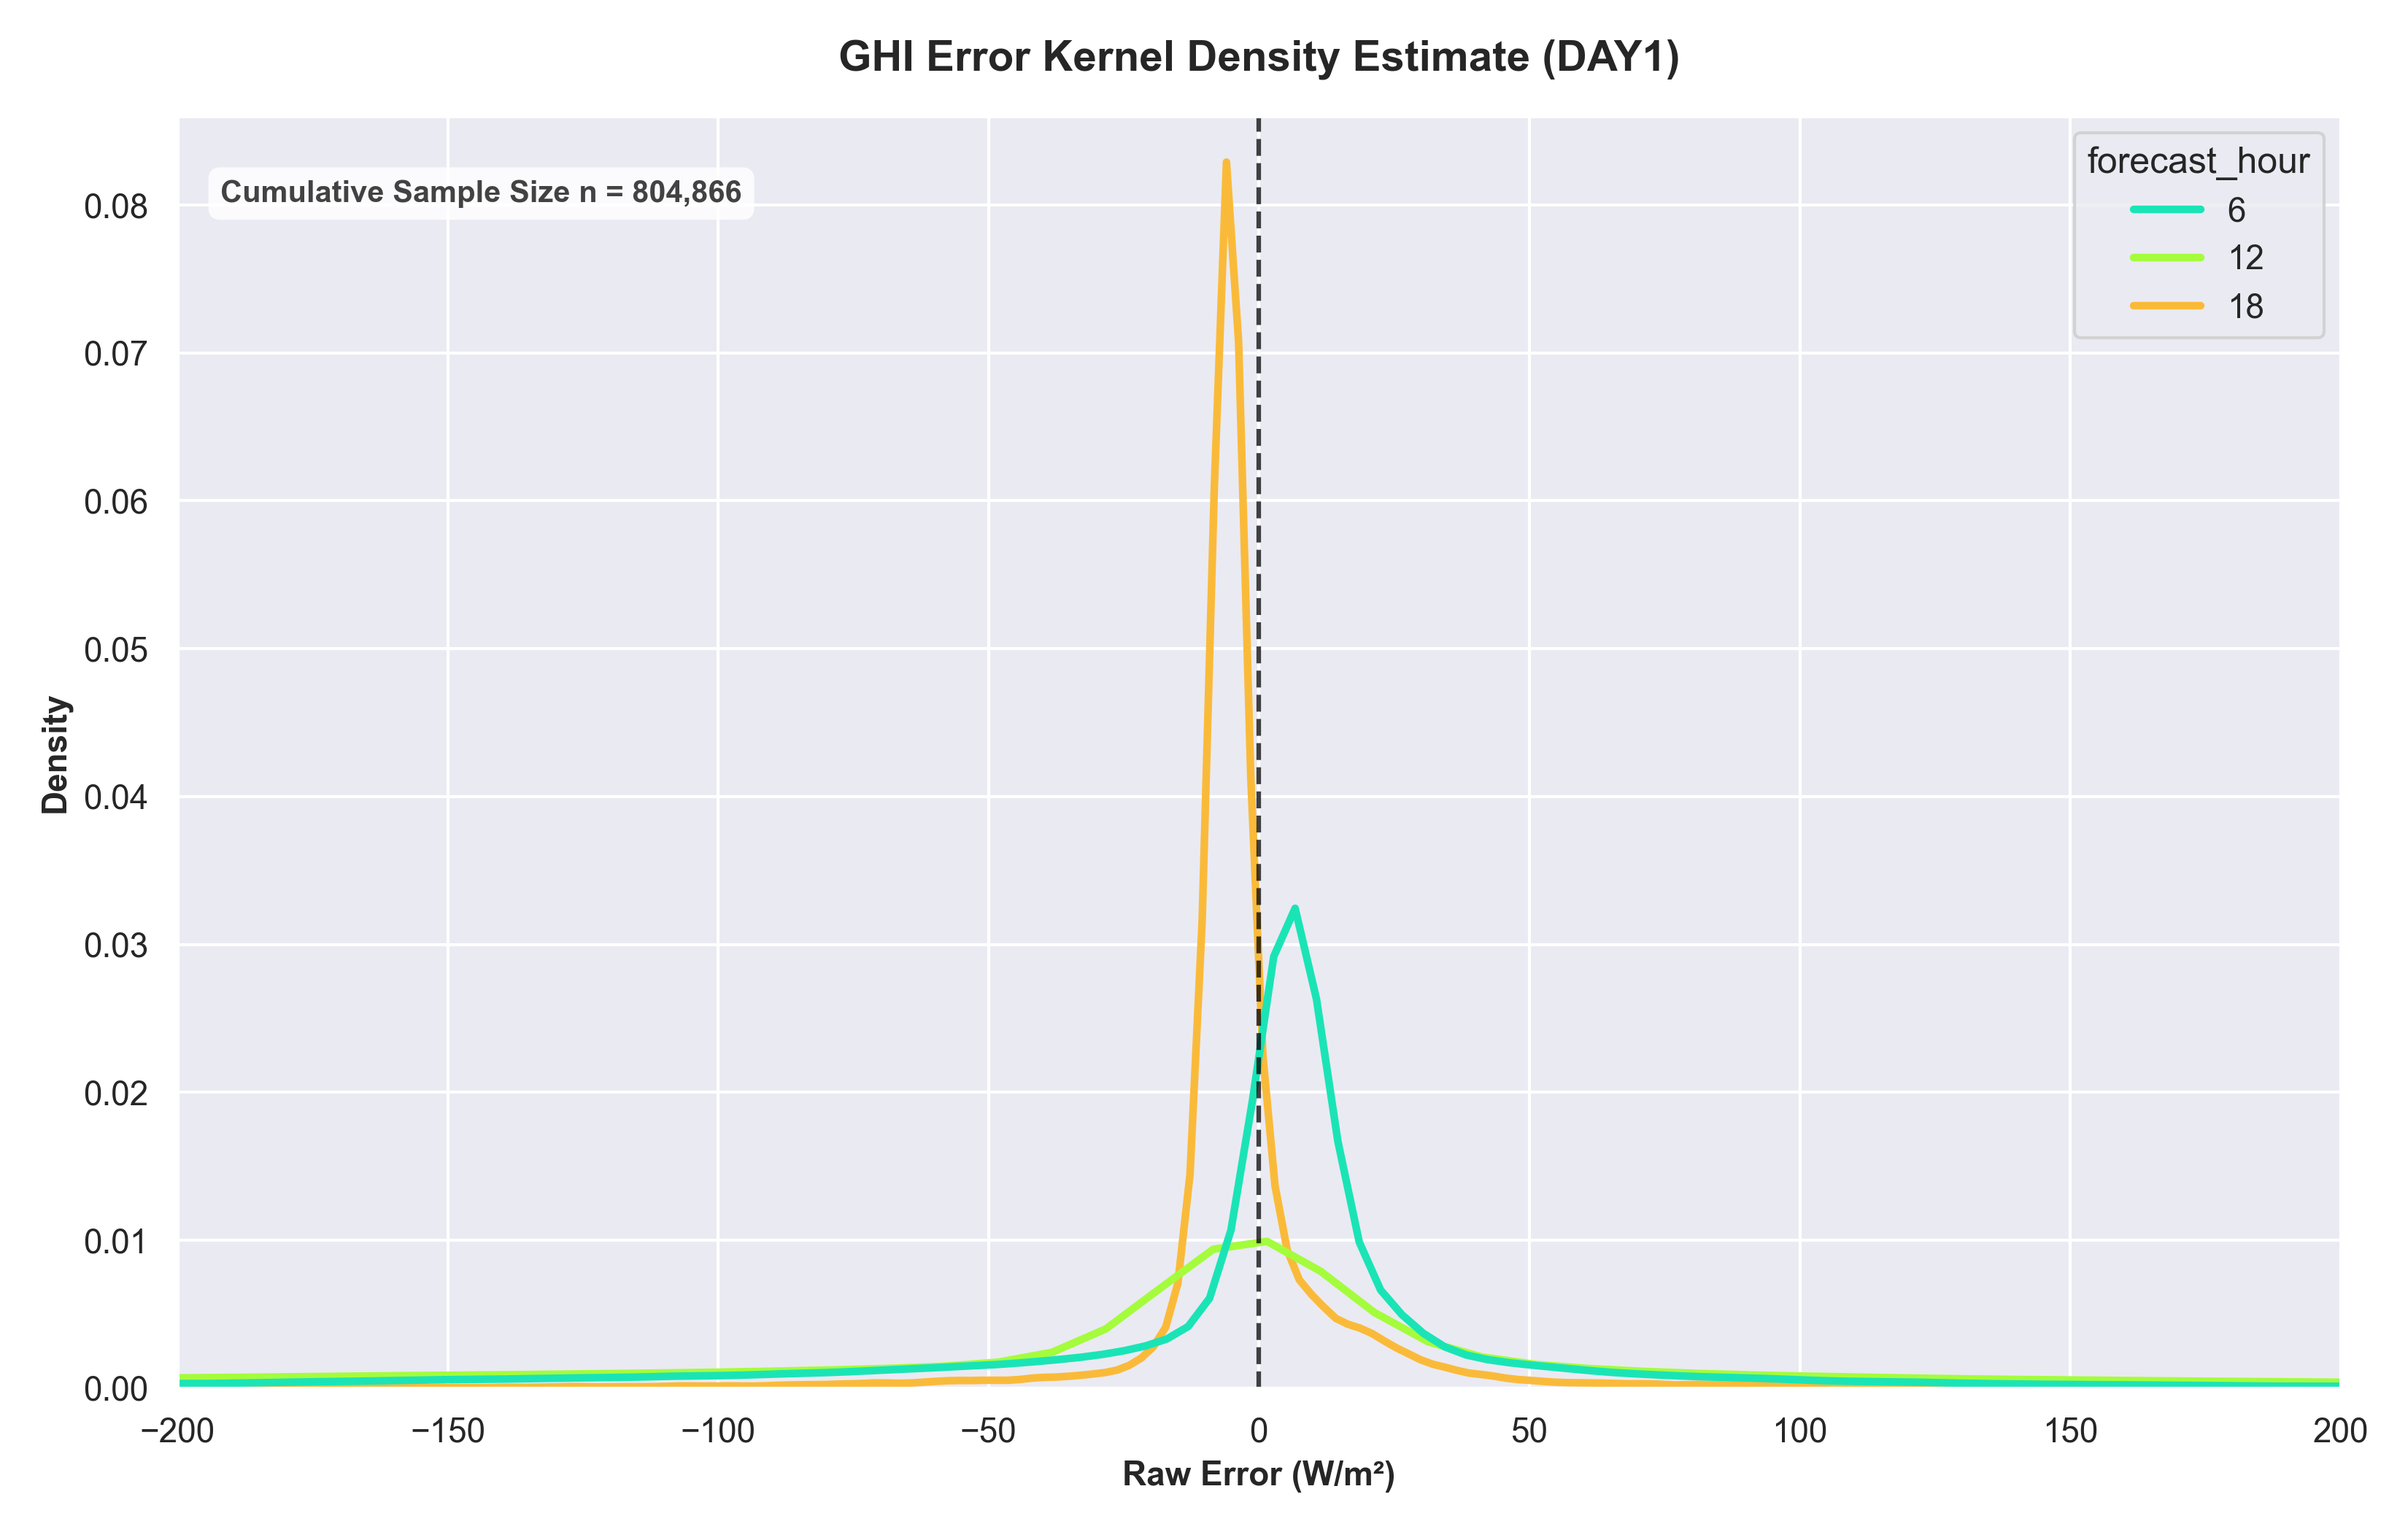
\includegraphics[width=0.49\textwidth]{figures/KDE_GRAPHS_RAW/ghi_kde_day1.png}\hfill
  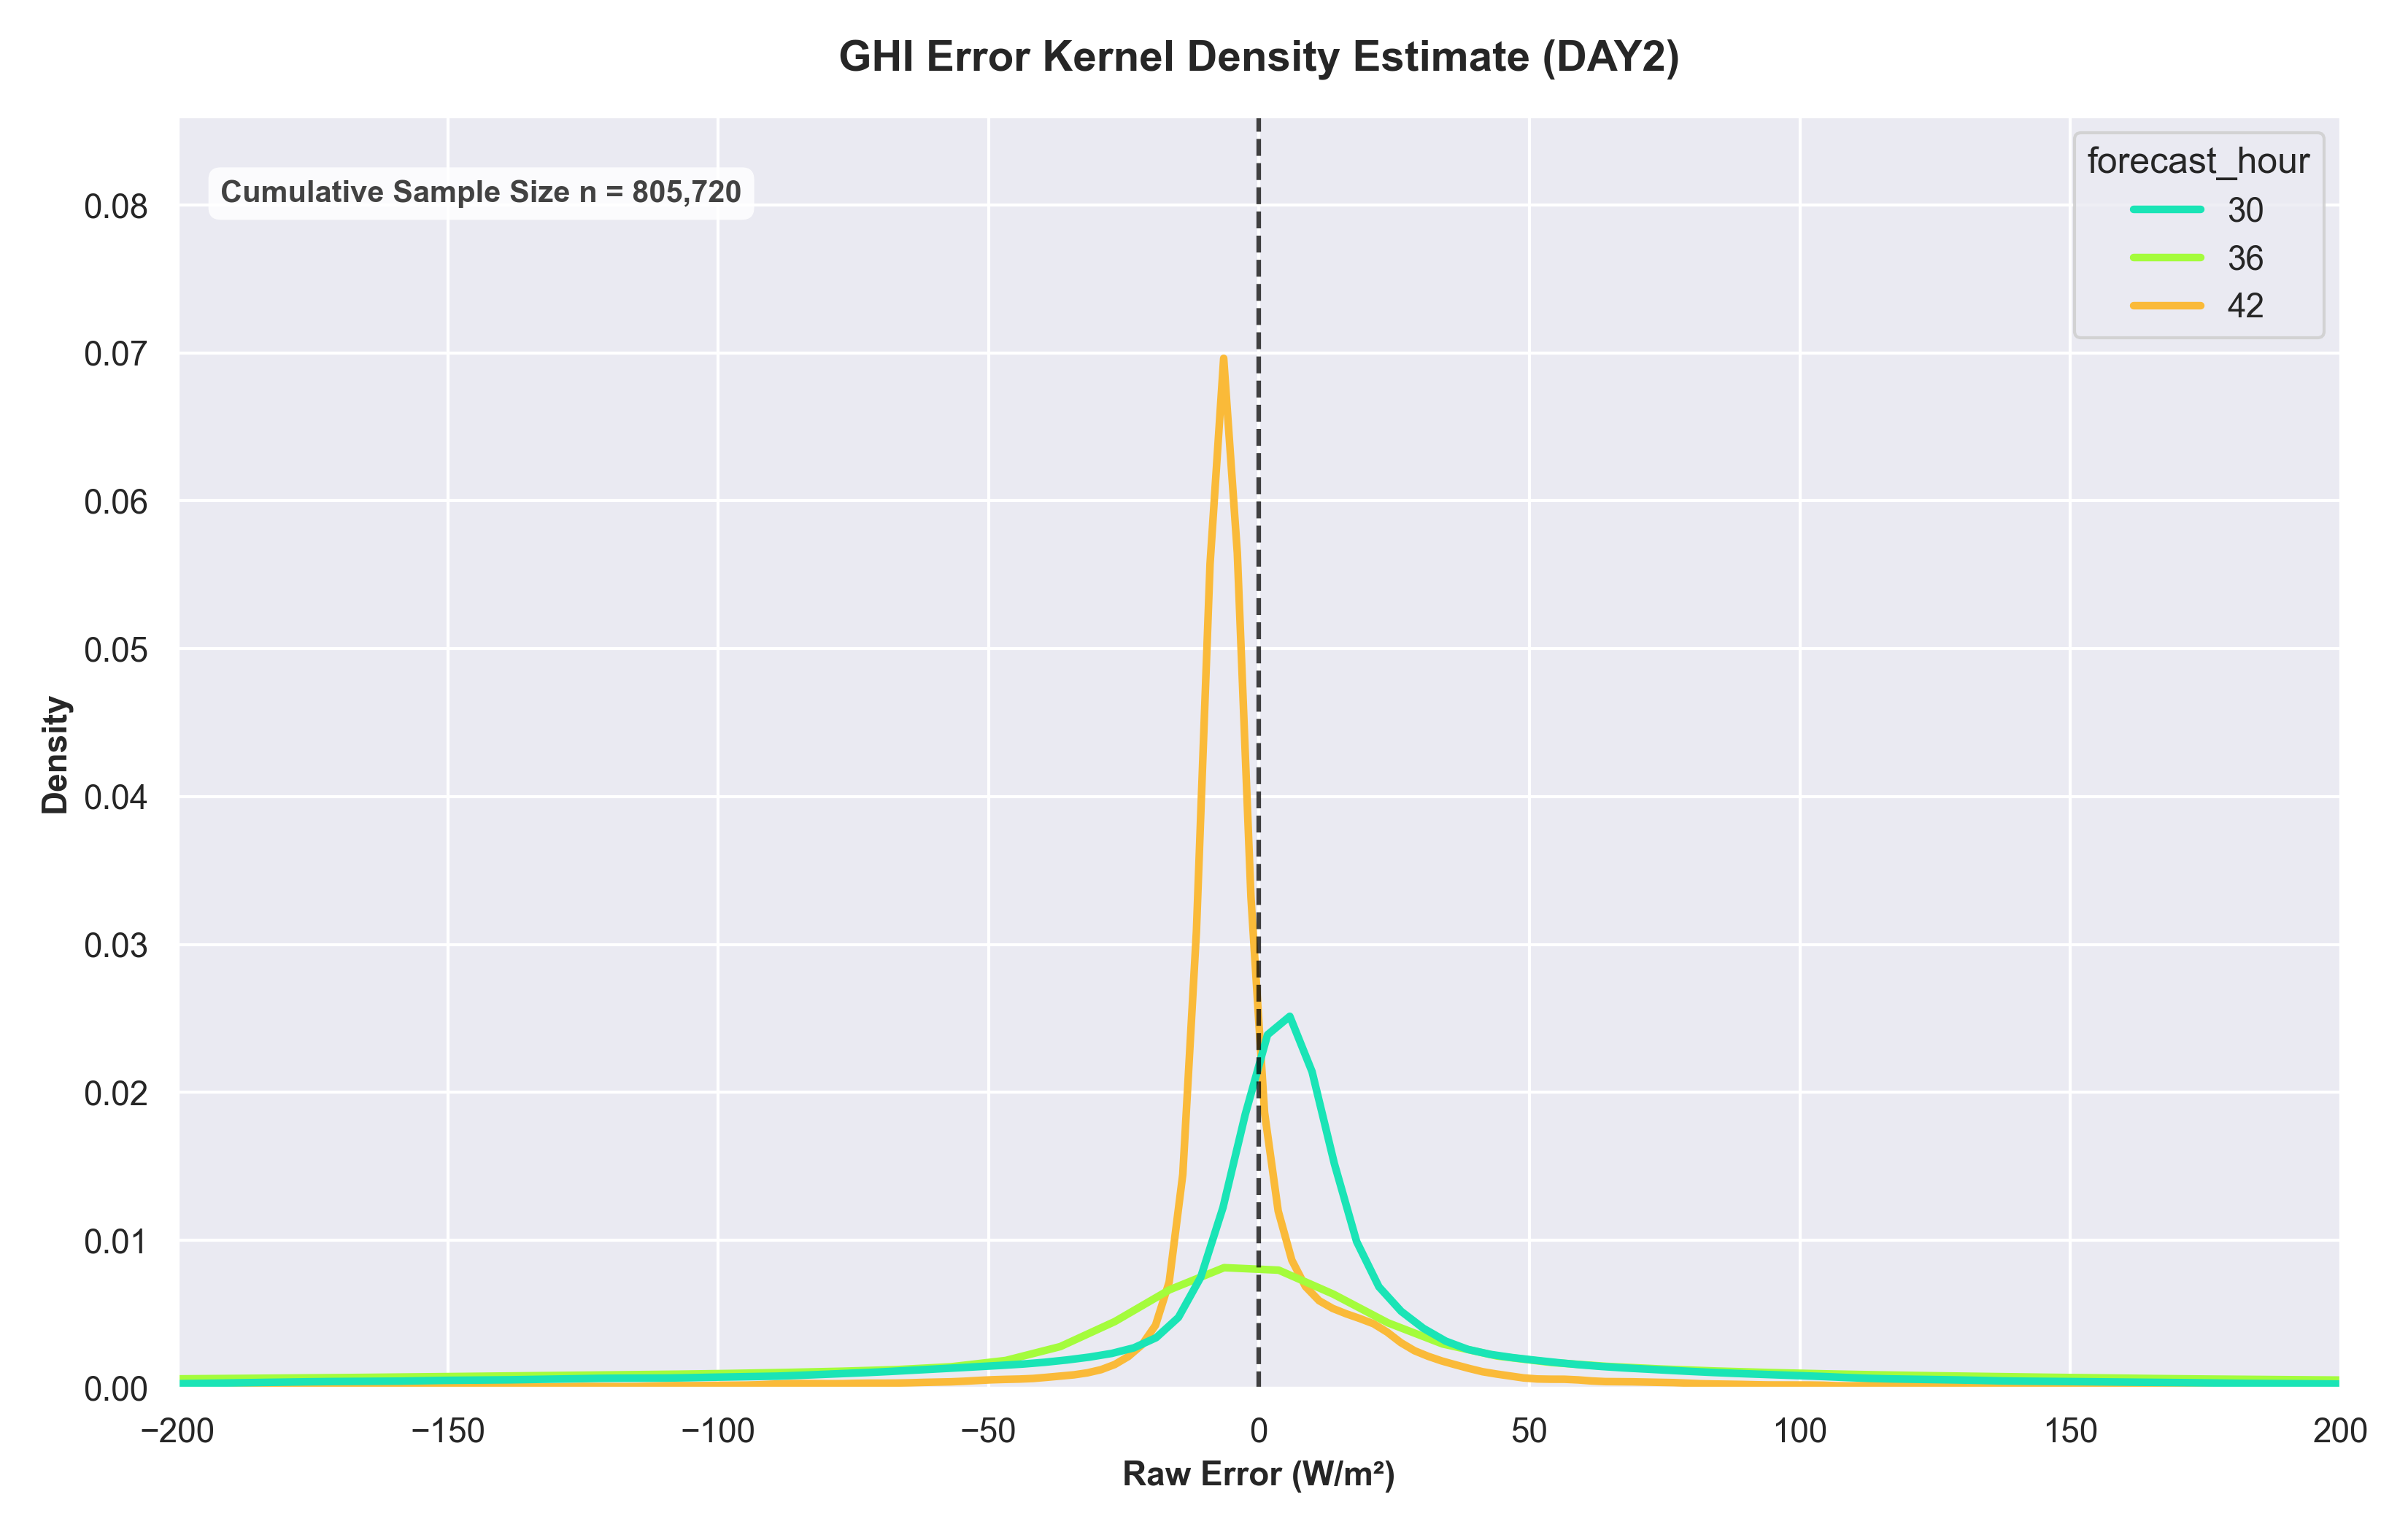
\includegraphics[width=0.49\textwidth]{figures/KDE_GRAPHS_RAW/ghi_kde_day2.png}
  \caption{Kernel Density Estimation (KDE) of Global Horizontal Irradiance (GHI) forecast errors for Day 1 (left) and Day 2 (right).}
  \label{fig:kde_ghi}
\end{figure}

\begin{figure}[H]
  \centering
  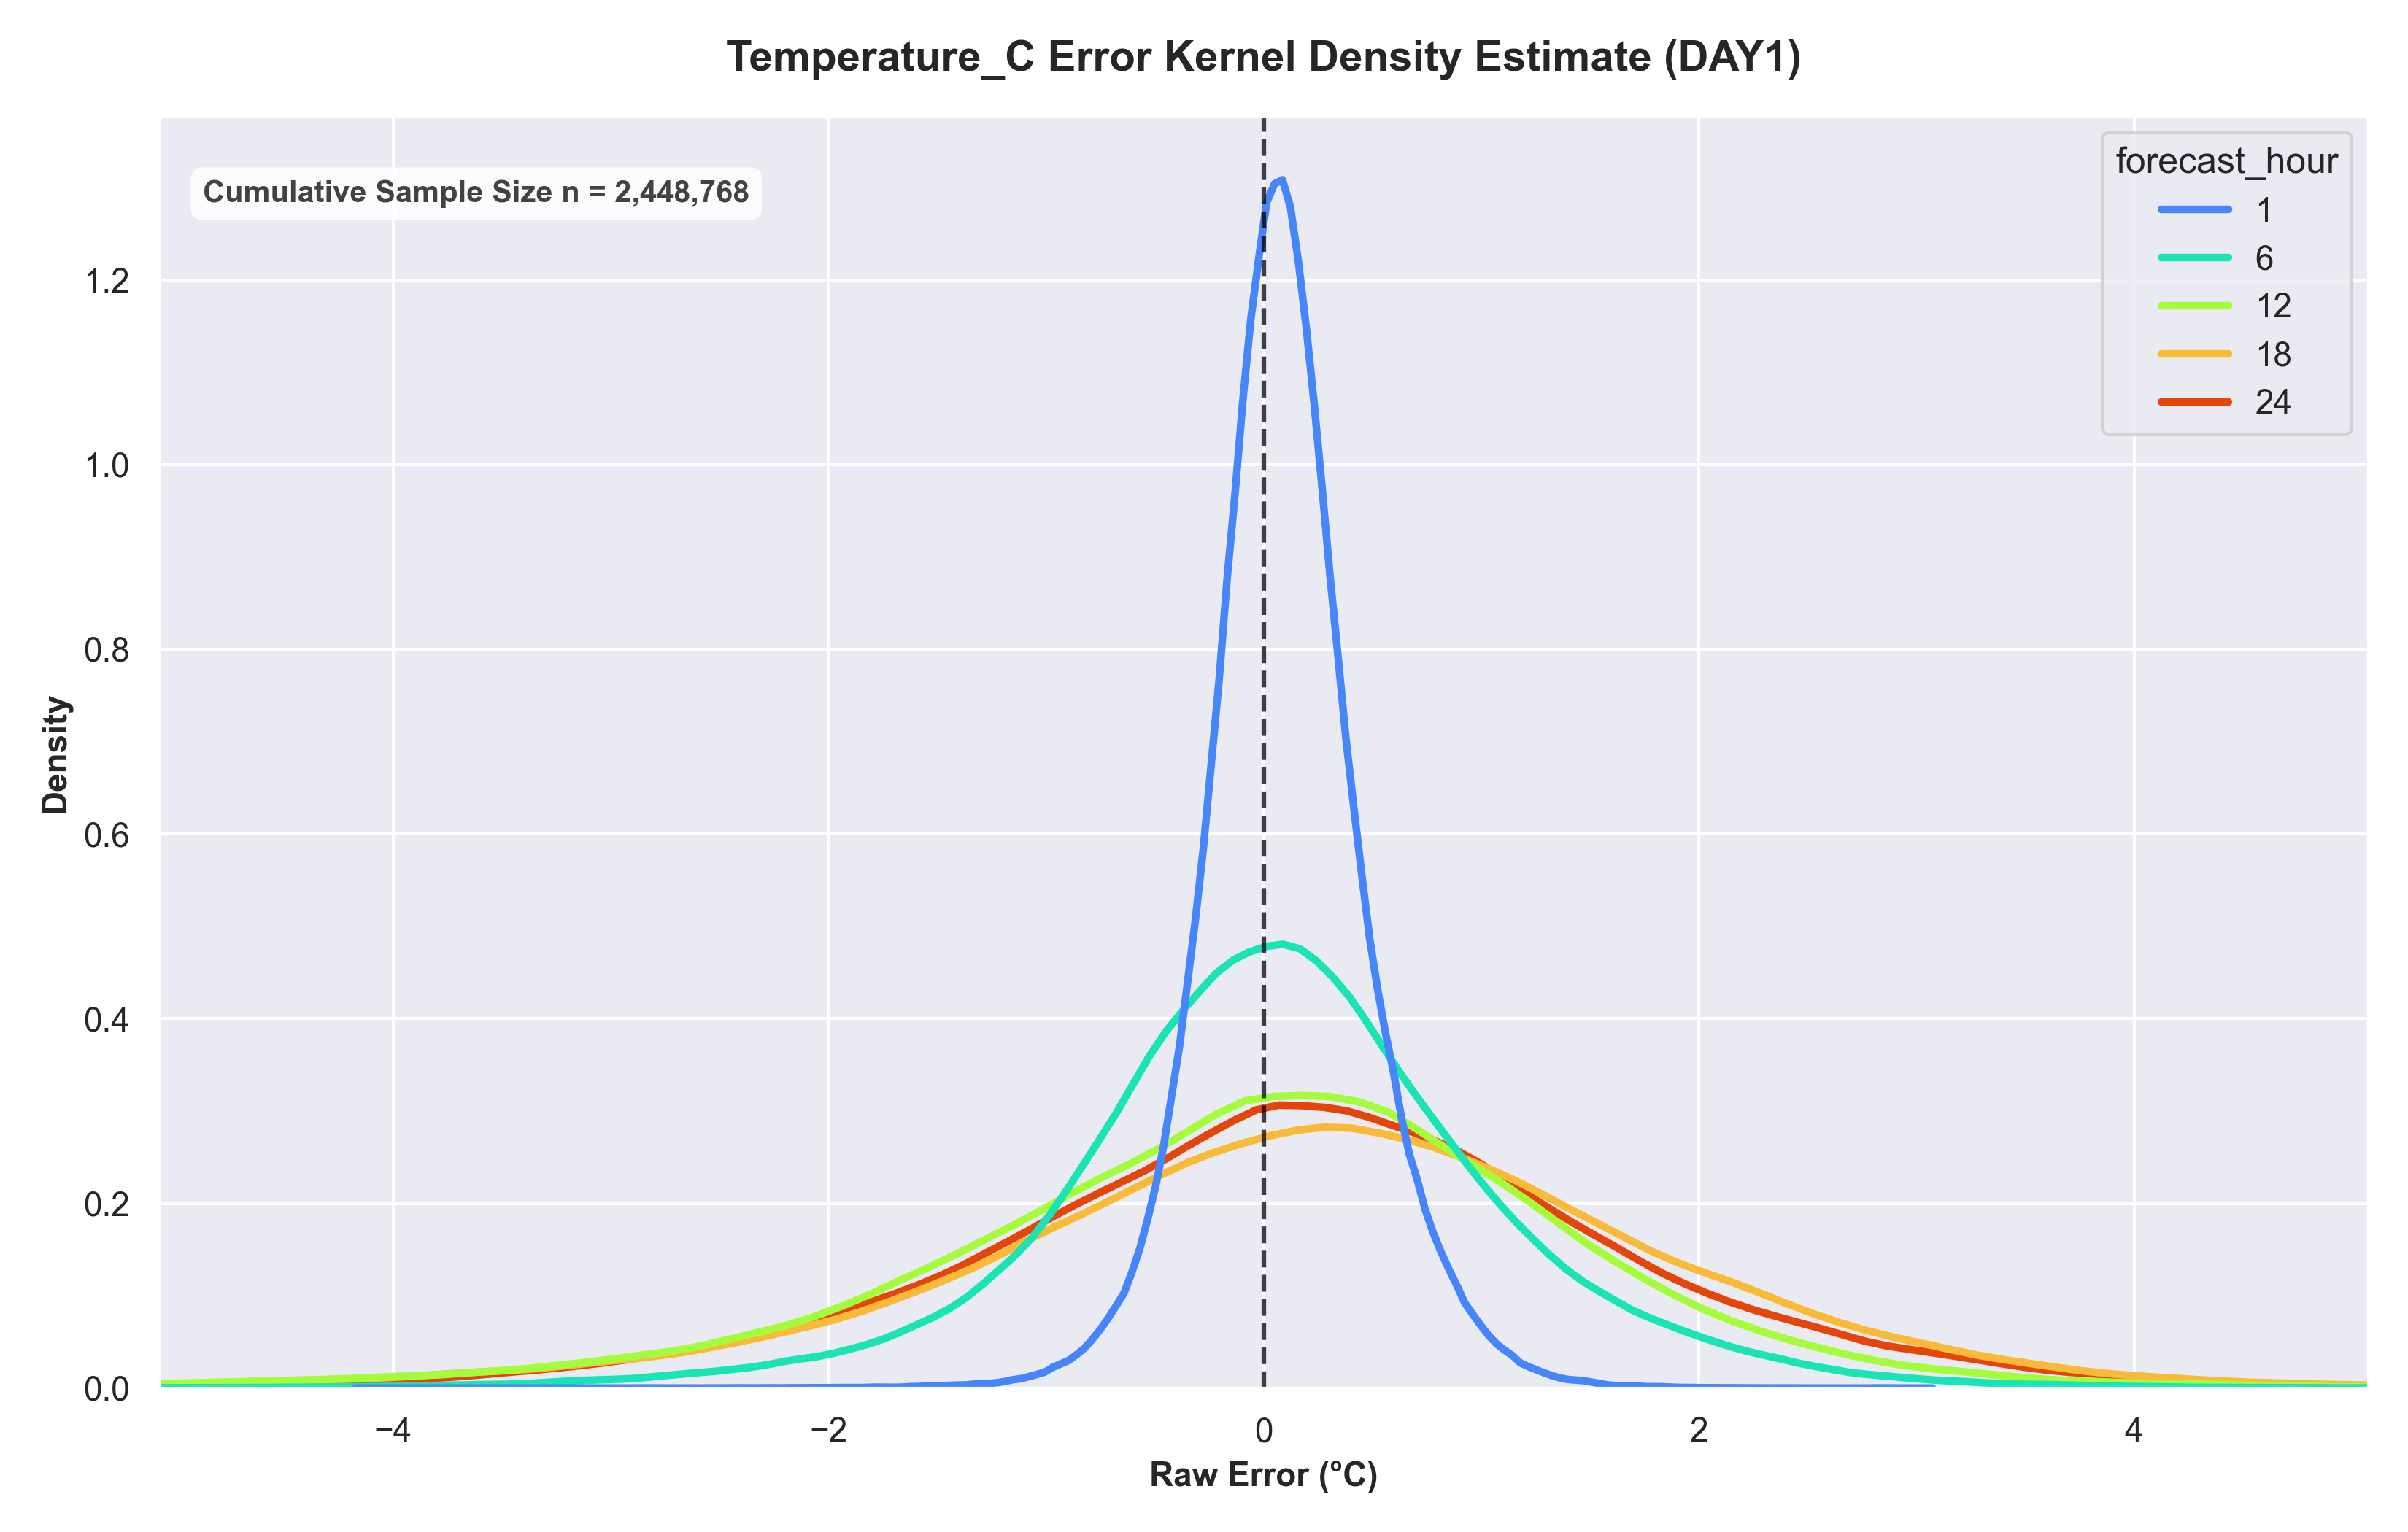
\includegraphics[width=0.49\textwidth]{figures/KDE_GRAPHS_RAW/temperature_c_kde_day1.png}\hfill
  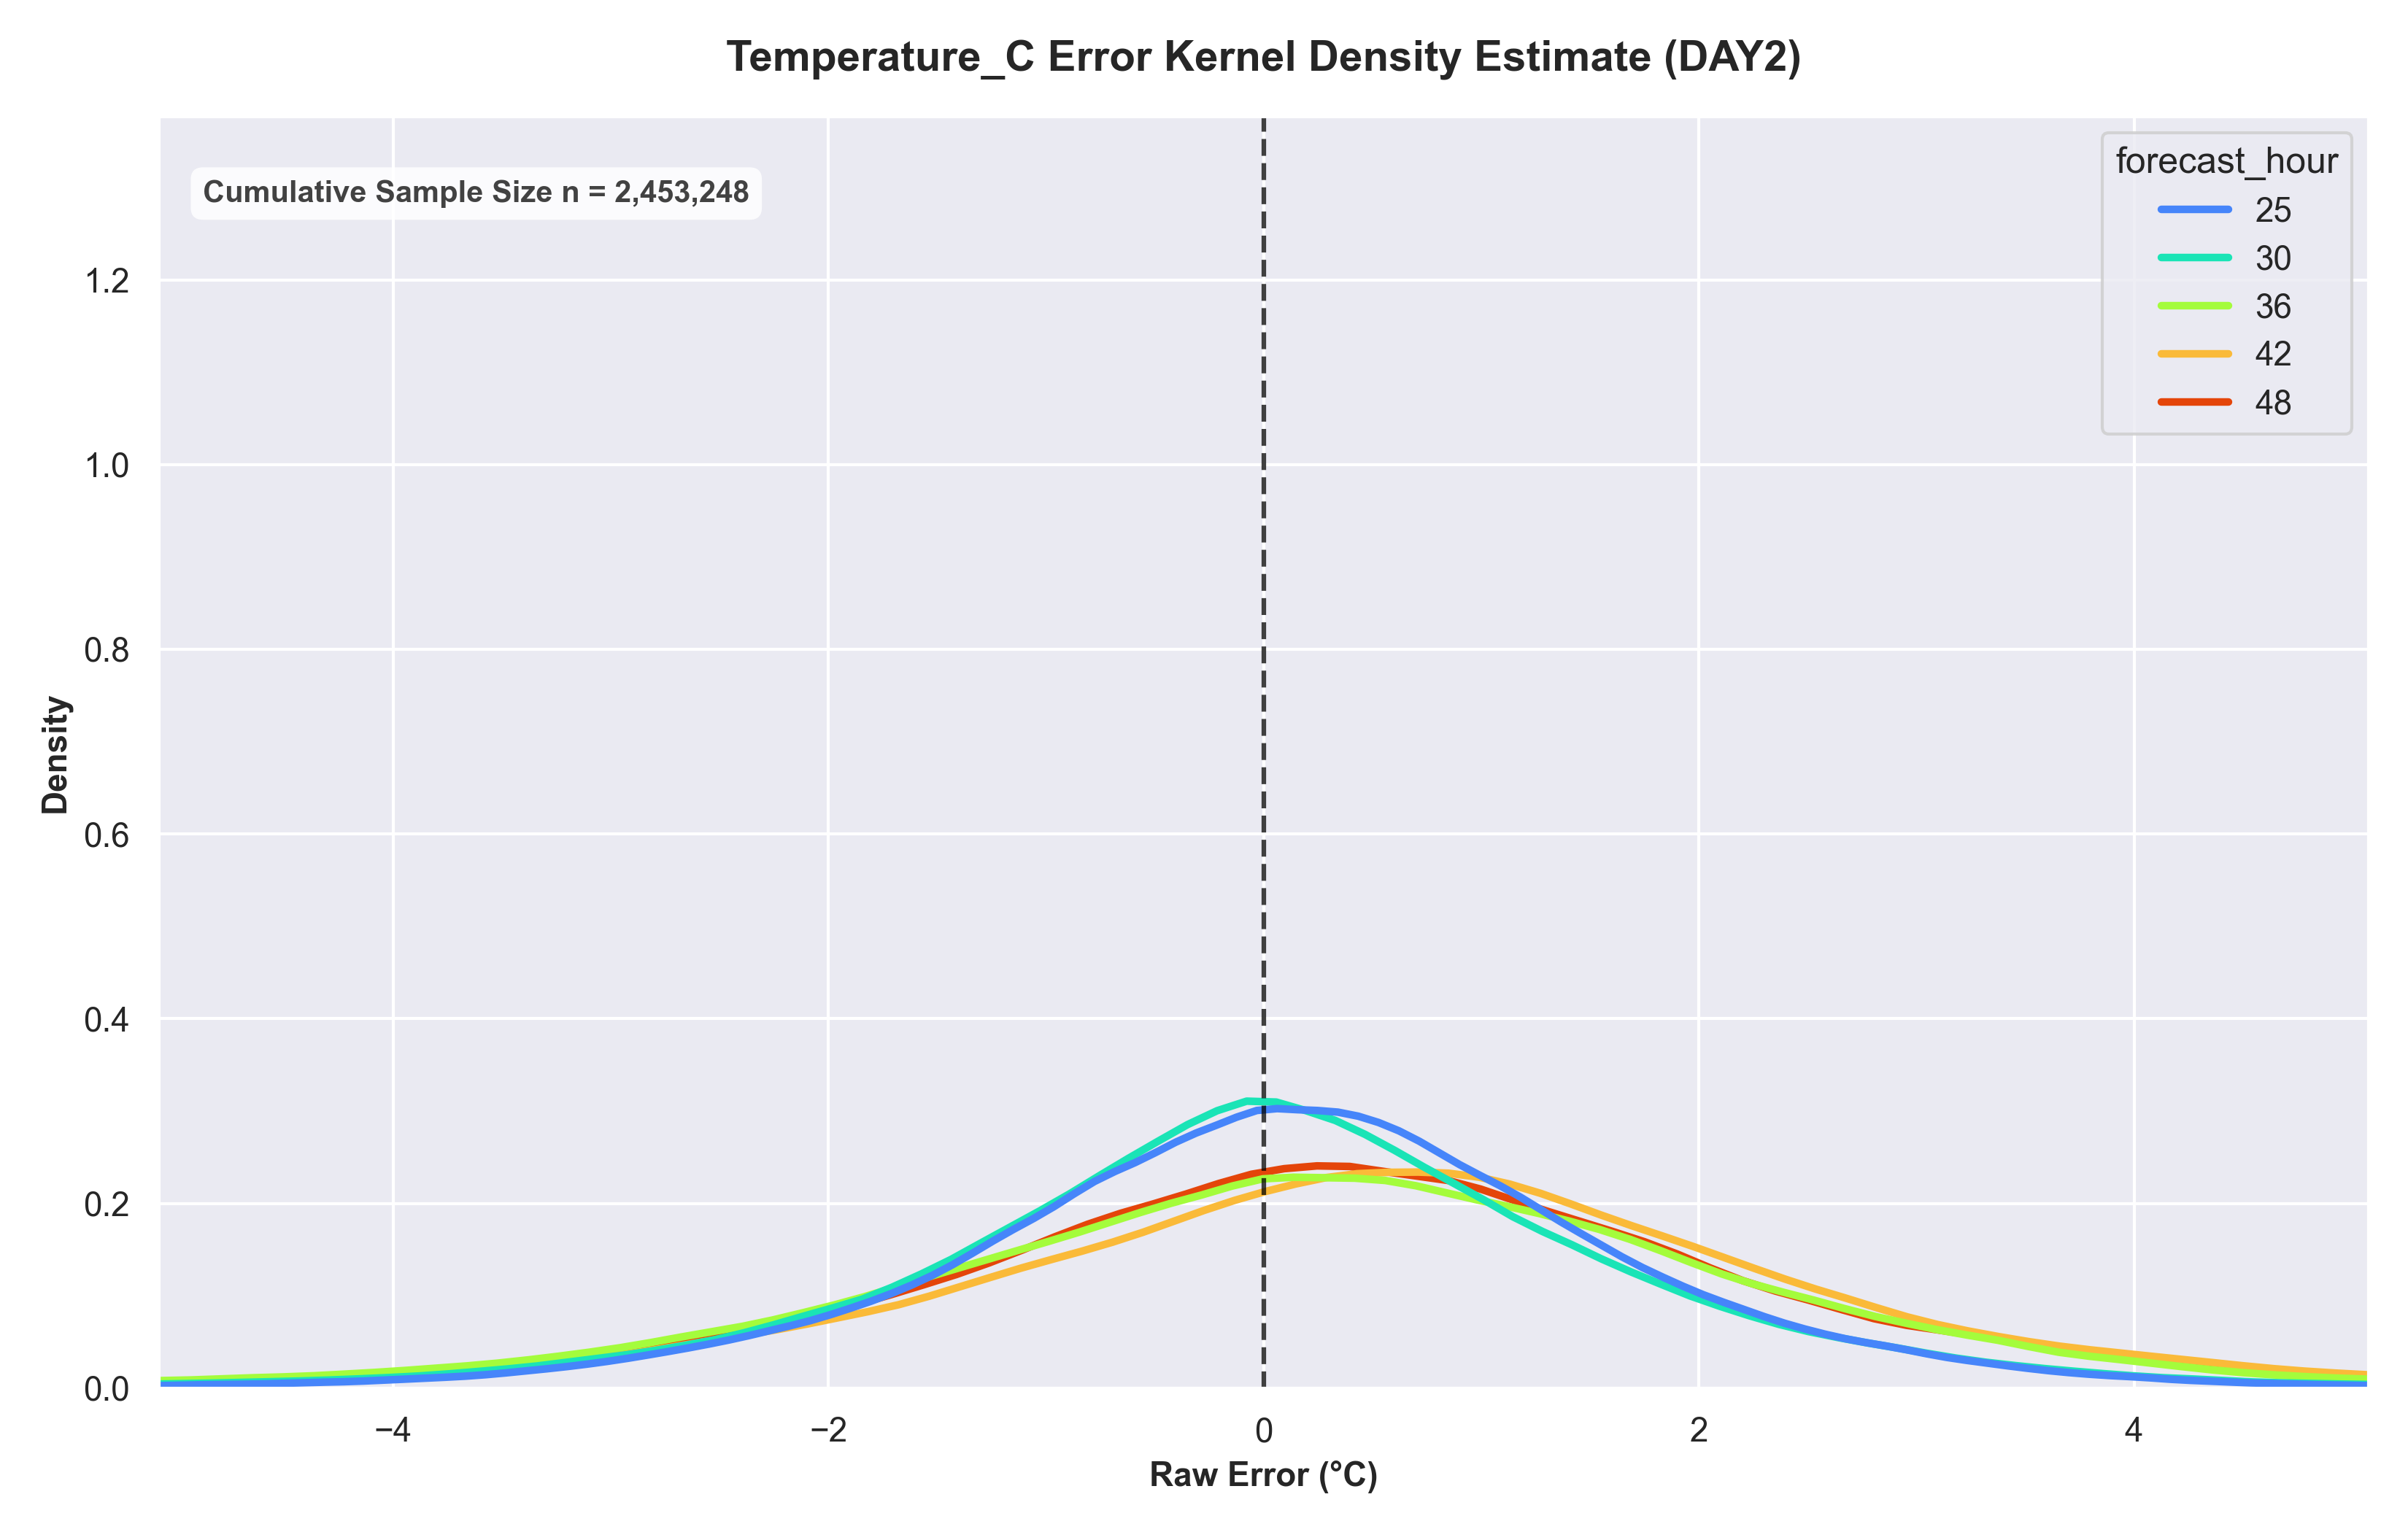
\includegraphics[width=0.49\textwidth]{figures/KDE_GRAPHS_RAW/temperature_c_kde_day2.png}
  \caption{Kernel Density Estimation (KDE) of Temperature forecast errors for Day 1 (left) and Day 2 (right).}
  \label{fig:kde_temp}
\end{figure}

\begin{figure}[H]
  \centering
  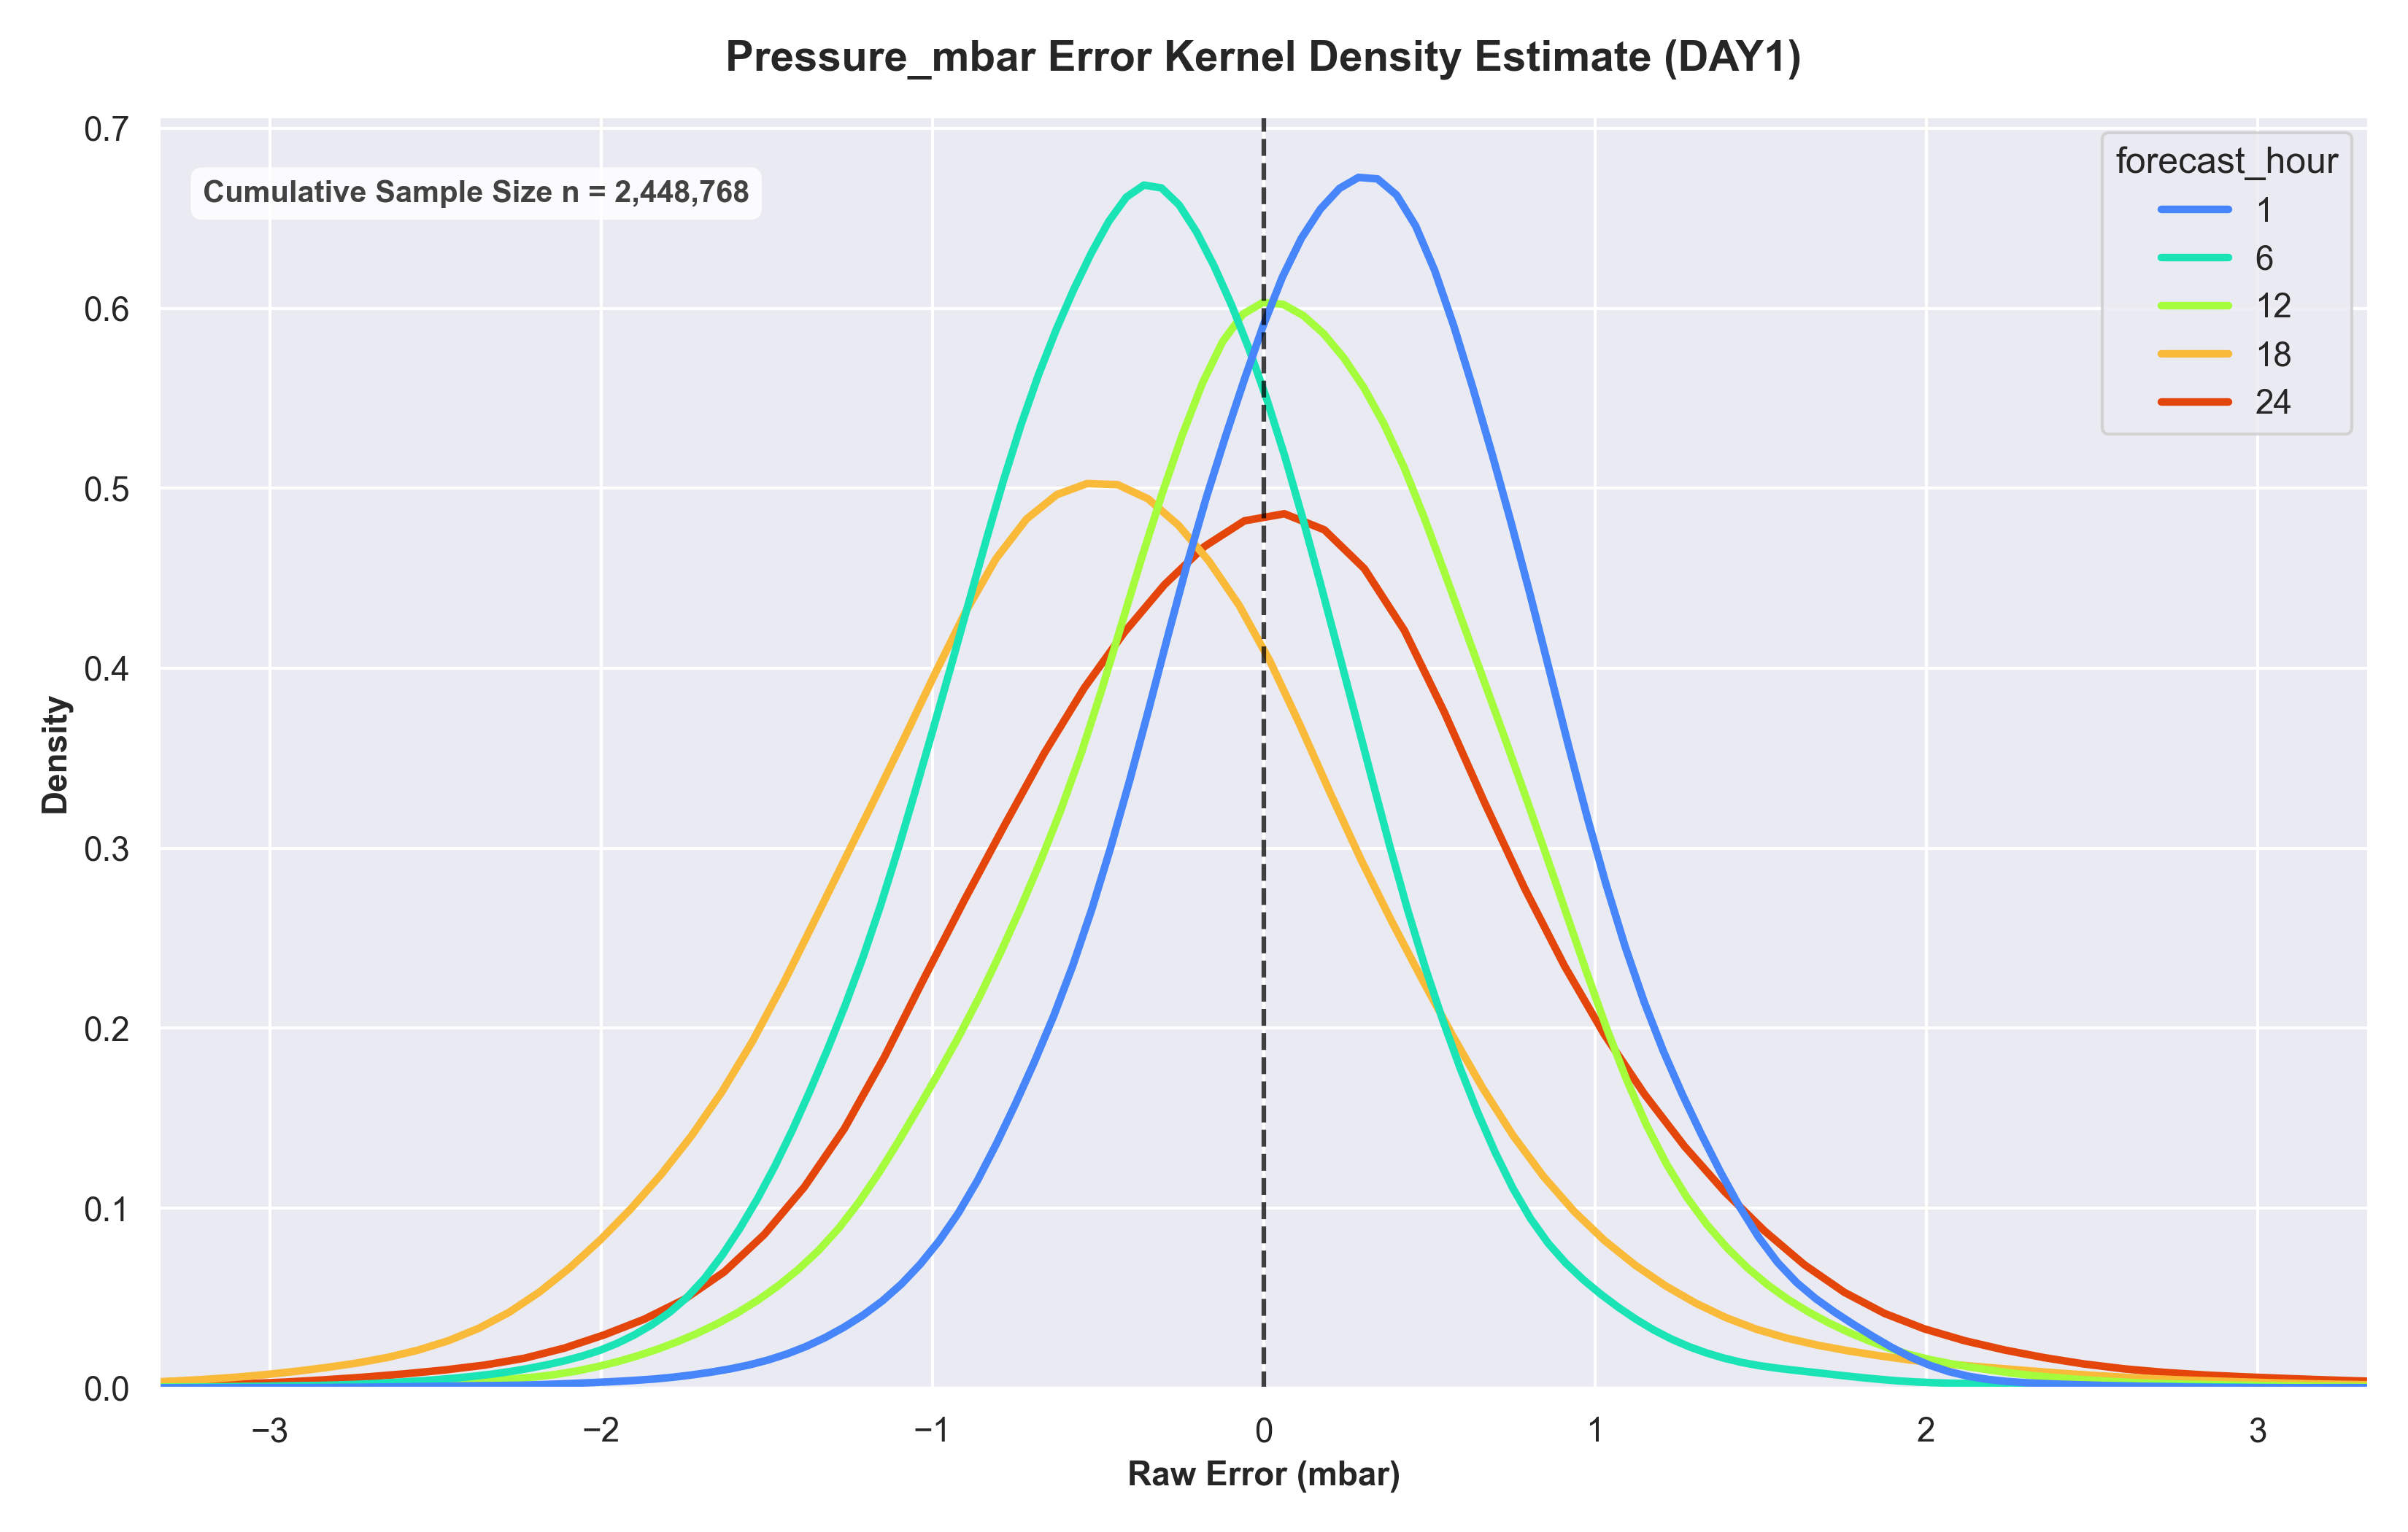
\includegraphics[width=0.49\textwidth]{figures/KDE_GRAPHS_RAW/pressure_mbar_kde_day1.png}\hfill
  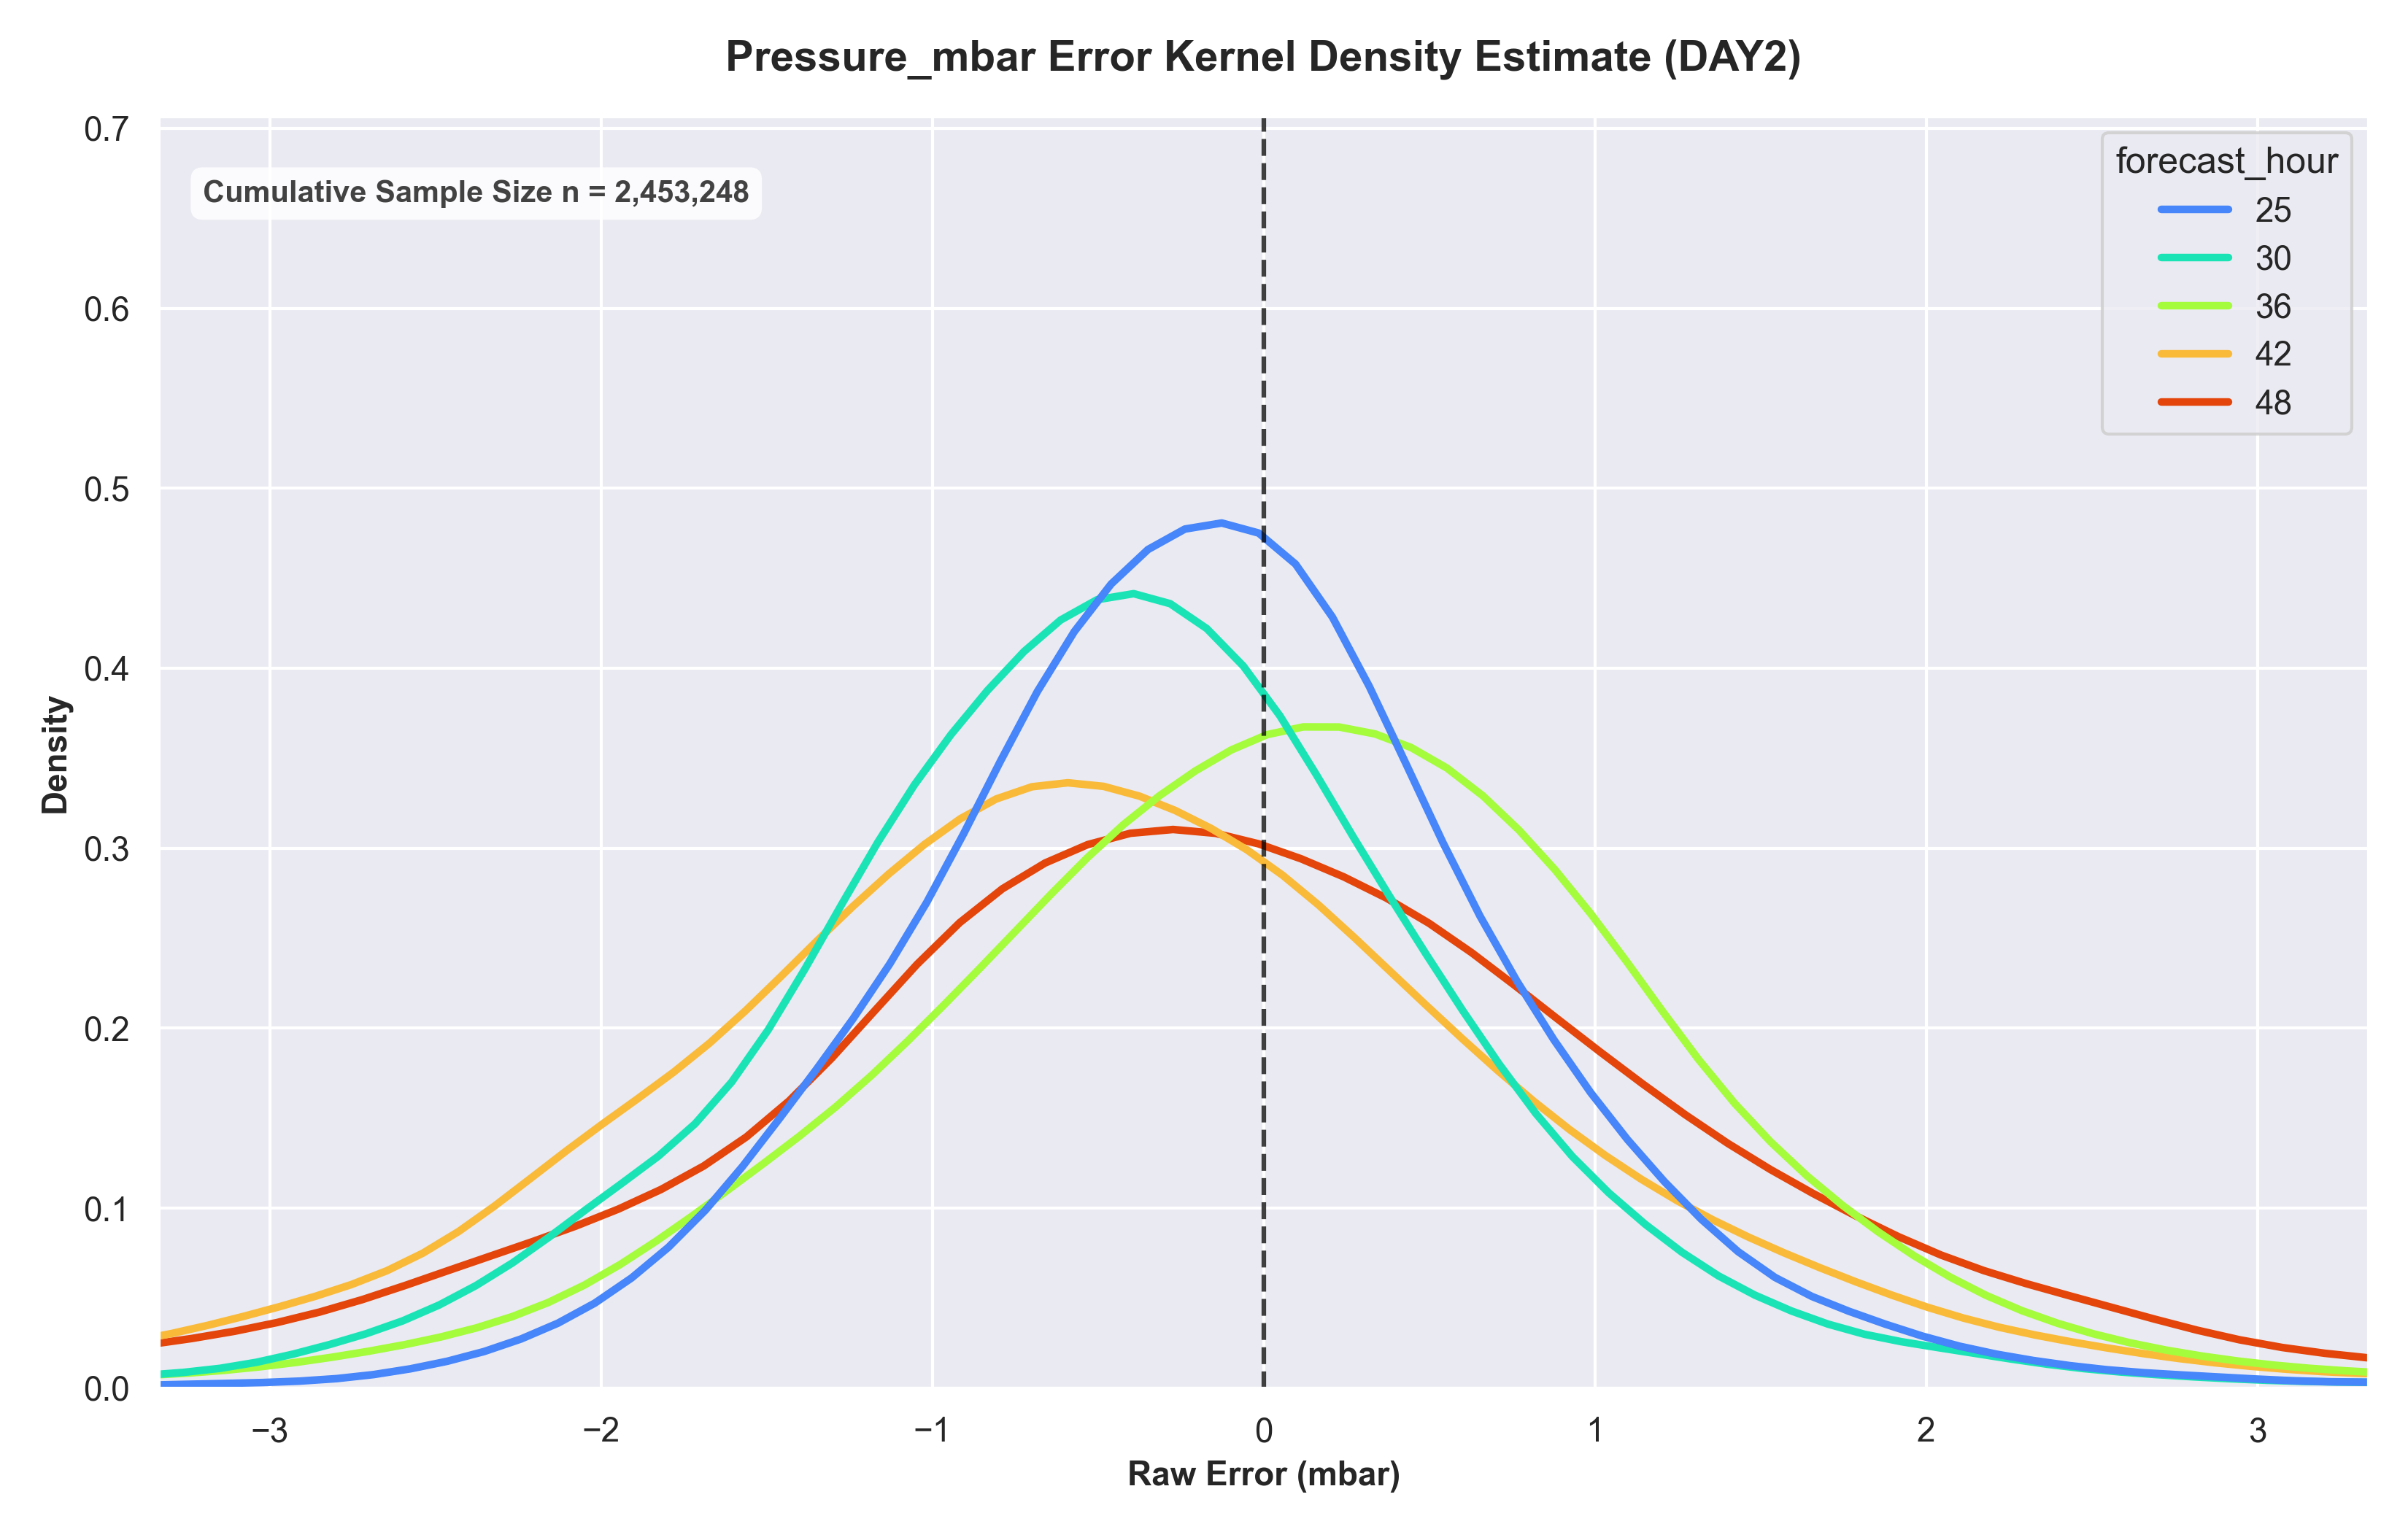
\includegraphics[width=0.49\textwidth]{figures/KDE_GRAPHS_RAW/pressure_mbar_kde_day2.png}
  \caption{Kernel Density Estimation (KDE) of Air Pressure forecast errors for Day 1 (left) and Day 2 (right).}
  \label{fig:kde_pressure}
\end{figure}

\begin{figure}[H]
  \centering
  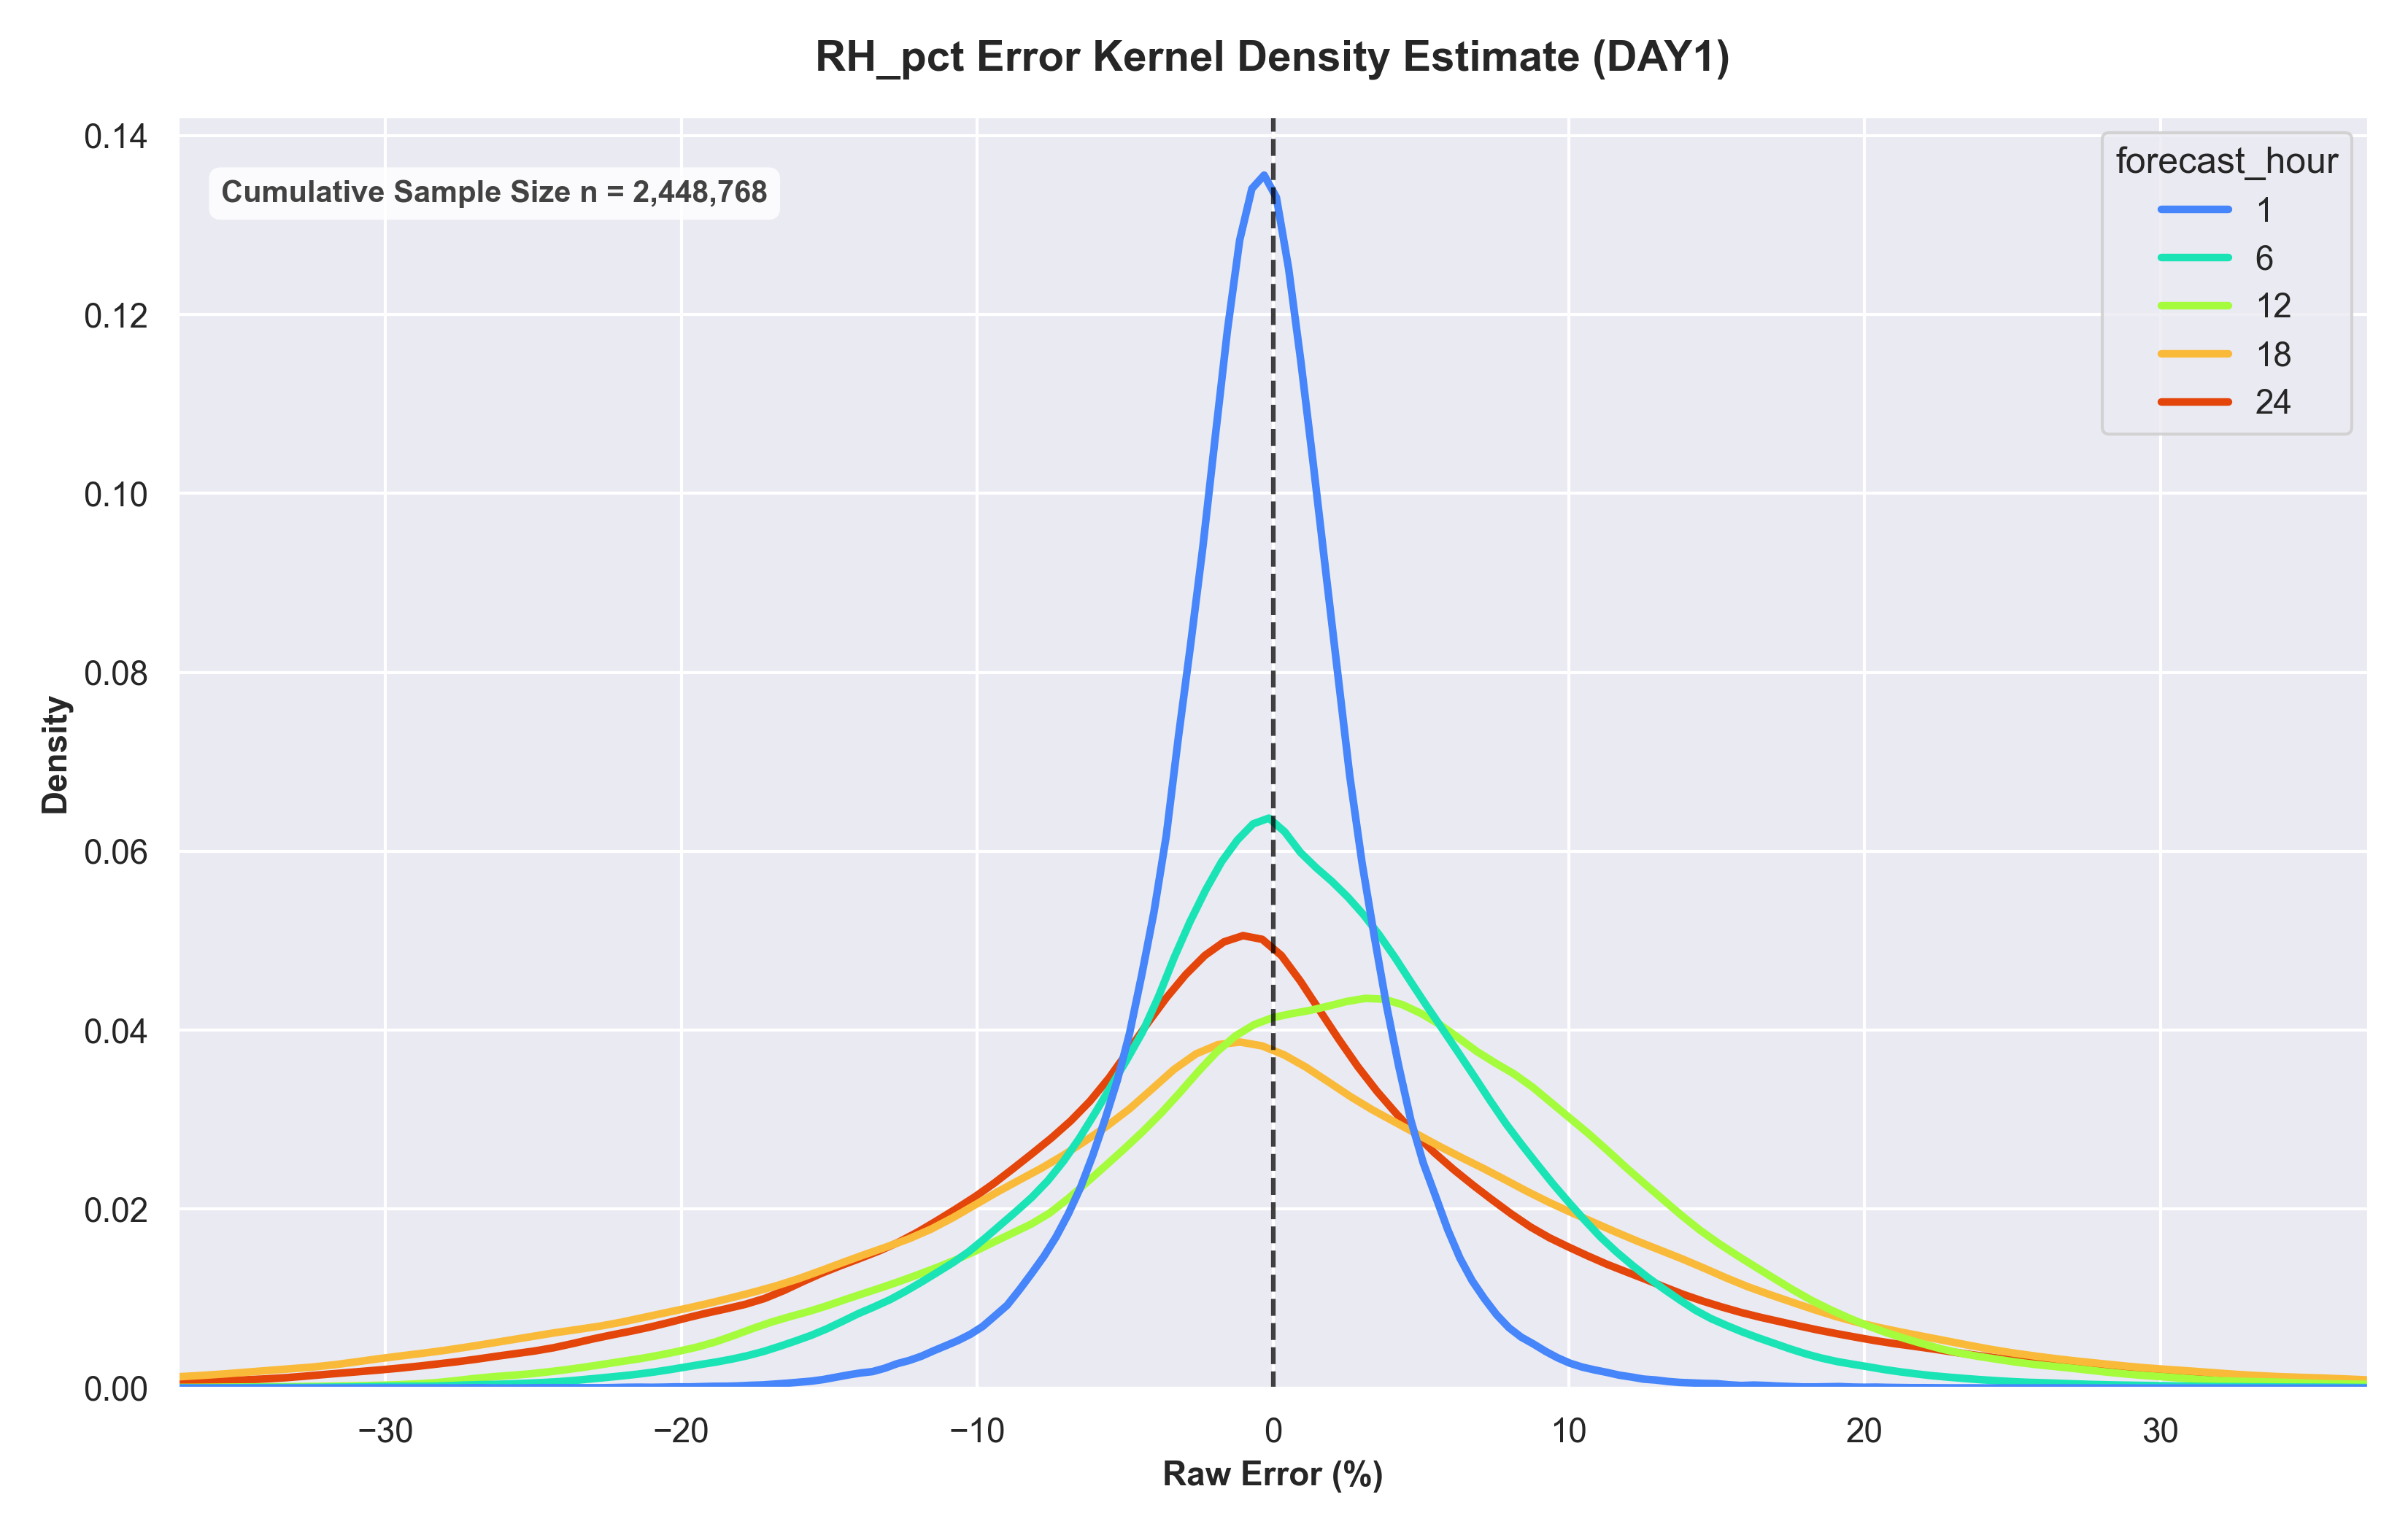
\includegraphics[width=0.49\textwidth]{figures/KDE_GRAPHS_RAW/rh_pct_kde_day1.png}\hfill
  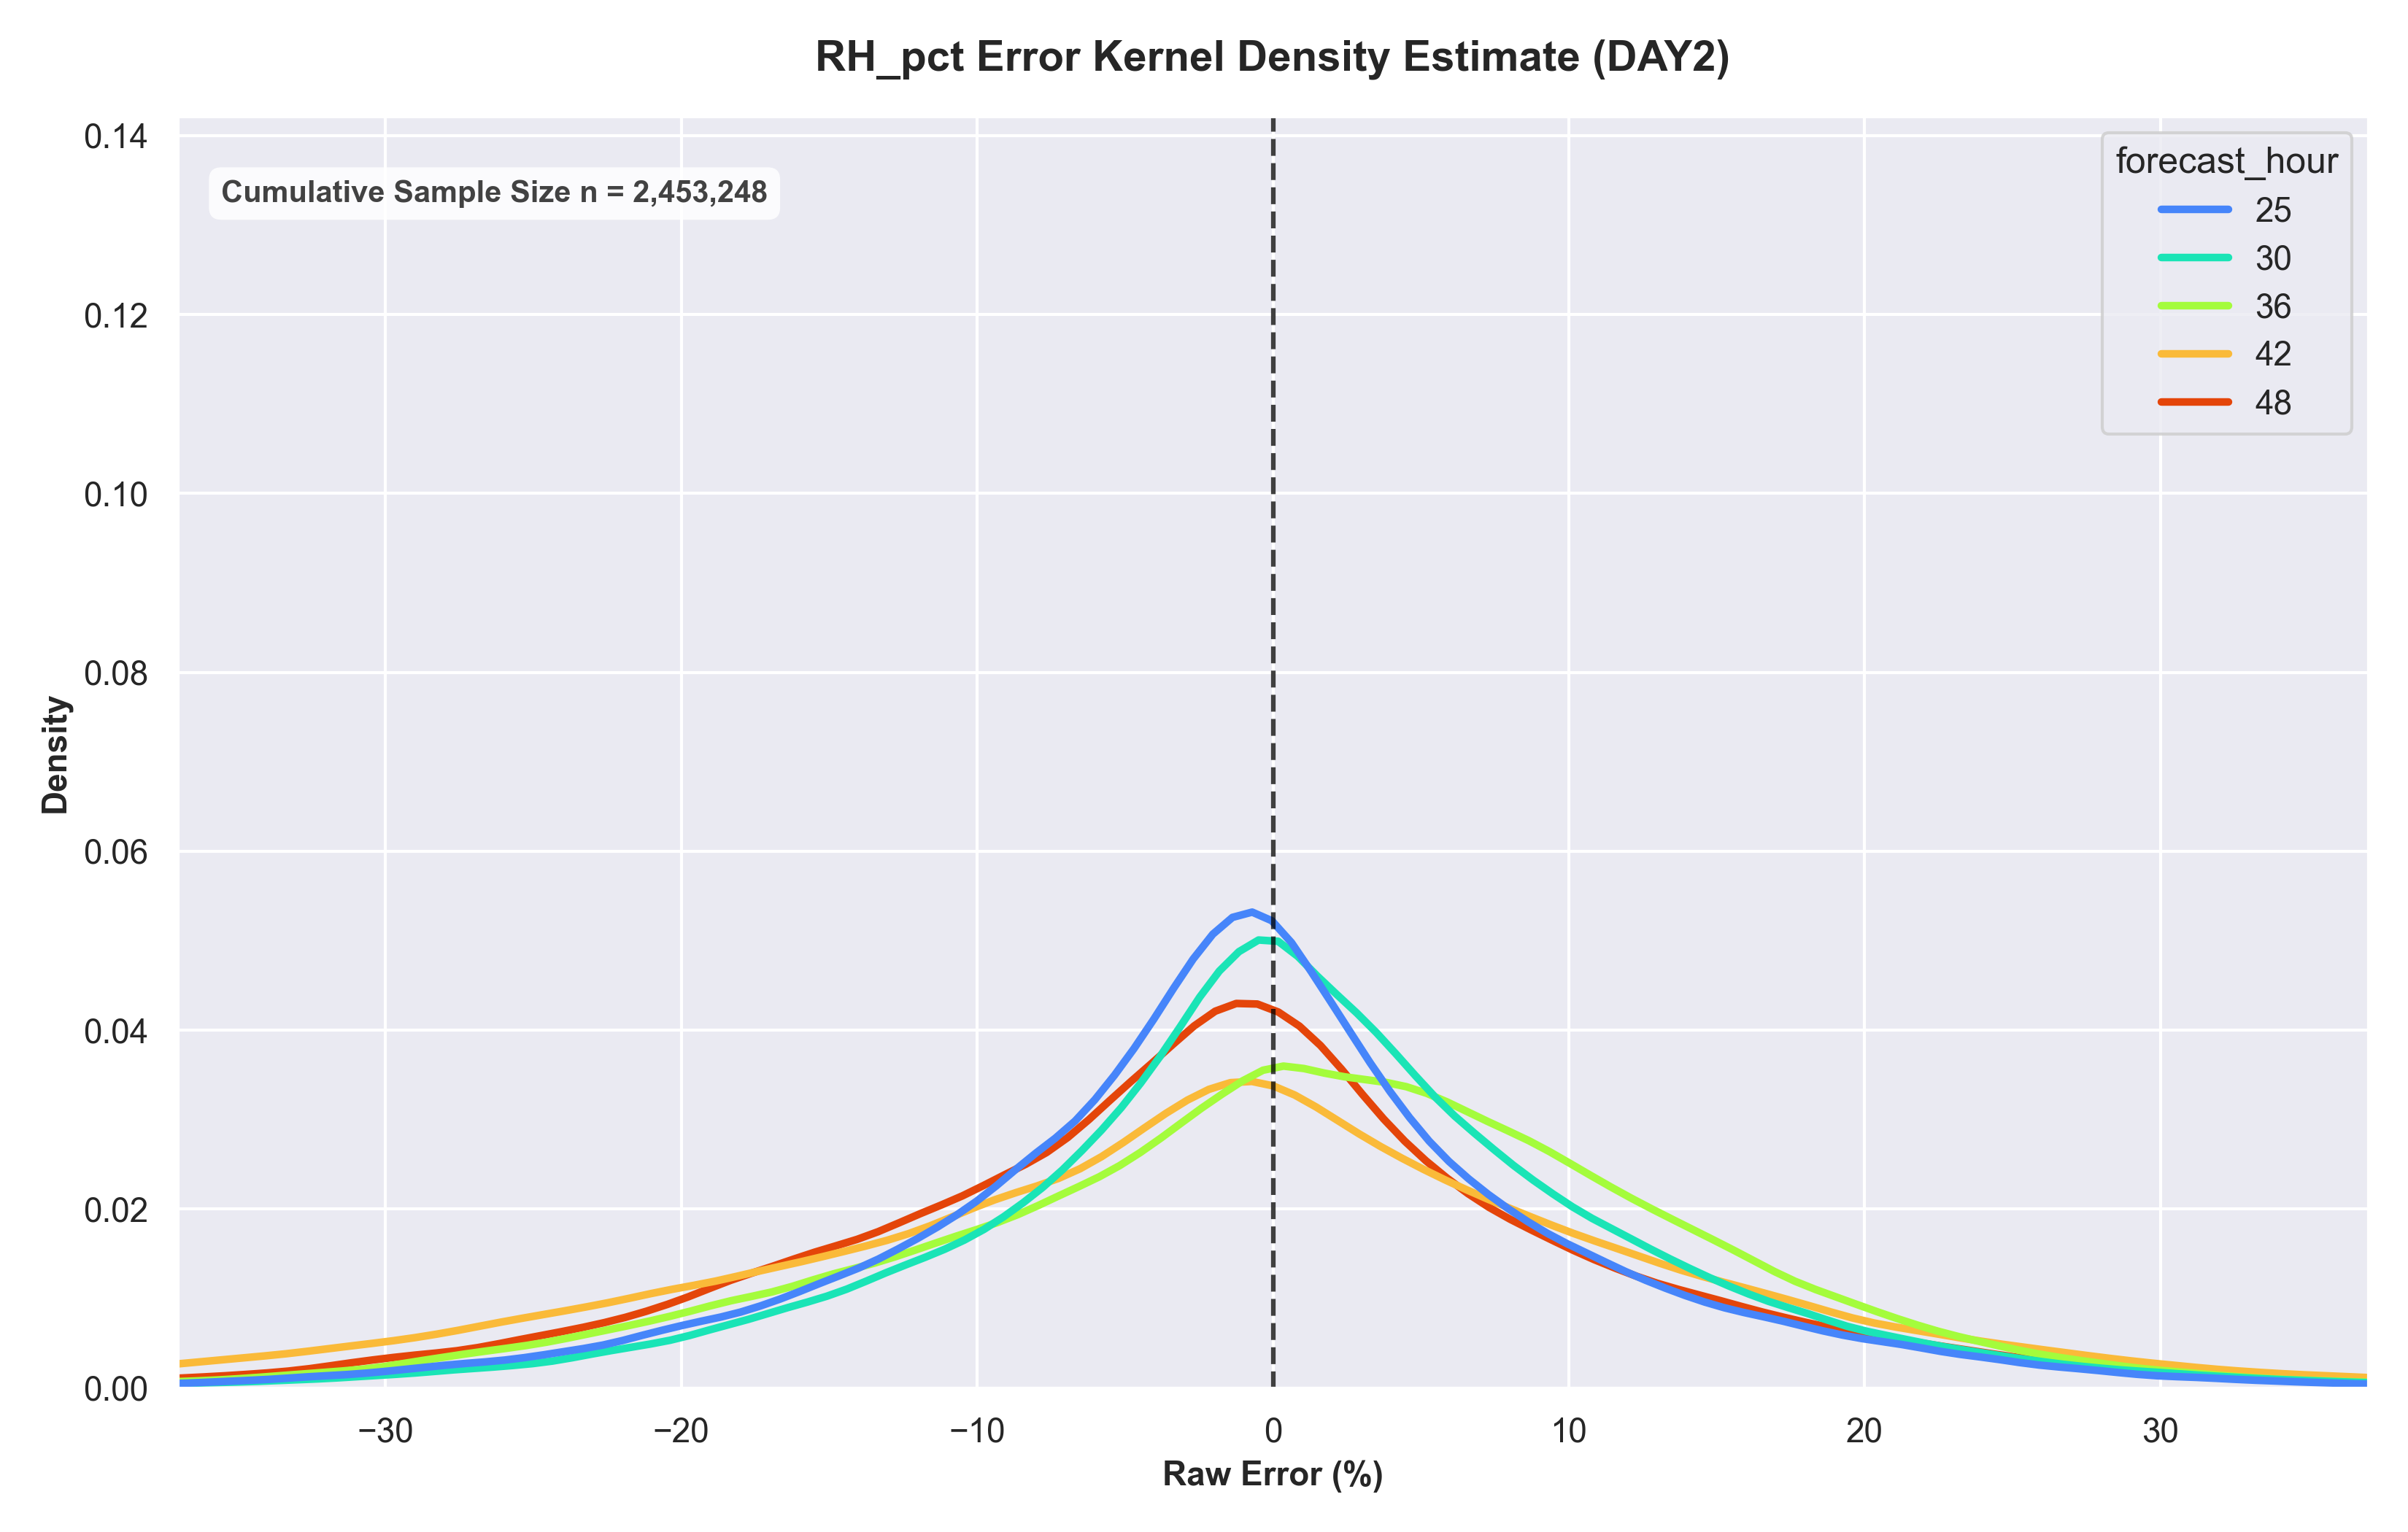
\includegraphics[width=0.49\textwidth]{figures/KDE_GRAPHS_RAW/rh_pct_kde_day2.png}
  \caption{Kernel Density Estimation (KDE) of Relative Humidity (RH) forecast errors for Day 1 (left) and Day 2 (right).}
  \label{fig:kde_rh}
\end{figure}

\begin{figure}[H]
  \centering
  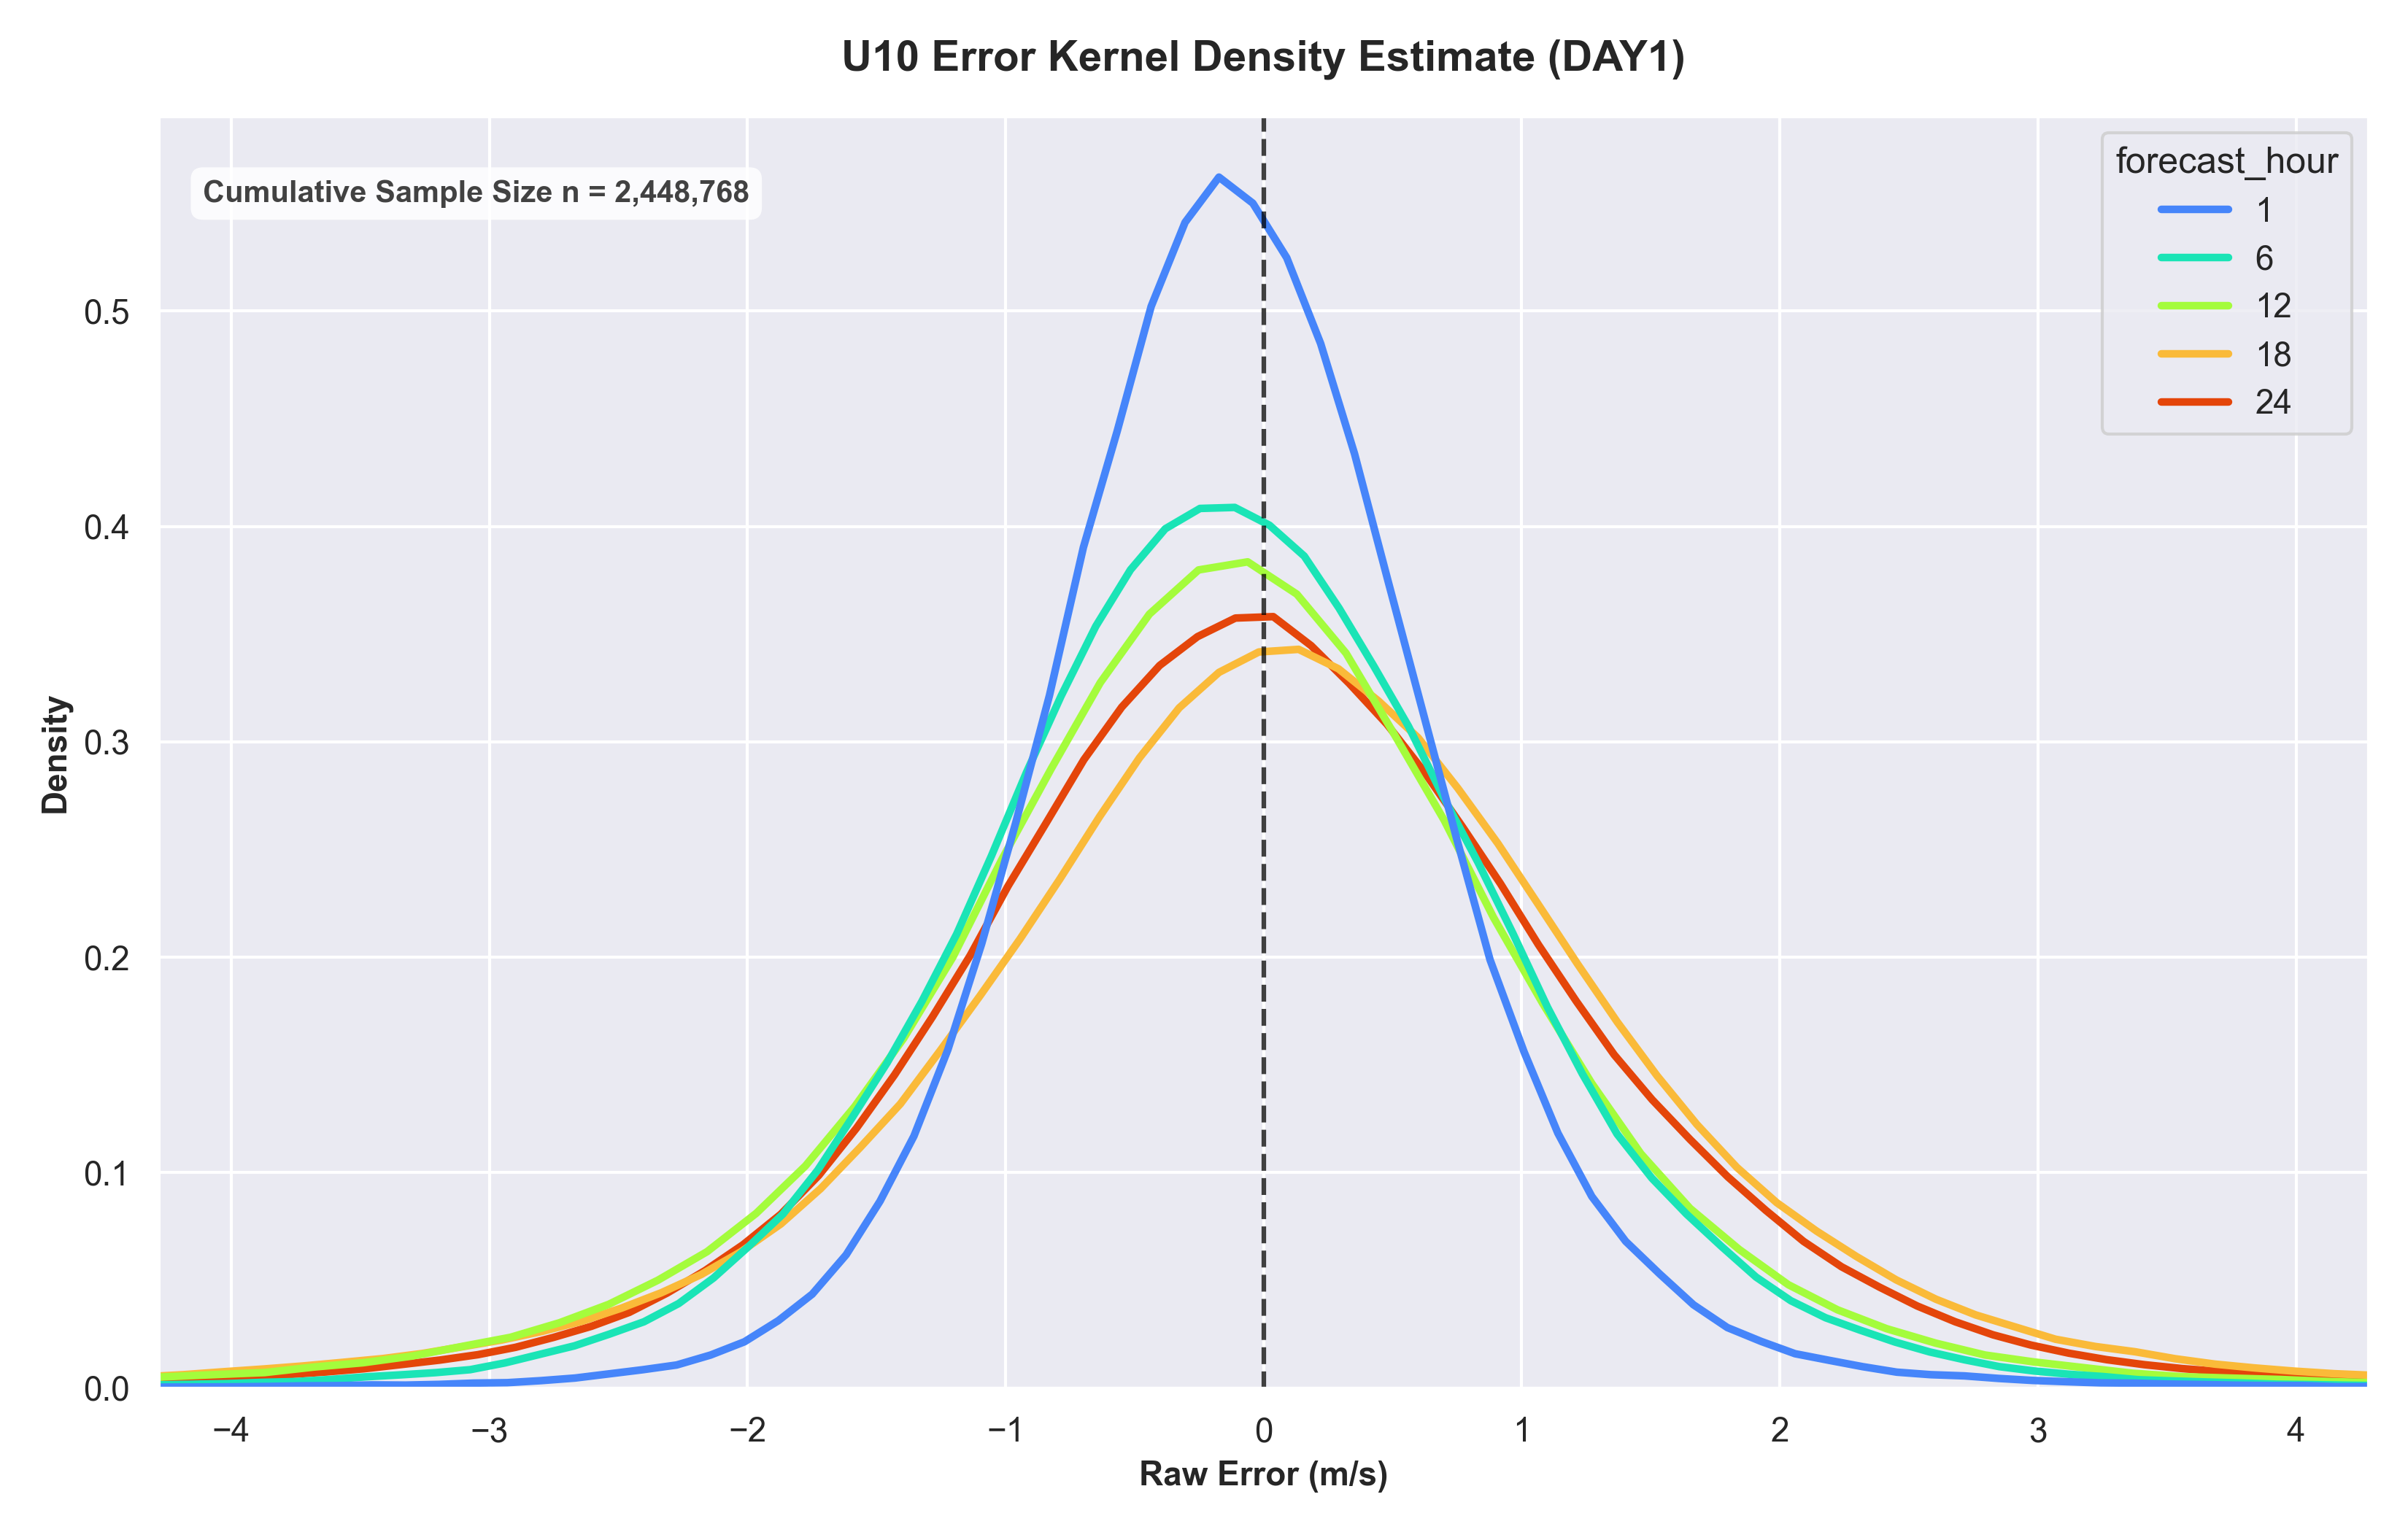
\includegraphics[width=0.49\textwidth]{figures/KDE_GRAPHS_RAW/u10_kde_day1.png}\hfill
  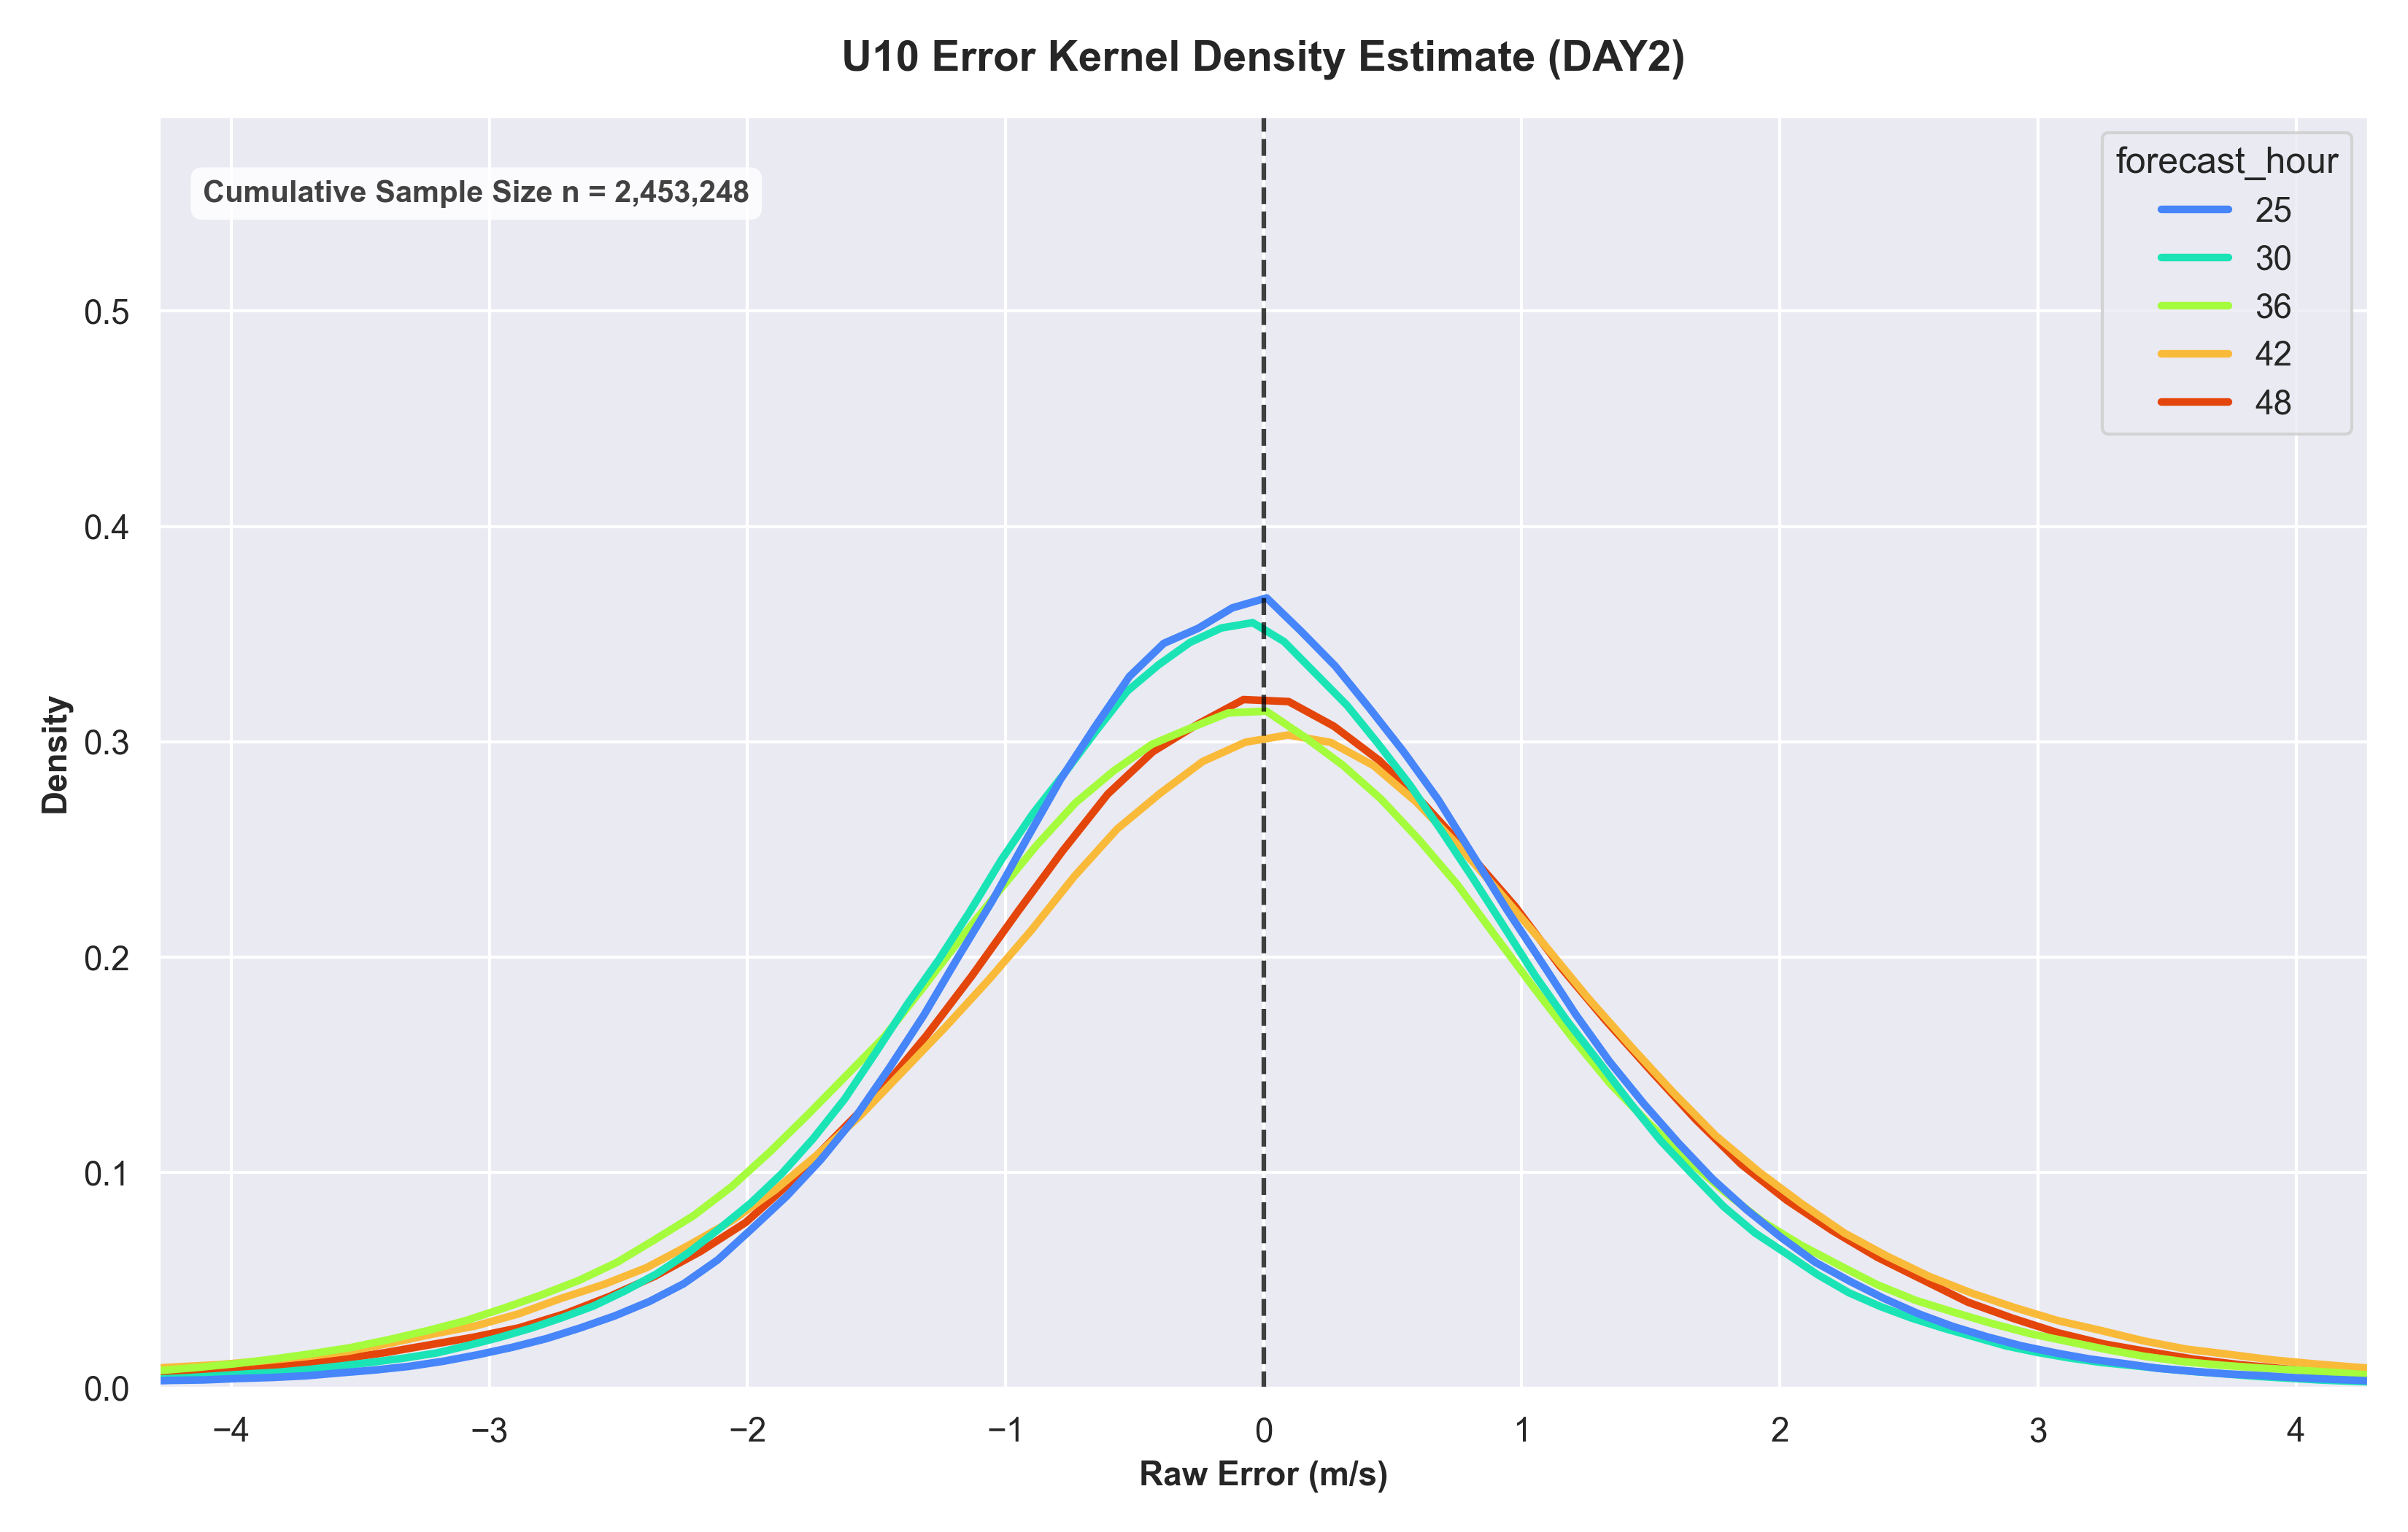
\includegraphics[width=0.49\textwidth]{figures/KDE_GRAPHS_RAW/u10_kde_day2.png}
  \caption{Kernel Density Estimation (KDE) of U10 wind component forecast errors for Day 1 (left) and Day 2 (right).}
  \label{fig:kde_u10}
\end{figure}

\begin{figure}[H]
  \centering
  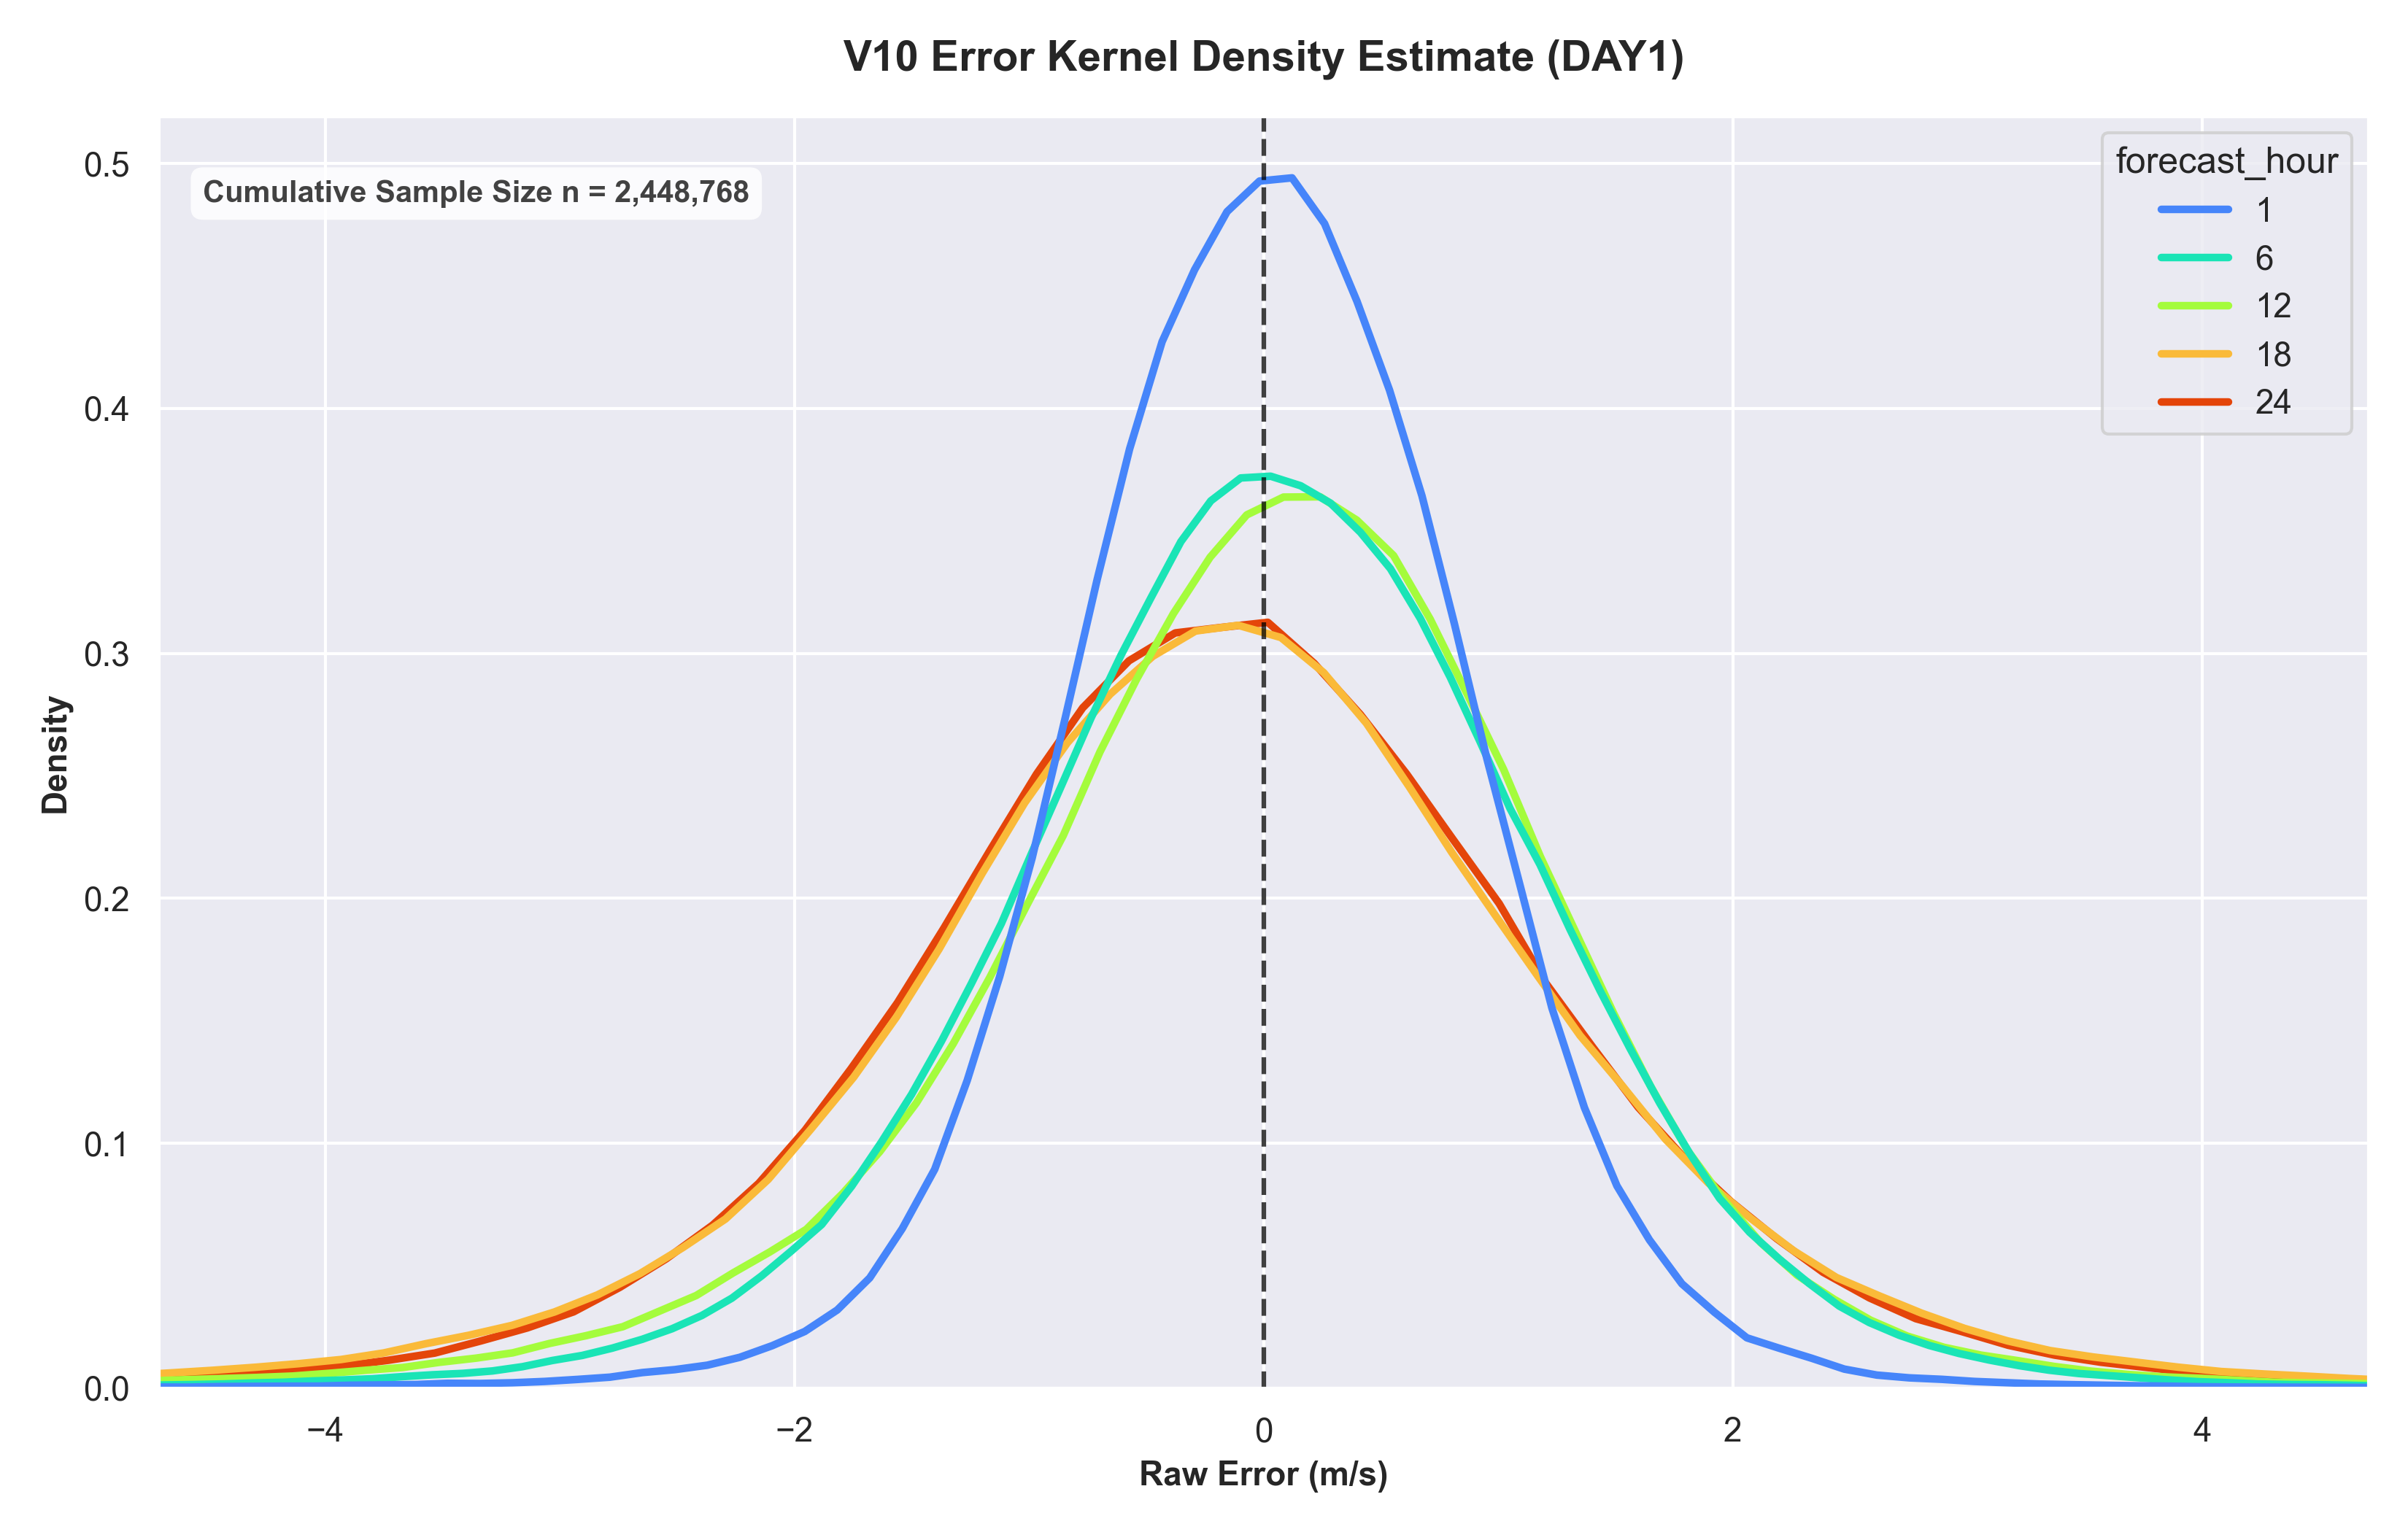
\includegraphics[width=0.49\textwidth]{figures/KDE_GRAPHS_RAW/v10_kde_day1.png}\hfill
  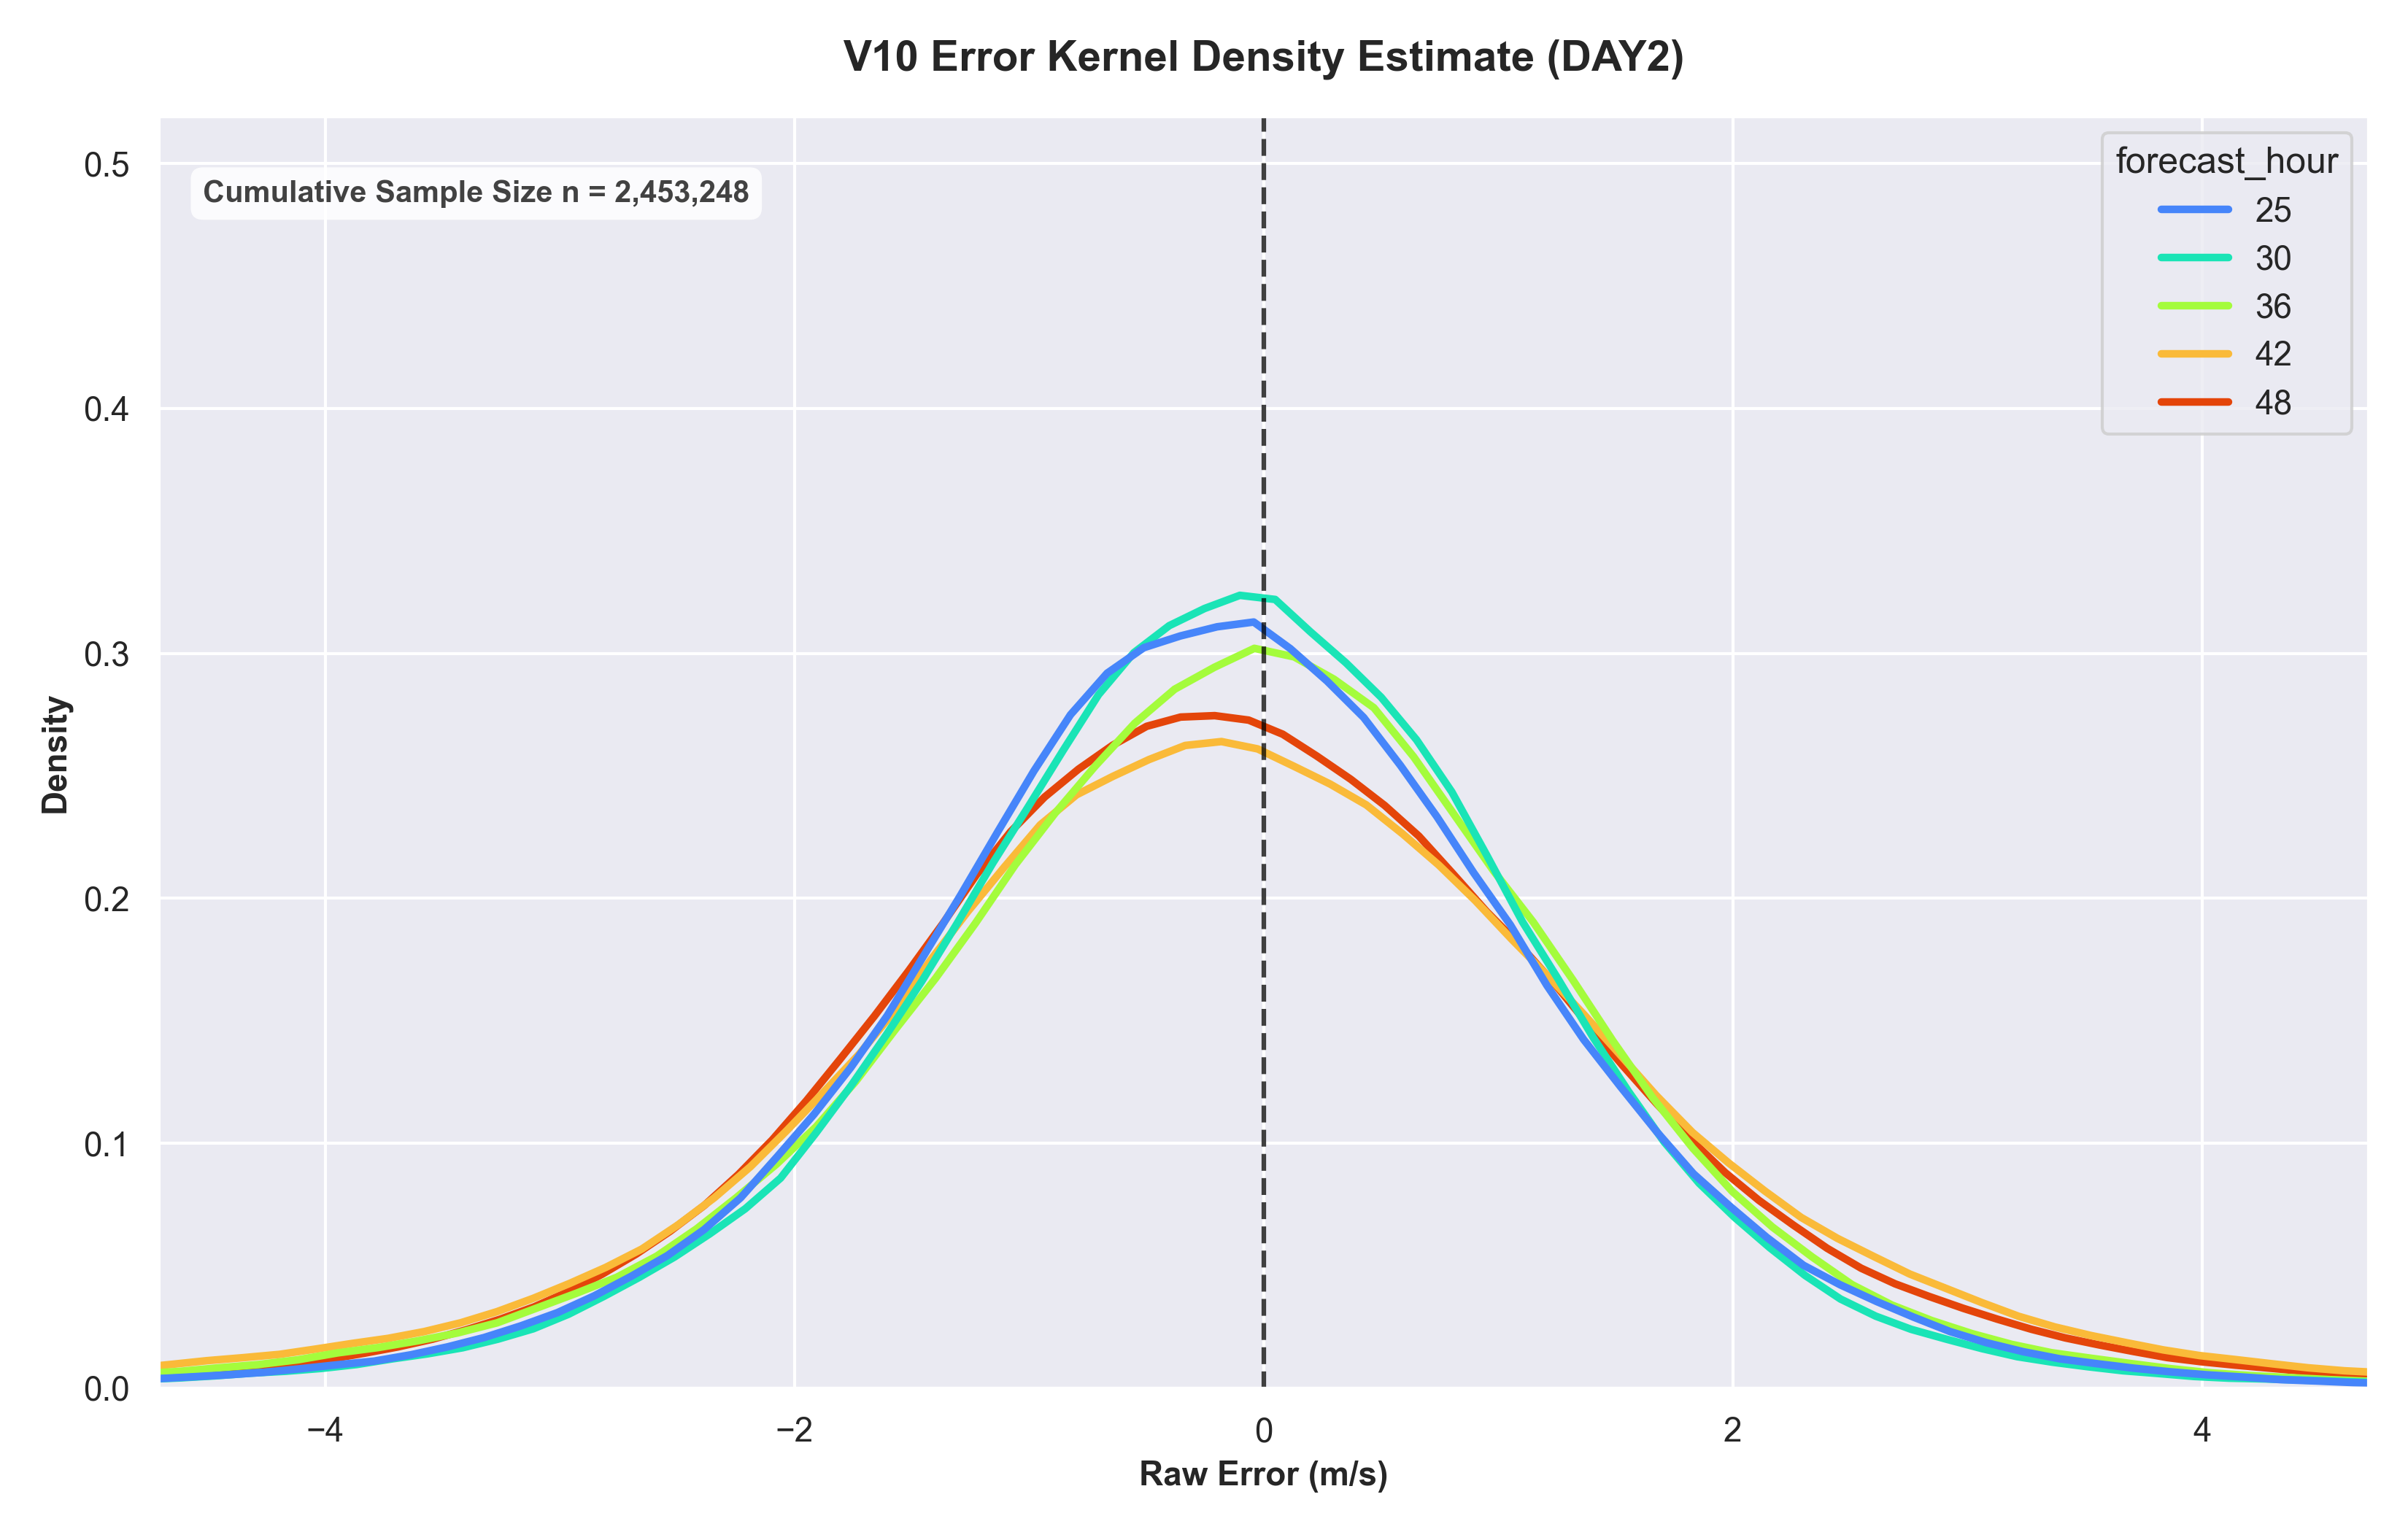
\includegraphics[width=0.49\textwidth]{figures/KDE_GRAPHS_RAW/v10_kde_day2.png}
  \caption{Kernel Density Estimation (KDE) of V10 wind component forecast errors for Day 1 (left) and Day 2 (right).}
  \label{fig:kde_v10}
\end{figure}

\begin{figure}[H]
  \centering
  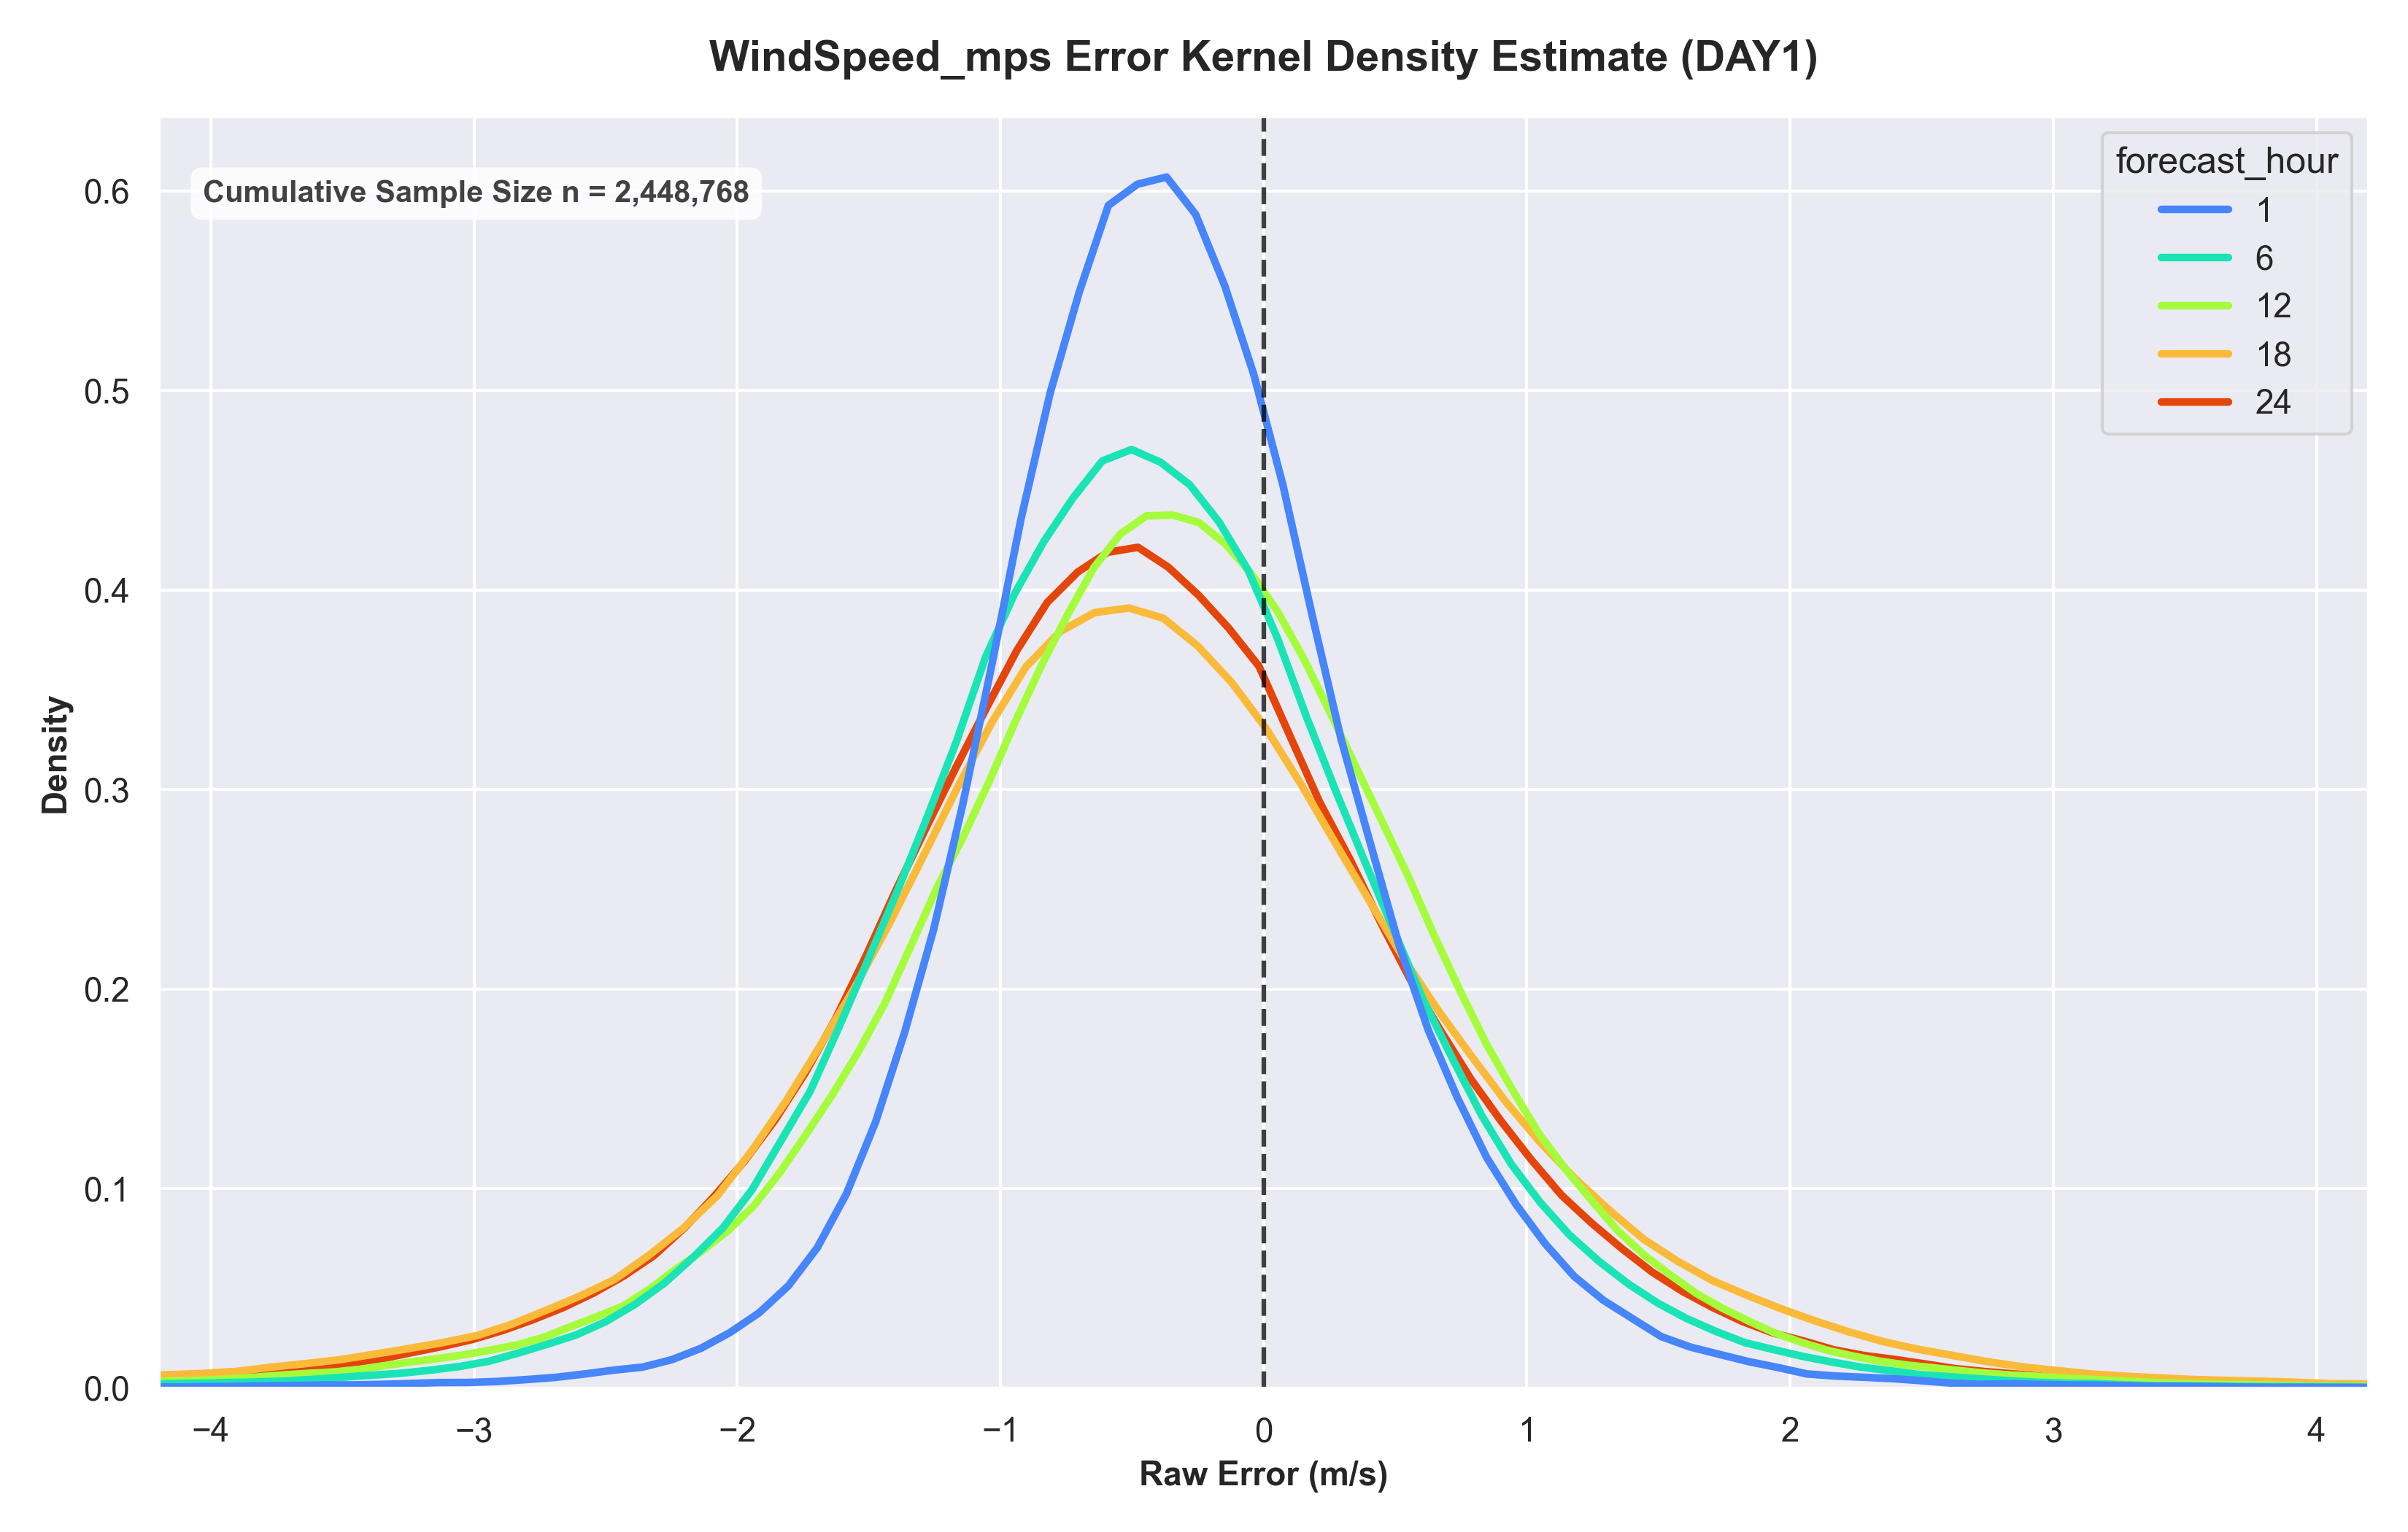
\includegraphics[width=0.49\textwidth]{figures/KDE_GRAPHS_RAW/windspeed_mps_kde_day1.png}\hfill
  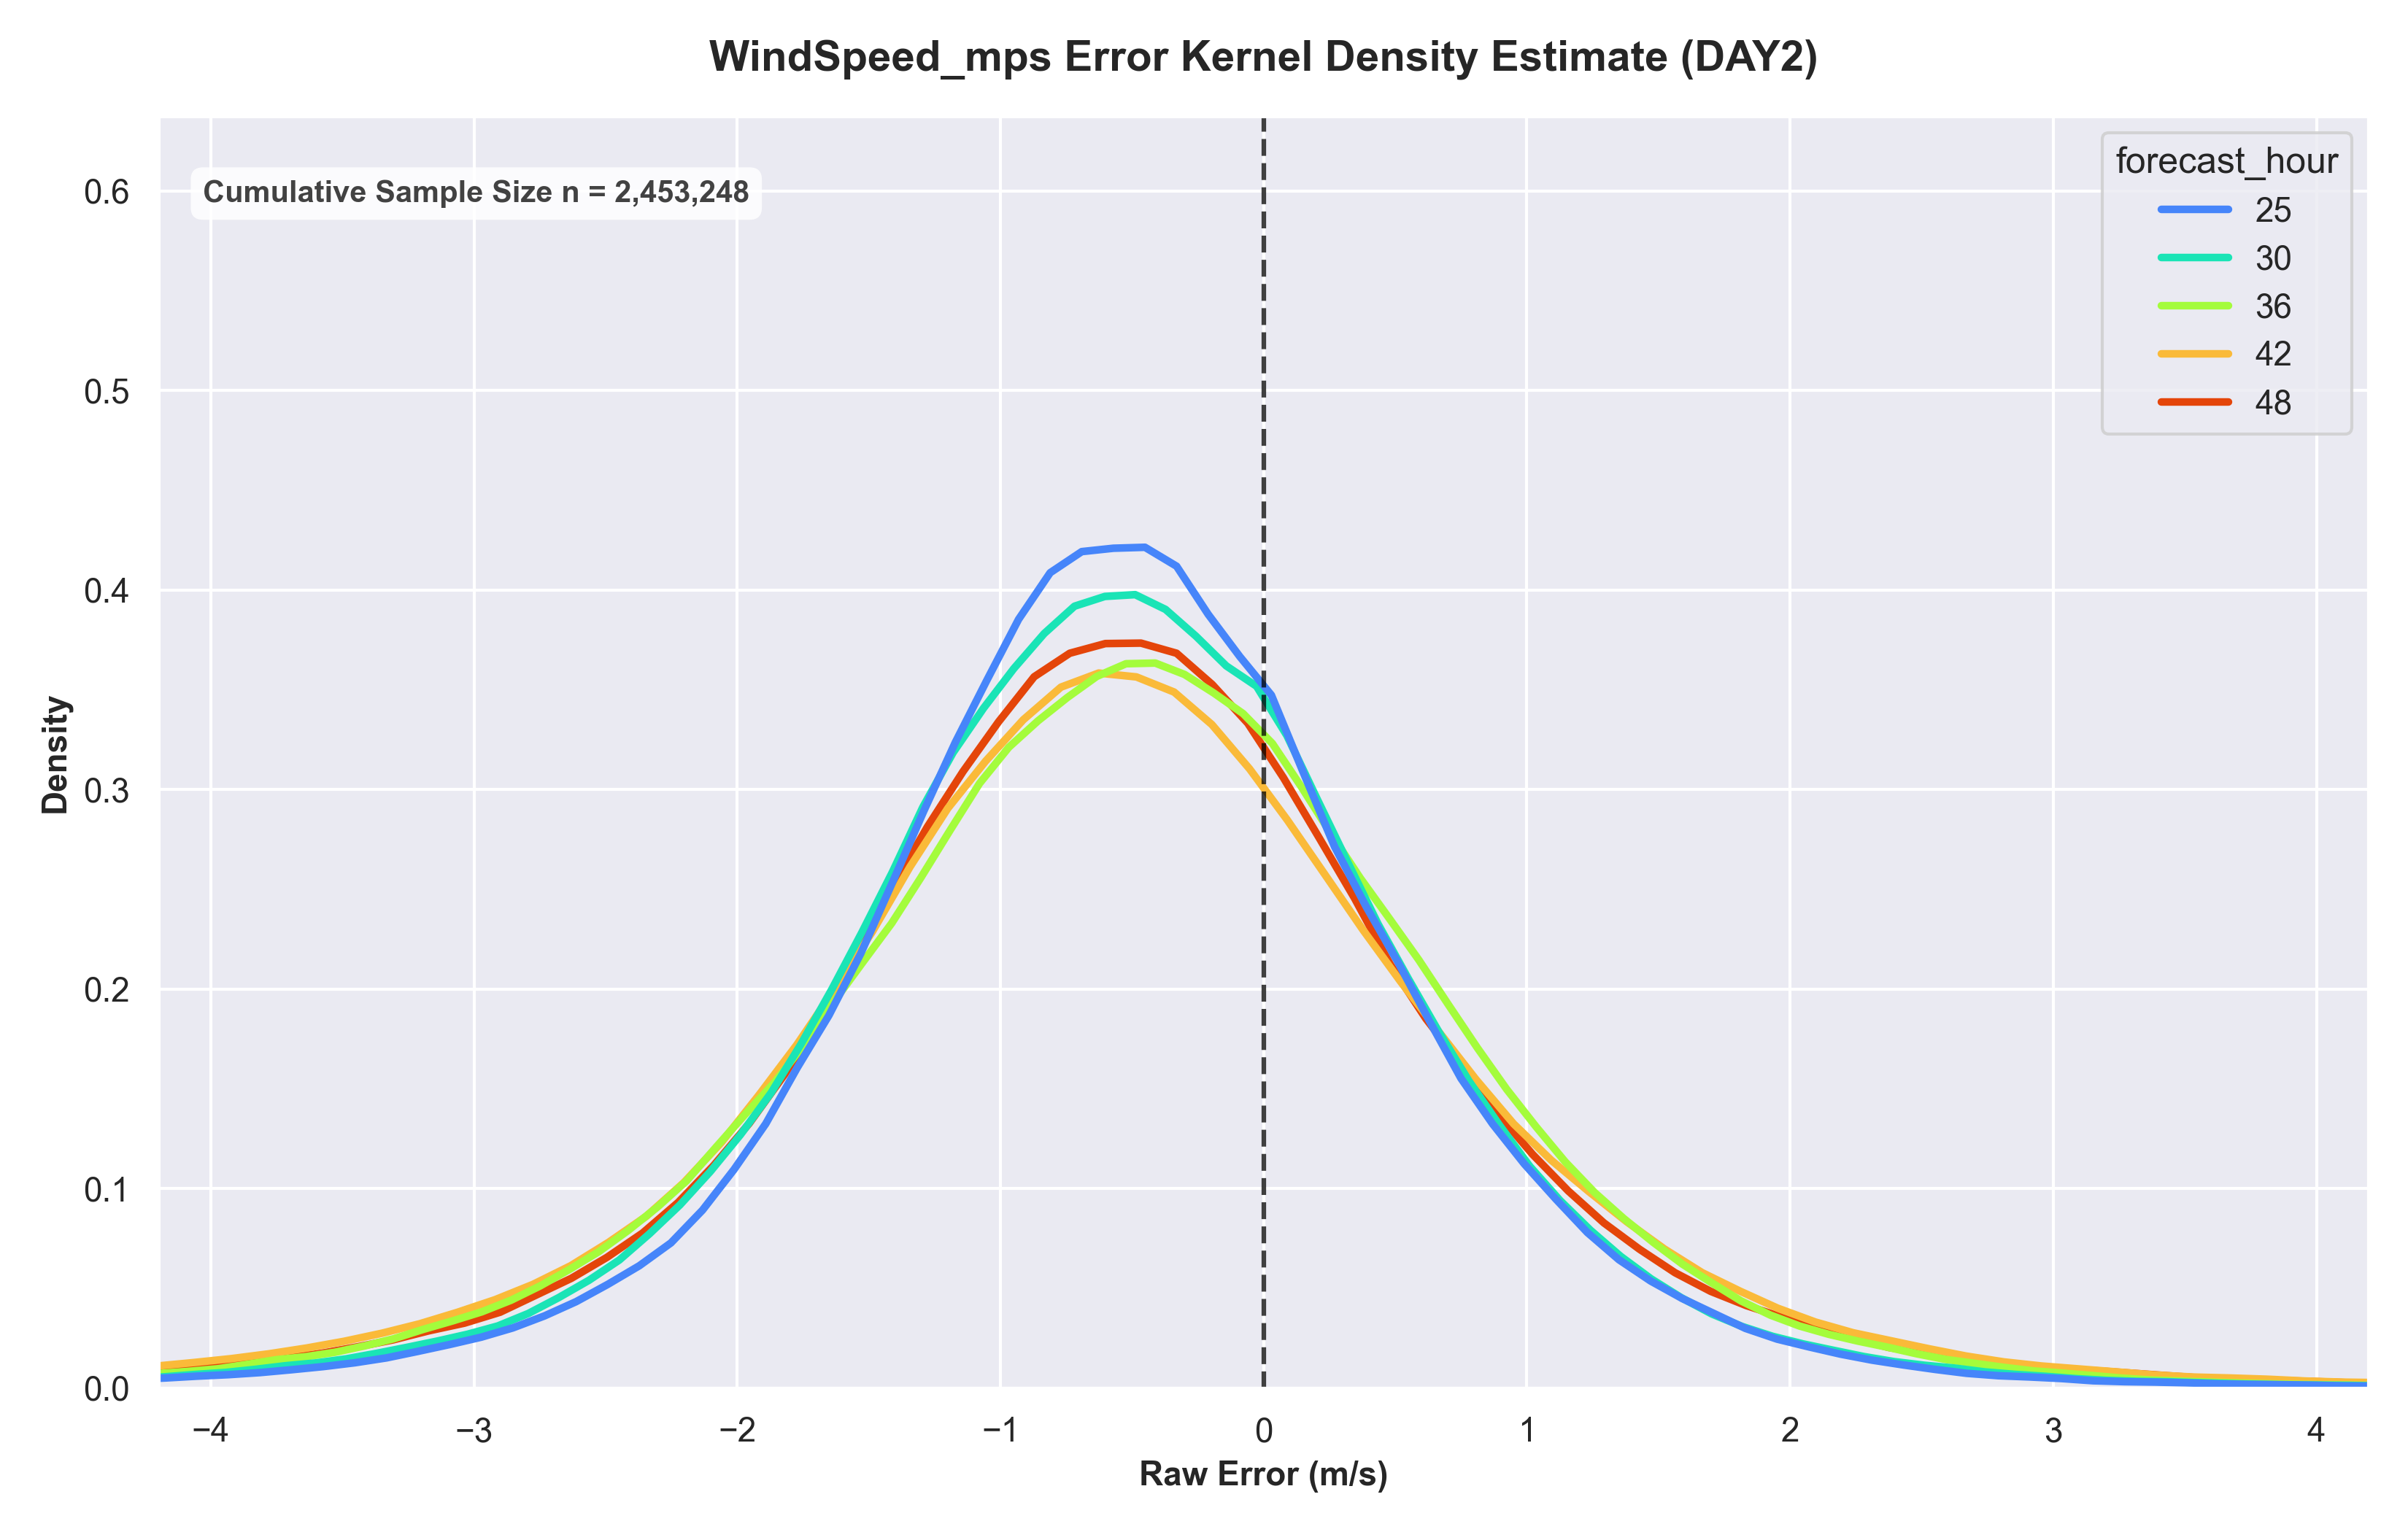
\includegraphics[width=0.49\textwidth]{figures/KDE_GRAPHS_RAW/windspeed_mps_kde_day2.png}
  \caption{Kernel Density Estimation (KDE) of Wind Speed forecast errors for Day 1 (left) and Day 2 (right).}
  \label{fig:kde_windspeed}
\end{figure}

\begin{figure}[H]
  \centering
  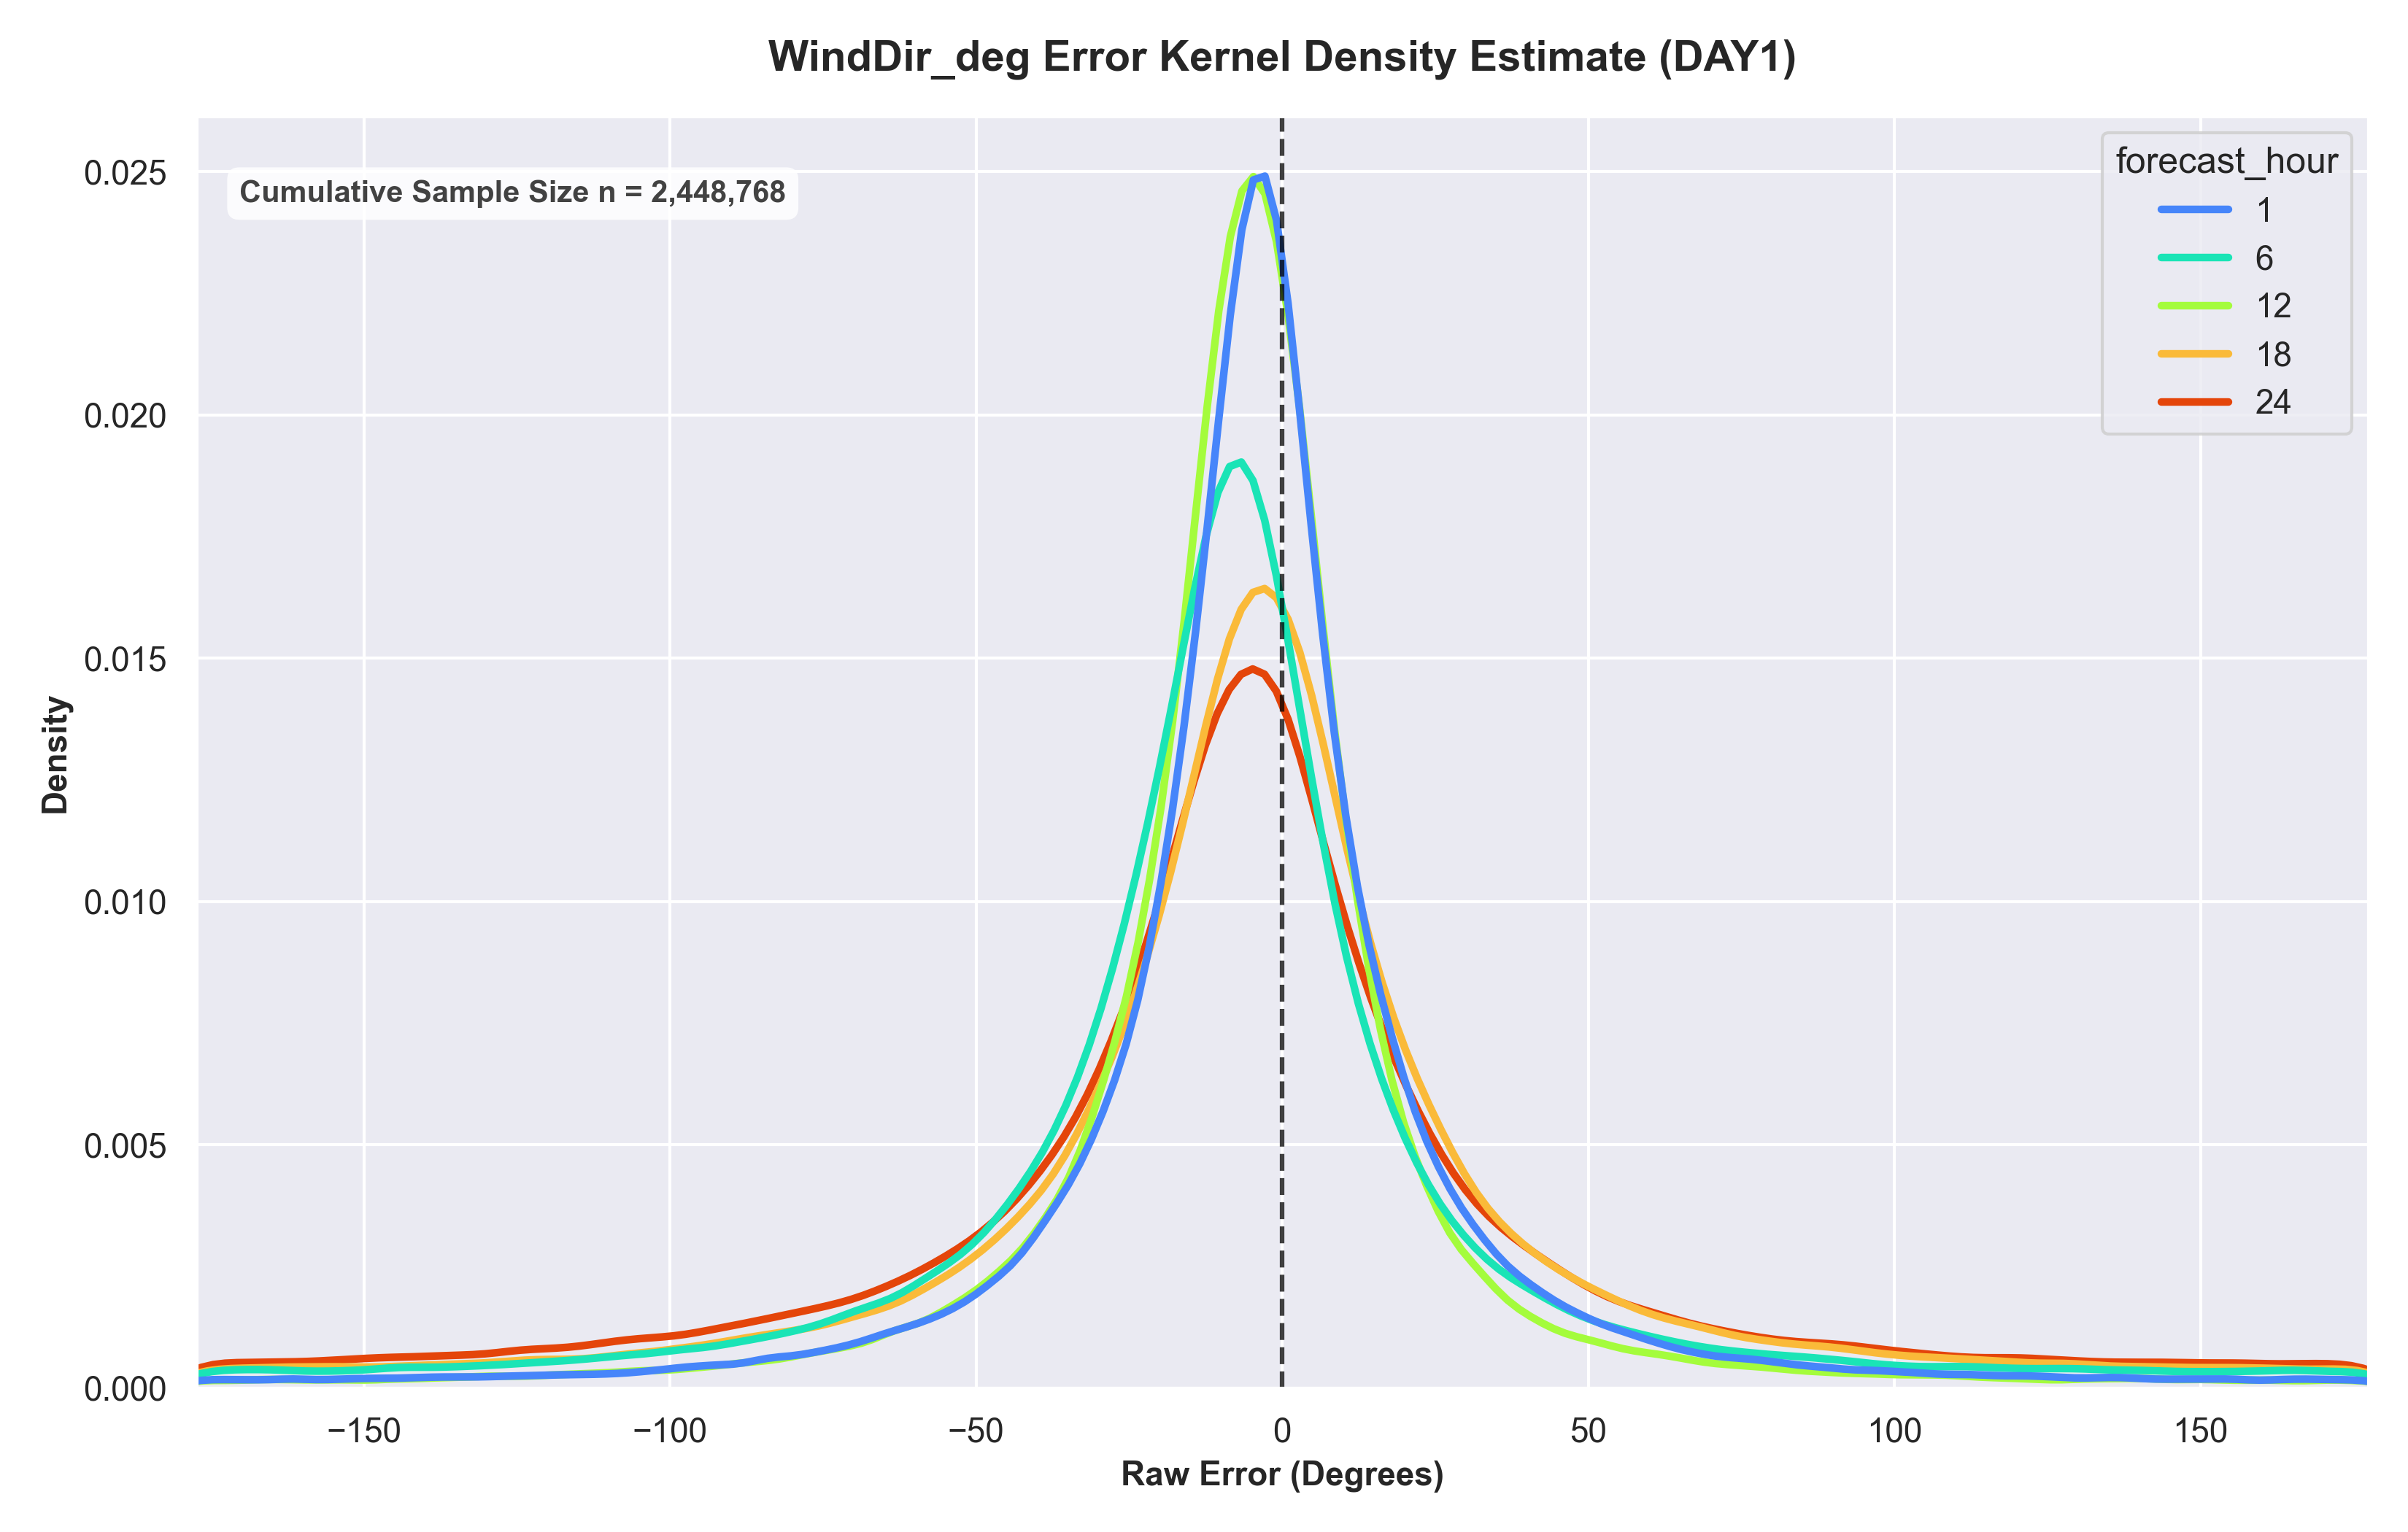
\includegraphics[width=0.49\textwidth]{figures/KDE_GRAPHS_RAW/winddir_deg_kde_day1.png}\hfill
  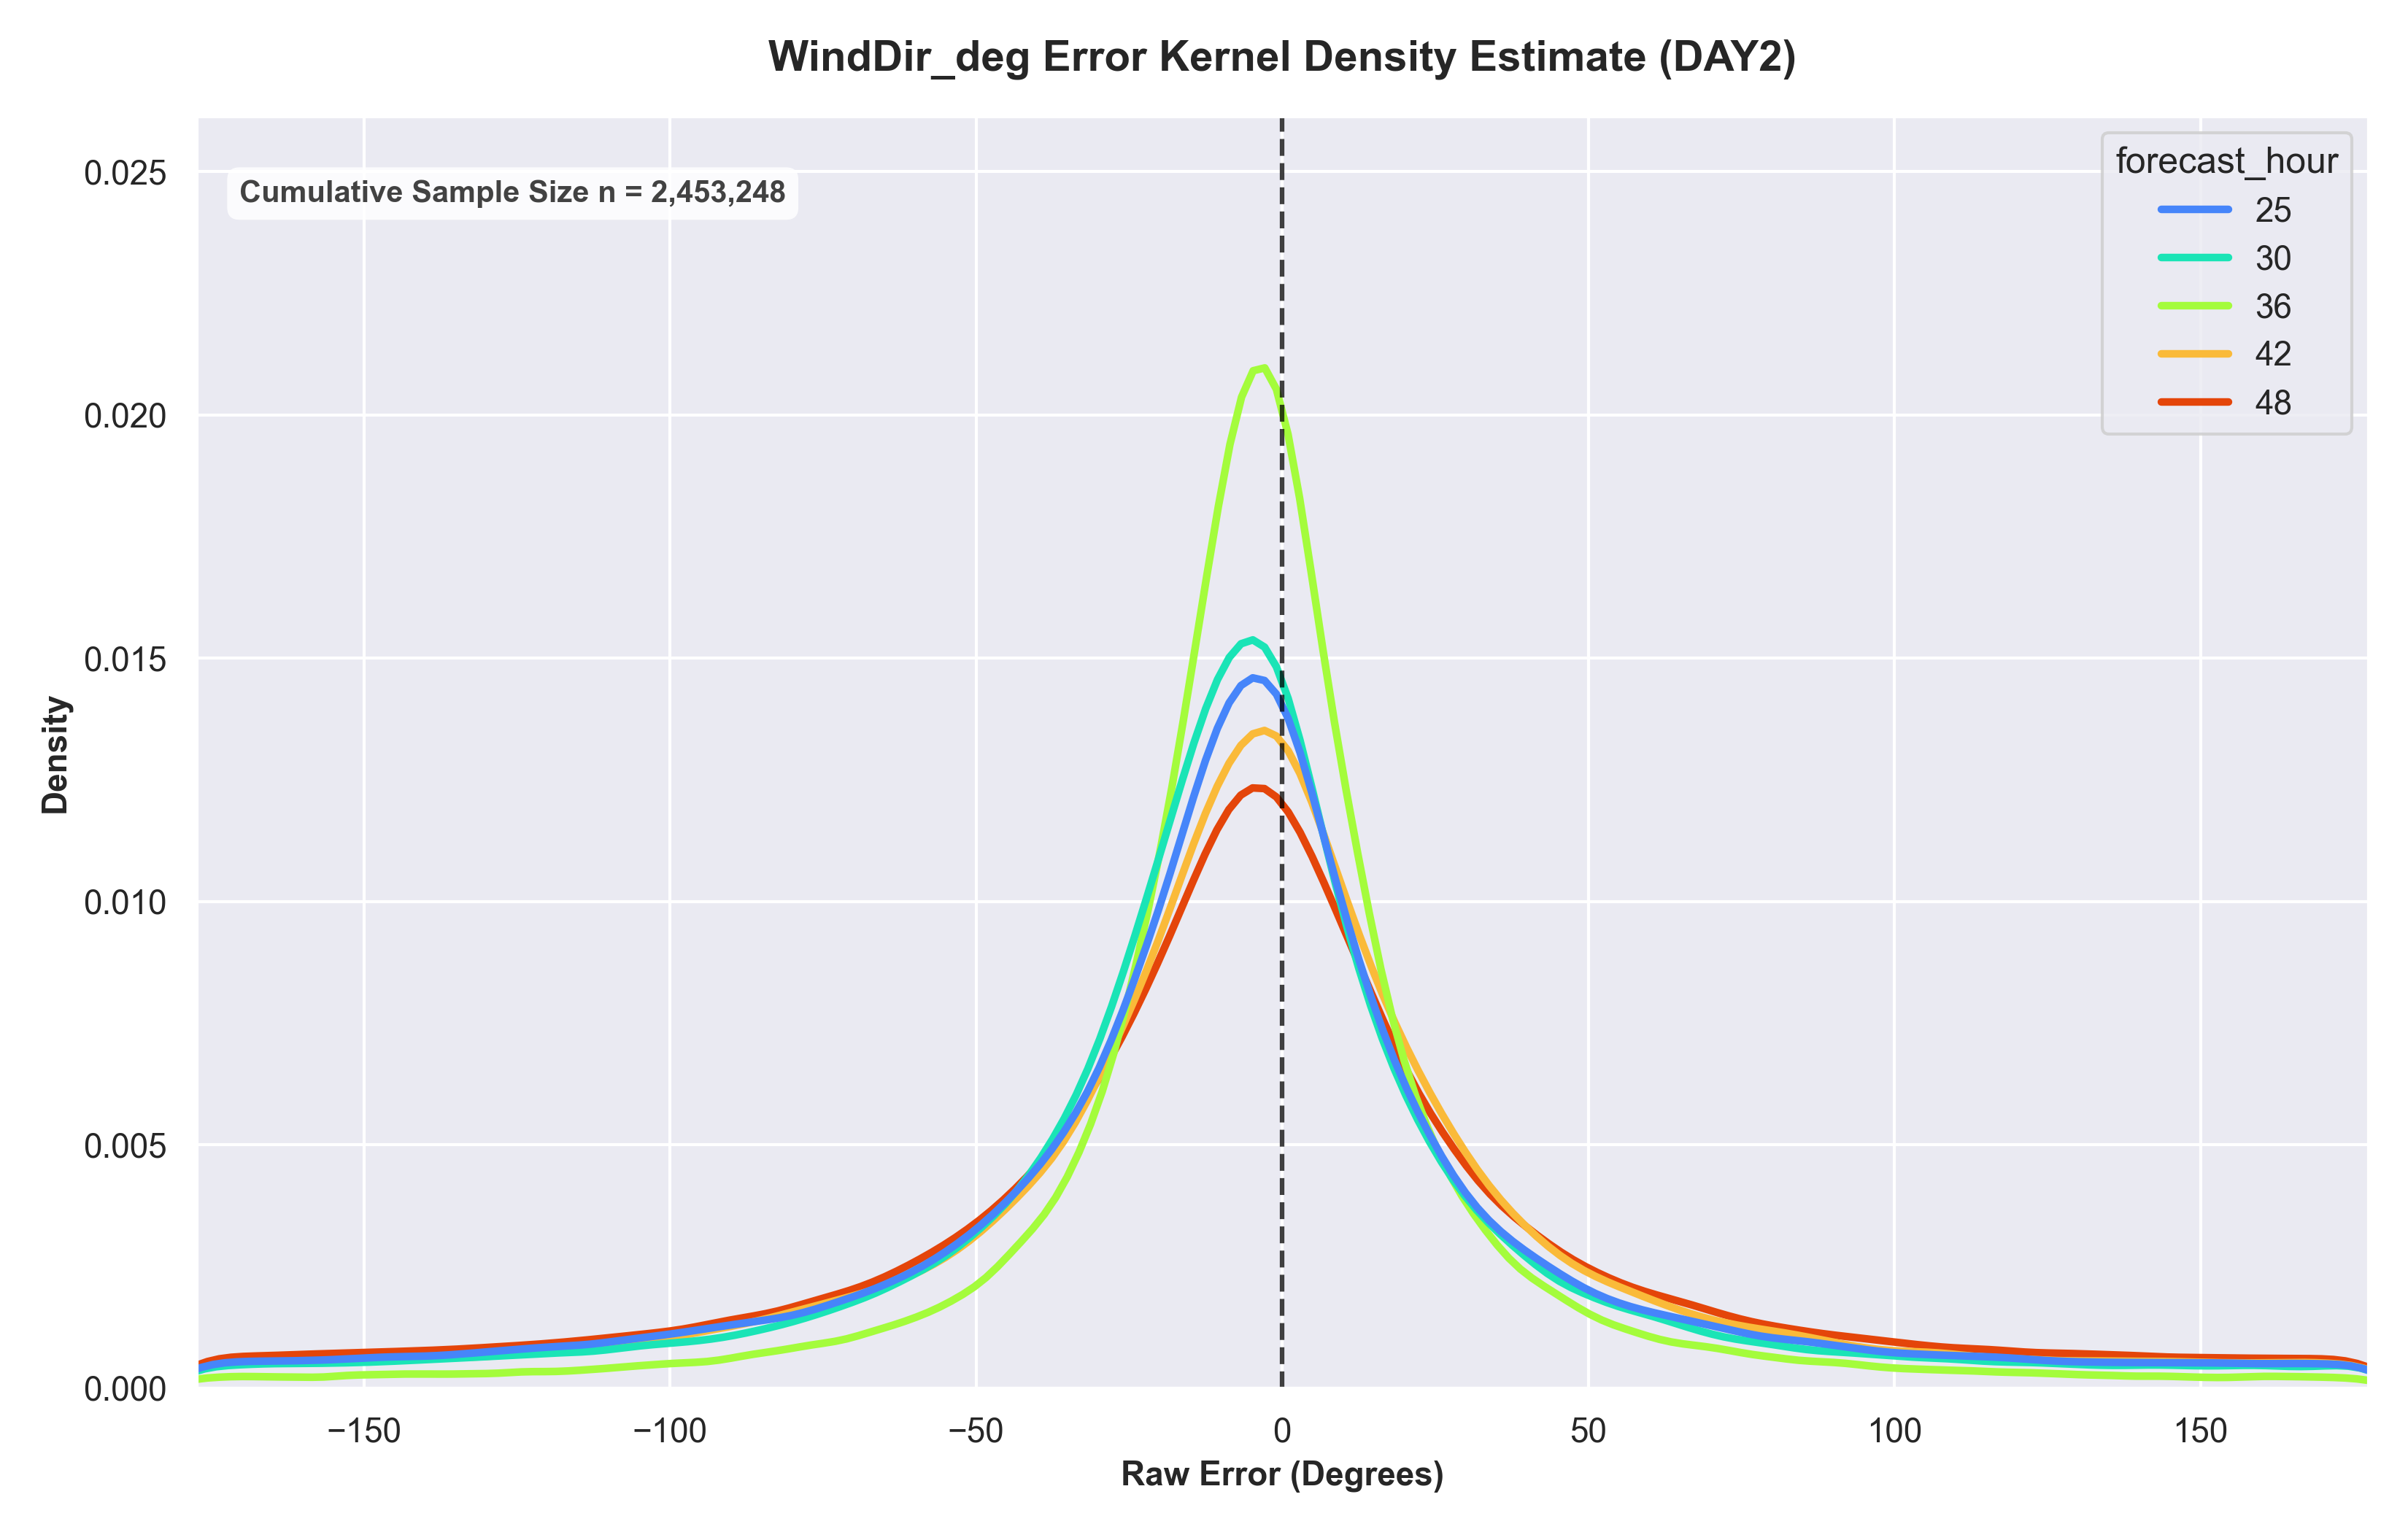
\includegraphics[width=0.49\textwidth]{figures/KDE_GRAPHS_RAW/winddir_deg_kde_day2.png}
  \caption{Kernel Density Estimation (KDE) of Wind Direction forecast errors for Day 1 (left) and Day 2 (right).}
  \label{fig:kde_winddir}
\end{figure}

\subsection{Q2 — Forecast Error vs. Lead Time}

\begin{figure}[H]
  \centering
  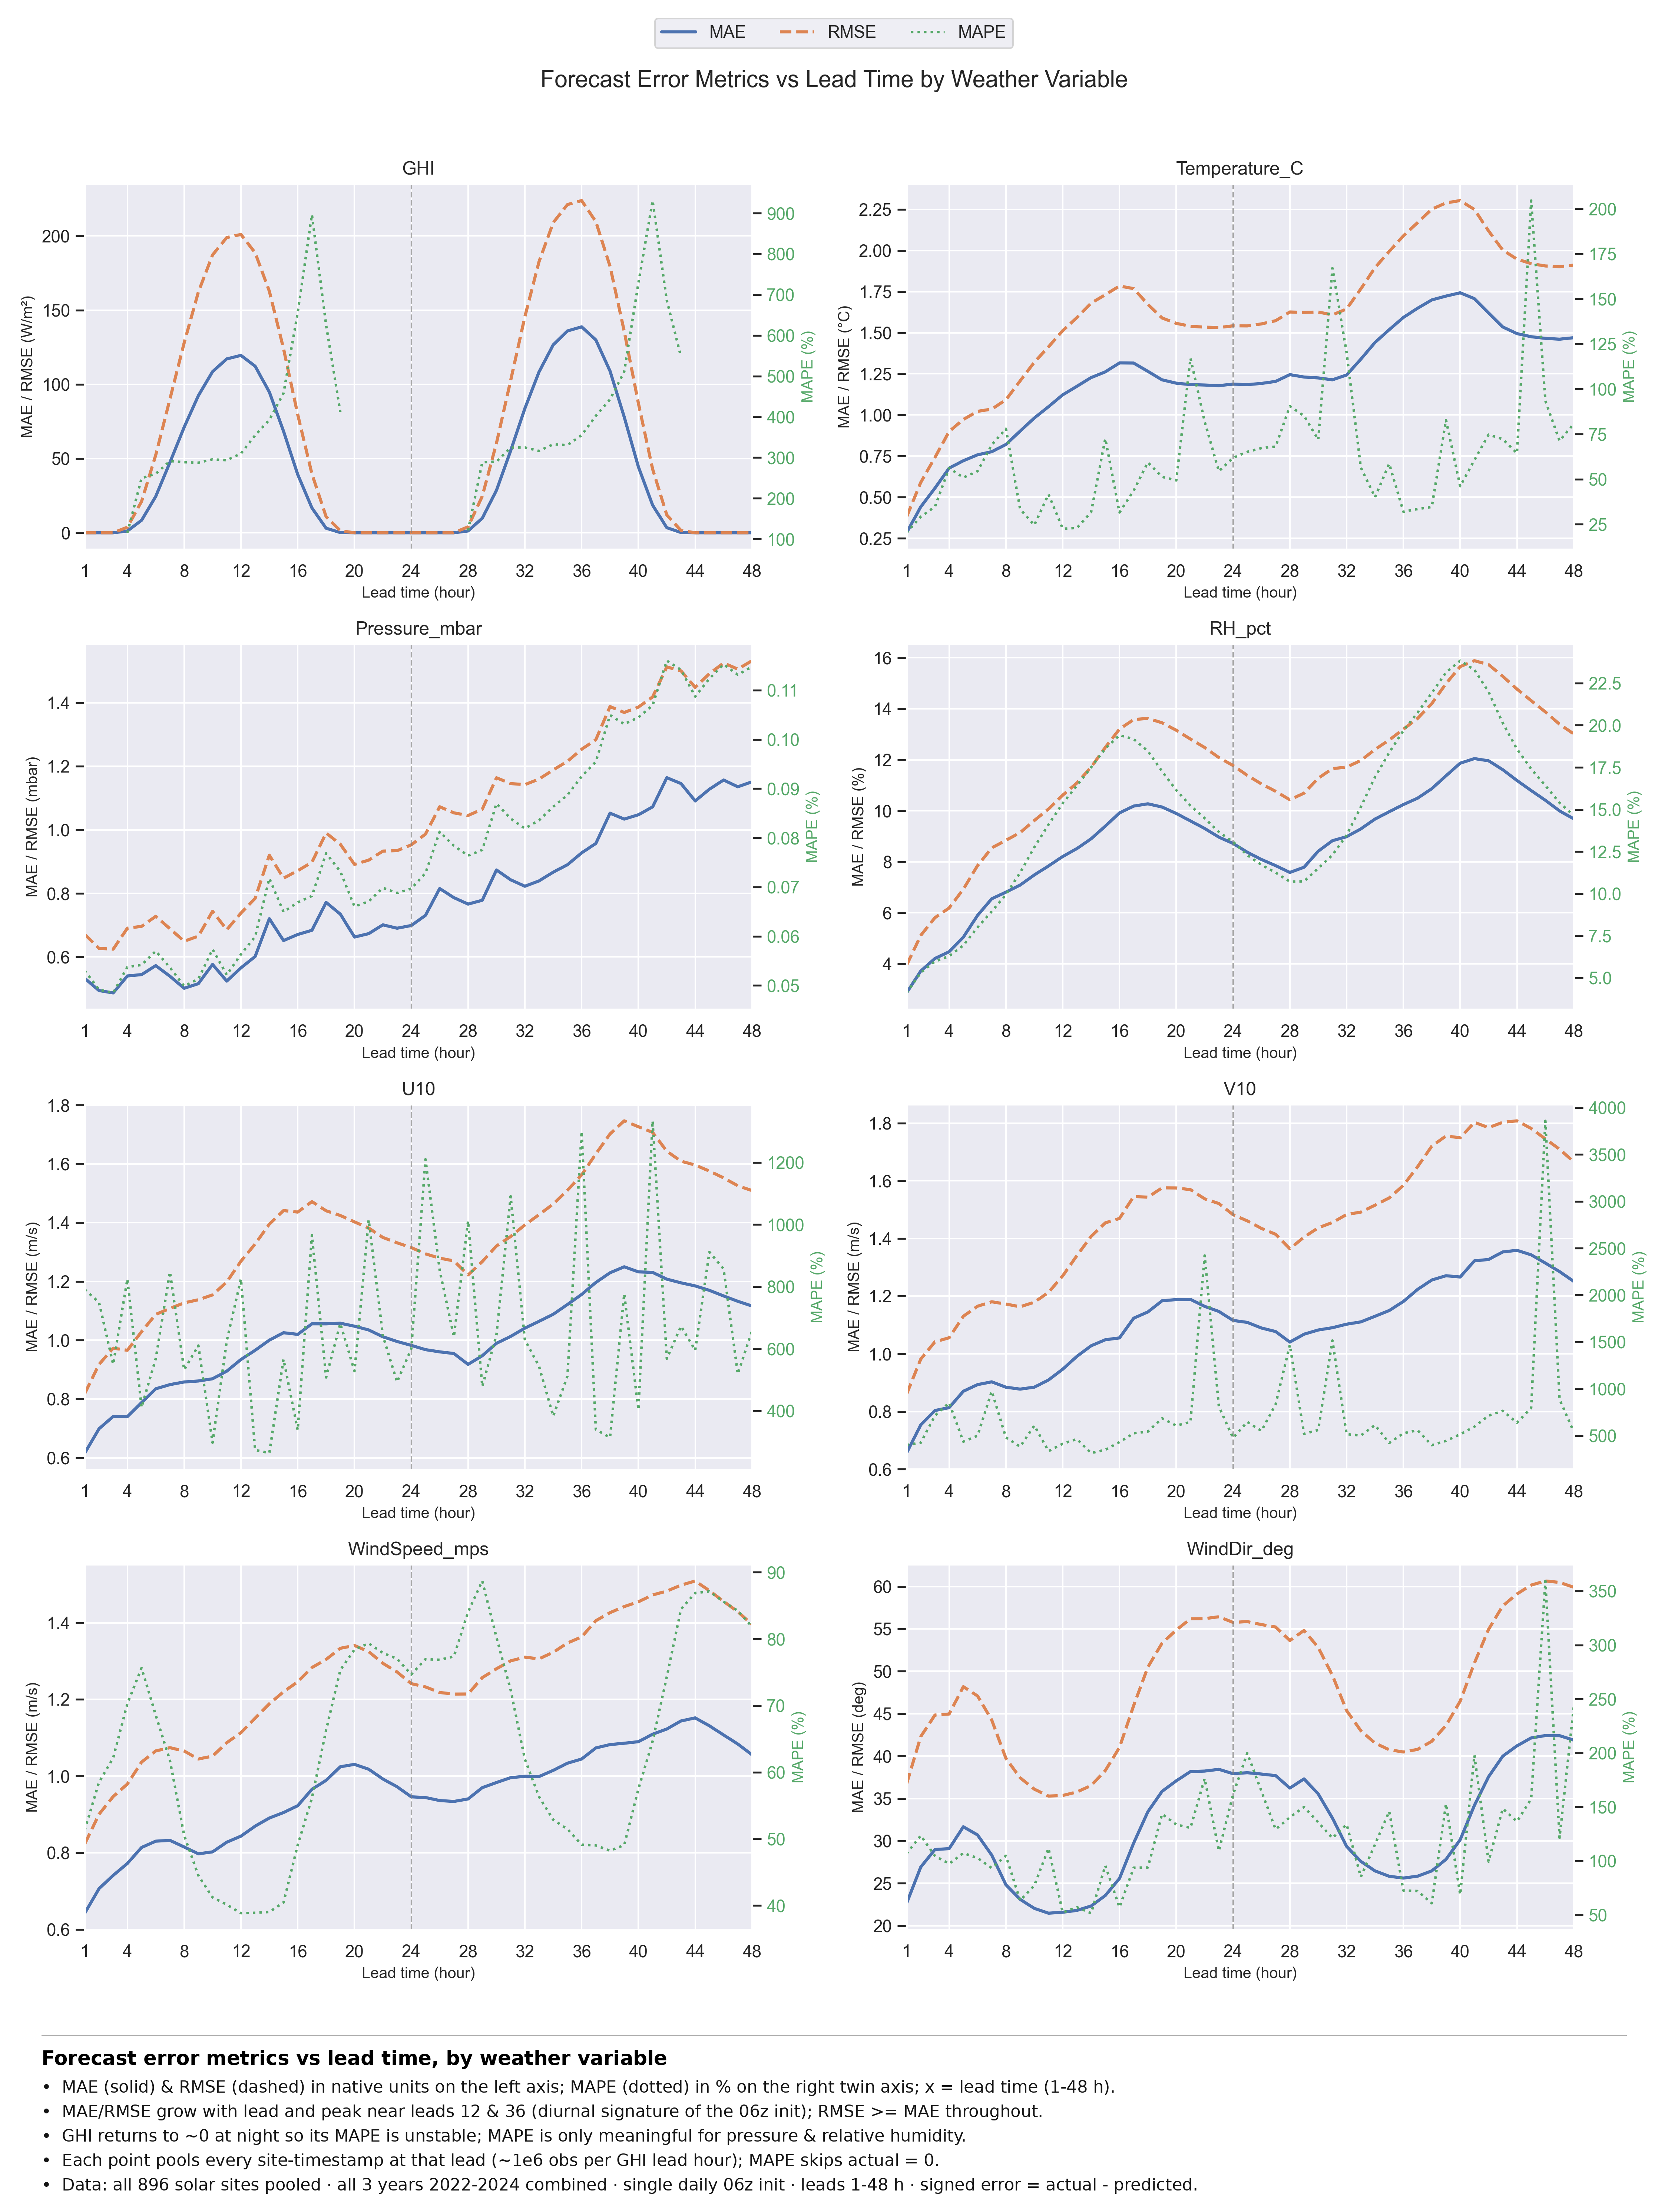
\includegraphics[width=\textwidth]{figures/Q2/error_by_lead_time_solar.png}
  \caption{Complete (all-variable) version of forecast error metrics versus lead time.}
  \label{fig:app_leadtime}
\end{figure}

\begin{figure}[H]
  \centering
  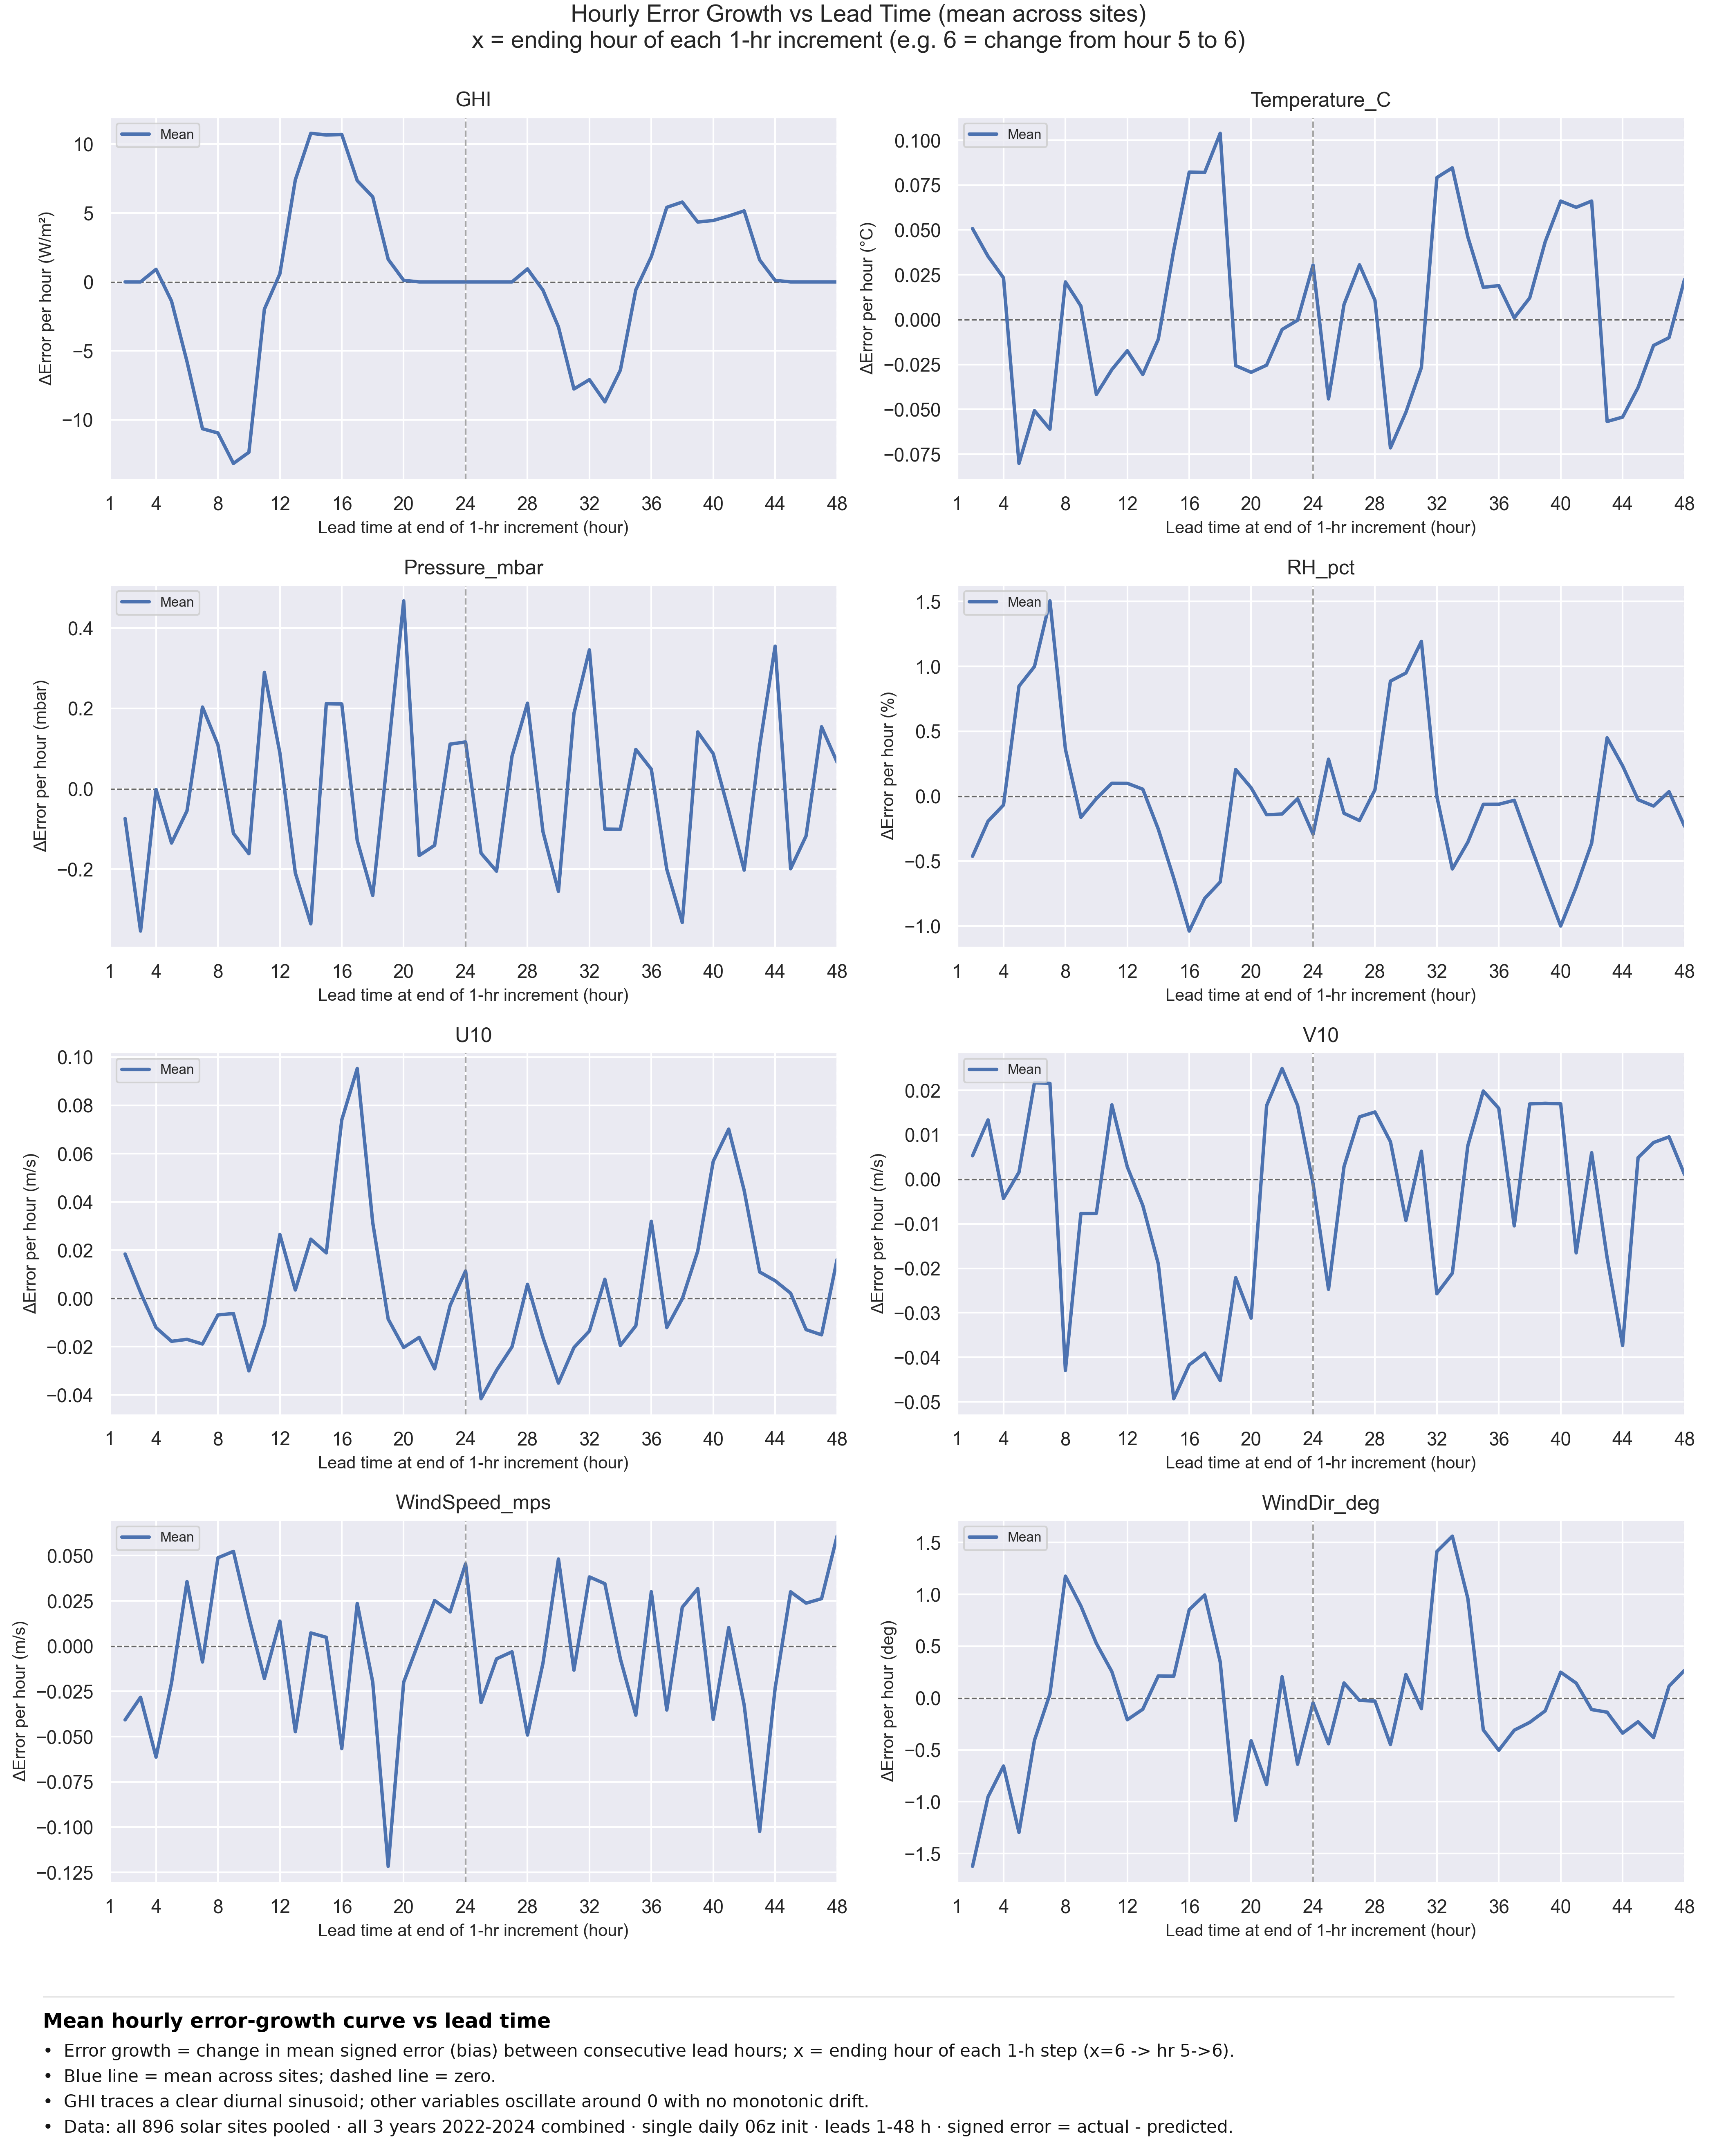
\includegraphics[width=\textwidth]{figures/Q2/error_growth_curves.png}
  \caption{Complete (all-variable) version of the fleet-mean hourly error-growth curves.}
  \label{fig:app_growthcurves}
\end{figure}

\begin{figure}[H]
  \centering
  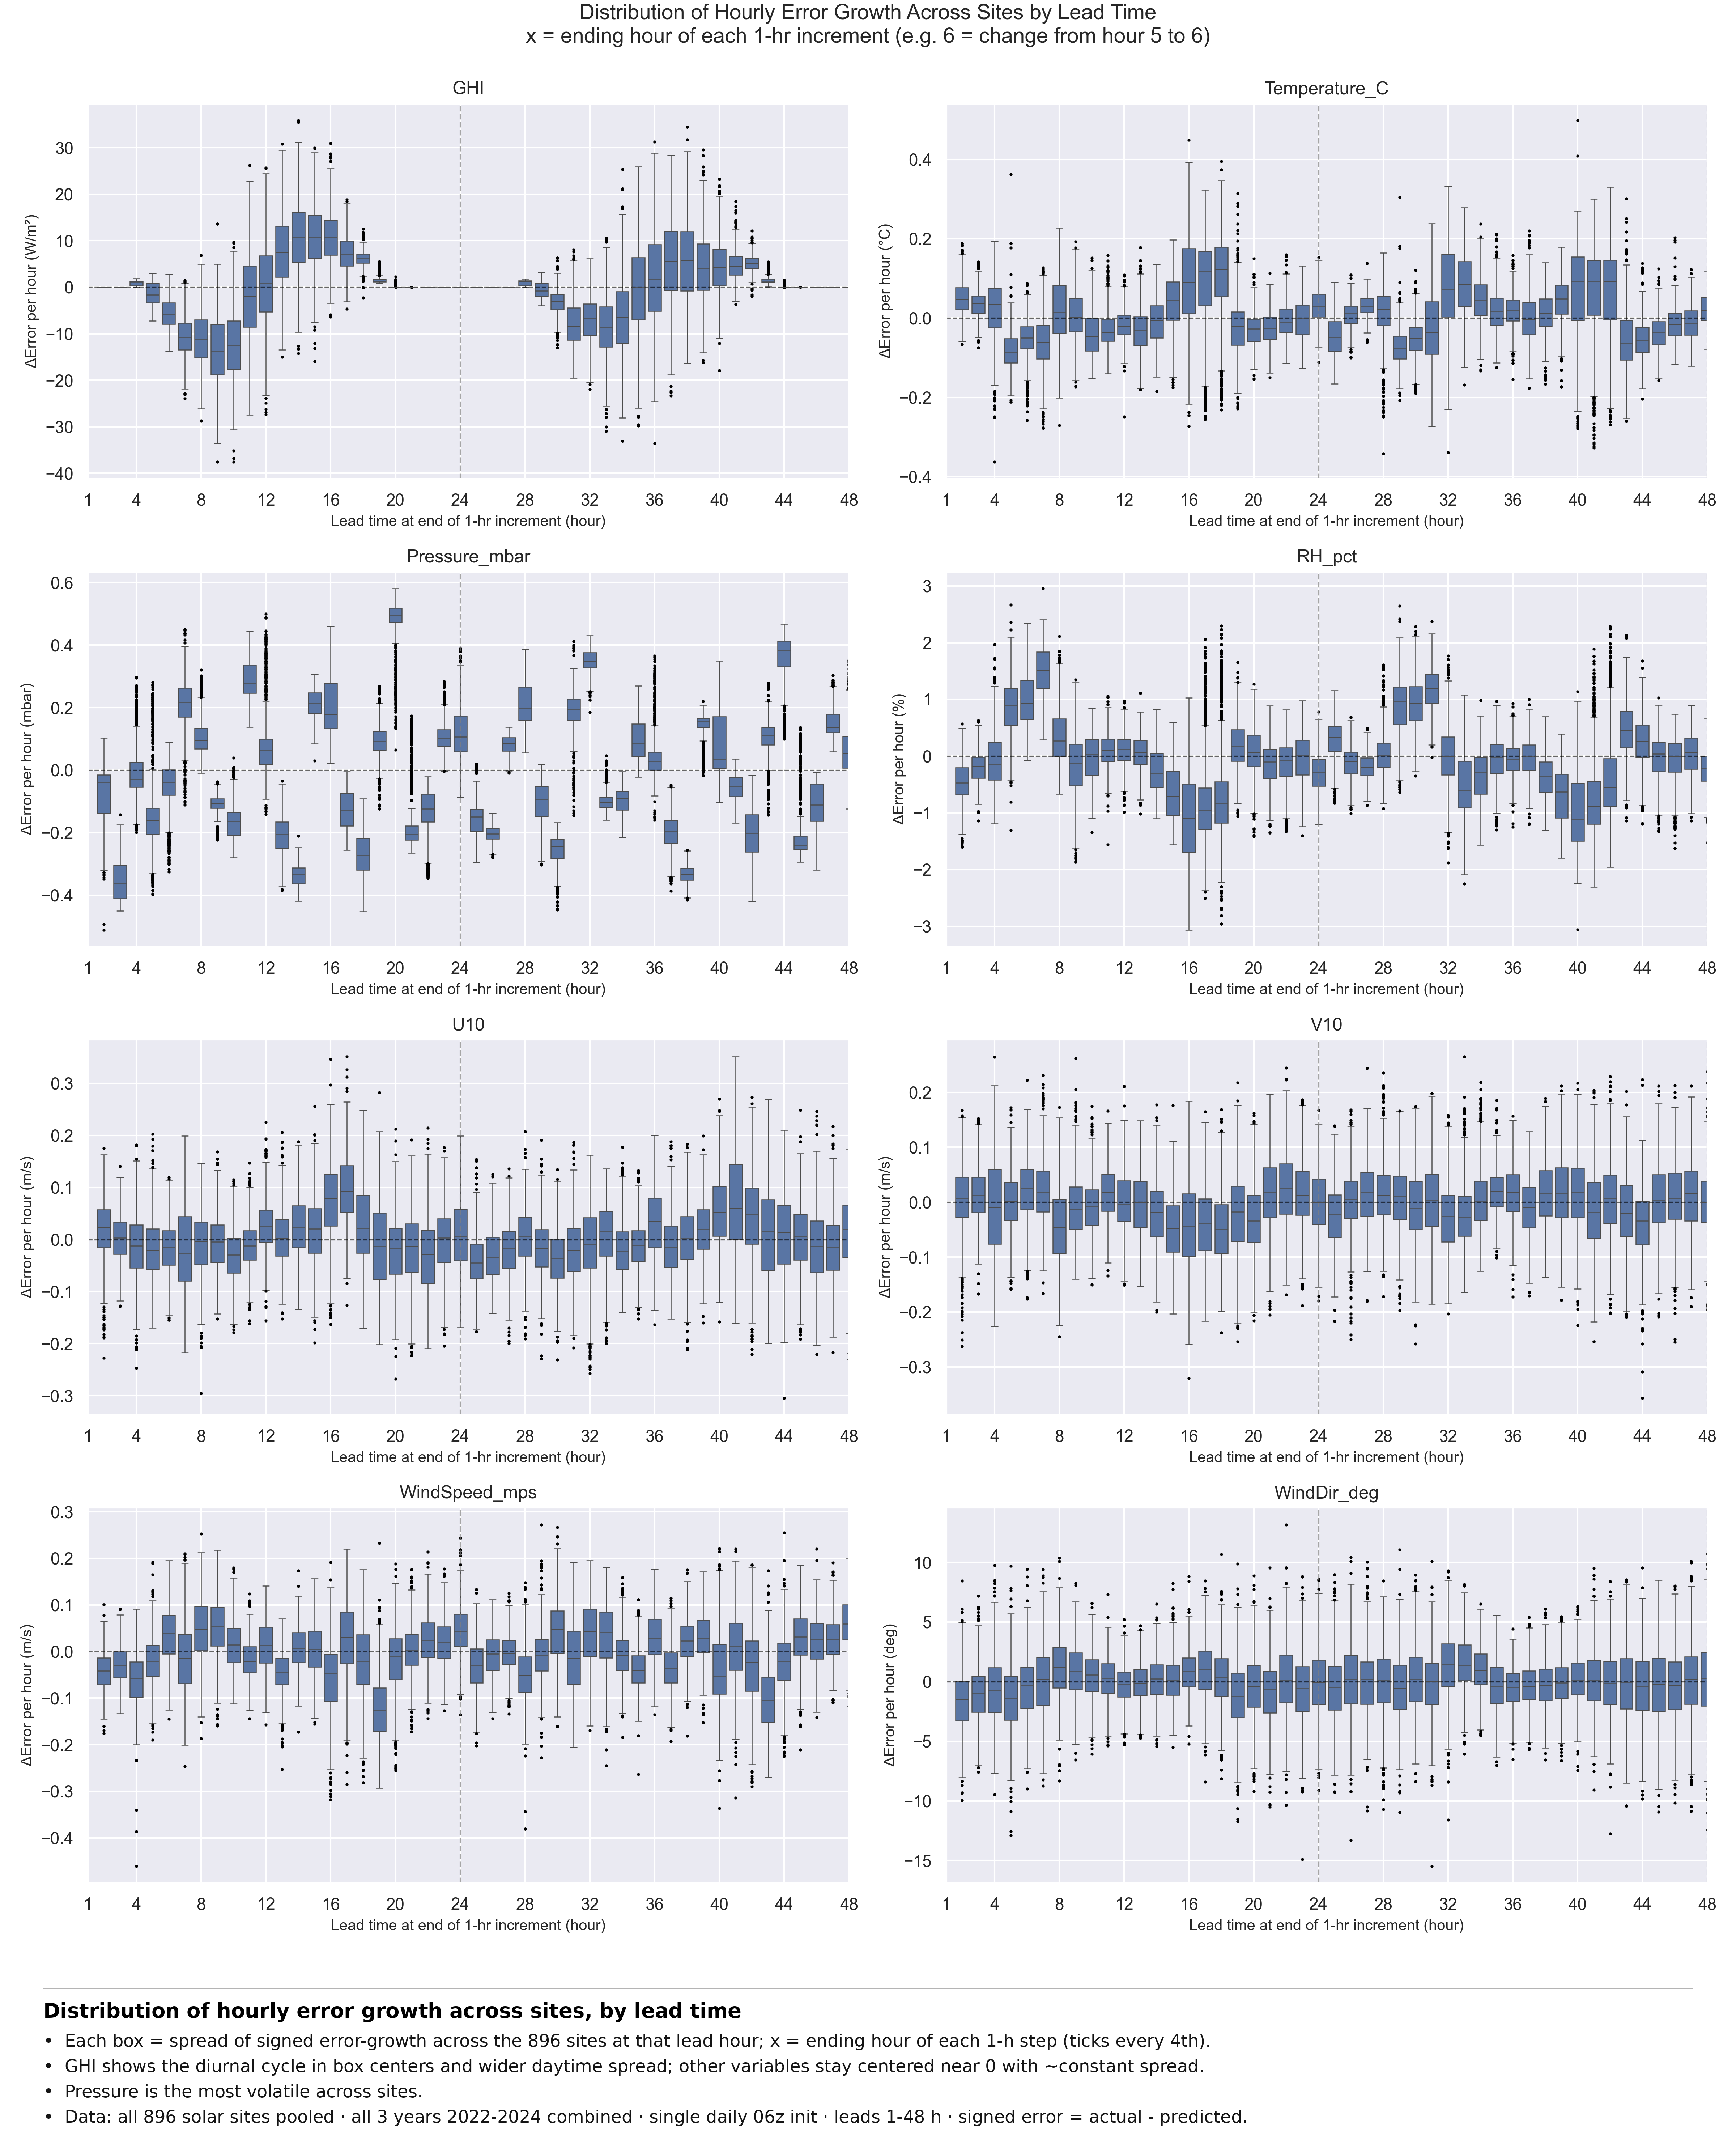
\includegraphics[width=\textwidth]{figures/Q2/error_growth_distributions.png}
  \caption{Complete (all-variable) version of the hourly error-growth distributions across sites.}
  \label{fig:app_growthdist}
\end{figure}

\begin{figure}[H]
  \centering
  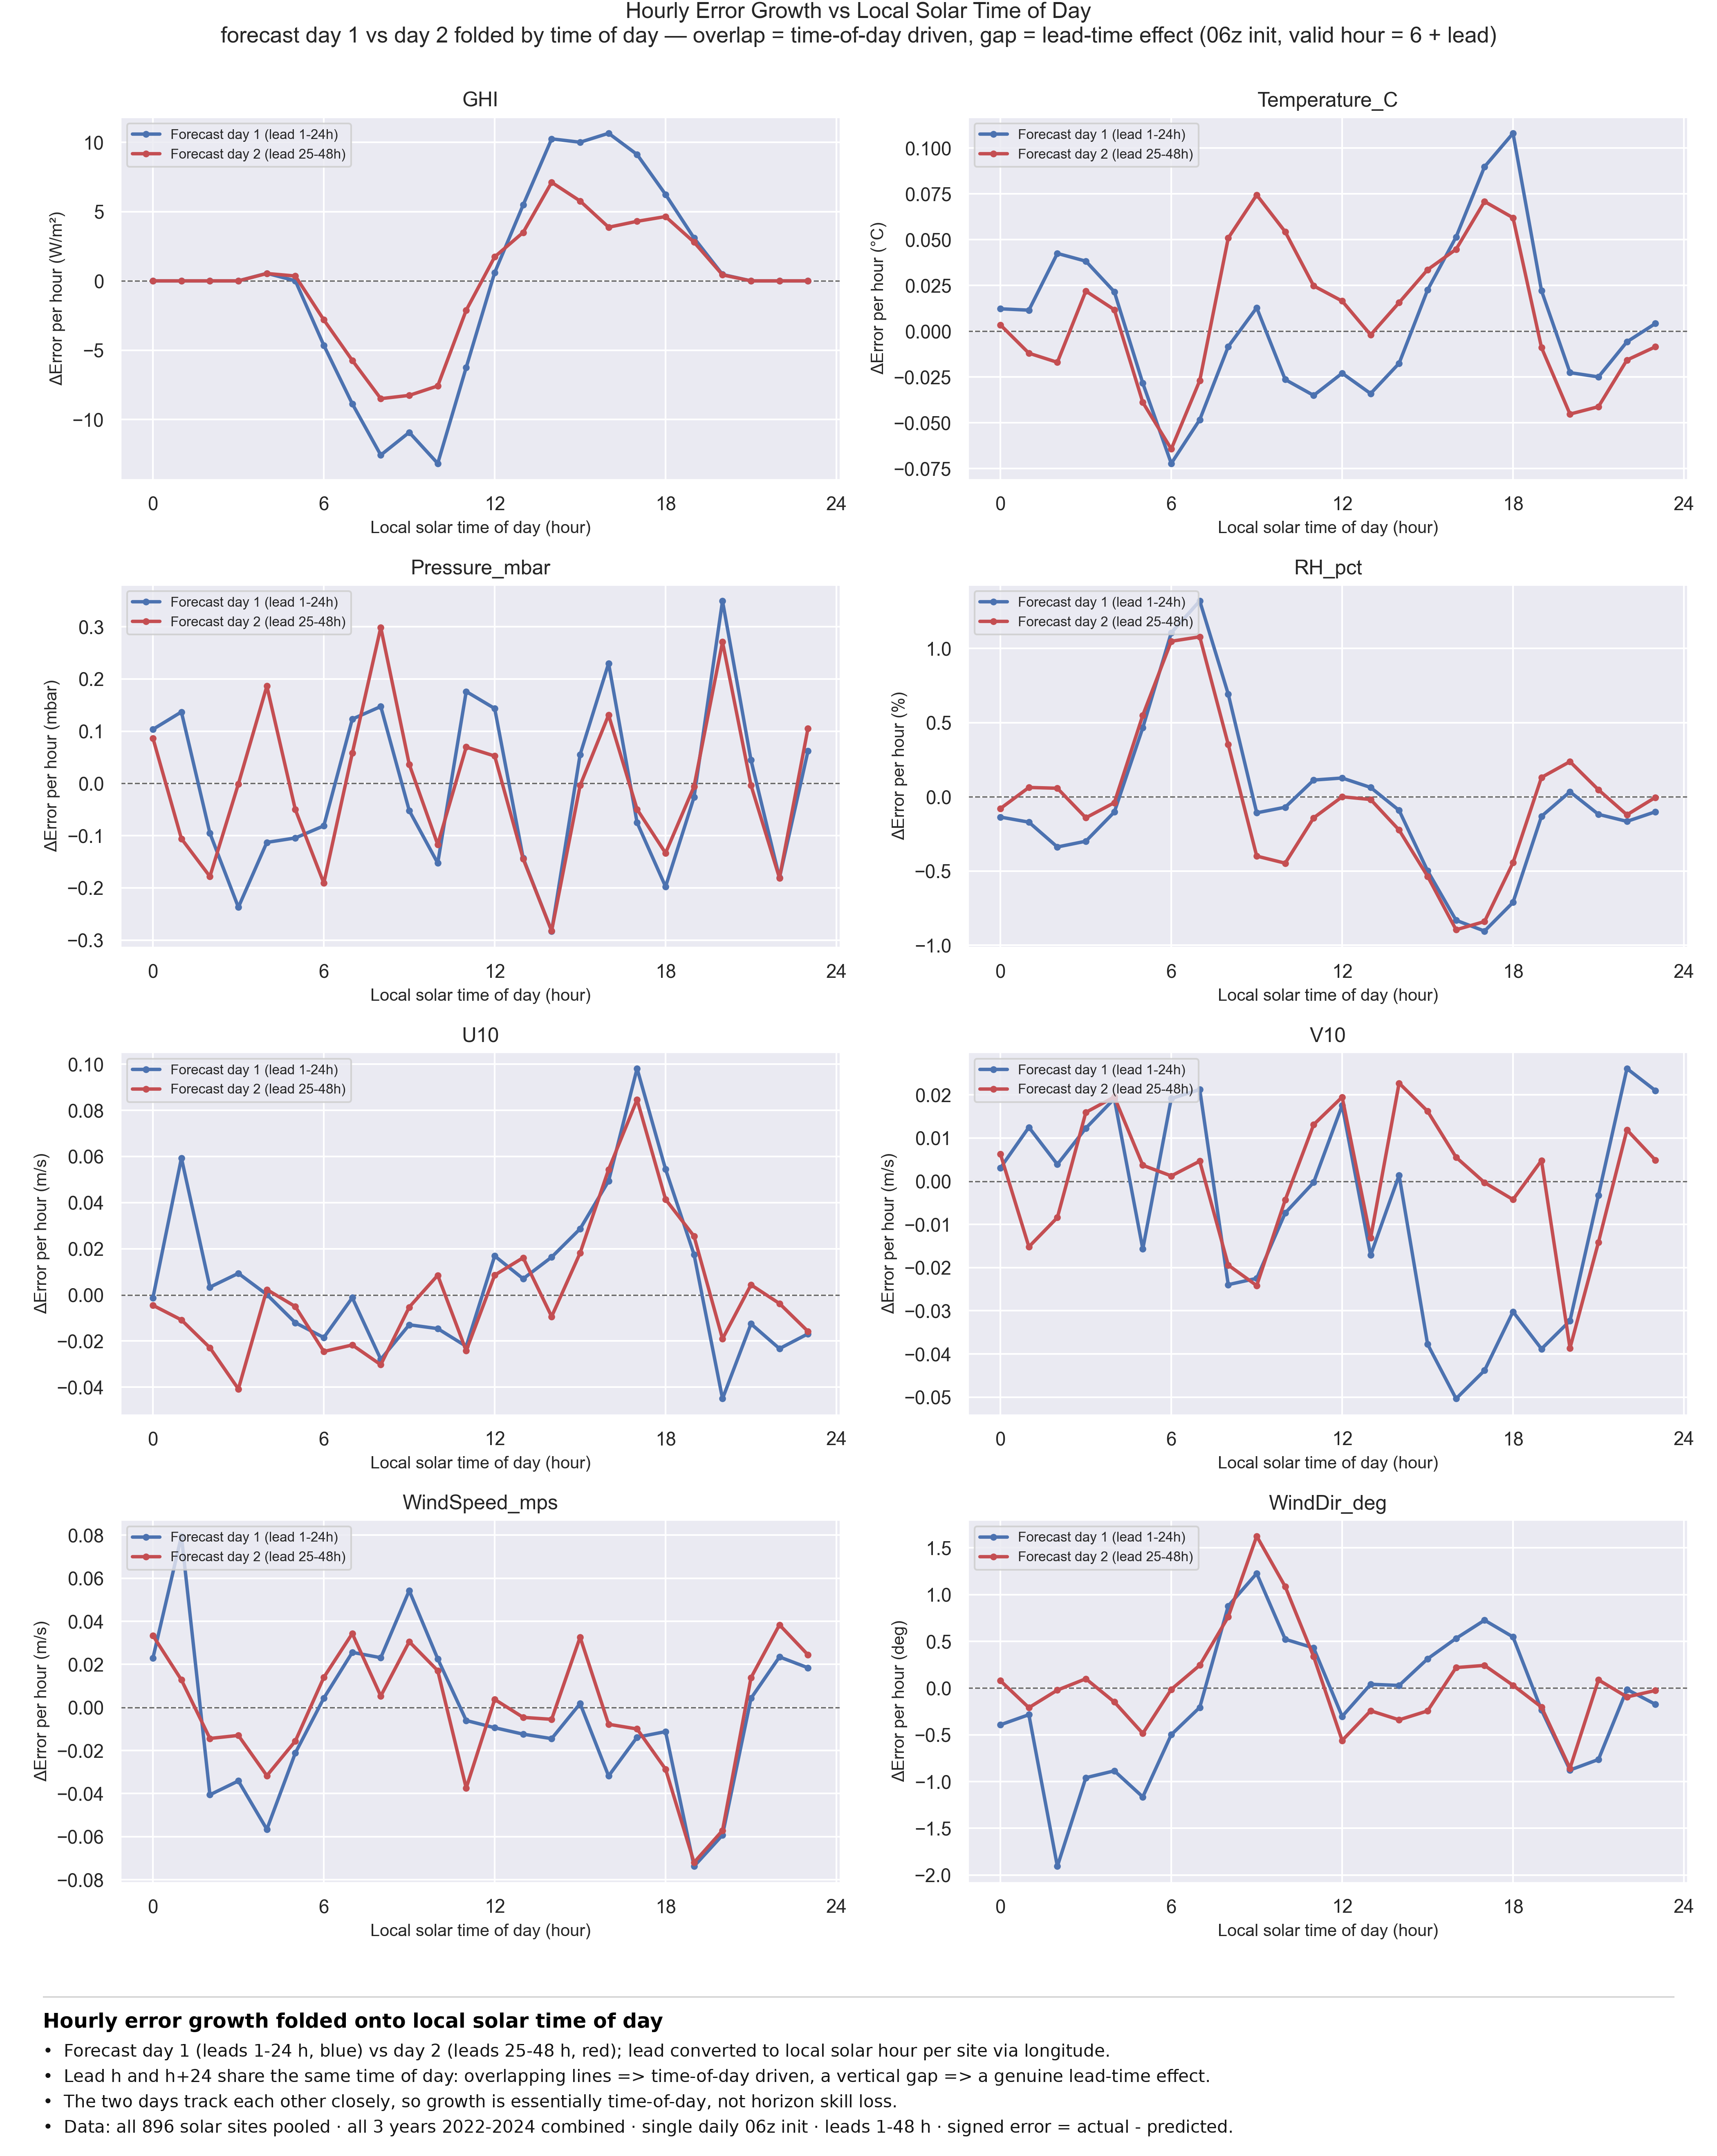
\includegraphics[width=\textwidth]{figures/Q2/error_growth_vs_time_of_day.png}
  \caption{Complete (all-variable) version of hourly error growth folded onto local solar time of day.}
  \label{fig:app_tod}
\end{figure}

\subsection{Q4 and Q5}

\begin{figure}[H]
    \centering
    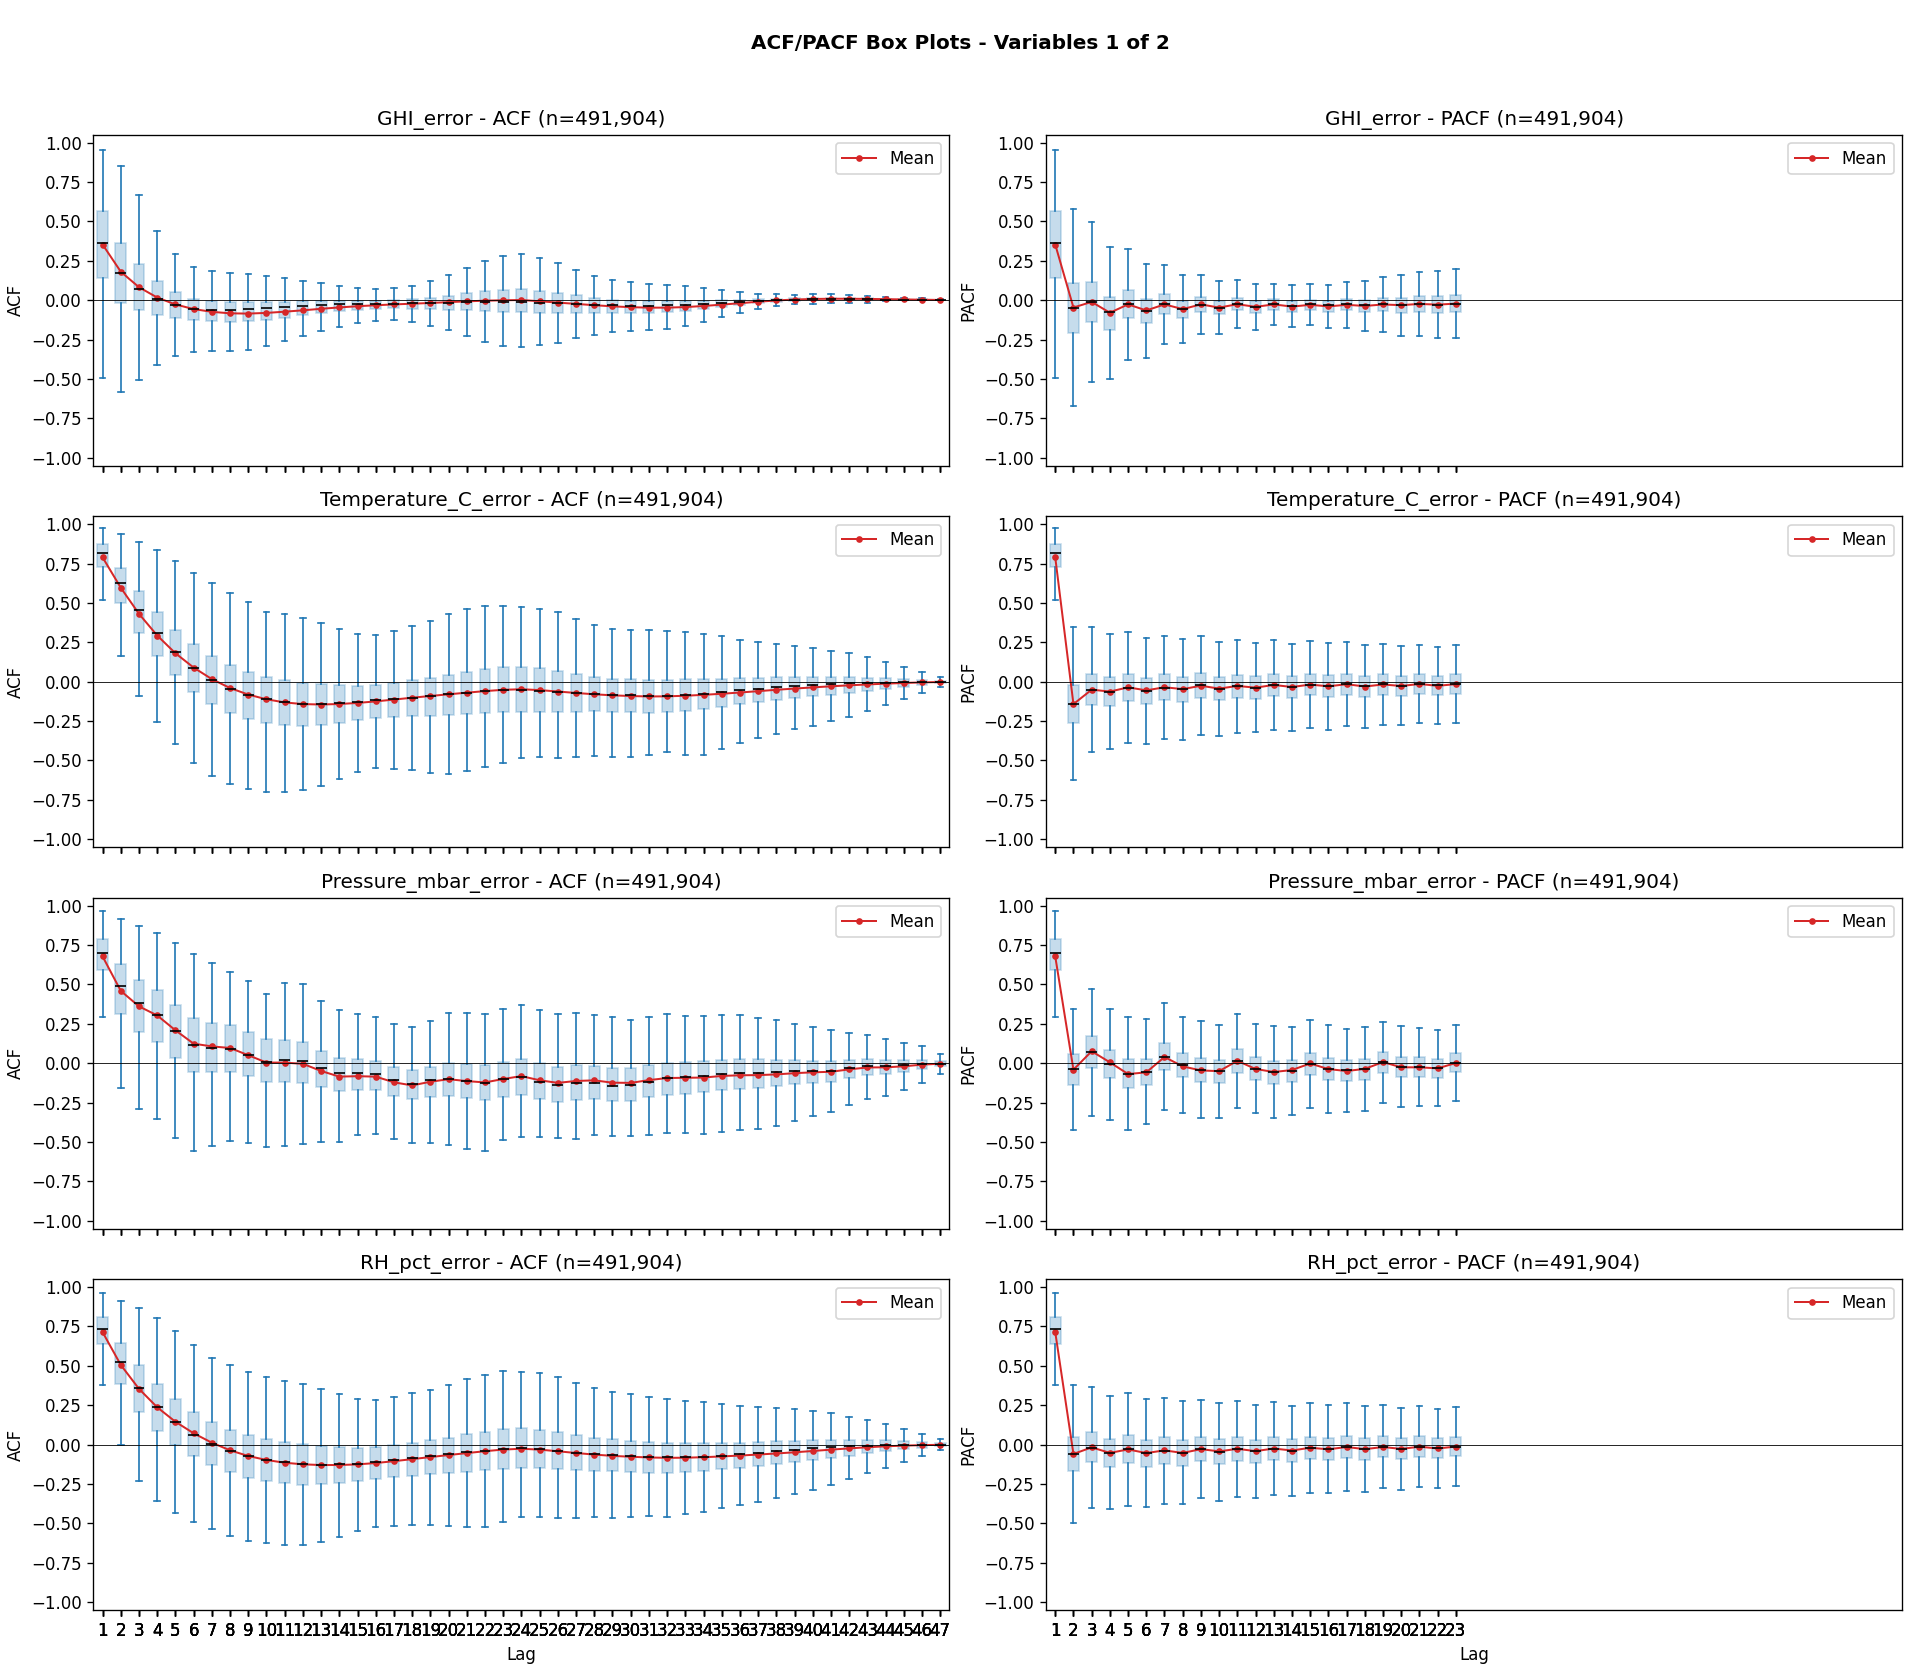
\includegraphics[width=\textwidth]{figures/Q4 & Q5/avg_acf_pacf_variables_01.png}
    \caption{ACF vs. lag on the left and PACF vs. lag on the right for GHI, temperature, pressure, and RH.}
    \label{fig:acf_pacf_vars1}
\end{figure}

\begin{figure}[H]
    \centering
    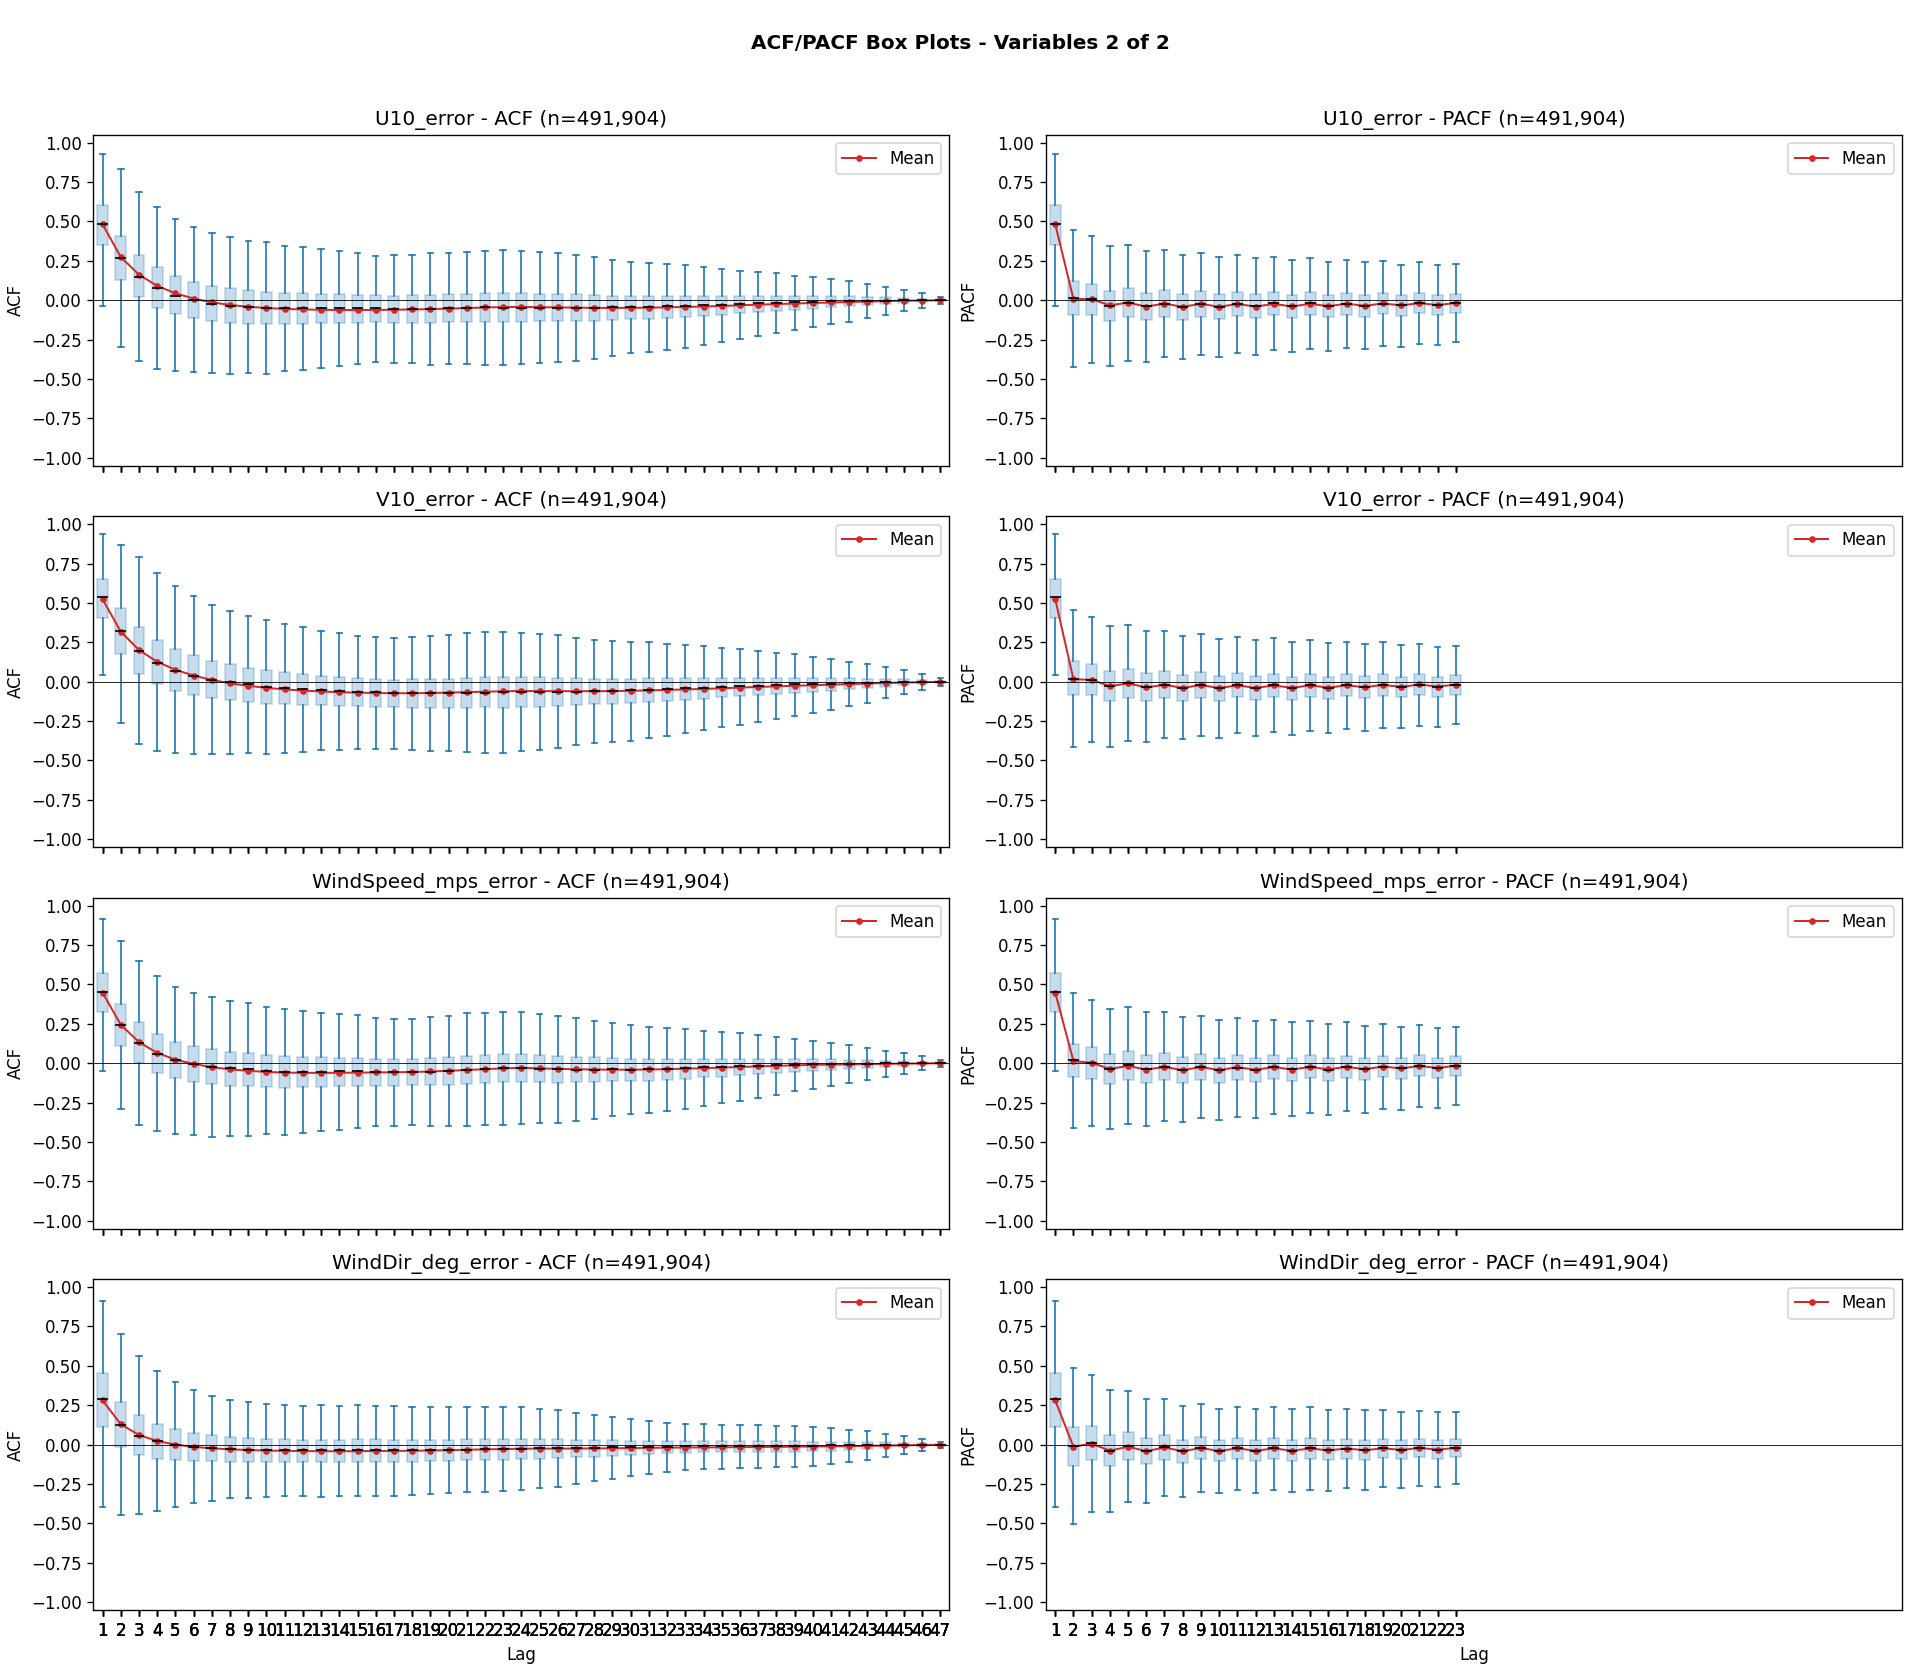
\includegraphics[width=\textwidth]{figures/Q4 & Q5/avg_acf_pacf_variables_02.png}
    \caption{ACF vs. lag on the left and PACF vs. lag on the right for U10, V10, wind speed, and wind direction.}
    \label{fig:acf_pacf_vars2}
\end{figure}

\subsection{Q7 — Stratified Cross-Variable Error Matrices}

% --- DIURNAL EVOLUTION ---
\begin{figure}[H]
  \centering
  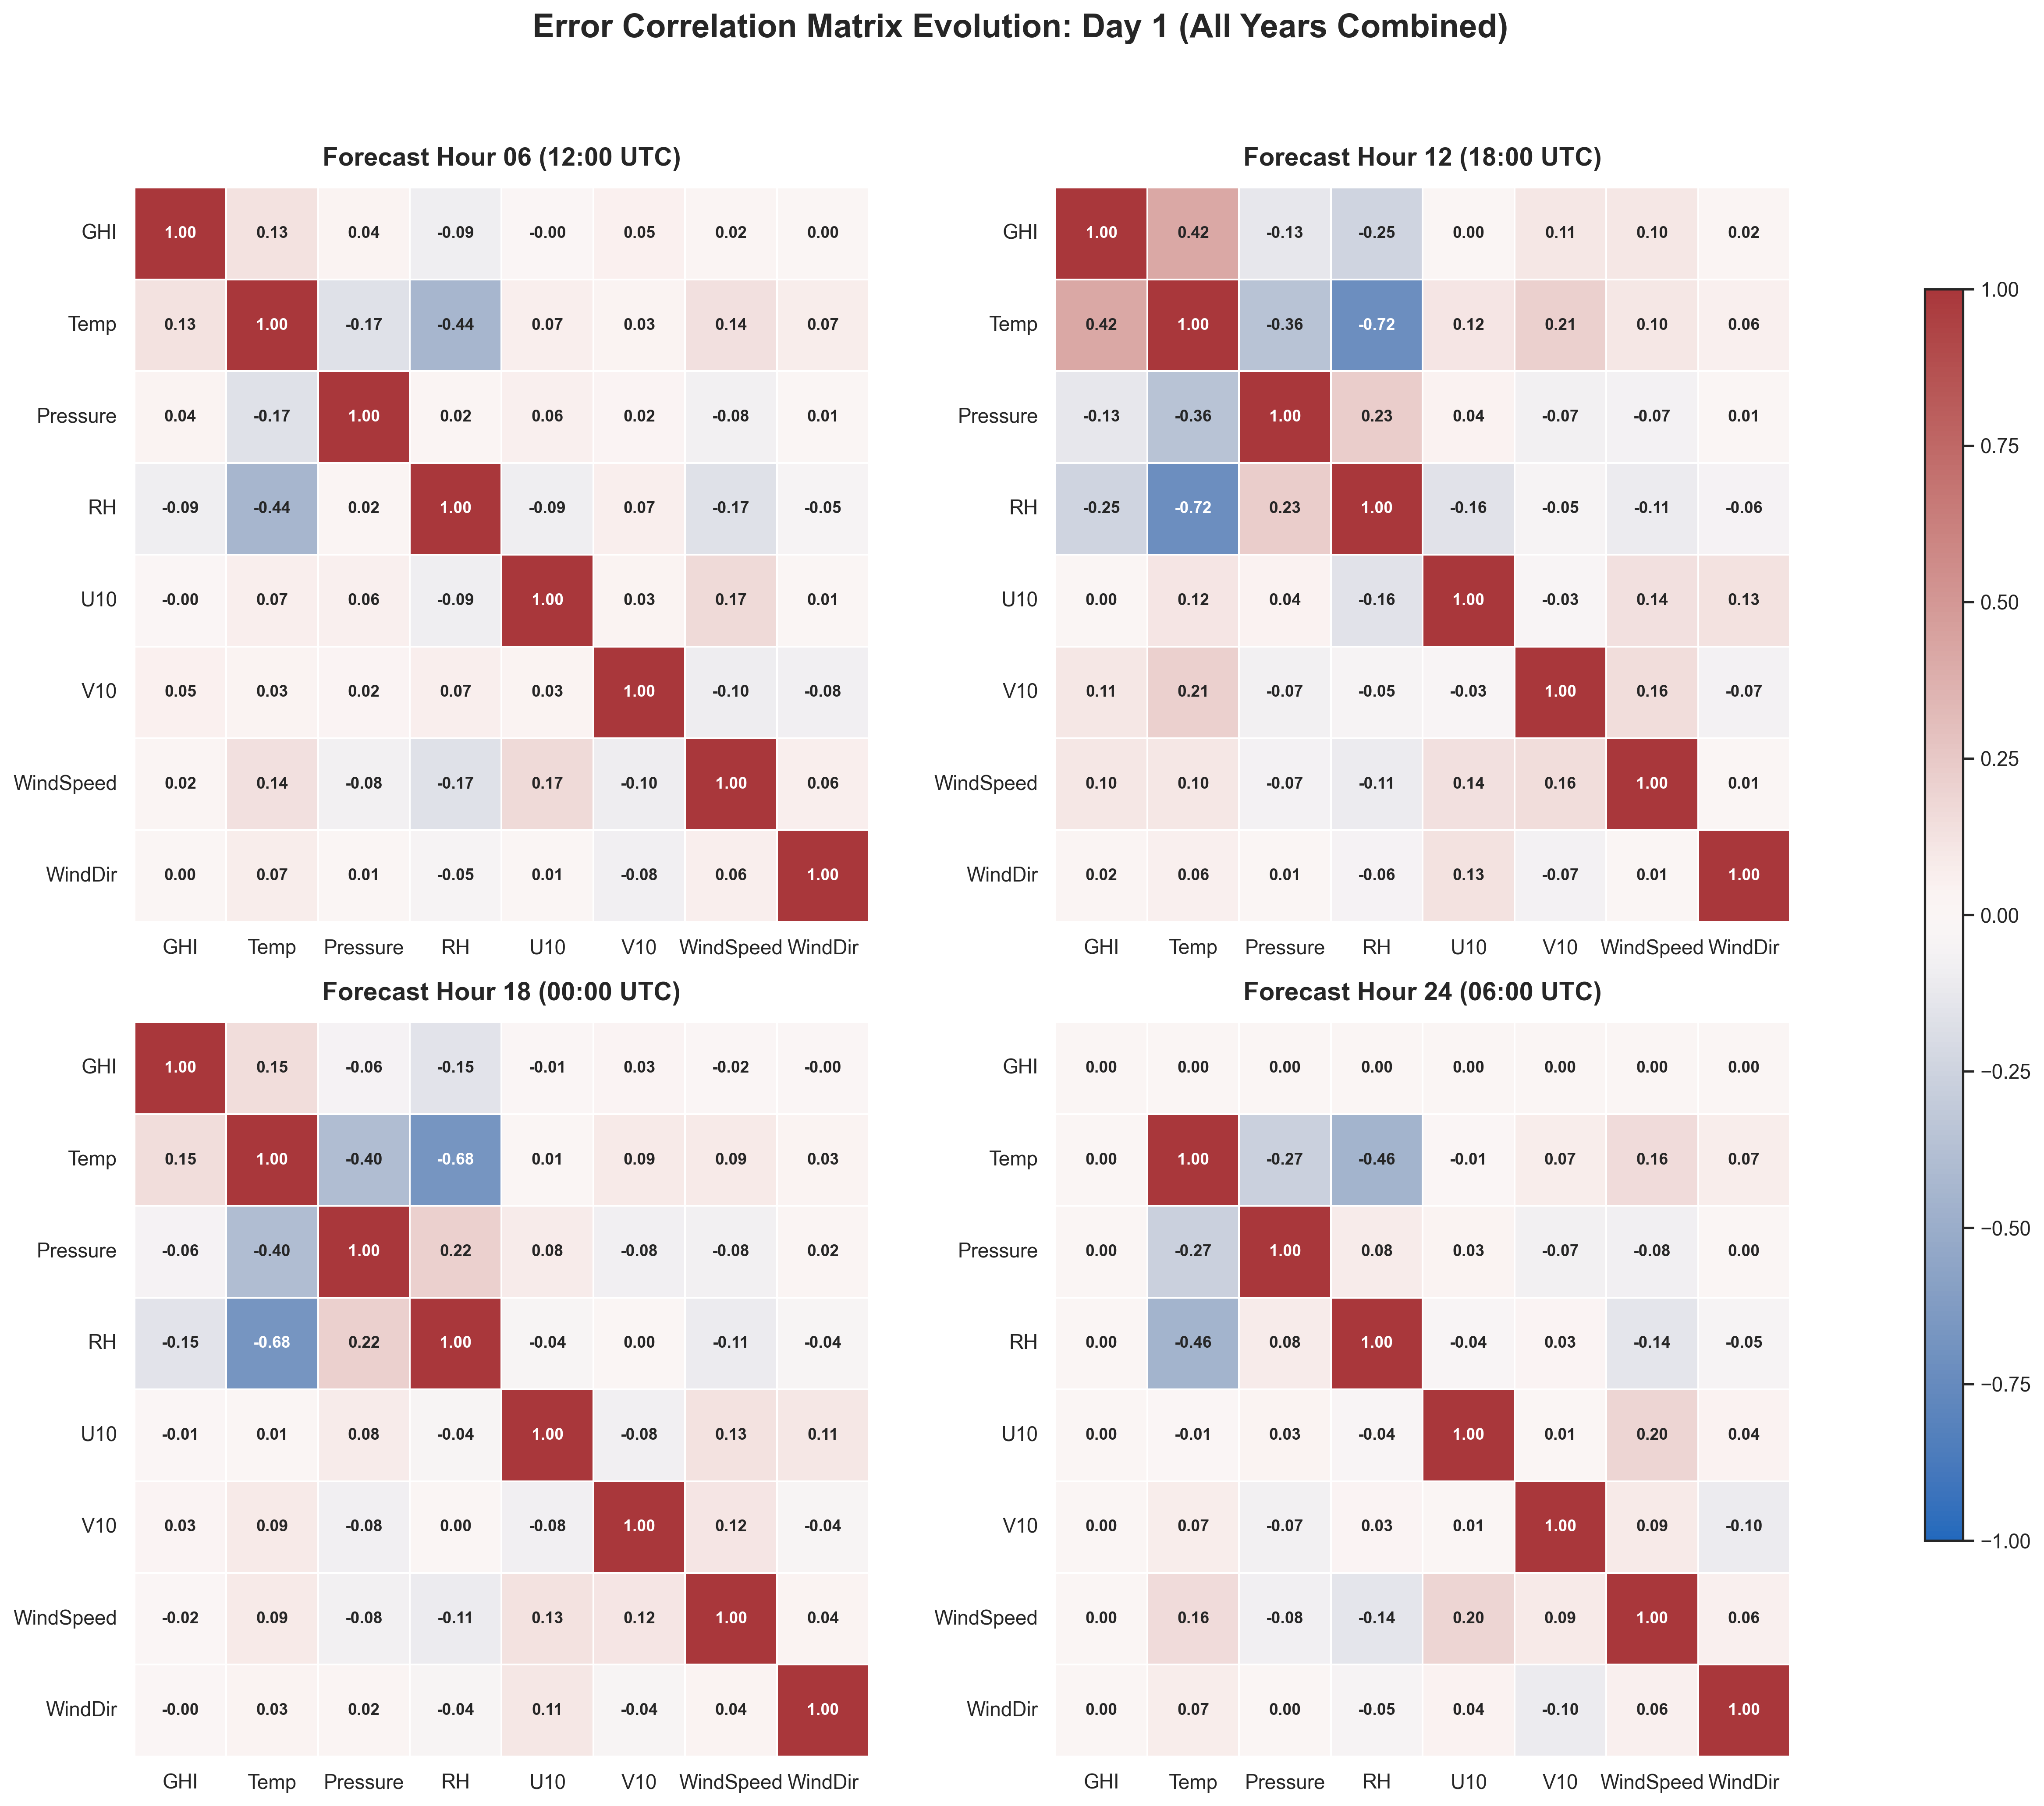
\includegraphics[width=\textwidth]{figures/Q7/TIMEOFDAY/all_variables_corr_day1_horizons.png}
  \caption{Error Correlation Matrix Evolution: Day 1 hourly snapshots across all years combined.}
  \label{fig:app_diurnal_evolution}
\end{figure}

% --- SEASONAL VARIATIONS ---
\begin{figure}[H]
  \centering
  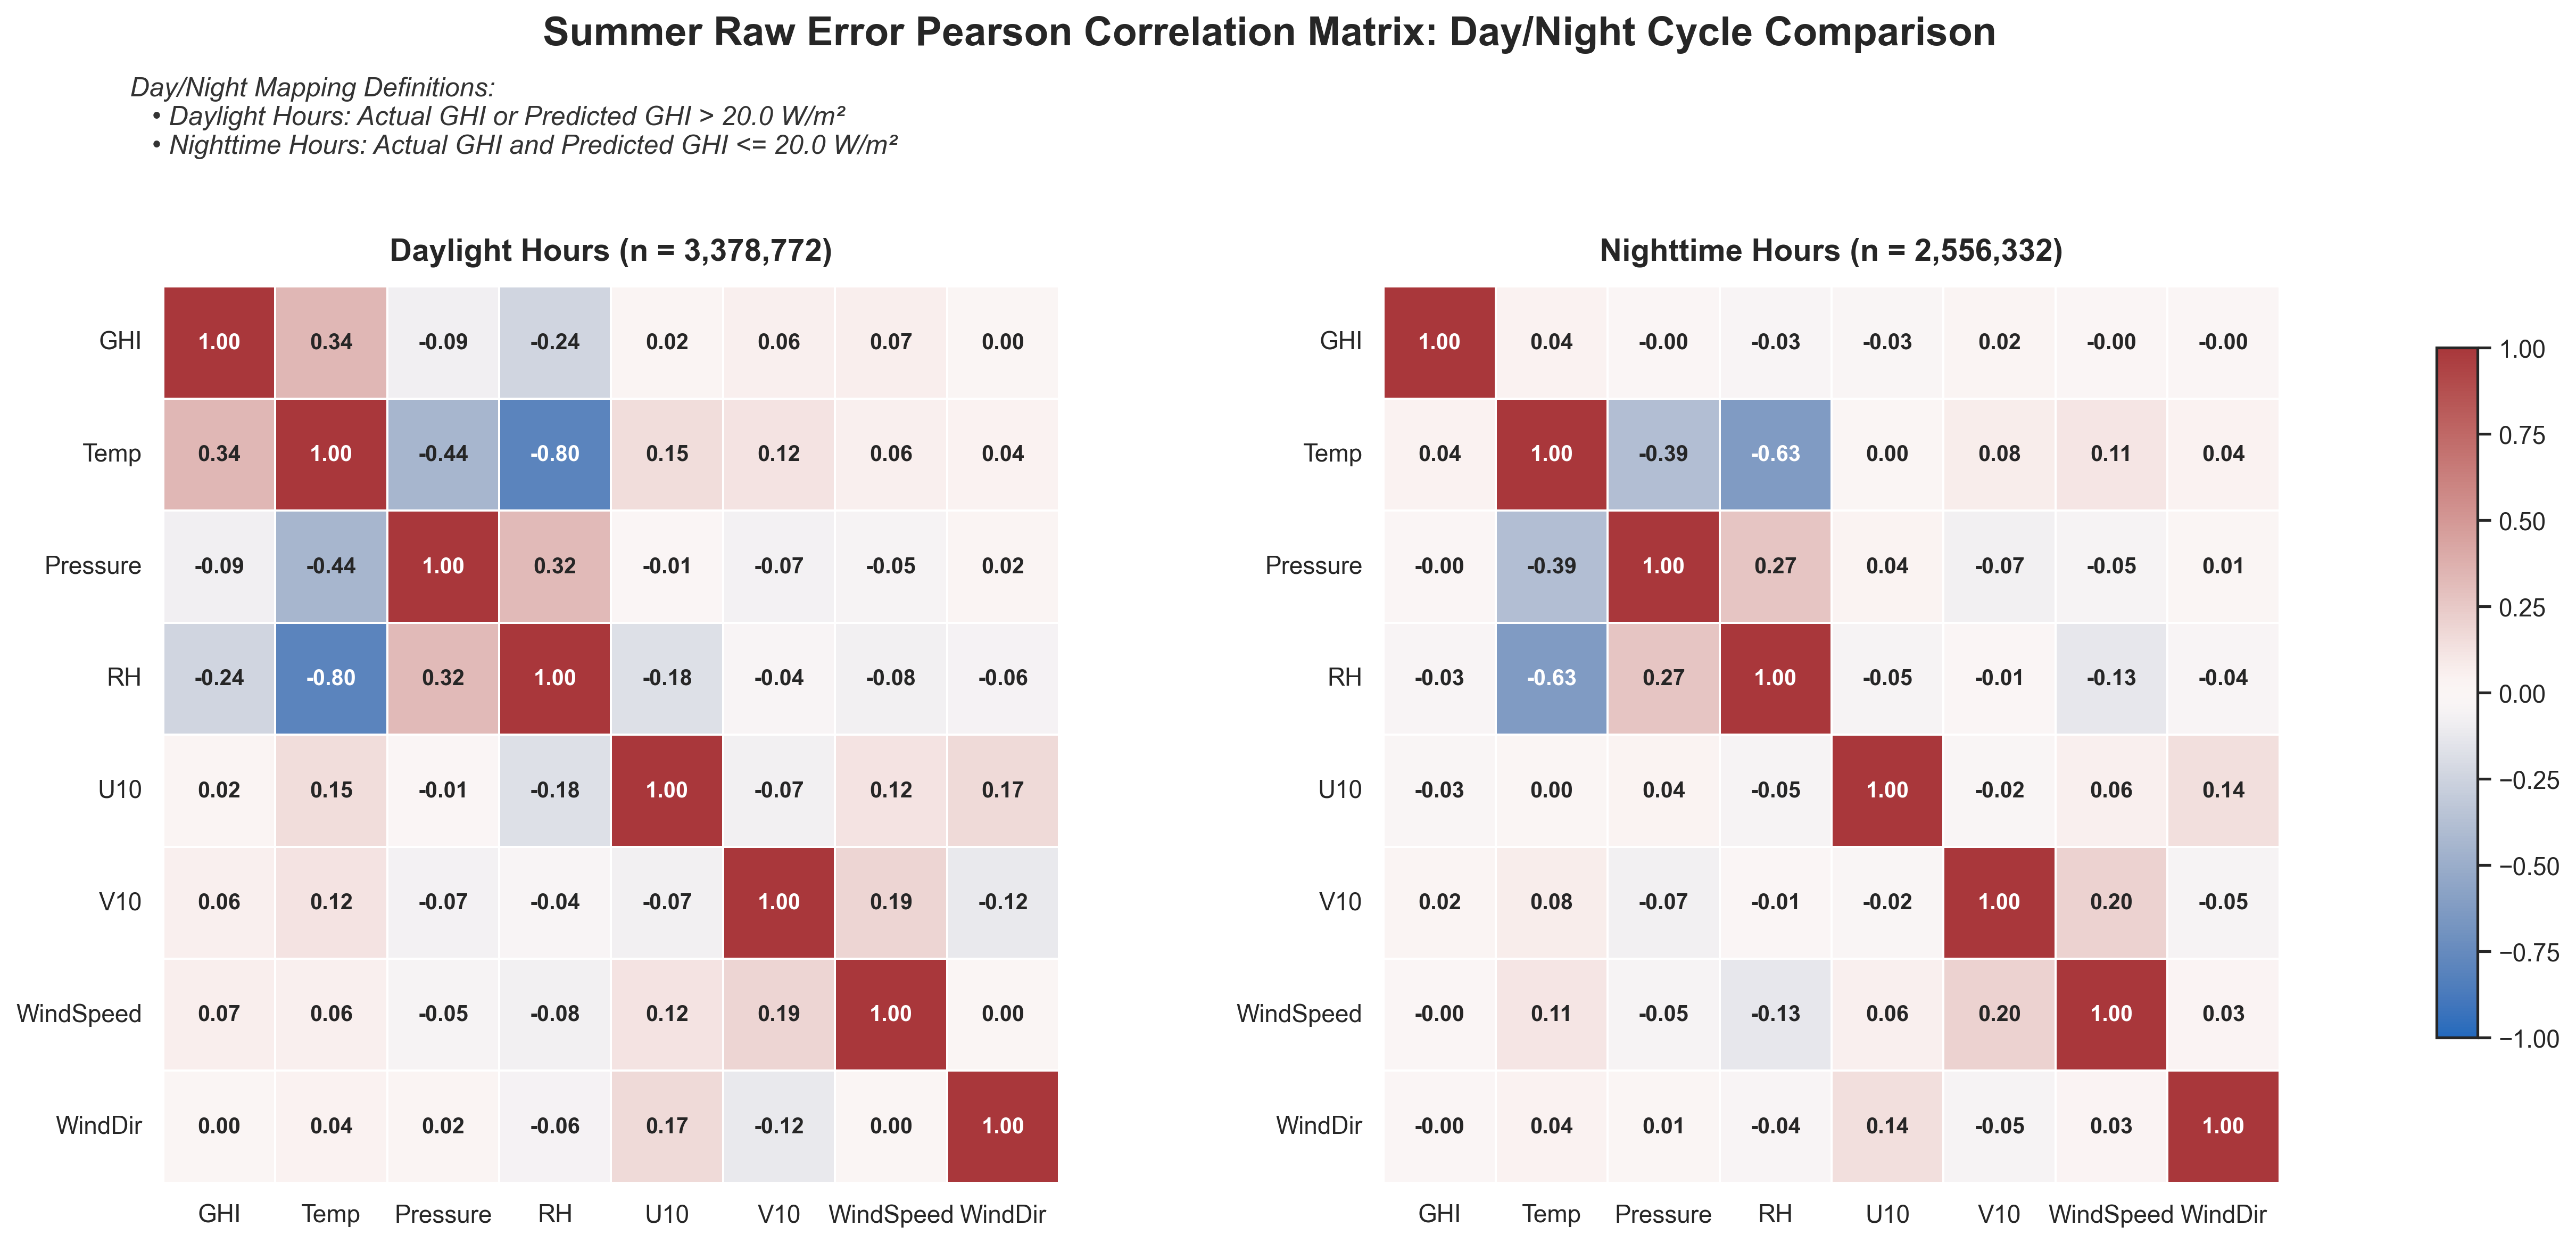
\includegraphics[width=\textwidth]{figures/Q7/SEASONS/correlation_heatmap_summer_diurnal_comparison.png}
  \caption{Summer Raw Error Pearson Correlation Matrix: Daylight Hours ($n = 3,378,772$, left) versus Nighttime Hours ($n = 2,556,332$, right) comparison.}
  \label{fig:app_summer_day_night}
\end{figure}

\begin{figure}[H]
  \centering
  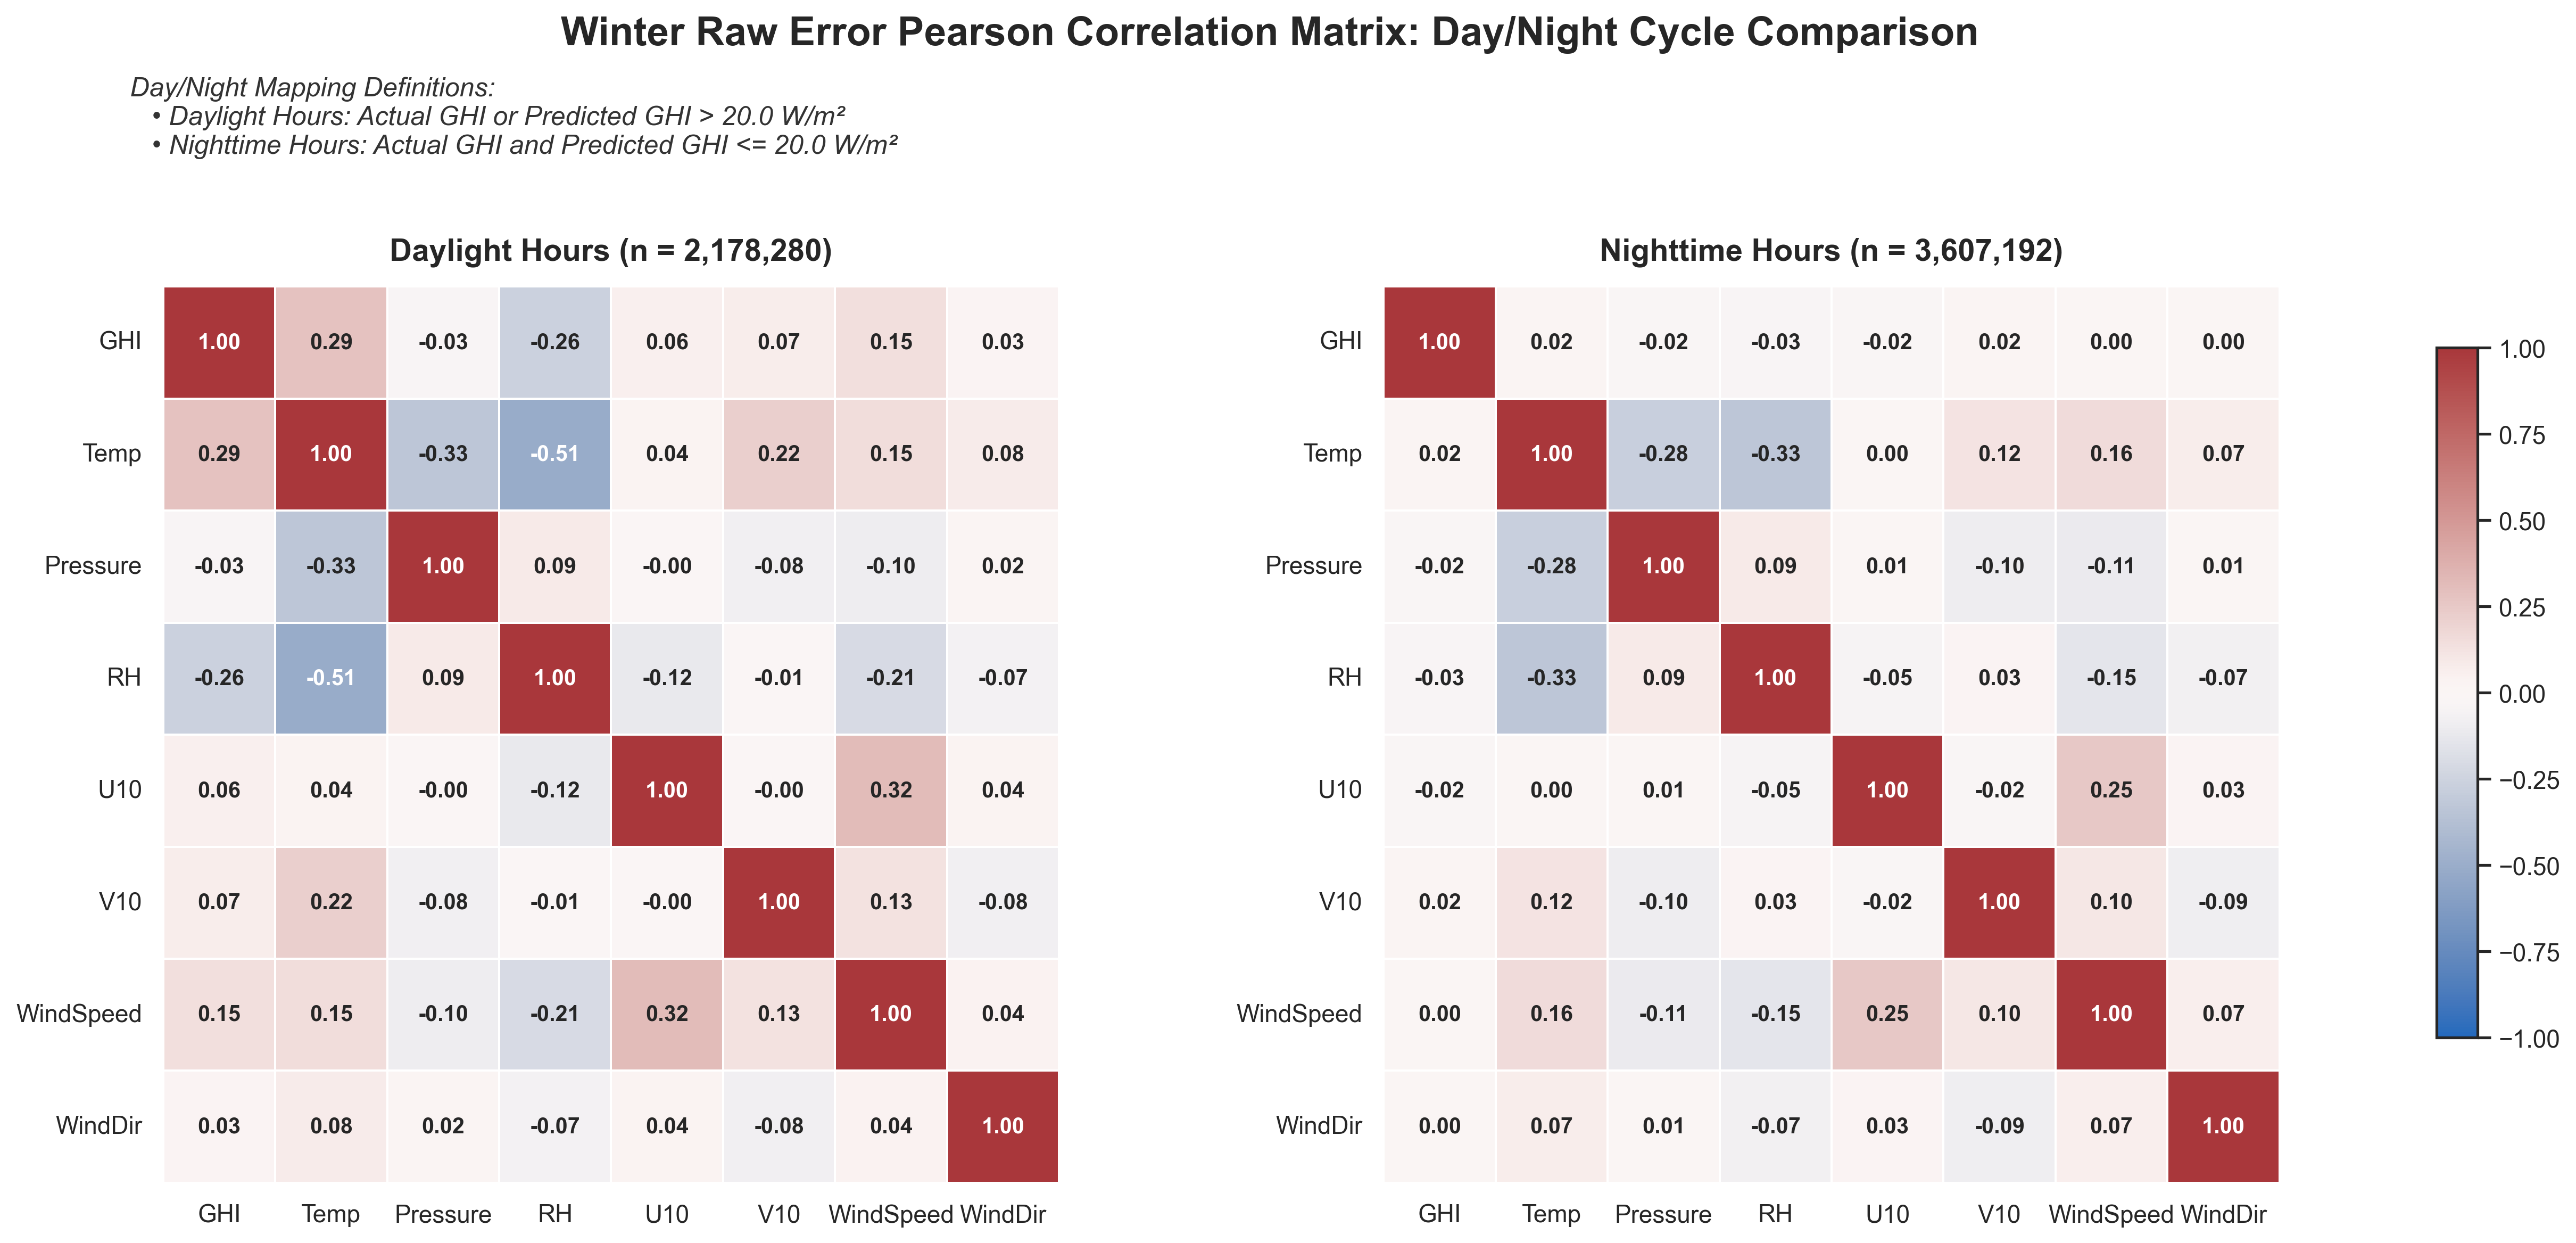
\includegraphics[width=\textwidth]{figures/Q7/SEASONS/correlation_heatmap_winter_diurnal_comparison.png}
  \caption{Winter Raw Error Pearson Correlation Matrix: Daylight vs. Nighttime comparison.}
  \label{fig:app_winter_day_night}
\end{figure}

\begin{figure}[H]
  \centering
  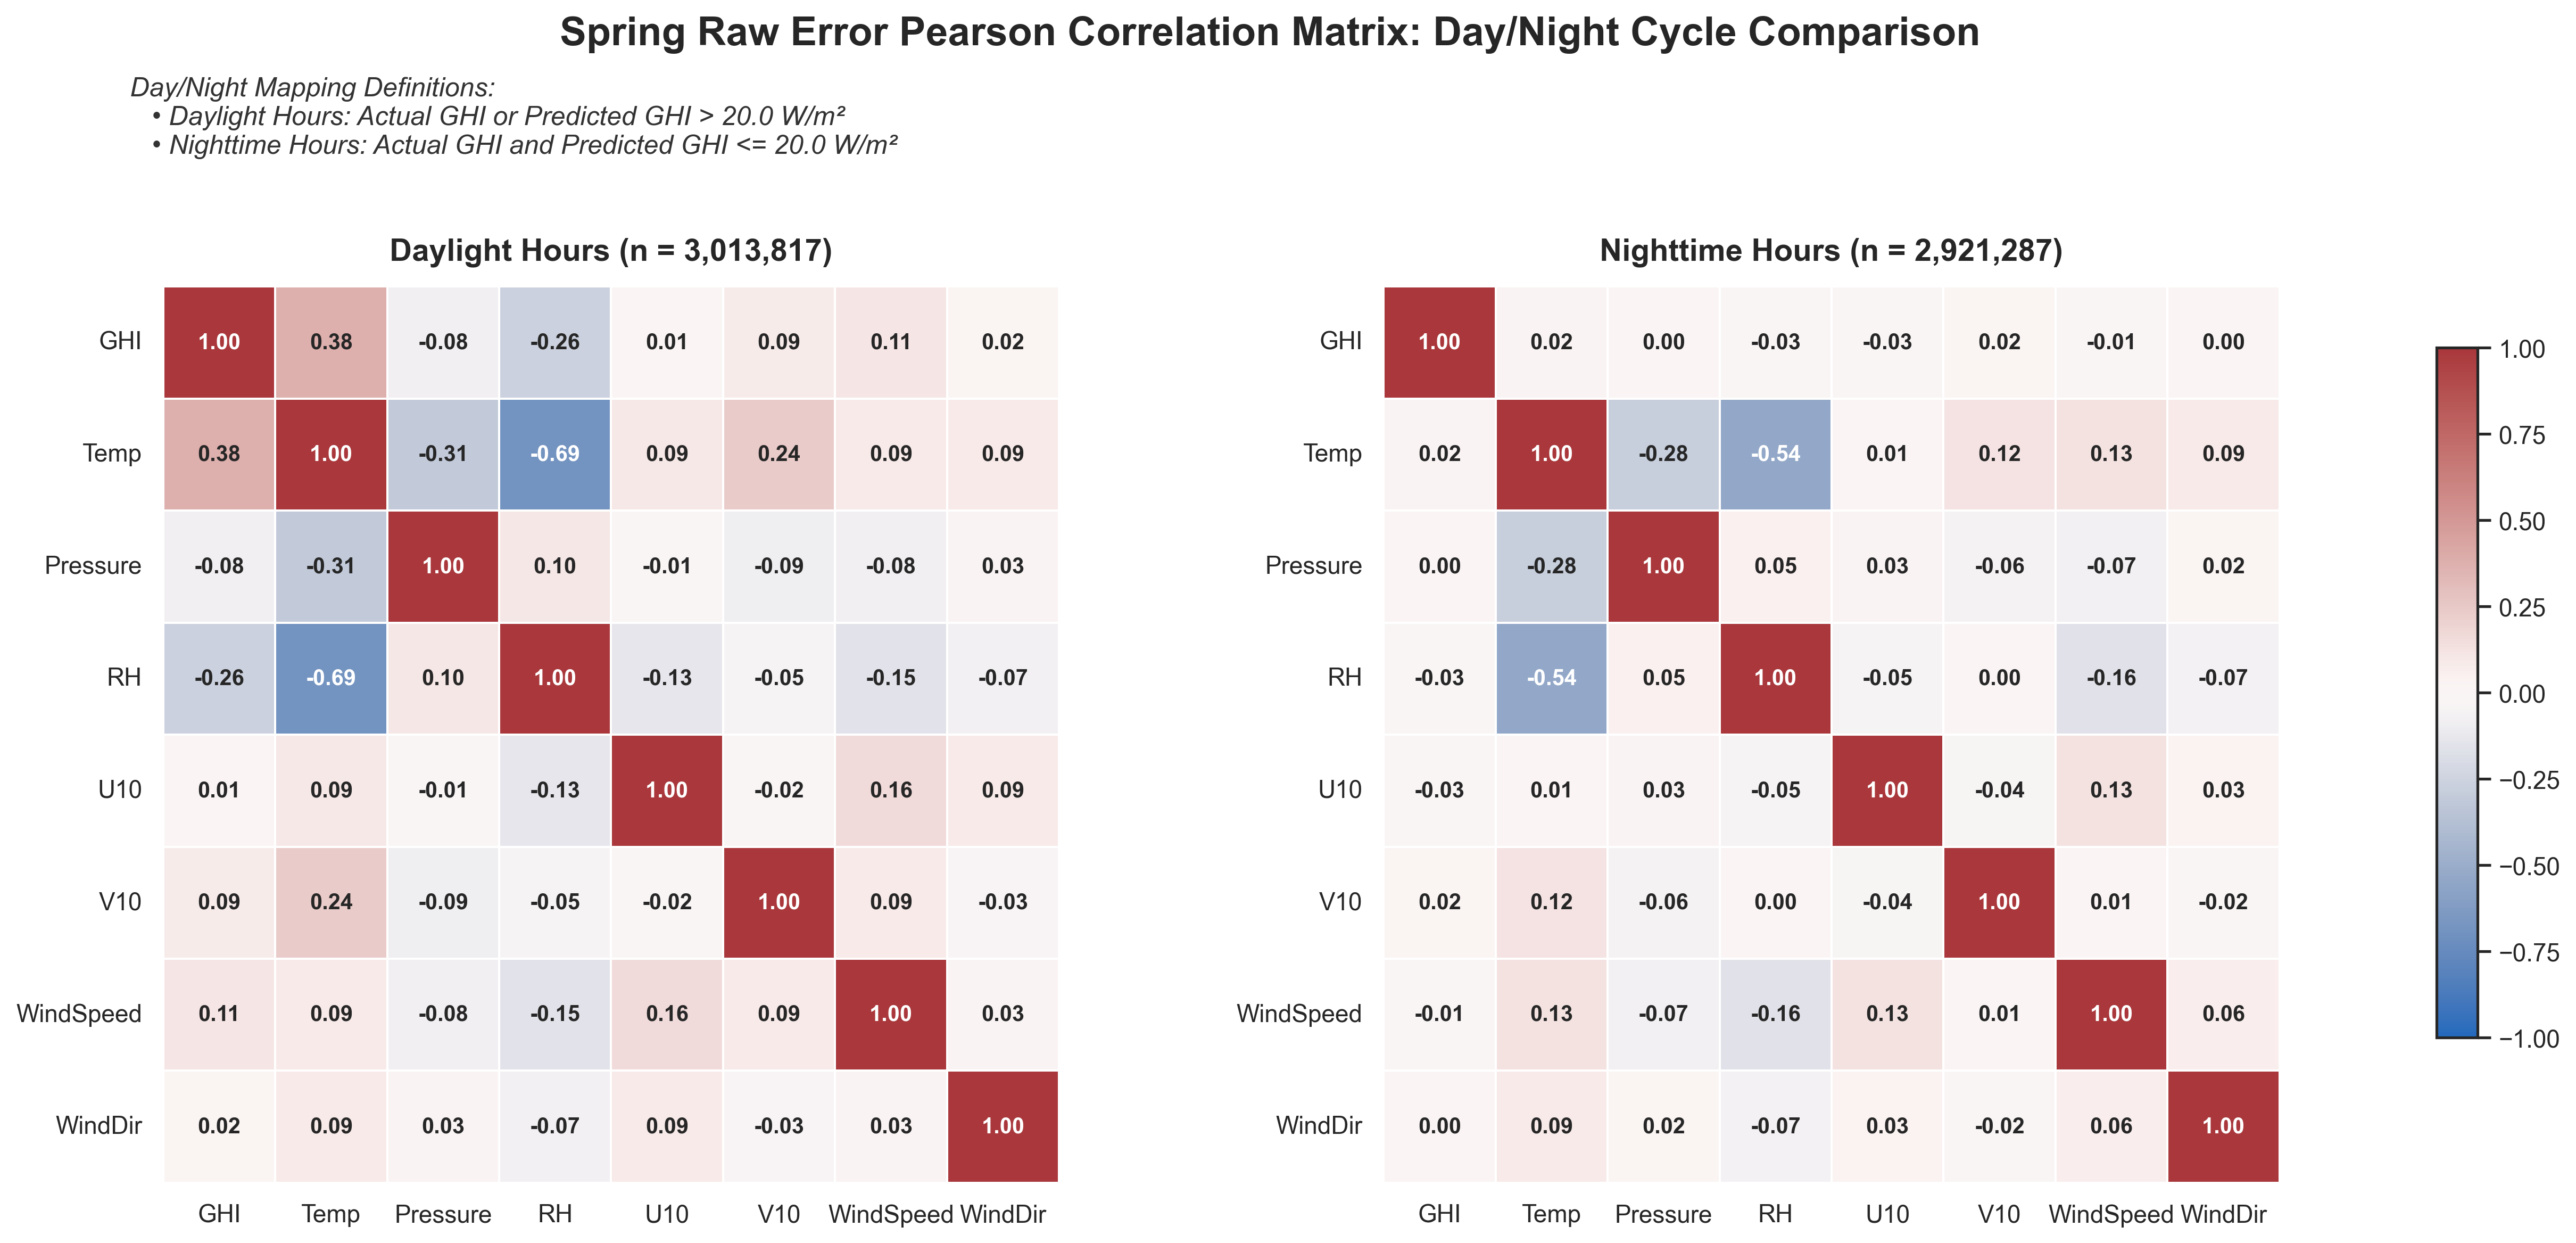
\includegraphics[width=\textwidth]{figures/Q7/SEASONS/correlation_heatmap_spring_diurnal_comparison.png}
  \caption{Spring Raw Error Pearson Correlation Matrix: Daylight Hours ($n = 3,013,817$, left) versus Nighttime Hours ($n = 2,921,287$, right) comparison.}
  \label{fig:app_spring_day_night}
\end{figure}

\begin{figure}[H]
  \centering
  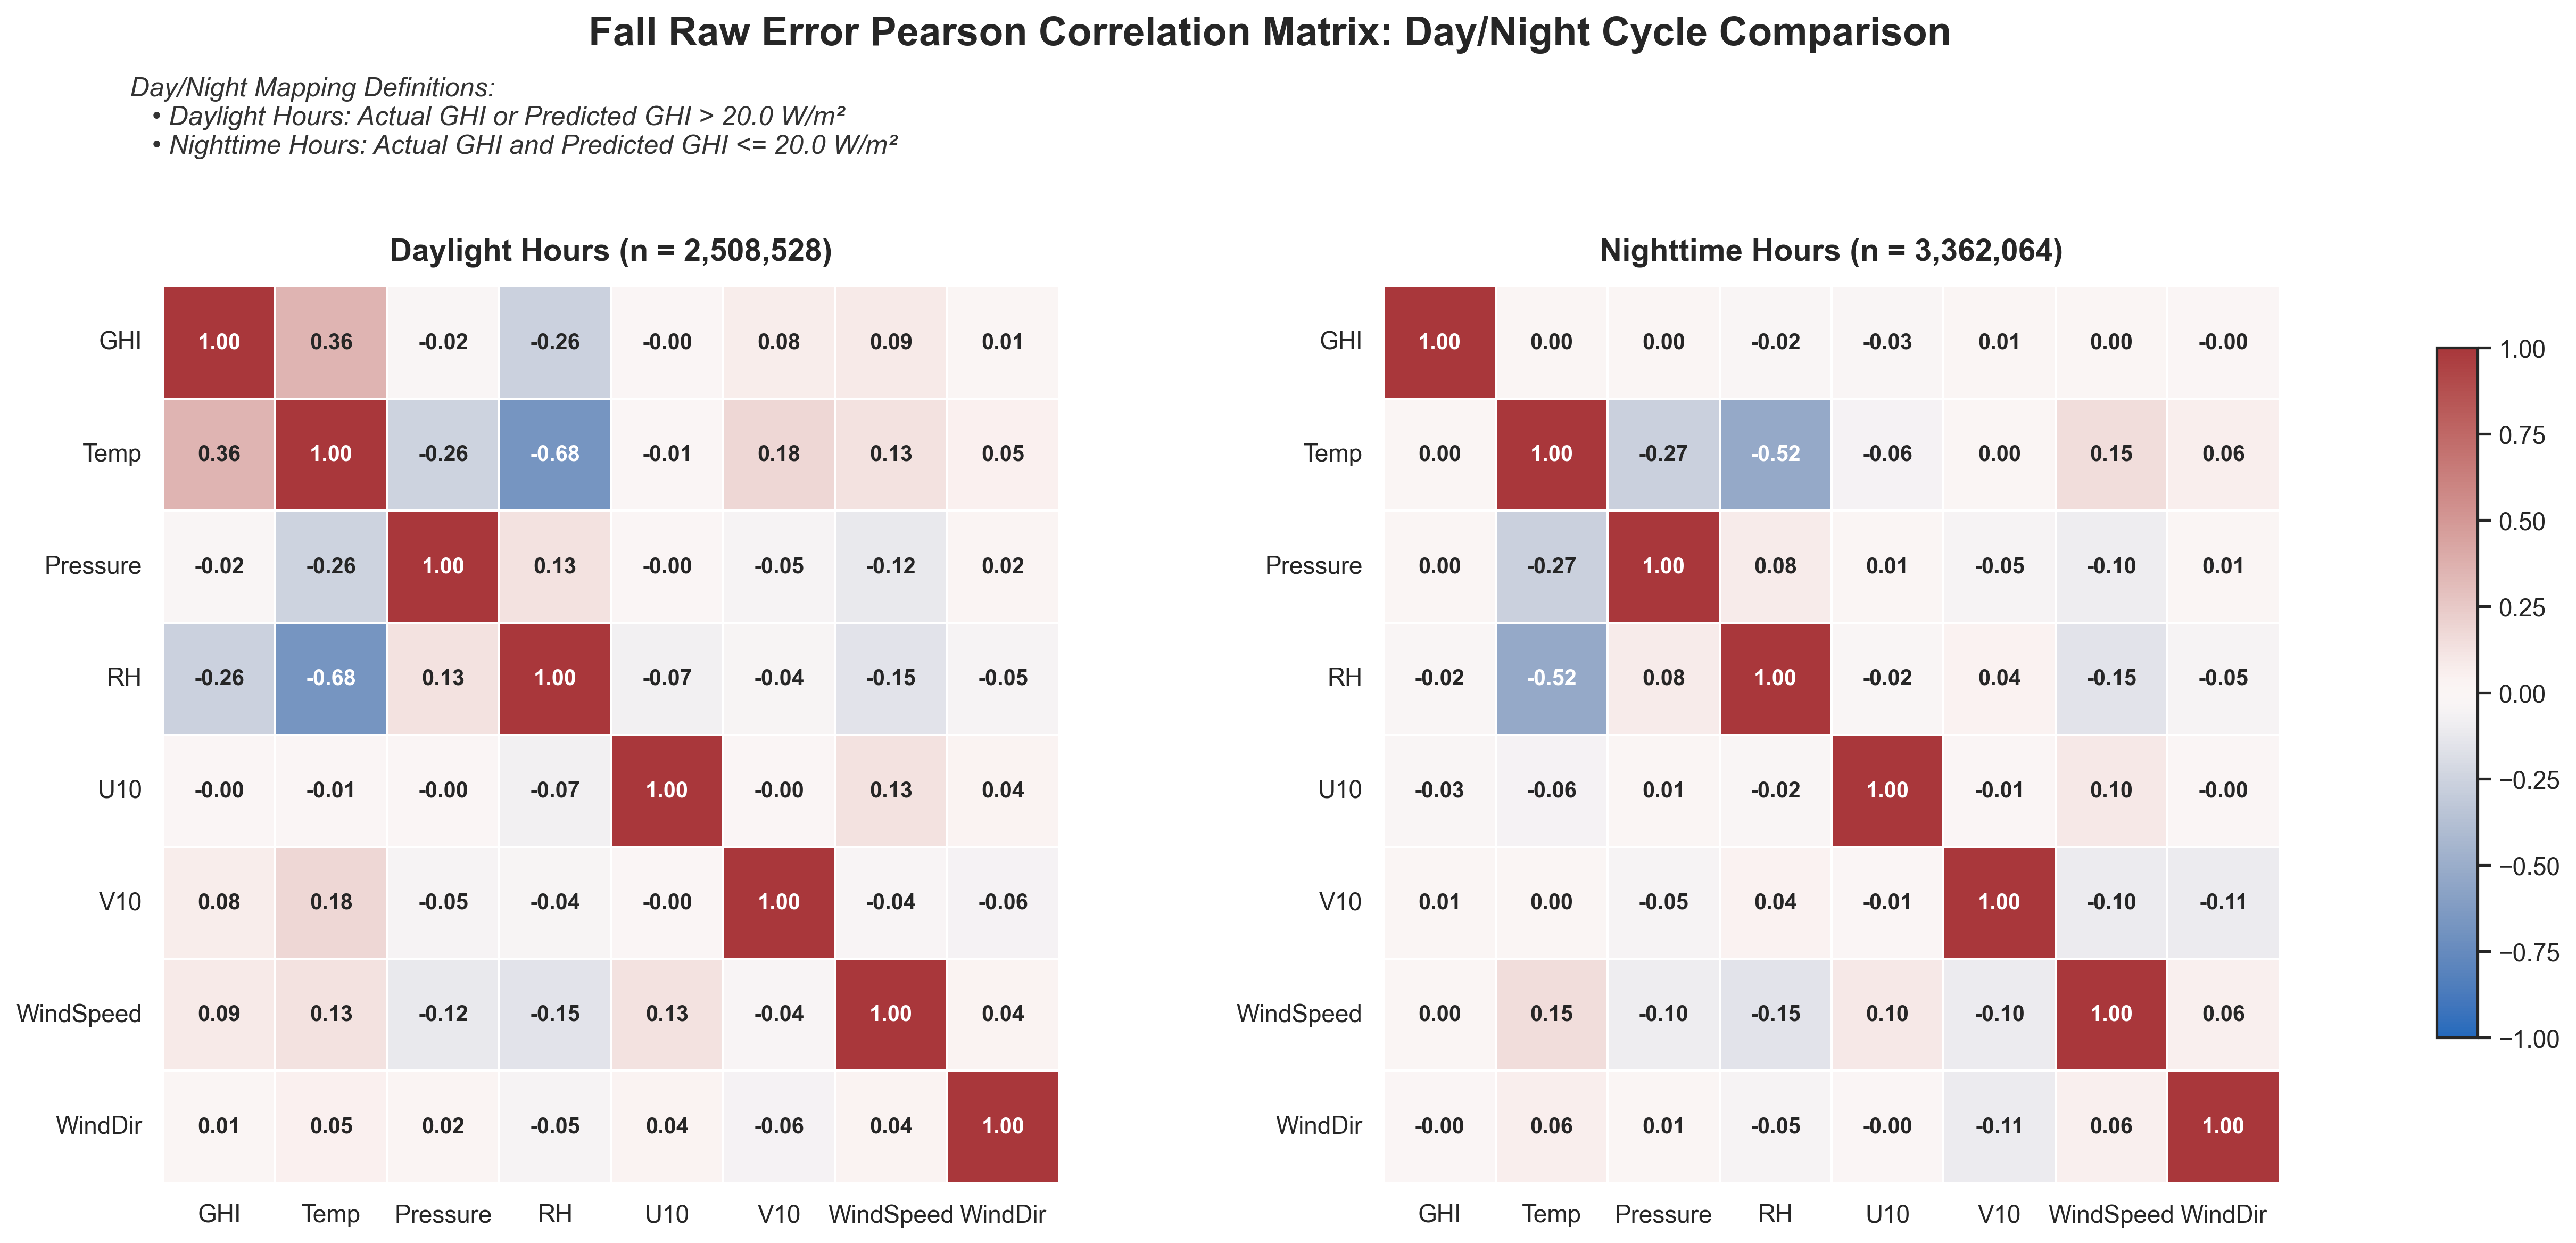
\includegraphics[width=\textwidth]{figures/Q7/SEASONS/correlation_heatmap_fall_diurnal_comparison.png}
  \caption{Fall Raw Error Pearson Correlation Matrix: Daylight Hours ($n = 2,508,528$, left) versus Nighttime Hours ($n = 3,362,064$, right) comparison.}
  \label{fig:app_fall_day_night}
\end{figure}

% --- INTERANNUAL VARIATIONS ---
\begin{figure}[H]
  \centering
  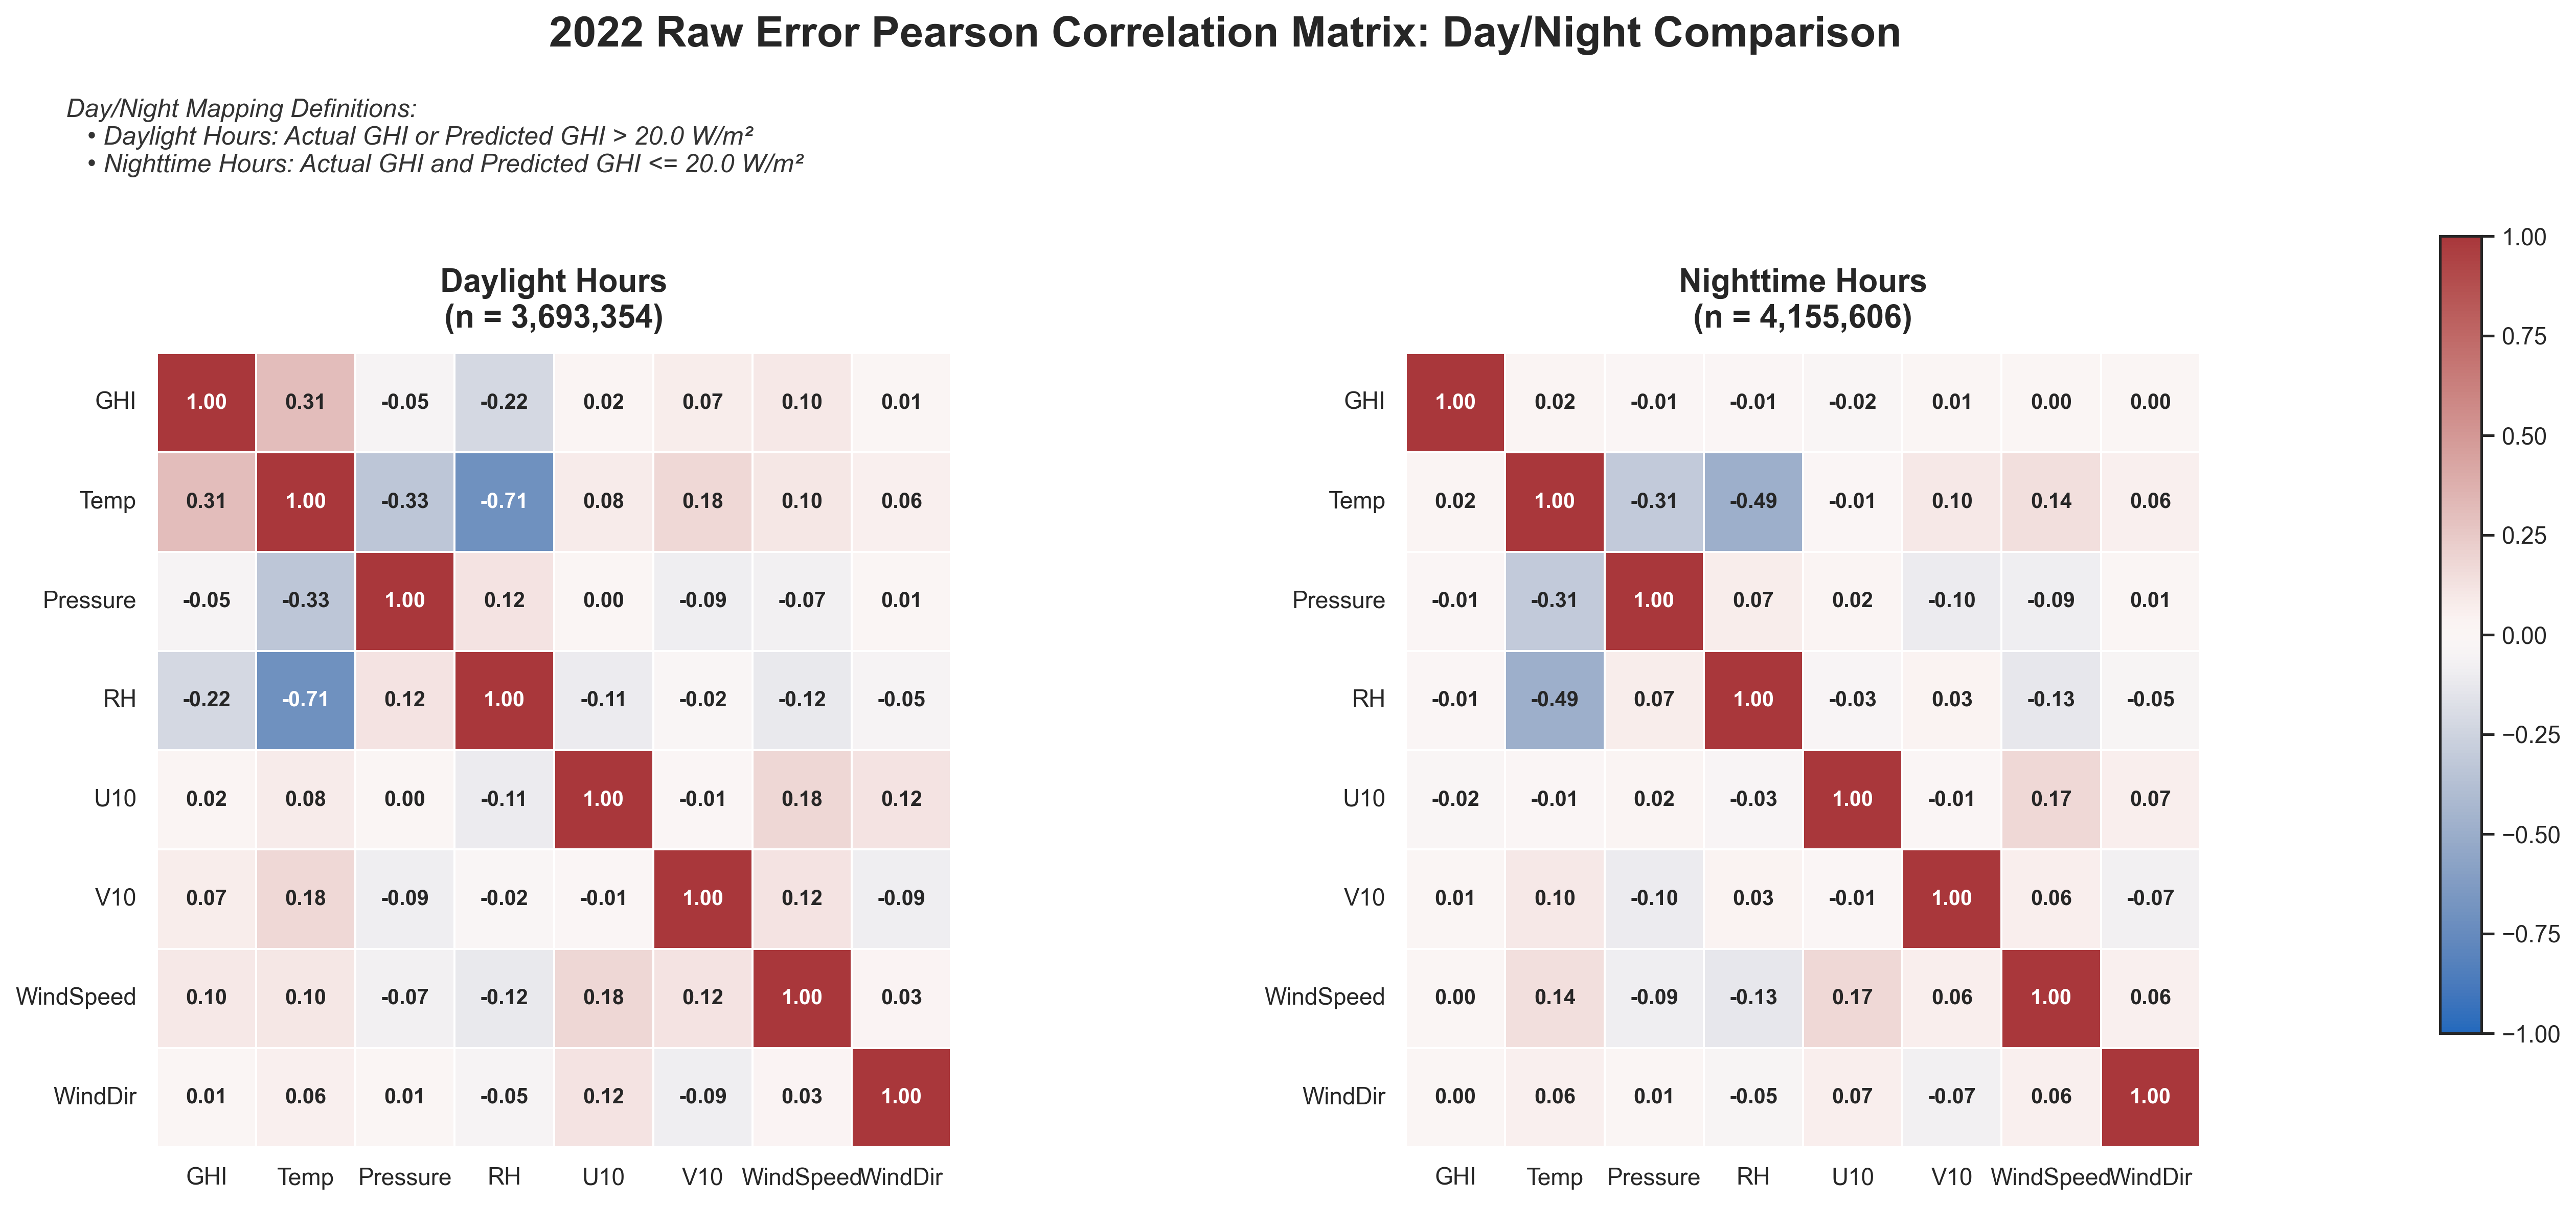
\includegraphics[width=\textwidth]{figures/Q7/YEARS/annual_corr_diurnal_split_2022.png}
  \caption{2022 Raw Error Pearson Correlation Matrix: Daylight Hours ($n = 3,693,554$, left) versus Nighttime Hours ($n = 4,155,606$, right) comparison.}
  \label{fig:app_corr_2022}
\end{figure}

\begin{figure}[H]
  \centering
  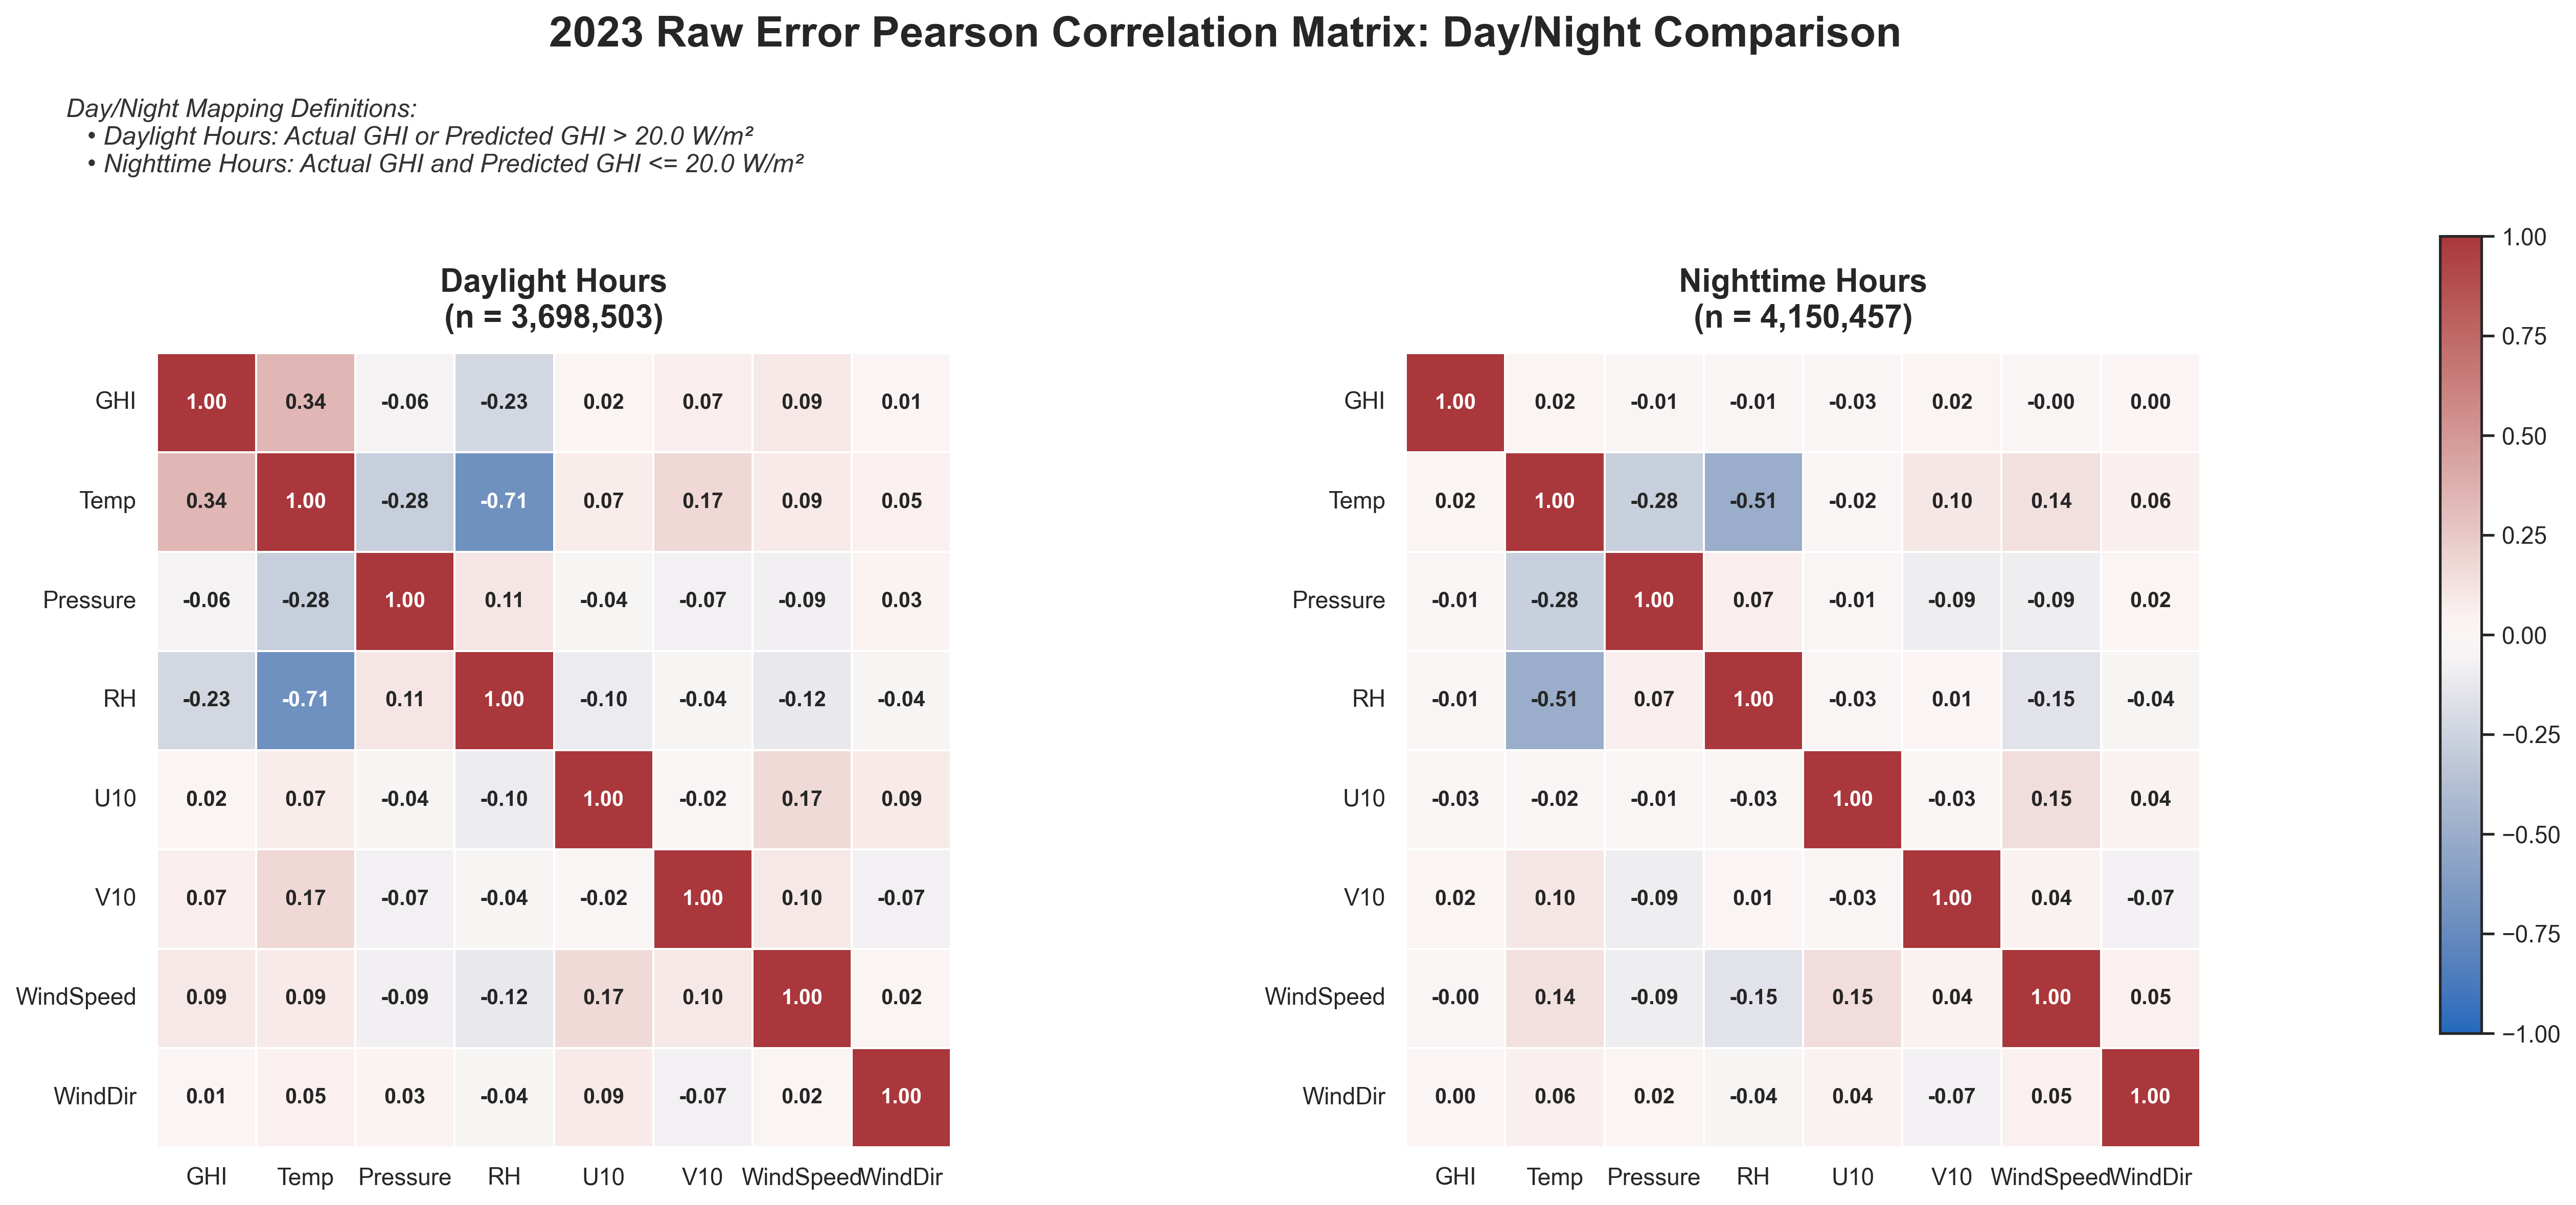
\includegraphics[width=\textwidth]{figures/Q7/YEARS/annual_corr_diurnal_split_2023.png}
  \caption{2023 Raw Error Pearson Correlation Matrix: Daylight Hours ($n = 3,698,503$, left) versus Nighttime Hours ($n = 4,150,457$, right) comparison.}
  \label{fig:app_corr_2023}
\end{figure}

\begin{figure}[H]
  \centering
  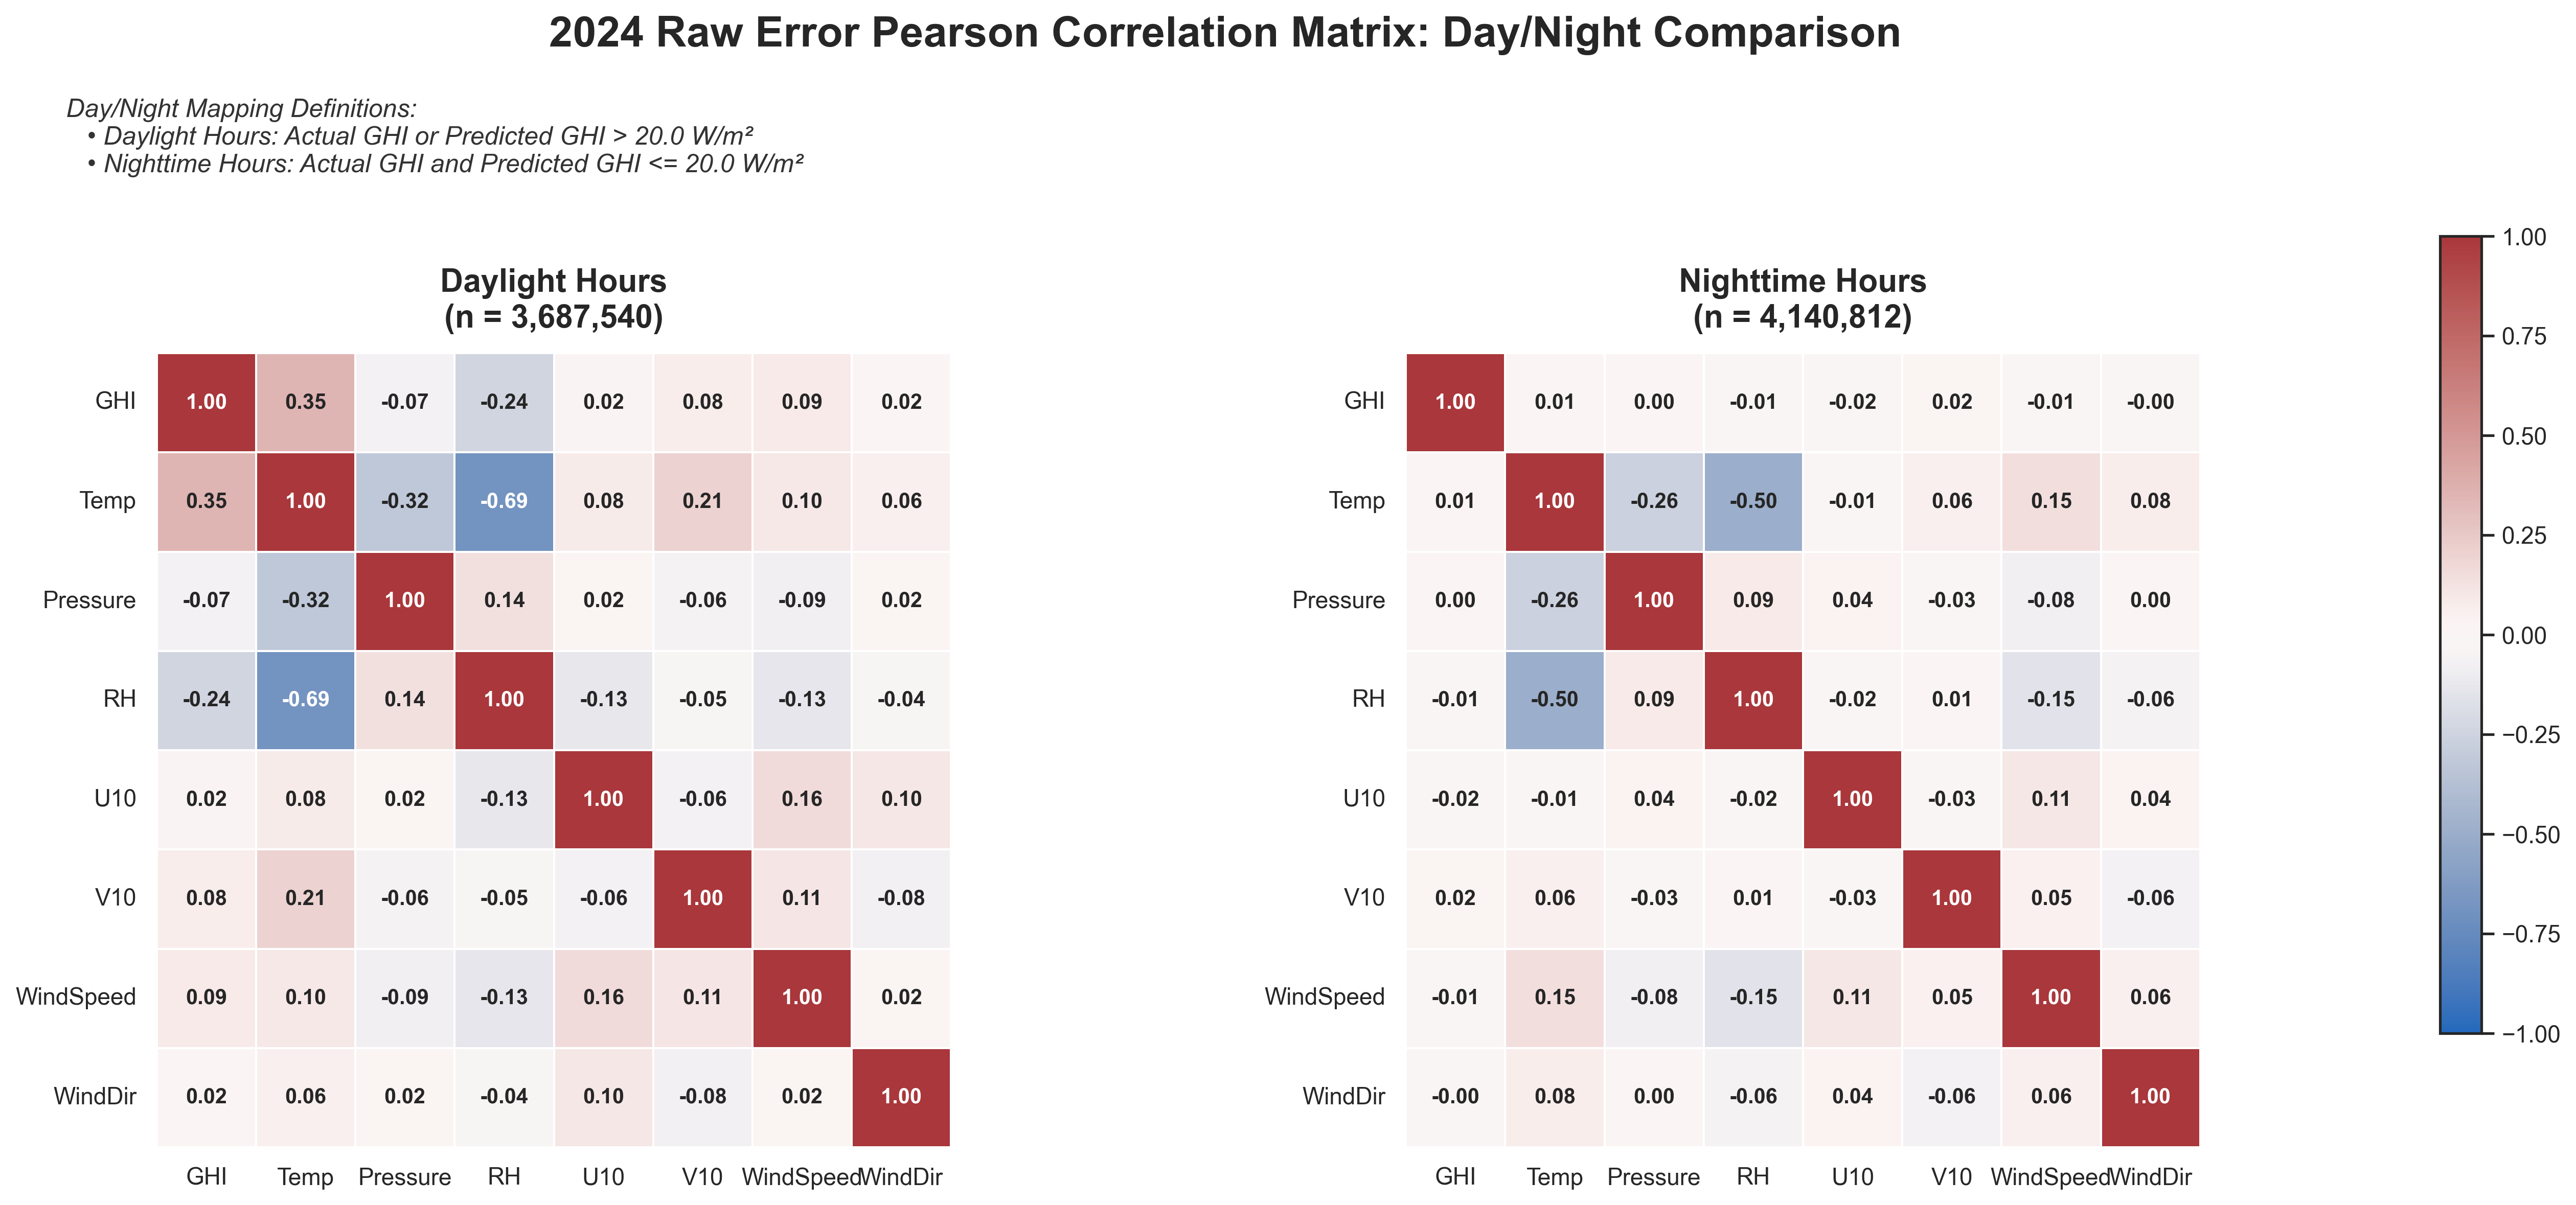
\includegraphics[width=\textwidth]{figures/Q7/YEARS/annual_corr_diurnal_split_2024.png}
  \caption{2024 Raw Error Pearson Correlation Matrix: Daylight Hours ($n = 3,687,540$, left) versus Nighttime Hours ($n = 4,140,812$, right) comparison.}
  \label{fig:app_corr_2024}
\end{figure}

% --- REGIONAL / ZONAL VARIATIONS ---
\begin{figure}[H]
  \centering
  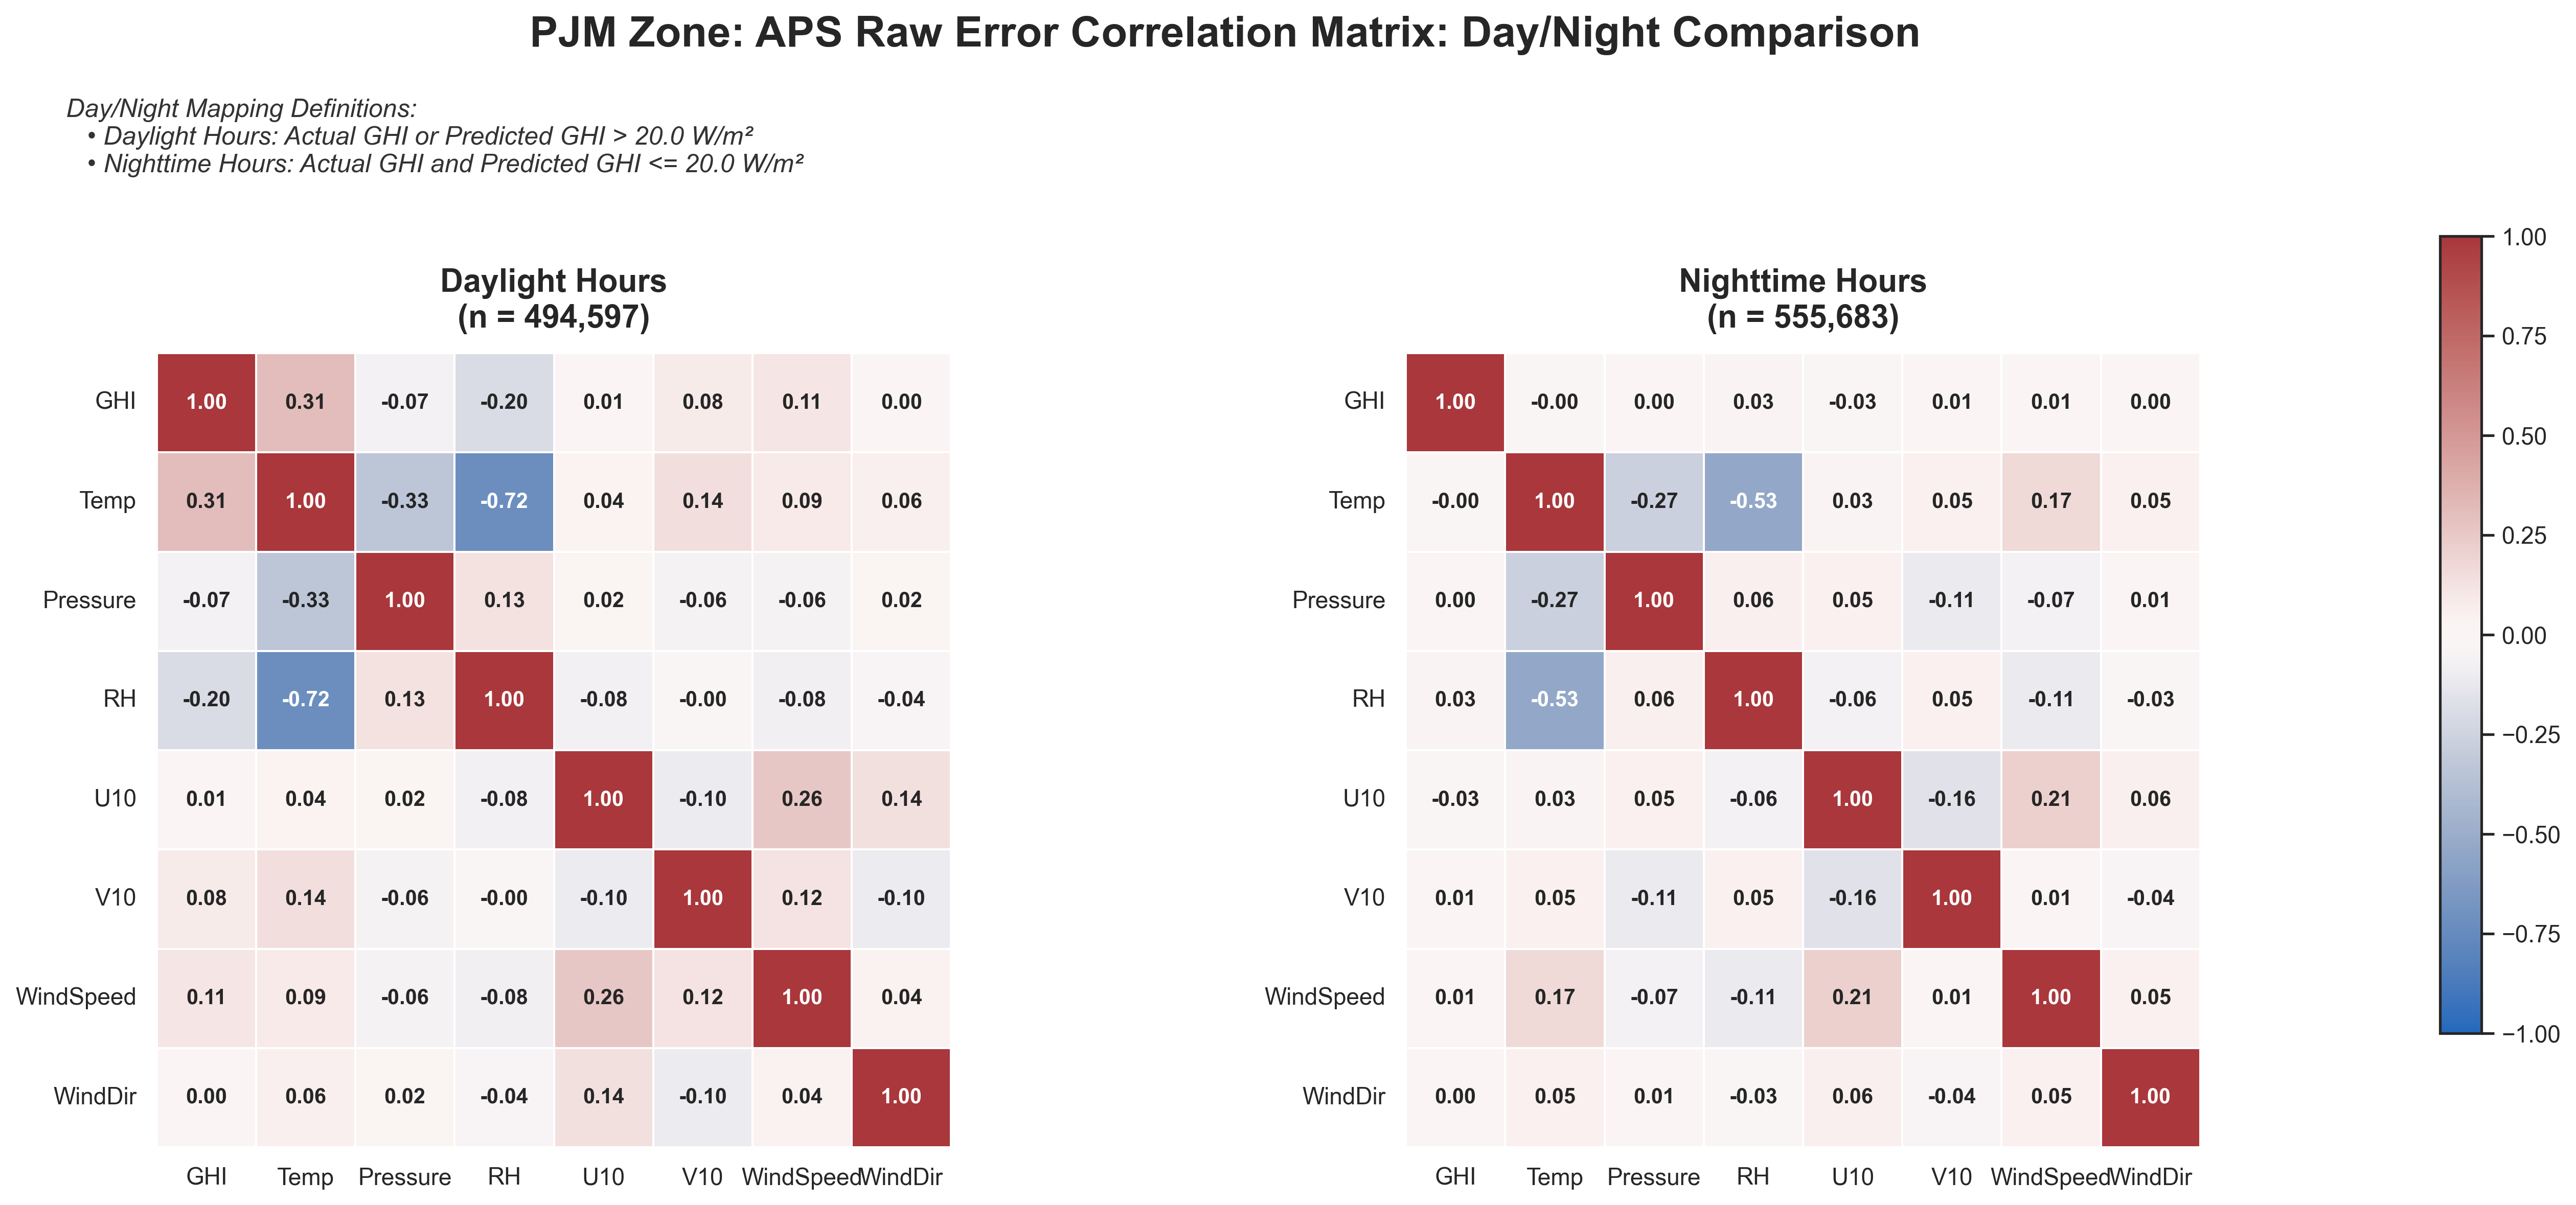
\includegraphics[width=\textwidth]{figures/Q7/ZONES/zone_corr_diurnal_split_aps.png}
  \caption{Cross-variable error matrices computed independently across major PJM transmission zones.}
  \label{fig:app_zone_aps}
\end{figure}

\begin{figure}[H]
  \centering
  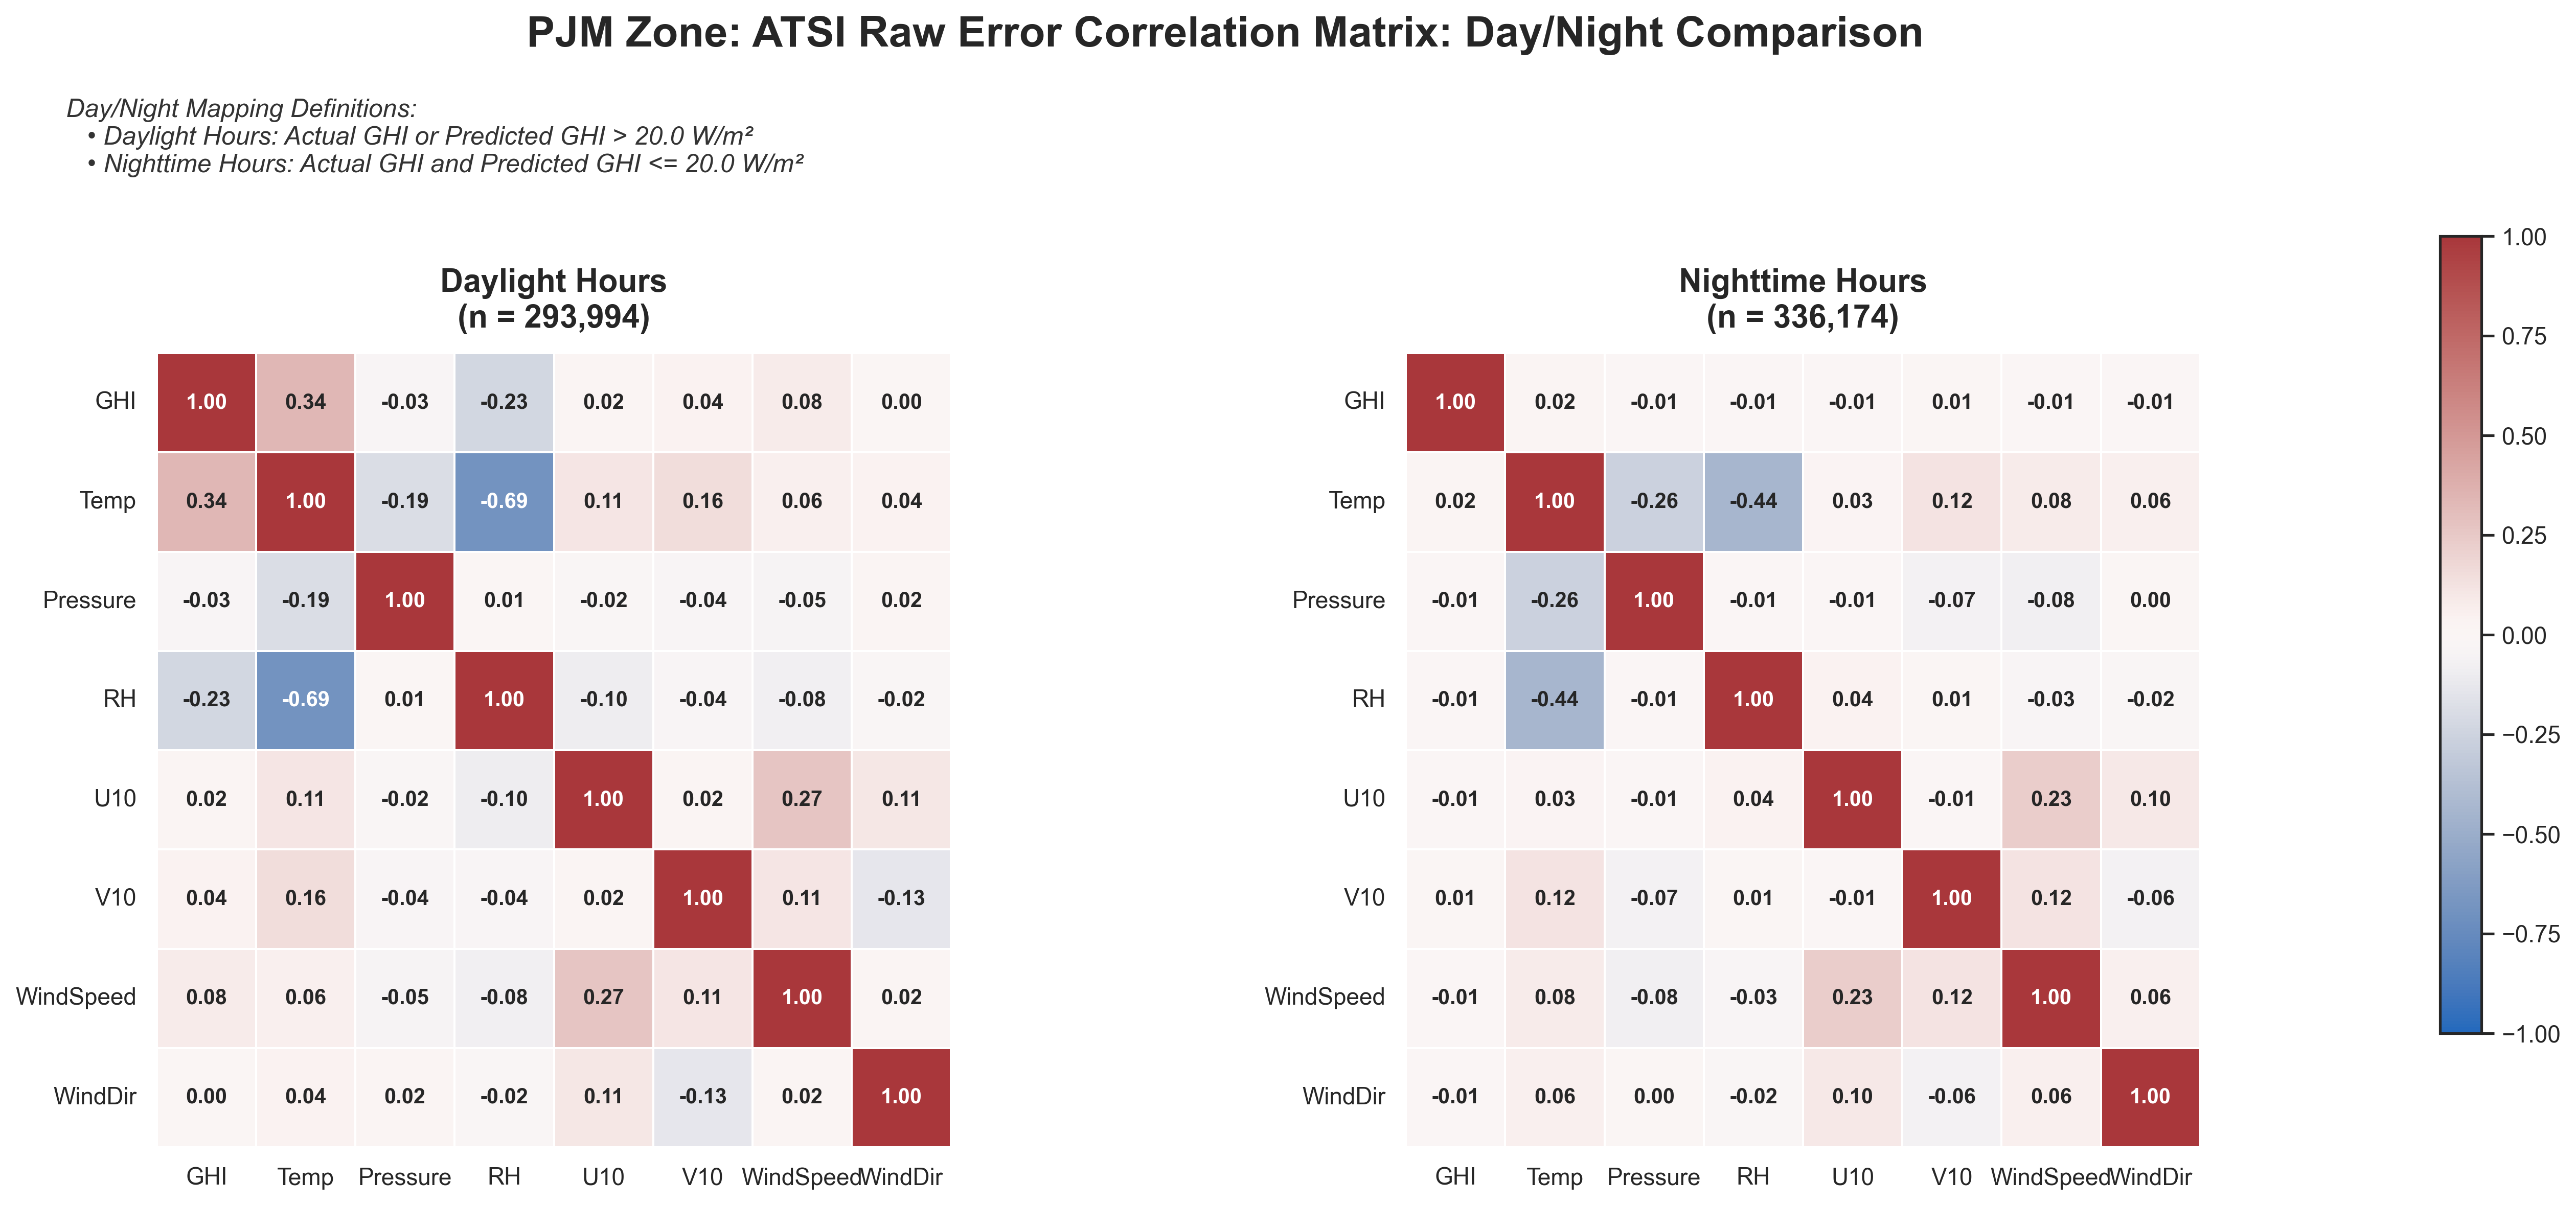
\includegraphics[width=\textwidth]{figures/Q7/ZONES/zone_corr_diurnal_split_atsi.png}
  \caption{Cross-variable error matrices computed independently across major PJM transmission zones.}
  \label{fig:app_zone_atsi}
\end{figure}

\begin{figure}[H]
  \centering
  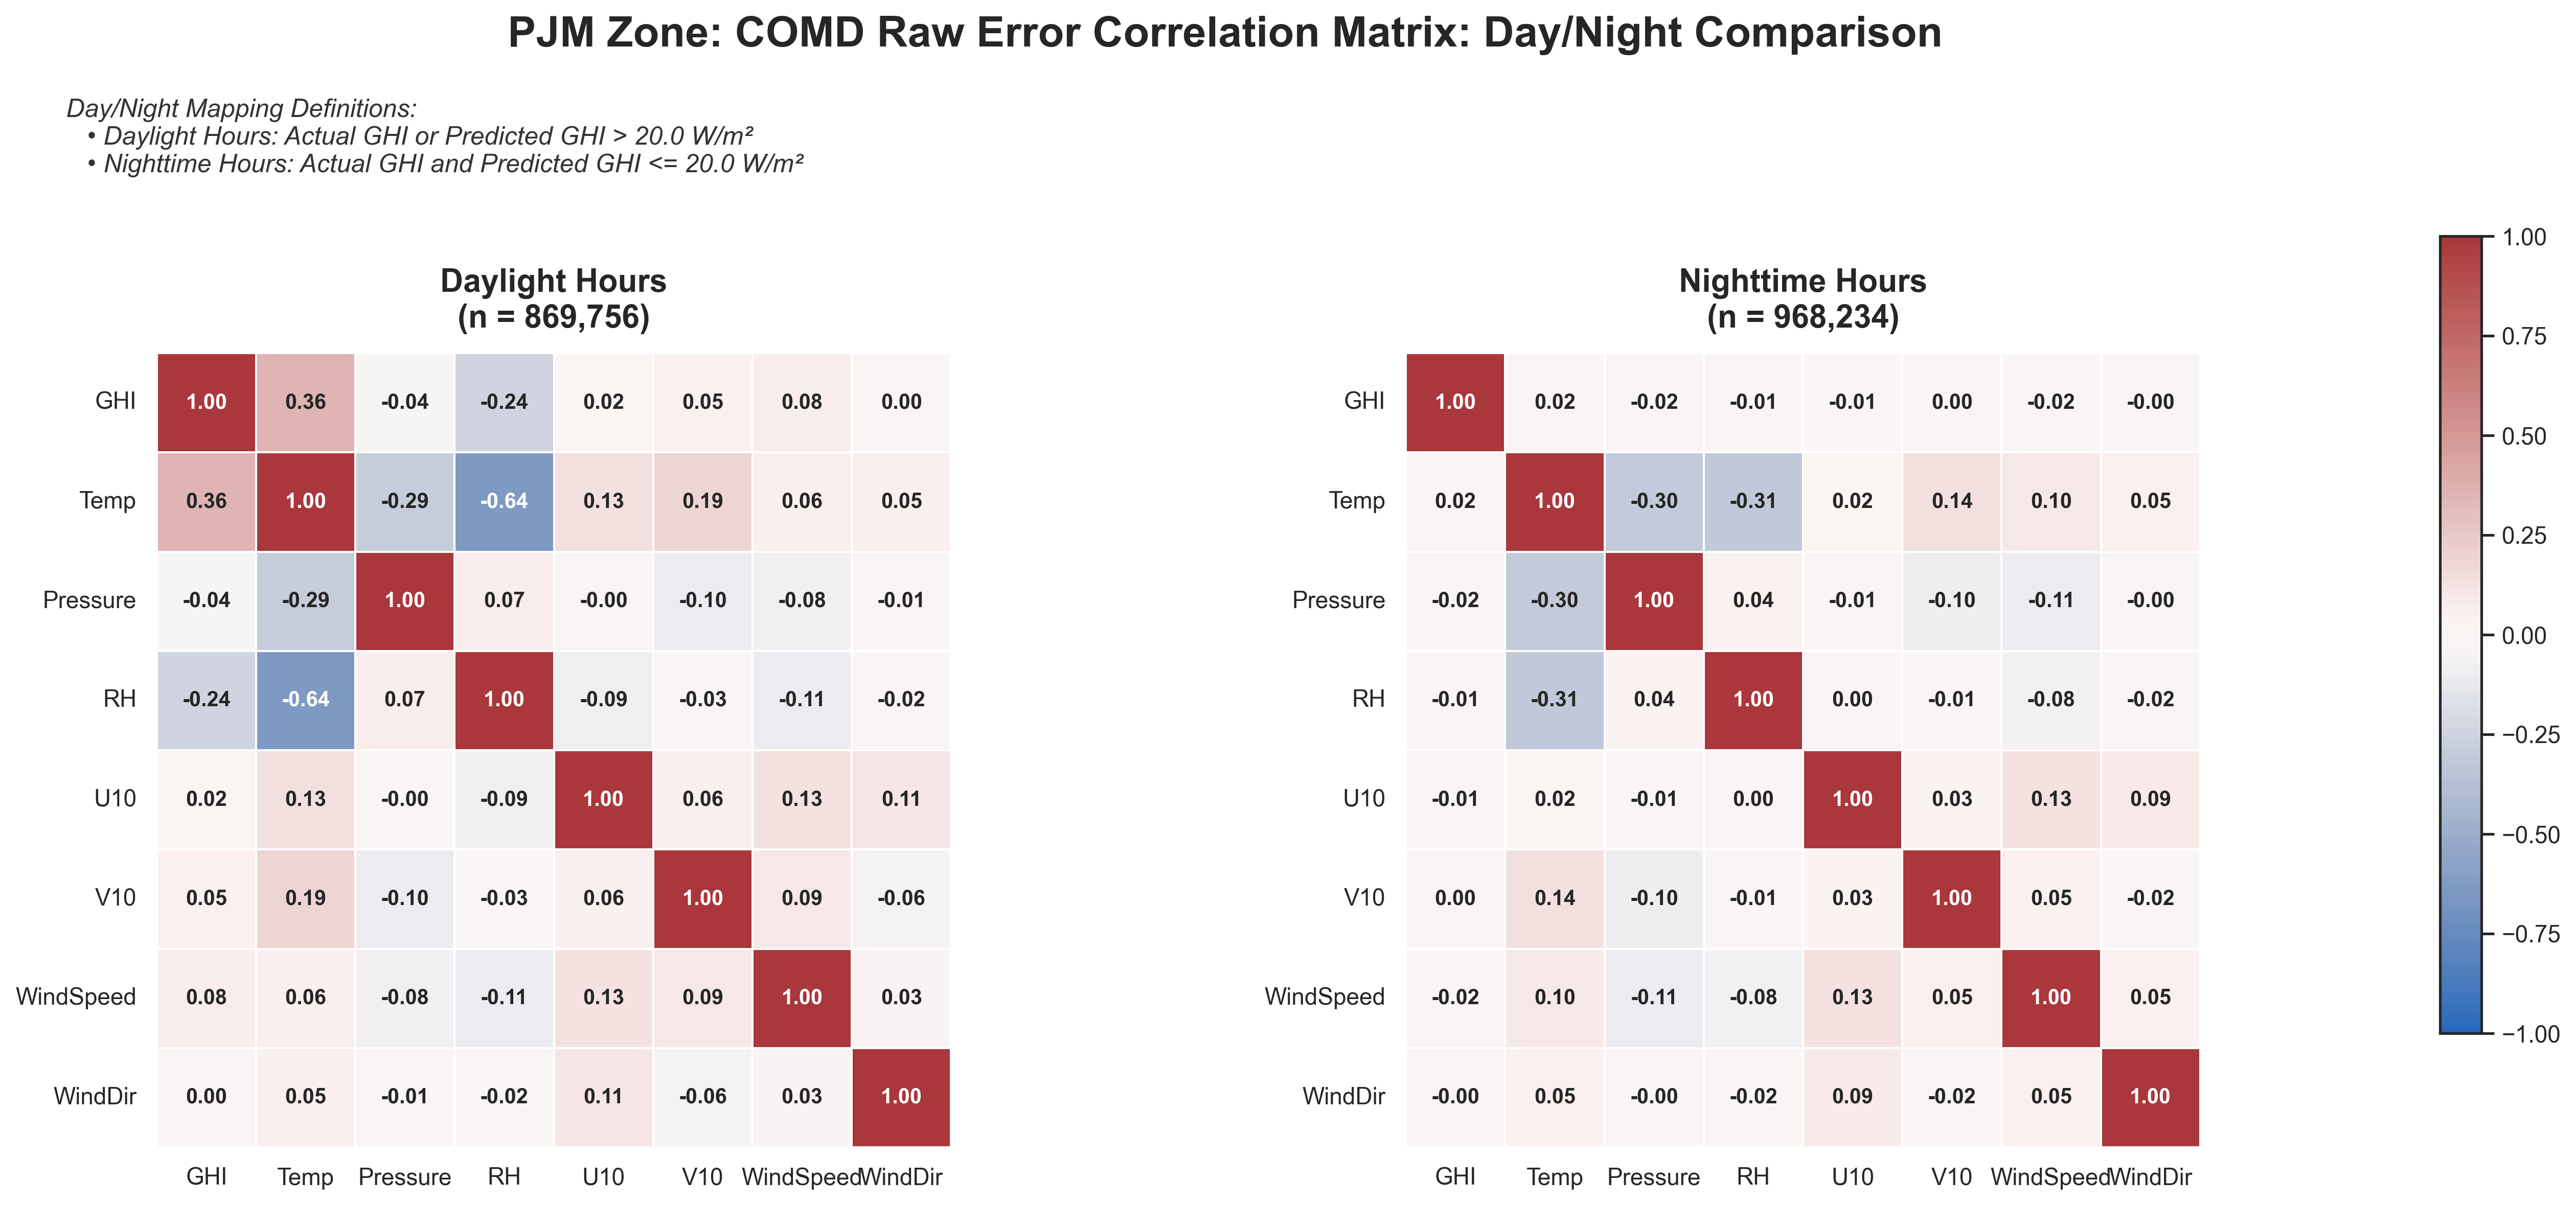
\includegraphics[width=\textwidth]{figures/Q7/ZONES/zone_corr_diurnal_split_comd.png}
  \caption{Cross-variable error matrices computed independently across major PJM transmission zones.}
  \label{fig:app_zone_comd}
\end{figure}

\begin{figure}[H]
  \centering
  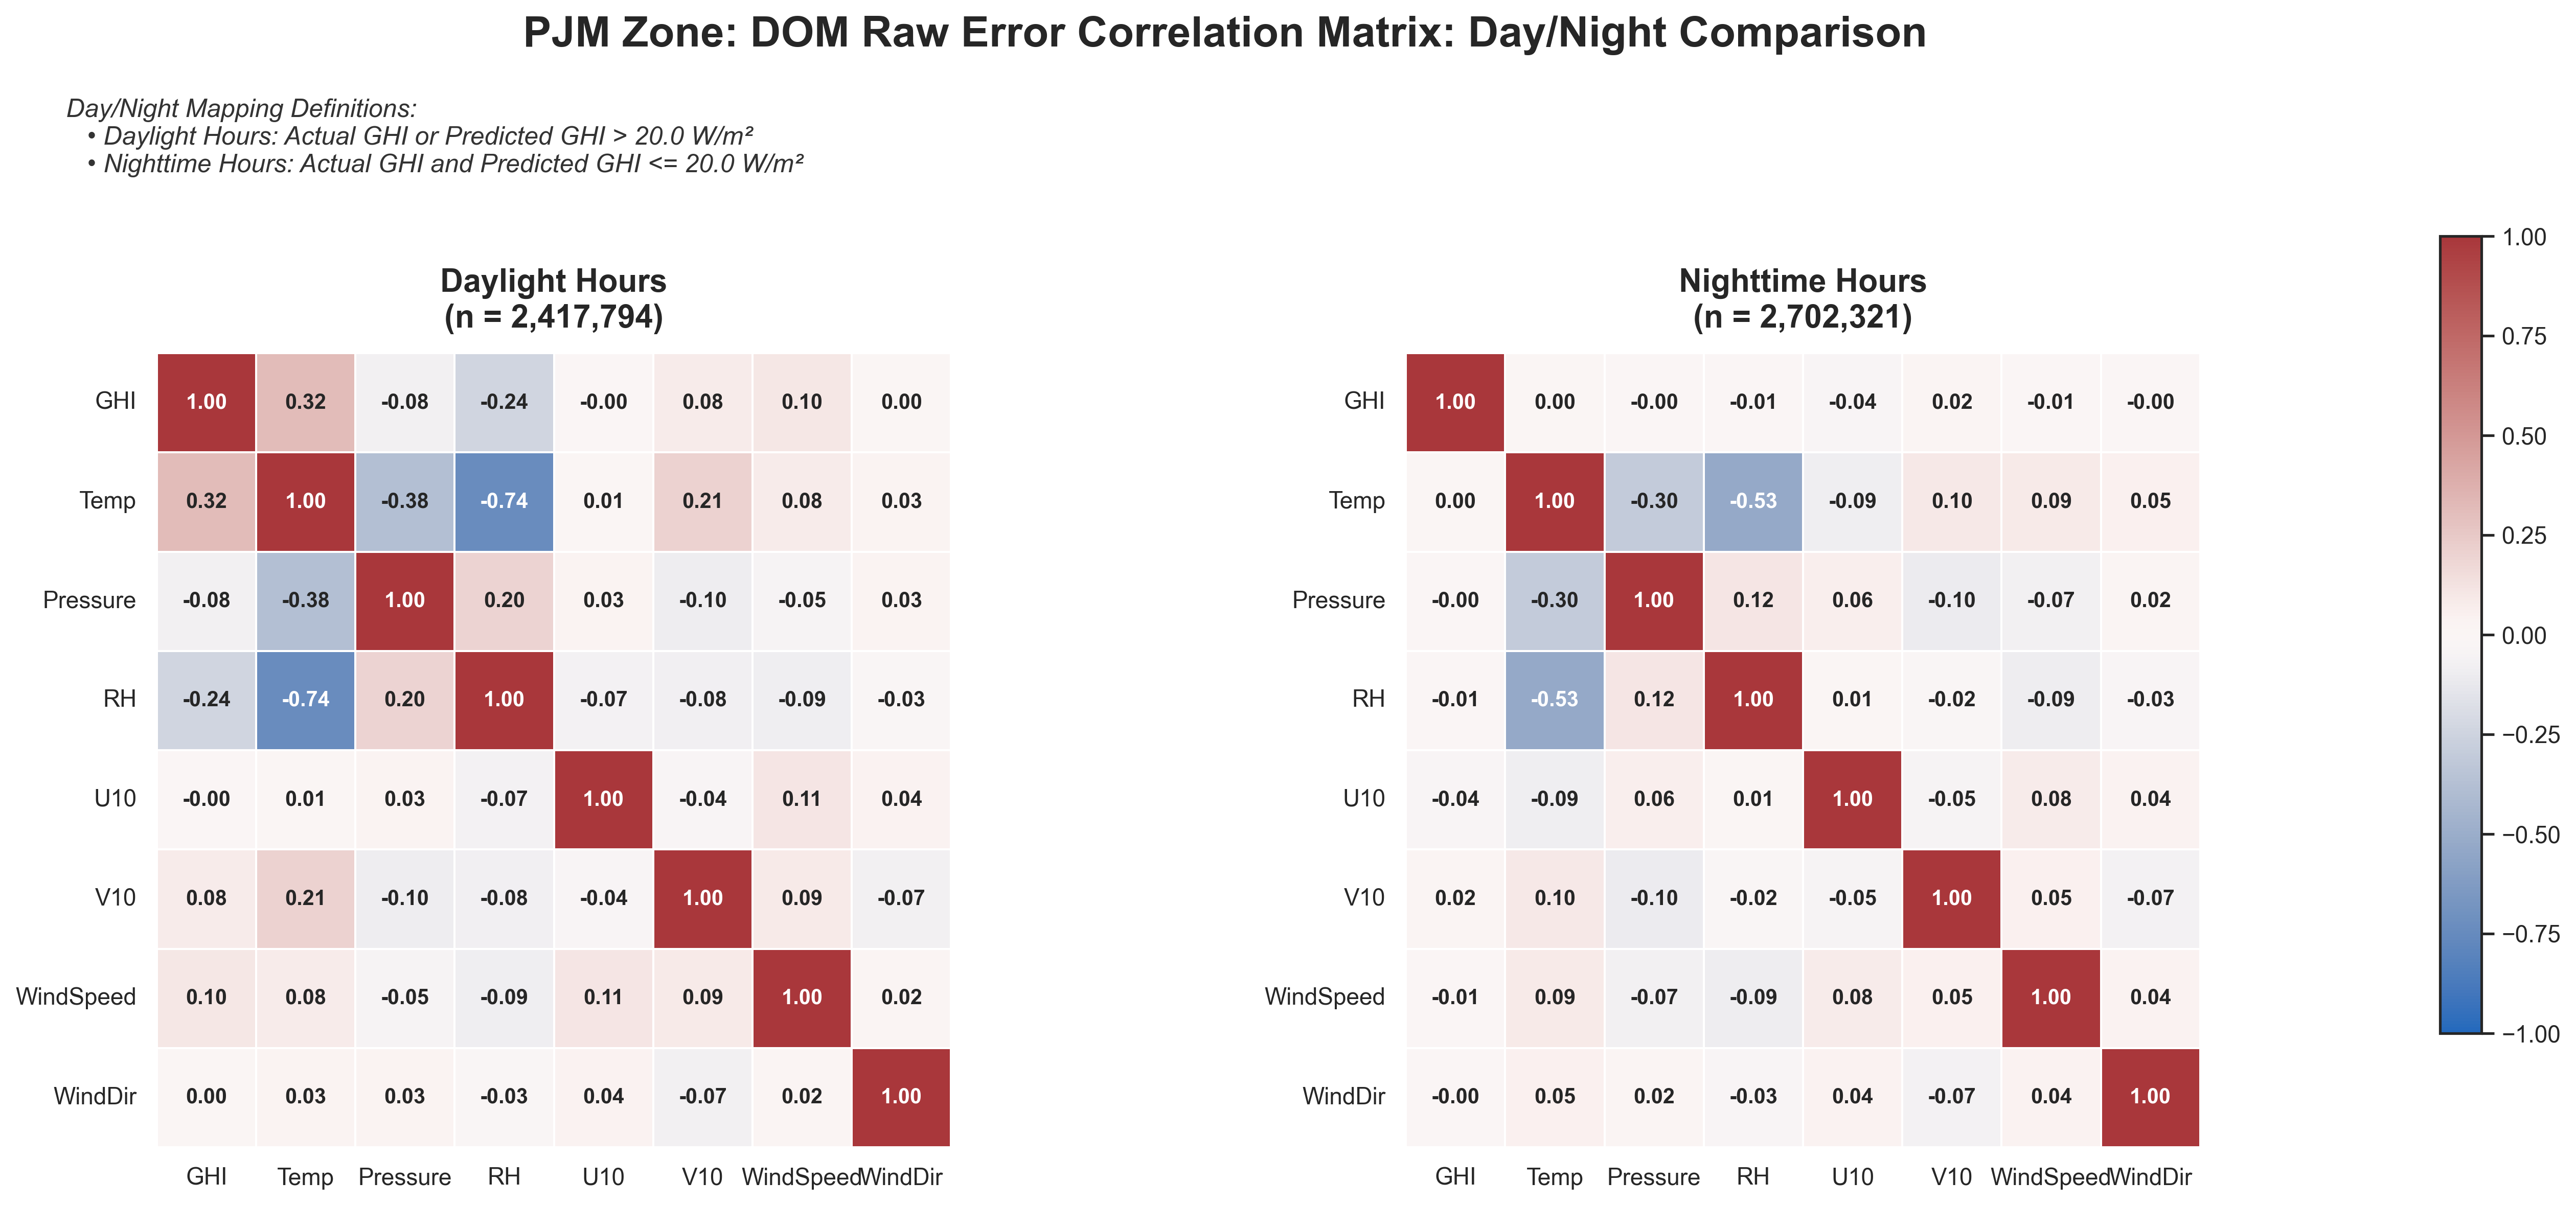
\includegraphics[width=\textwidth]{figures/Q7/ZONES/zone_corr_diurnal_split_dom.png}
  \caption{Cross-variable error matrices computed independently across major PJM transmission zones.}
  \label{fig:app_zone_dom}
\end{figure}

\begin{figure}[H]
  \centering
  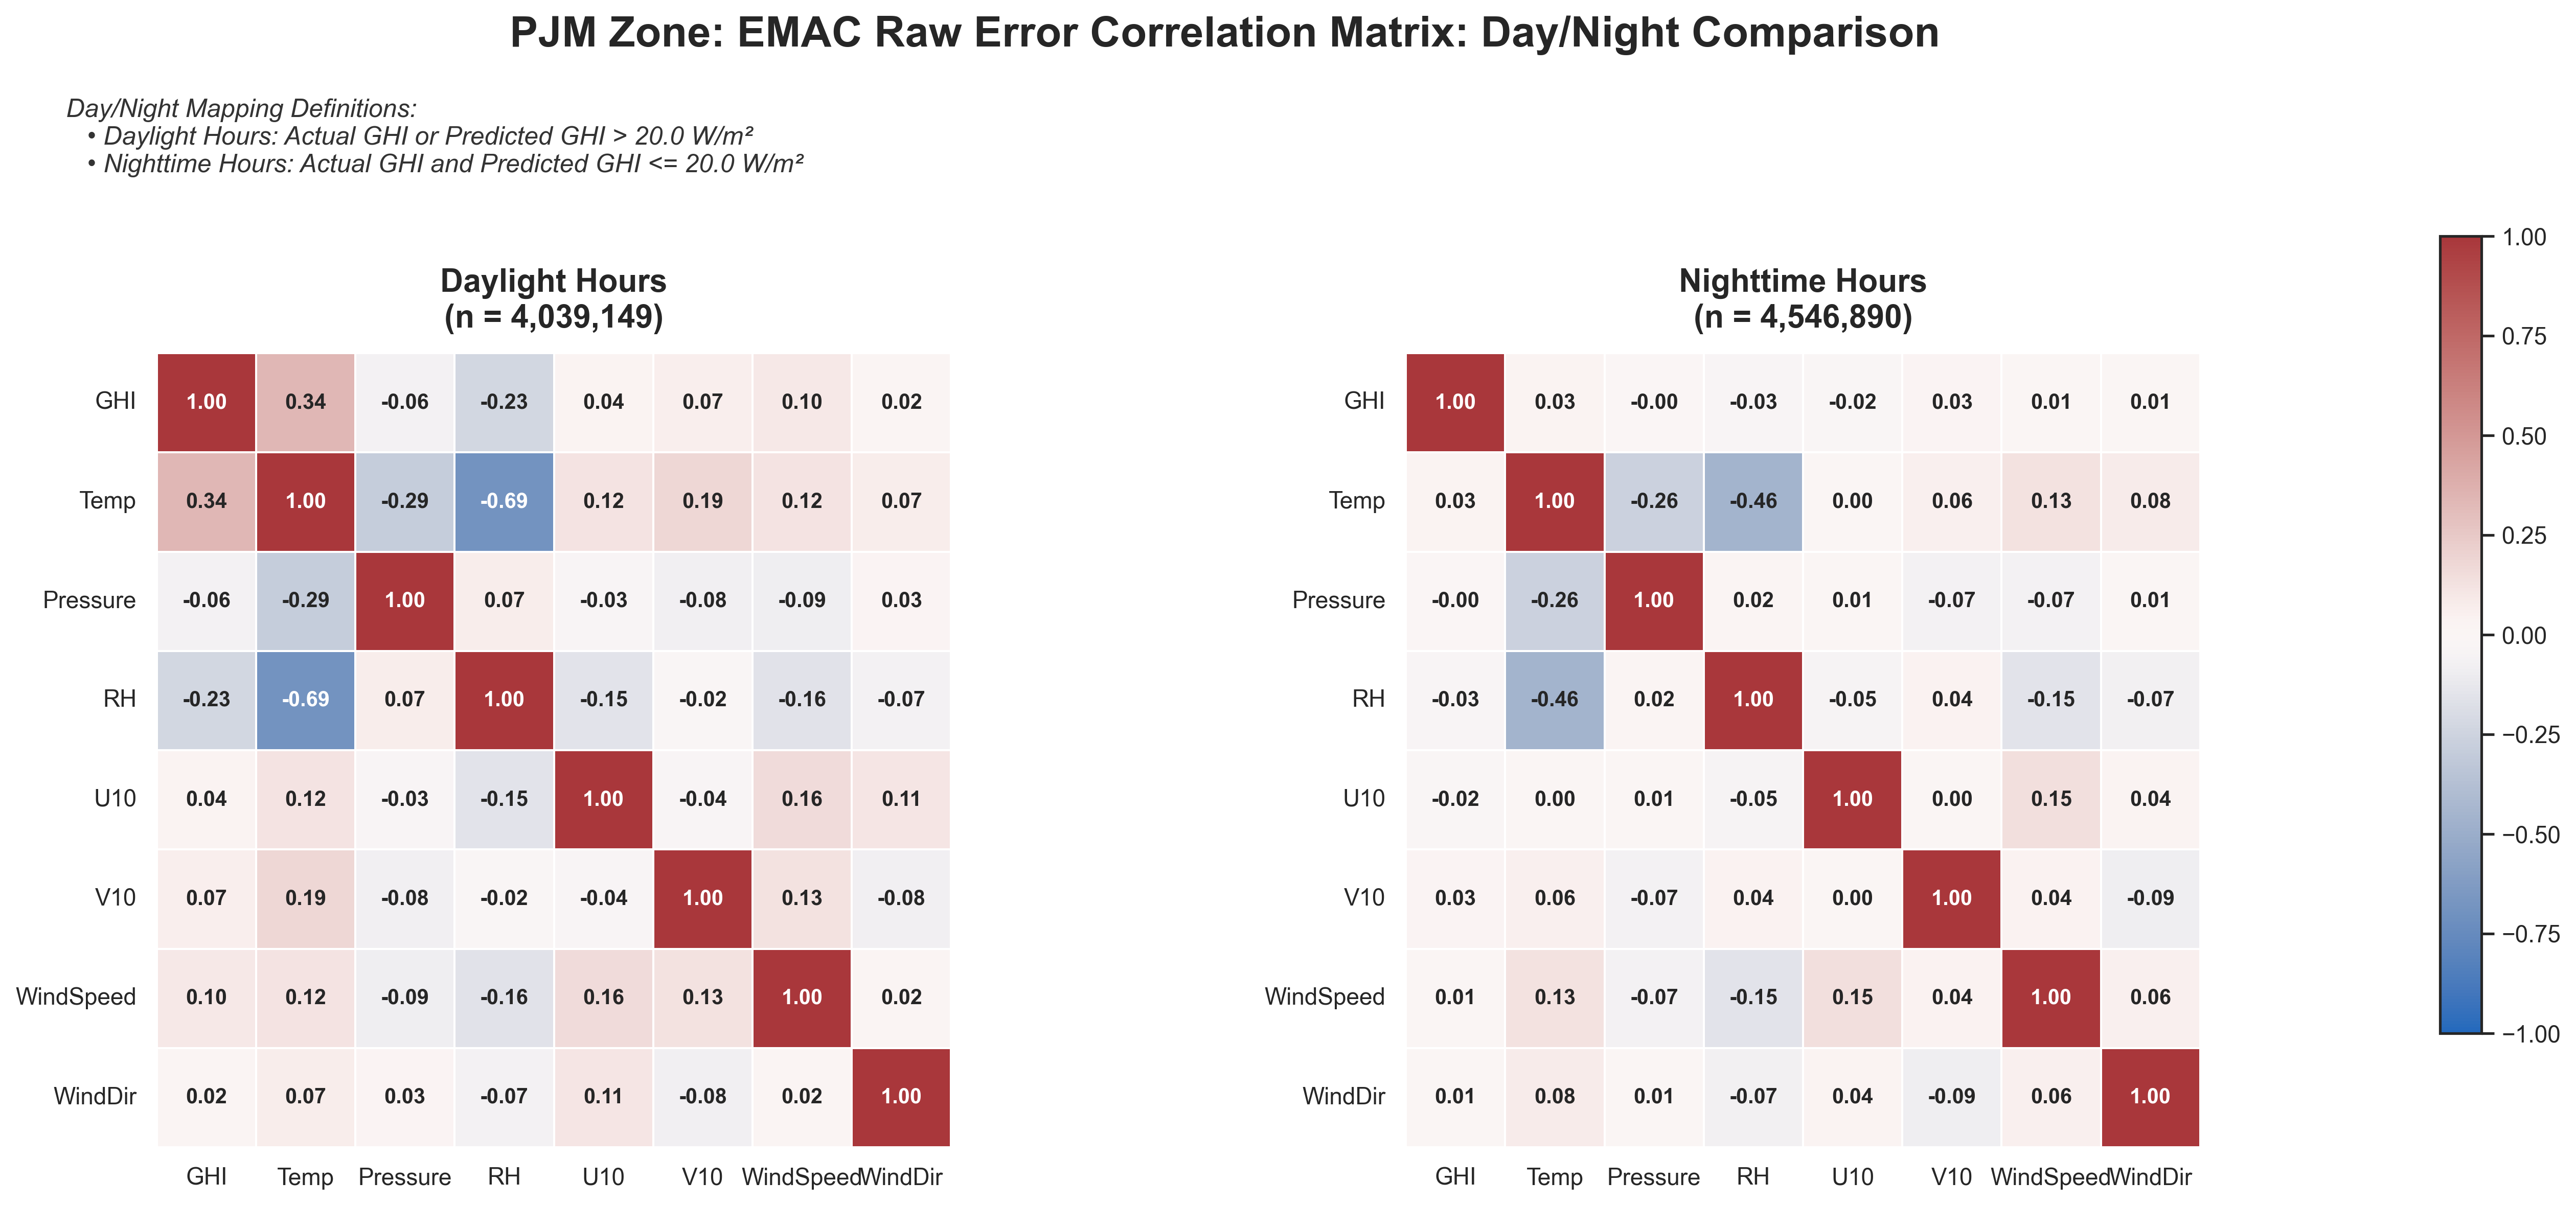
\includegraphics[width=\textwidth]{figures/Q7/ZONES/zone_corr_diurnal_split_emac.png}
  \caption{Cross-variable error matrices computed independently across major PJM transmission zones.}
  \label{fig:app_zone_emac}
\end{figure}

\begin{figure}[H]
  \centering
  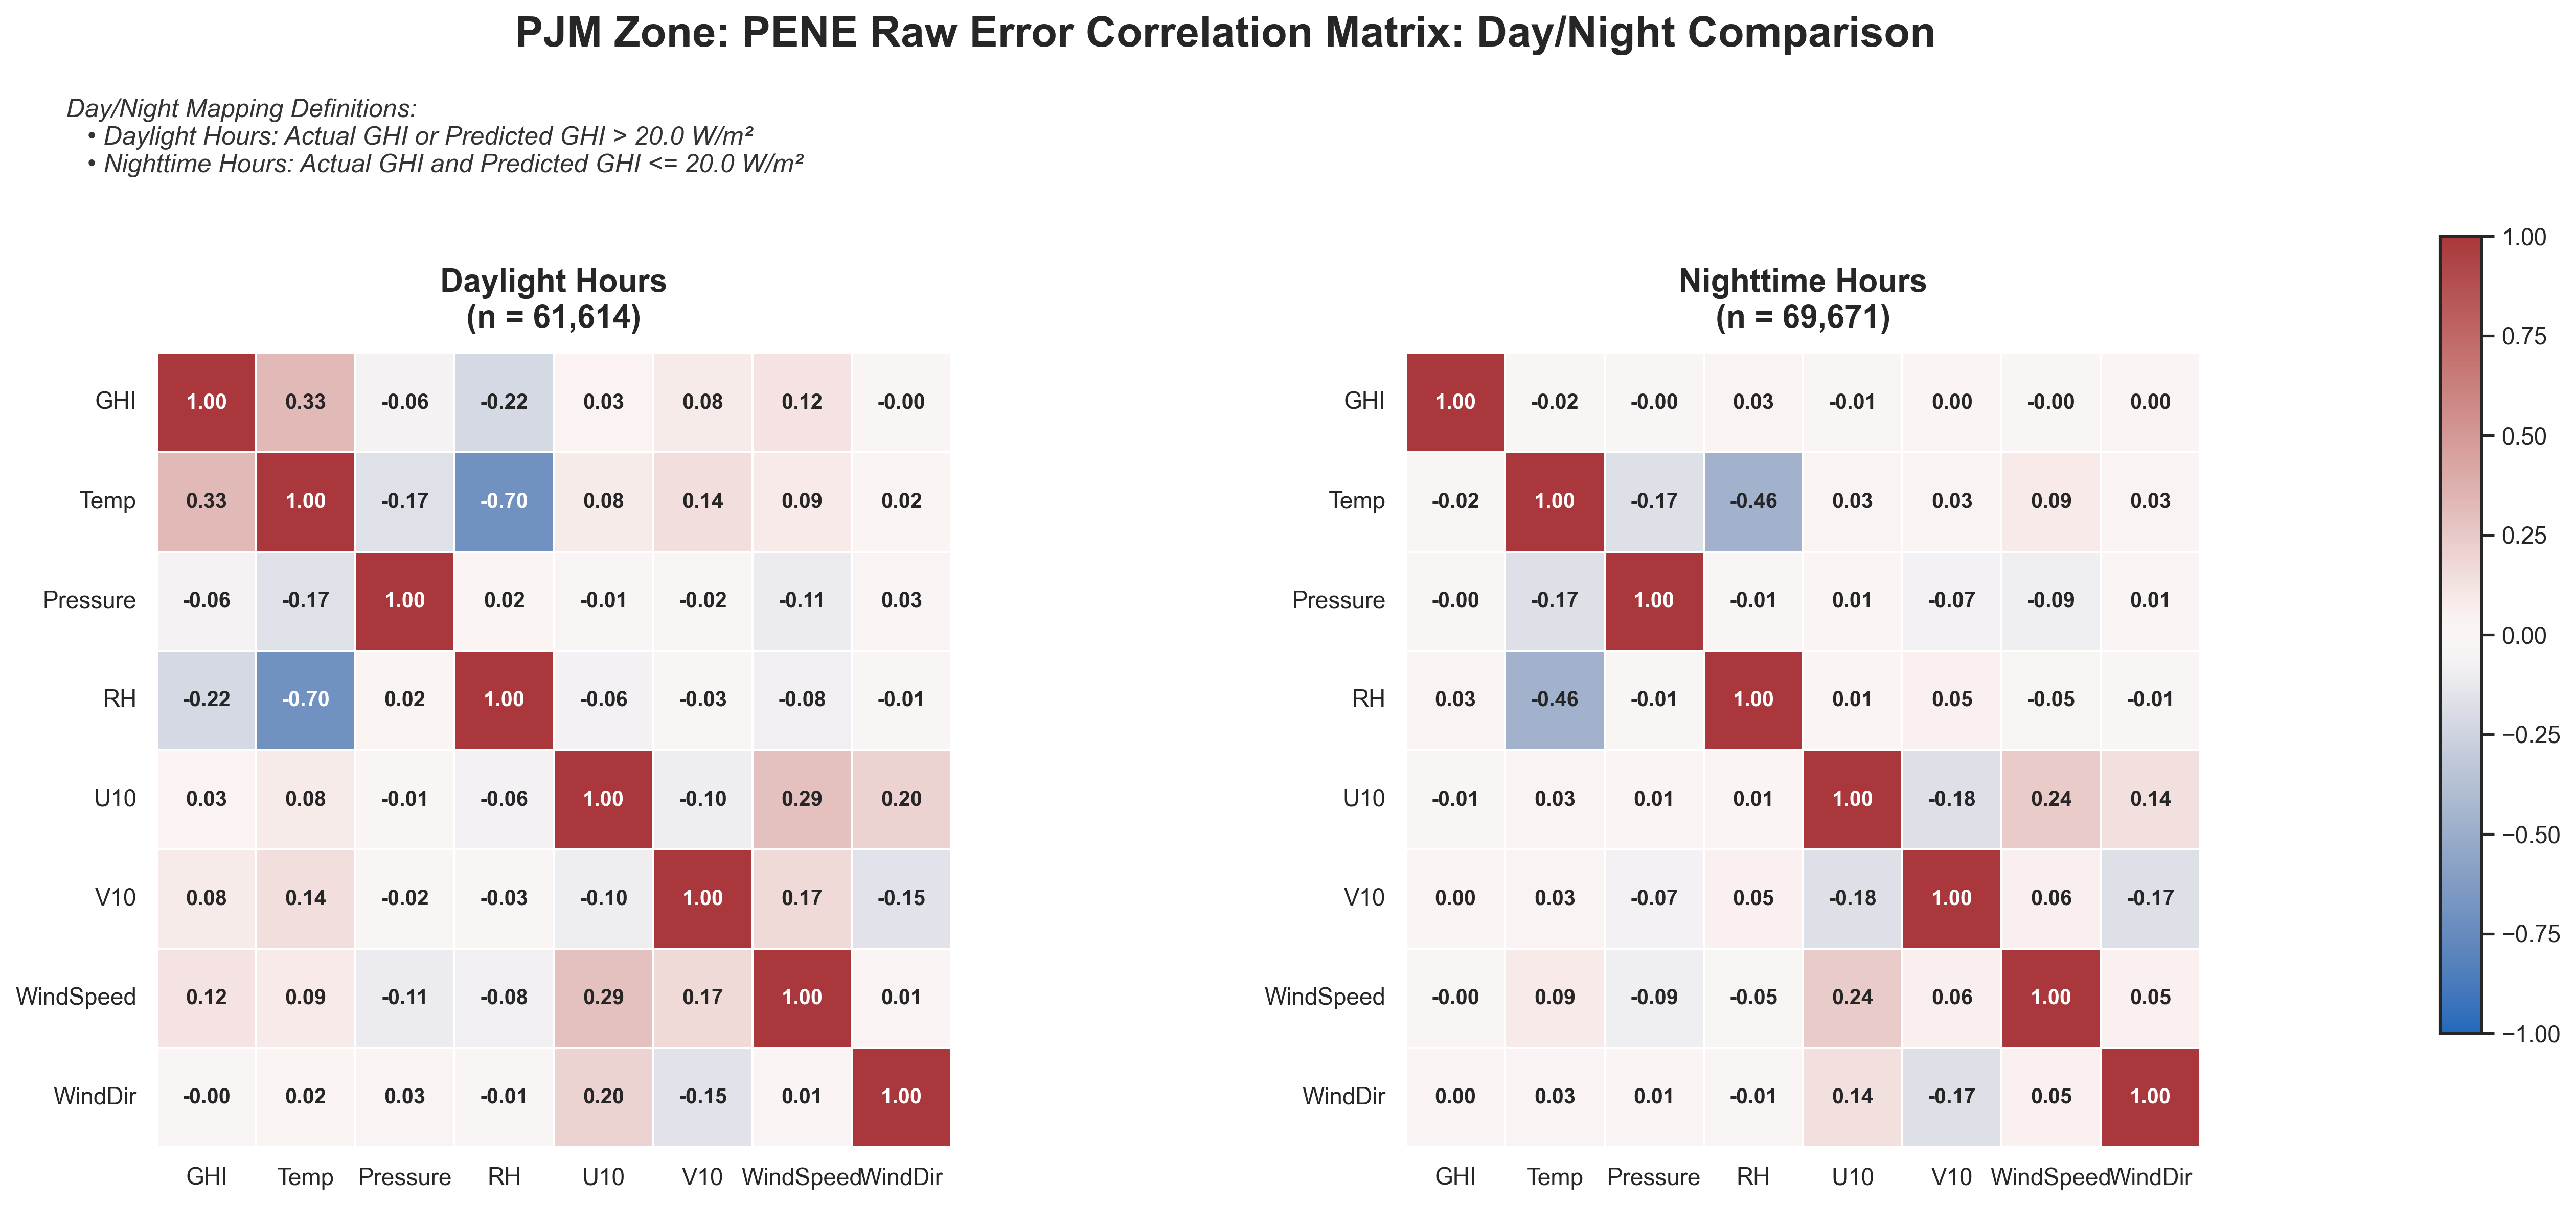
\includegraphics[width=\textwidth]{figures/Q7/ZONES/zone_corr_diurnal_split_pene.png}
  \caption{Cross-variable error matrices computed independently across major PJM transmission zones.}
  \label{fig:app_zone_pene}
\end{figure}

\begin{figure}[H]
  \centering
  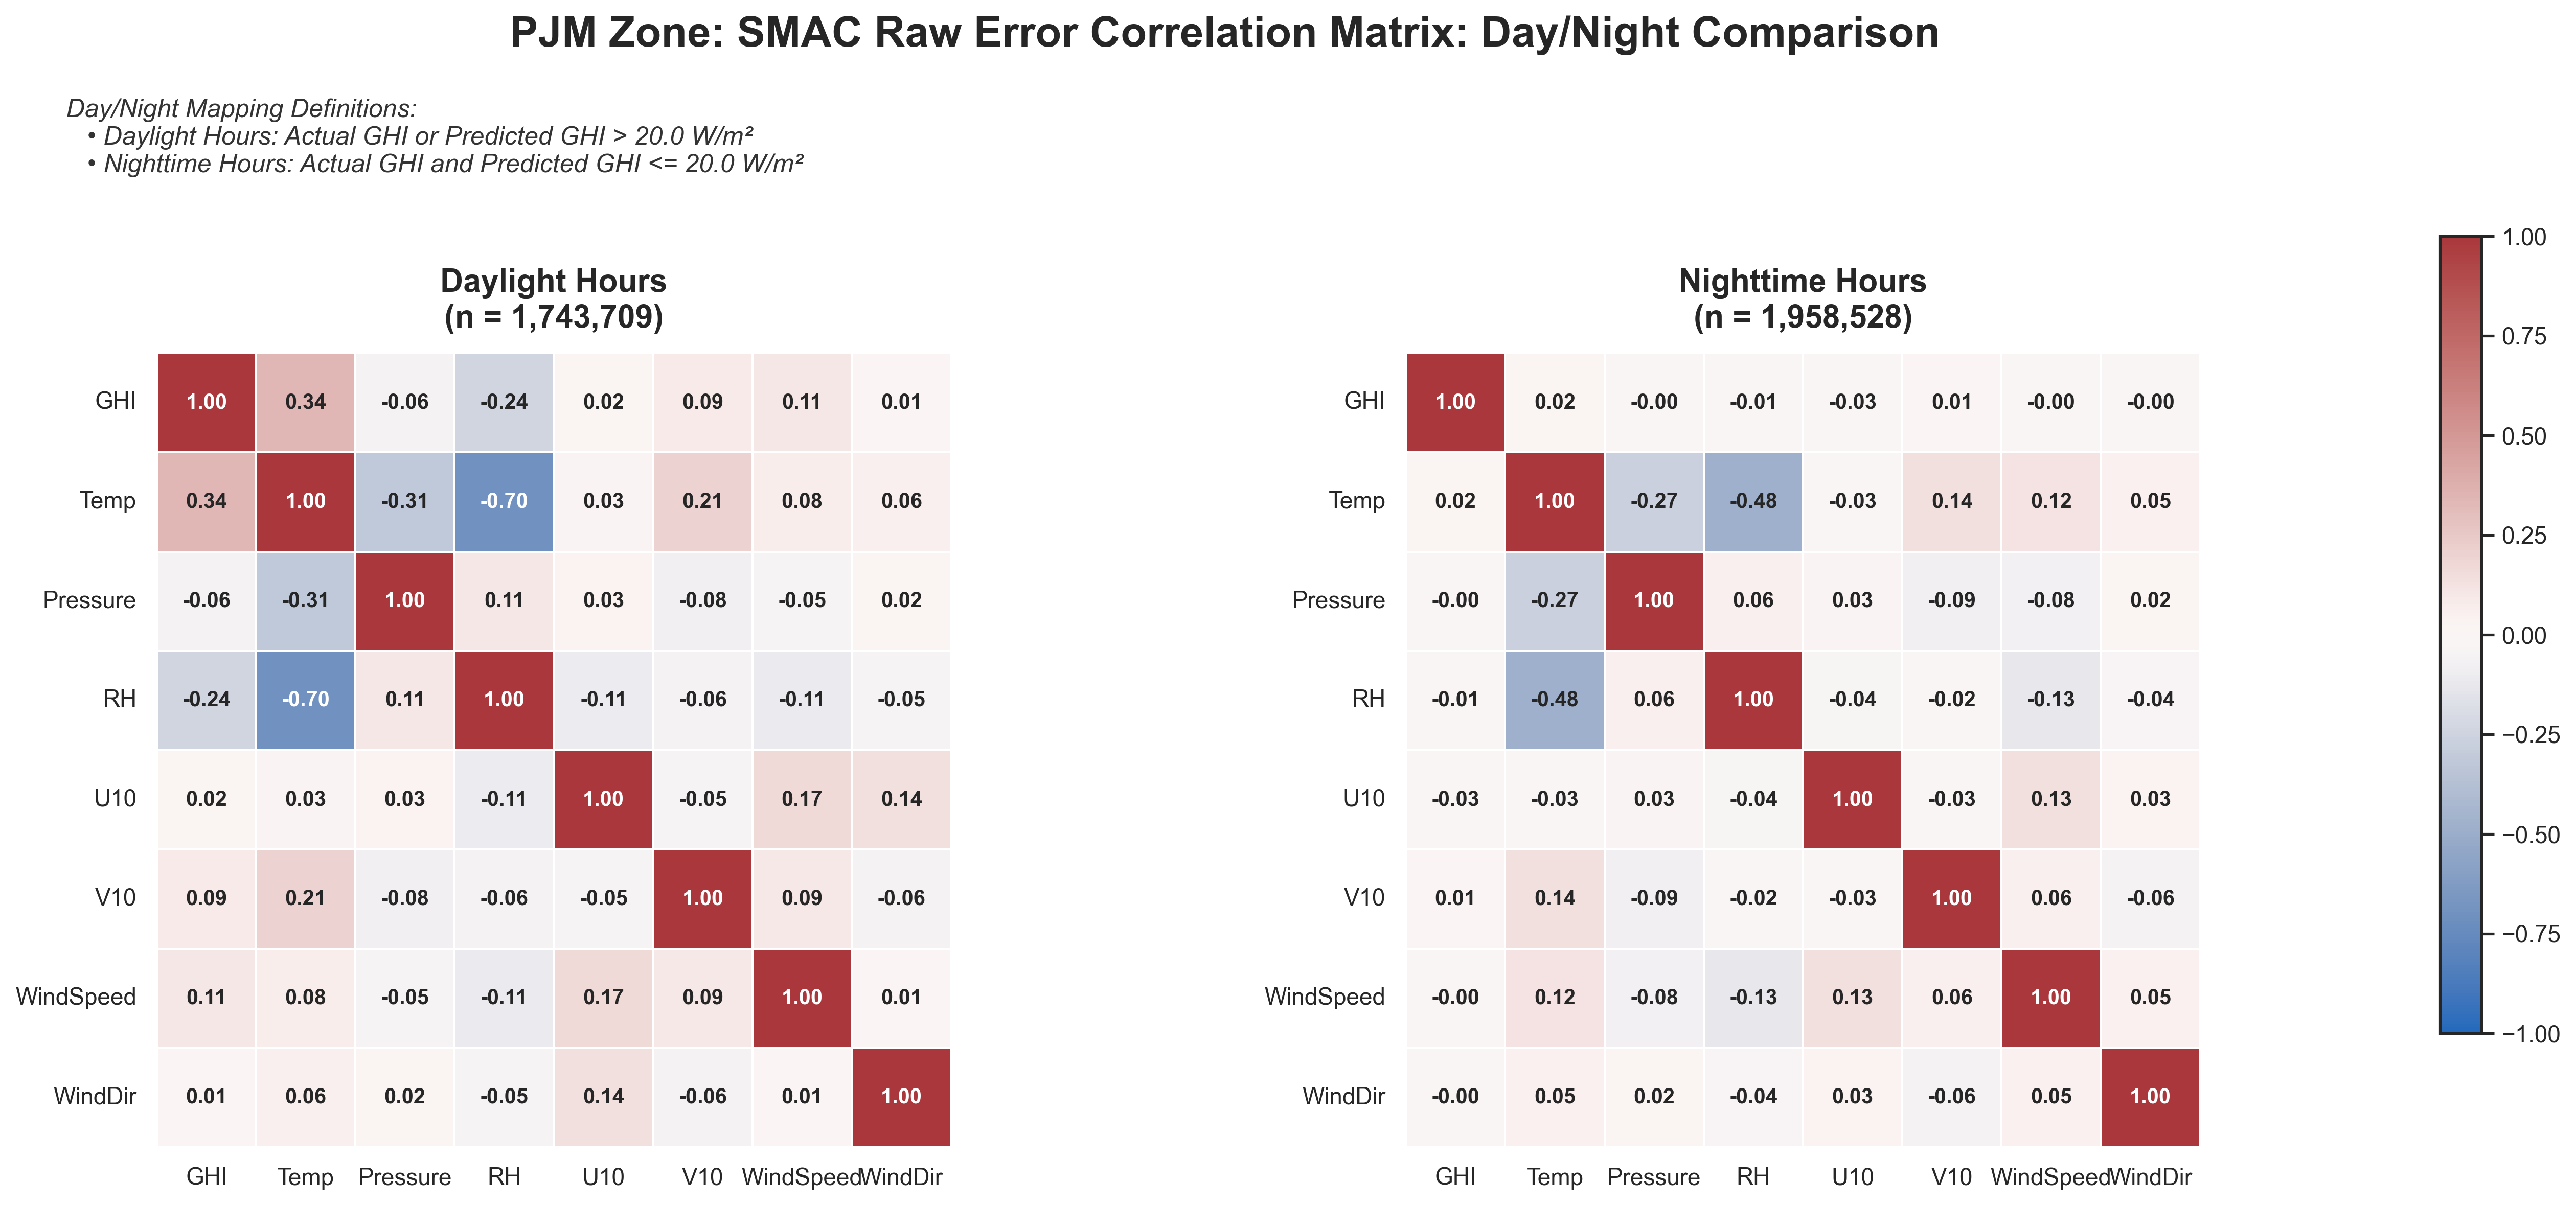
\includegraphics[width=\textwidth]{figures/Q7/ZONES/zone_corr_diurnal_split_smac.png}
  \caption{Cross-variable error matrices computed independently across major PJM transmission zones.}
  \label{fig:app_zone_smac}
\end{figure}

\begin{figure}[H]
  \centering
  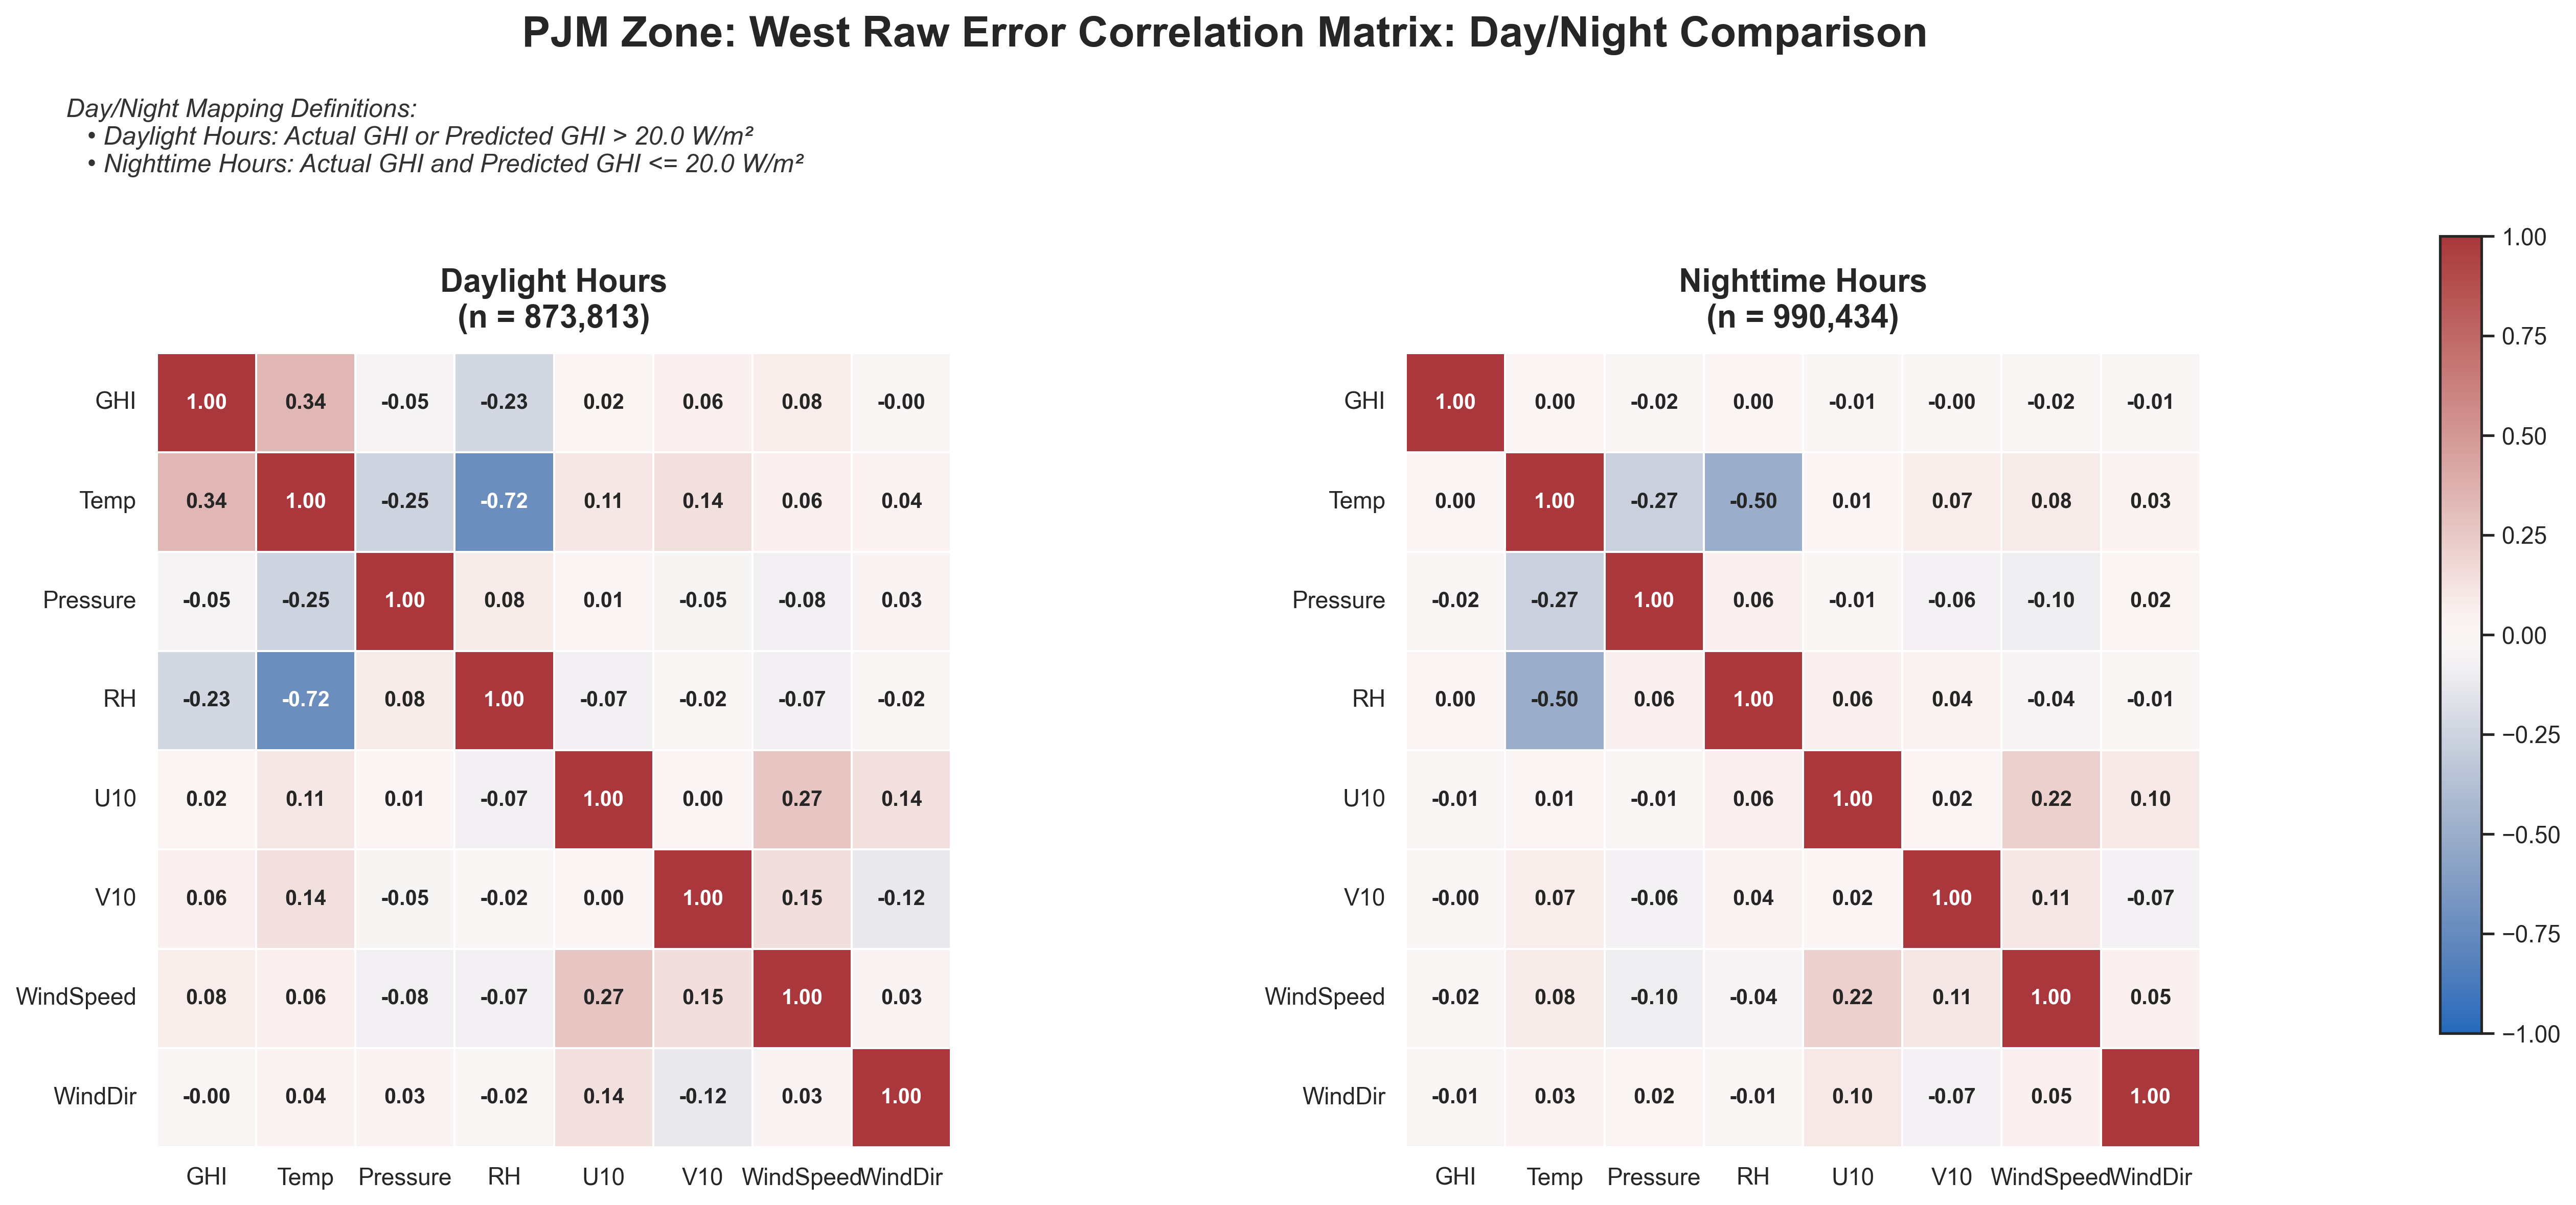
\includegraphics[width=\textwidth]{figures/Q7/ZONES/zone_corr_diurnal_split_west.png}
  \caption{Cross-variable error matrices computed independently across major PJM transmission zones.}
  \label{fig:app_zone_west}
\end{figure}

\begin{figure}[H]
  \centering
  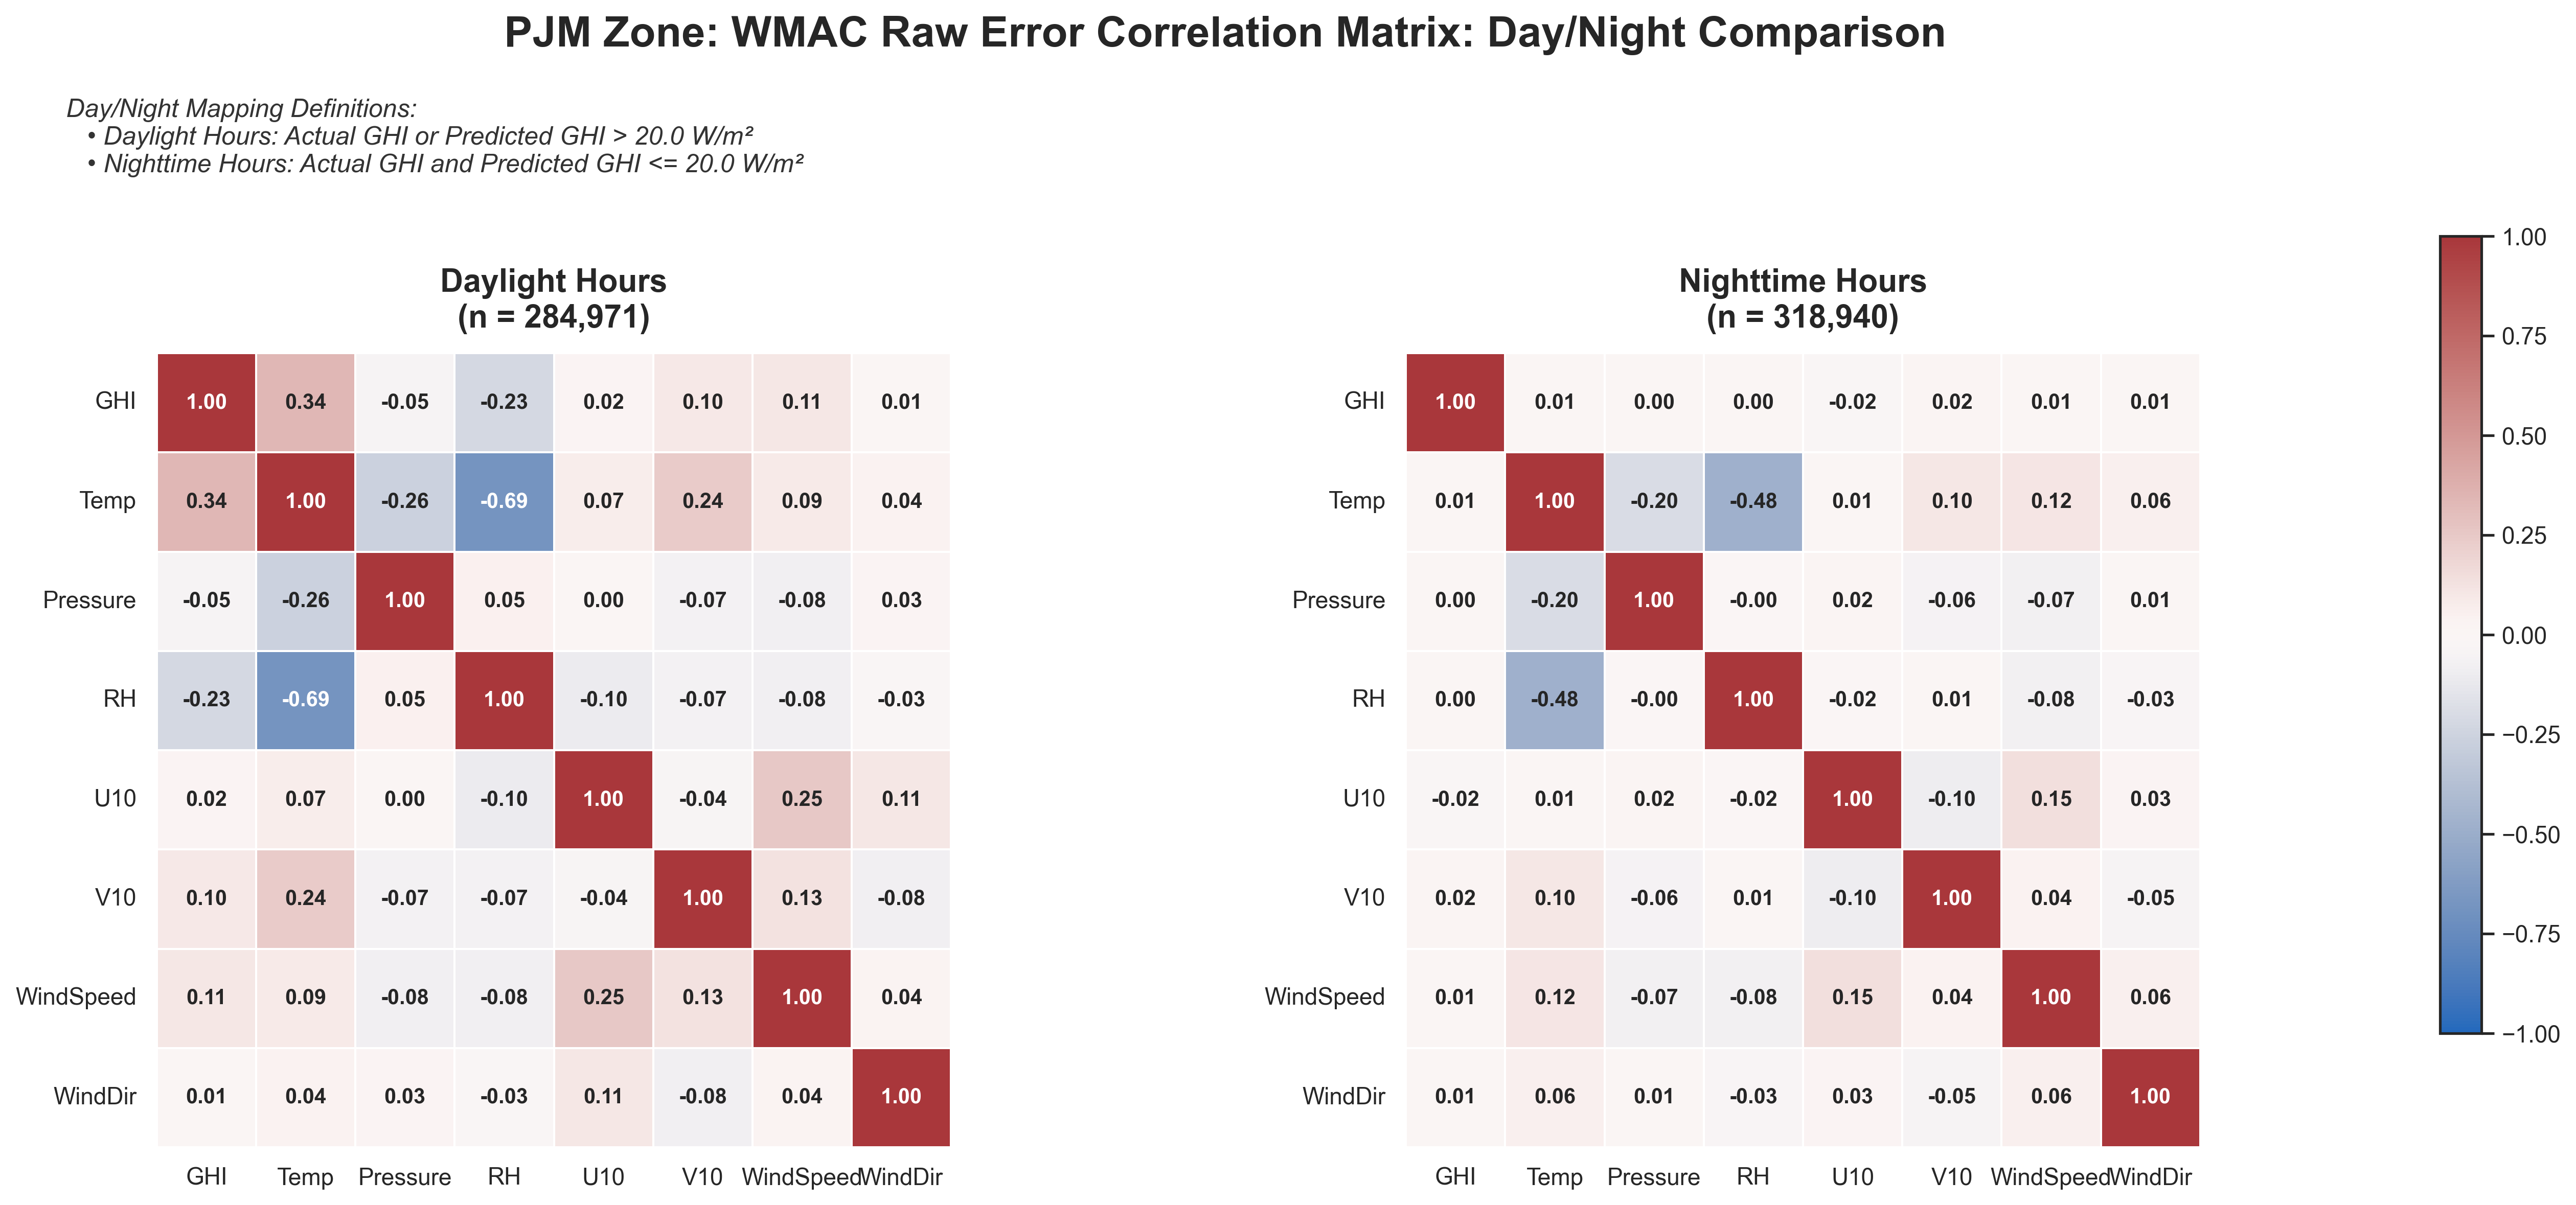
\includegraphics[width=\textwidth]{figures/Q7/ZONES/zone_corr_diurnal_split_wmac.png}
  \caption{Cross-variable error matrices computed independently across major PJM transmission zones.}
  \label{fig:app_zone_wmac}
\end{figure}


\subsection {Q8 — Spatial Correlation Across PJM Zones}

\begin{figure}[H]
  \centering
  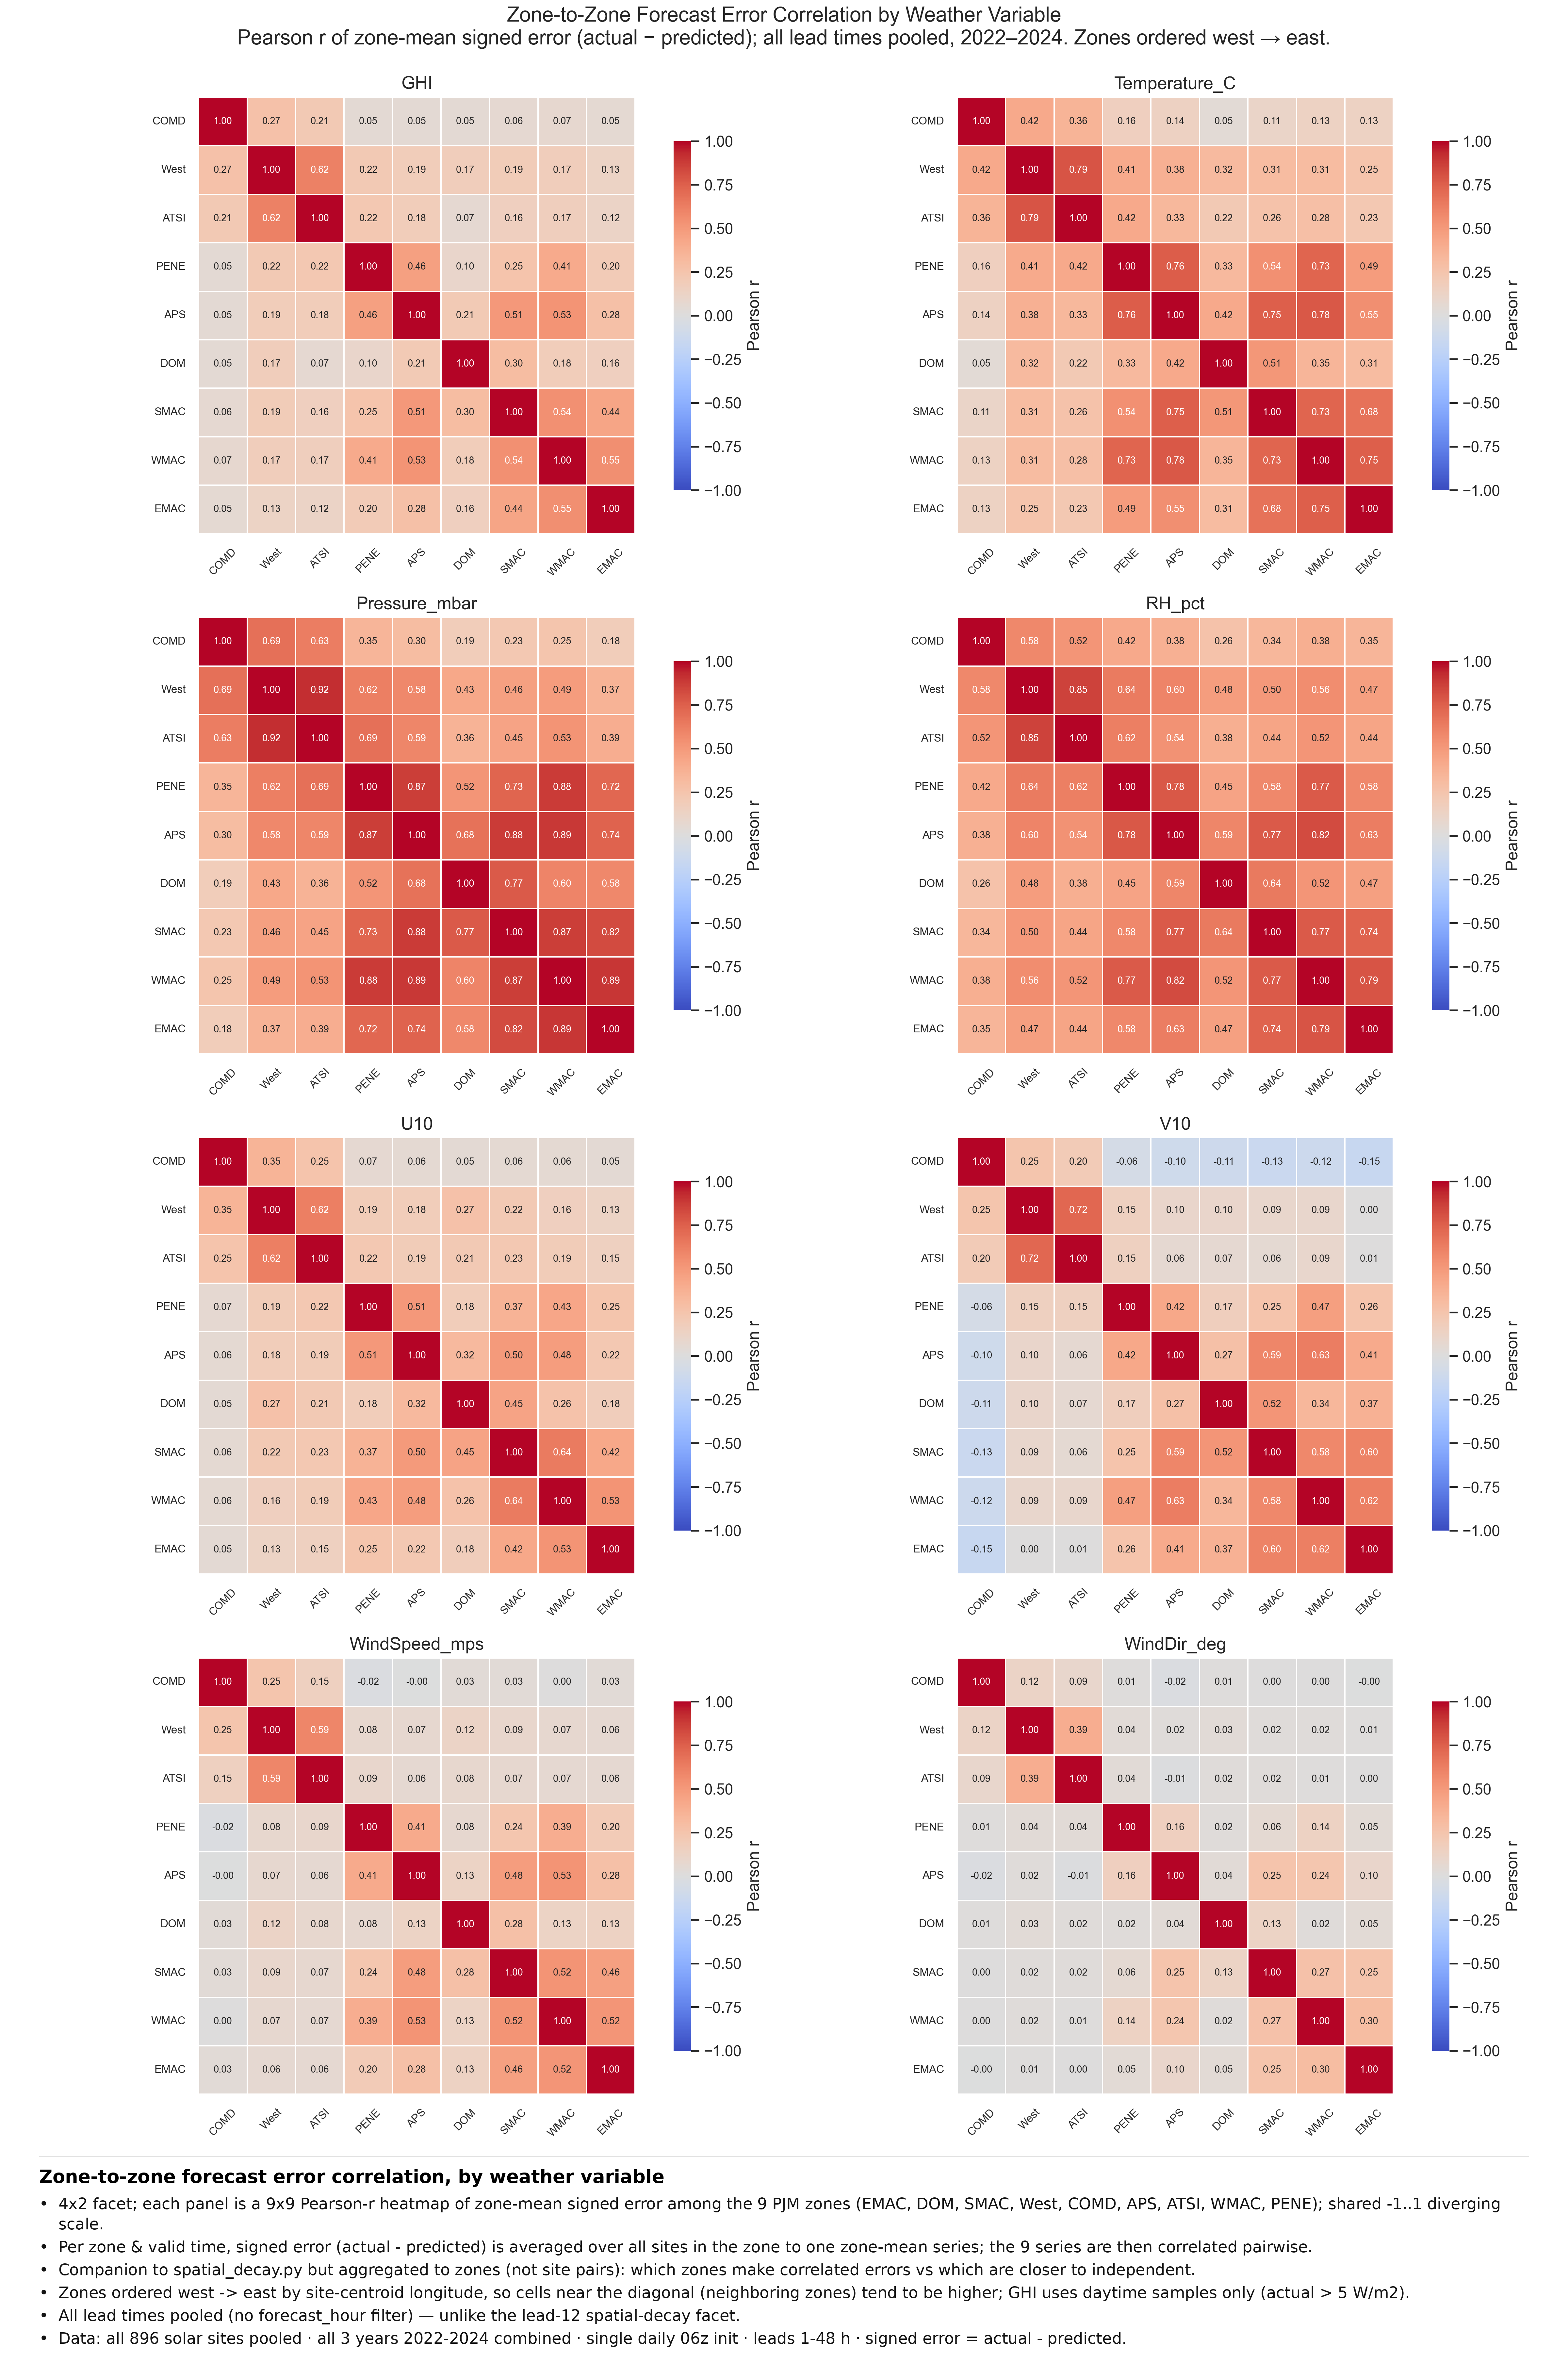
\includegraphics[width=\textwidth]{figures/Q8/zone_error_correlation.png}
  \caption{Complete (all-variable) version of the zone-to-zone forecast-error correlation matrices.}
  \label{fig:app_zonecorr}
\end{figure}

\begin{figure}[H]
  \centering
  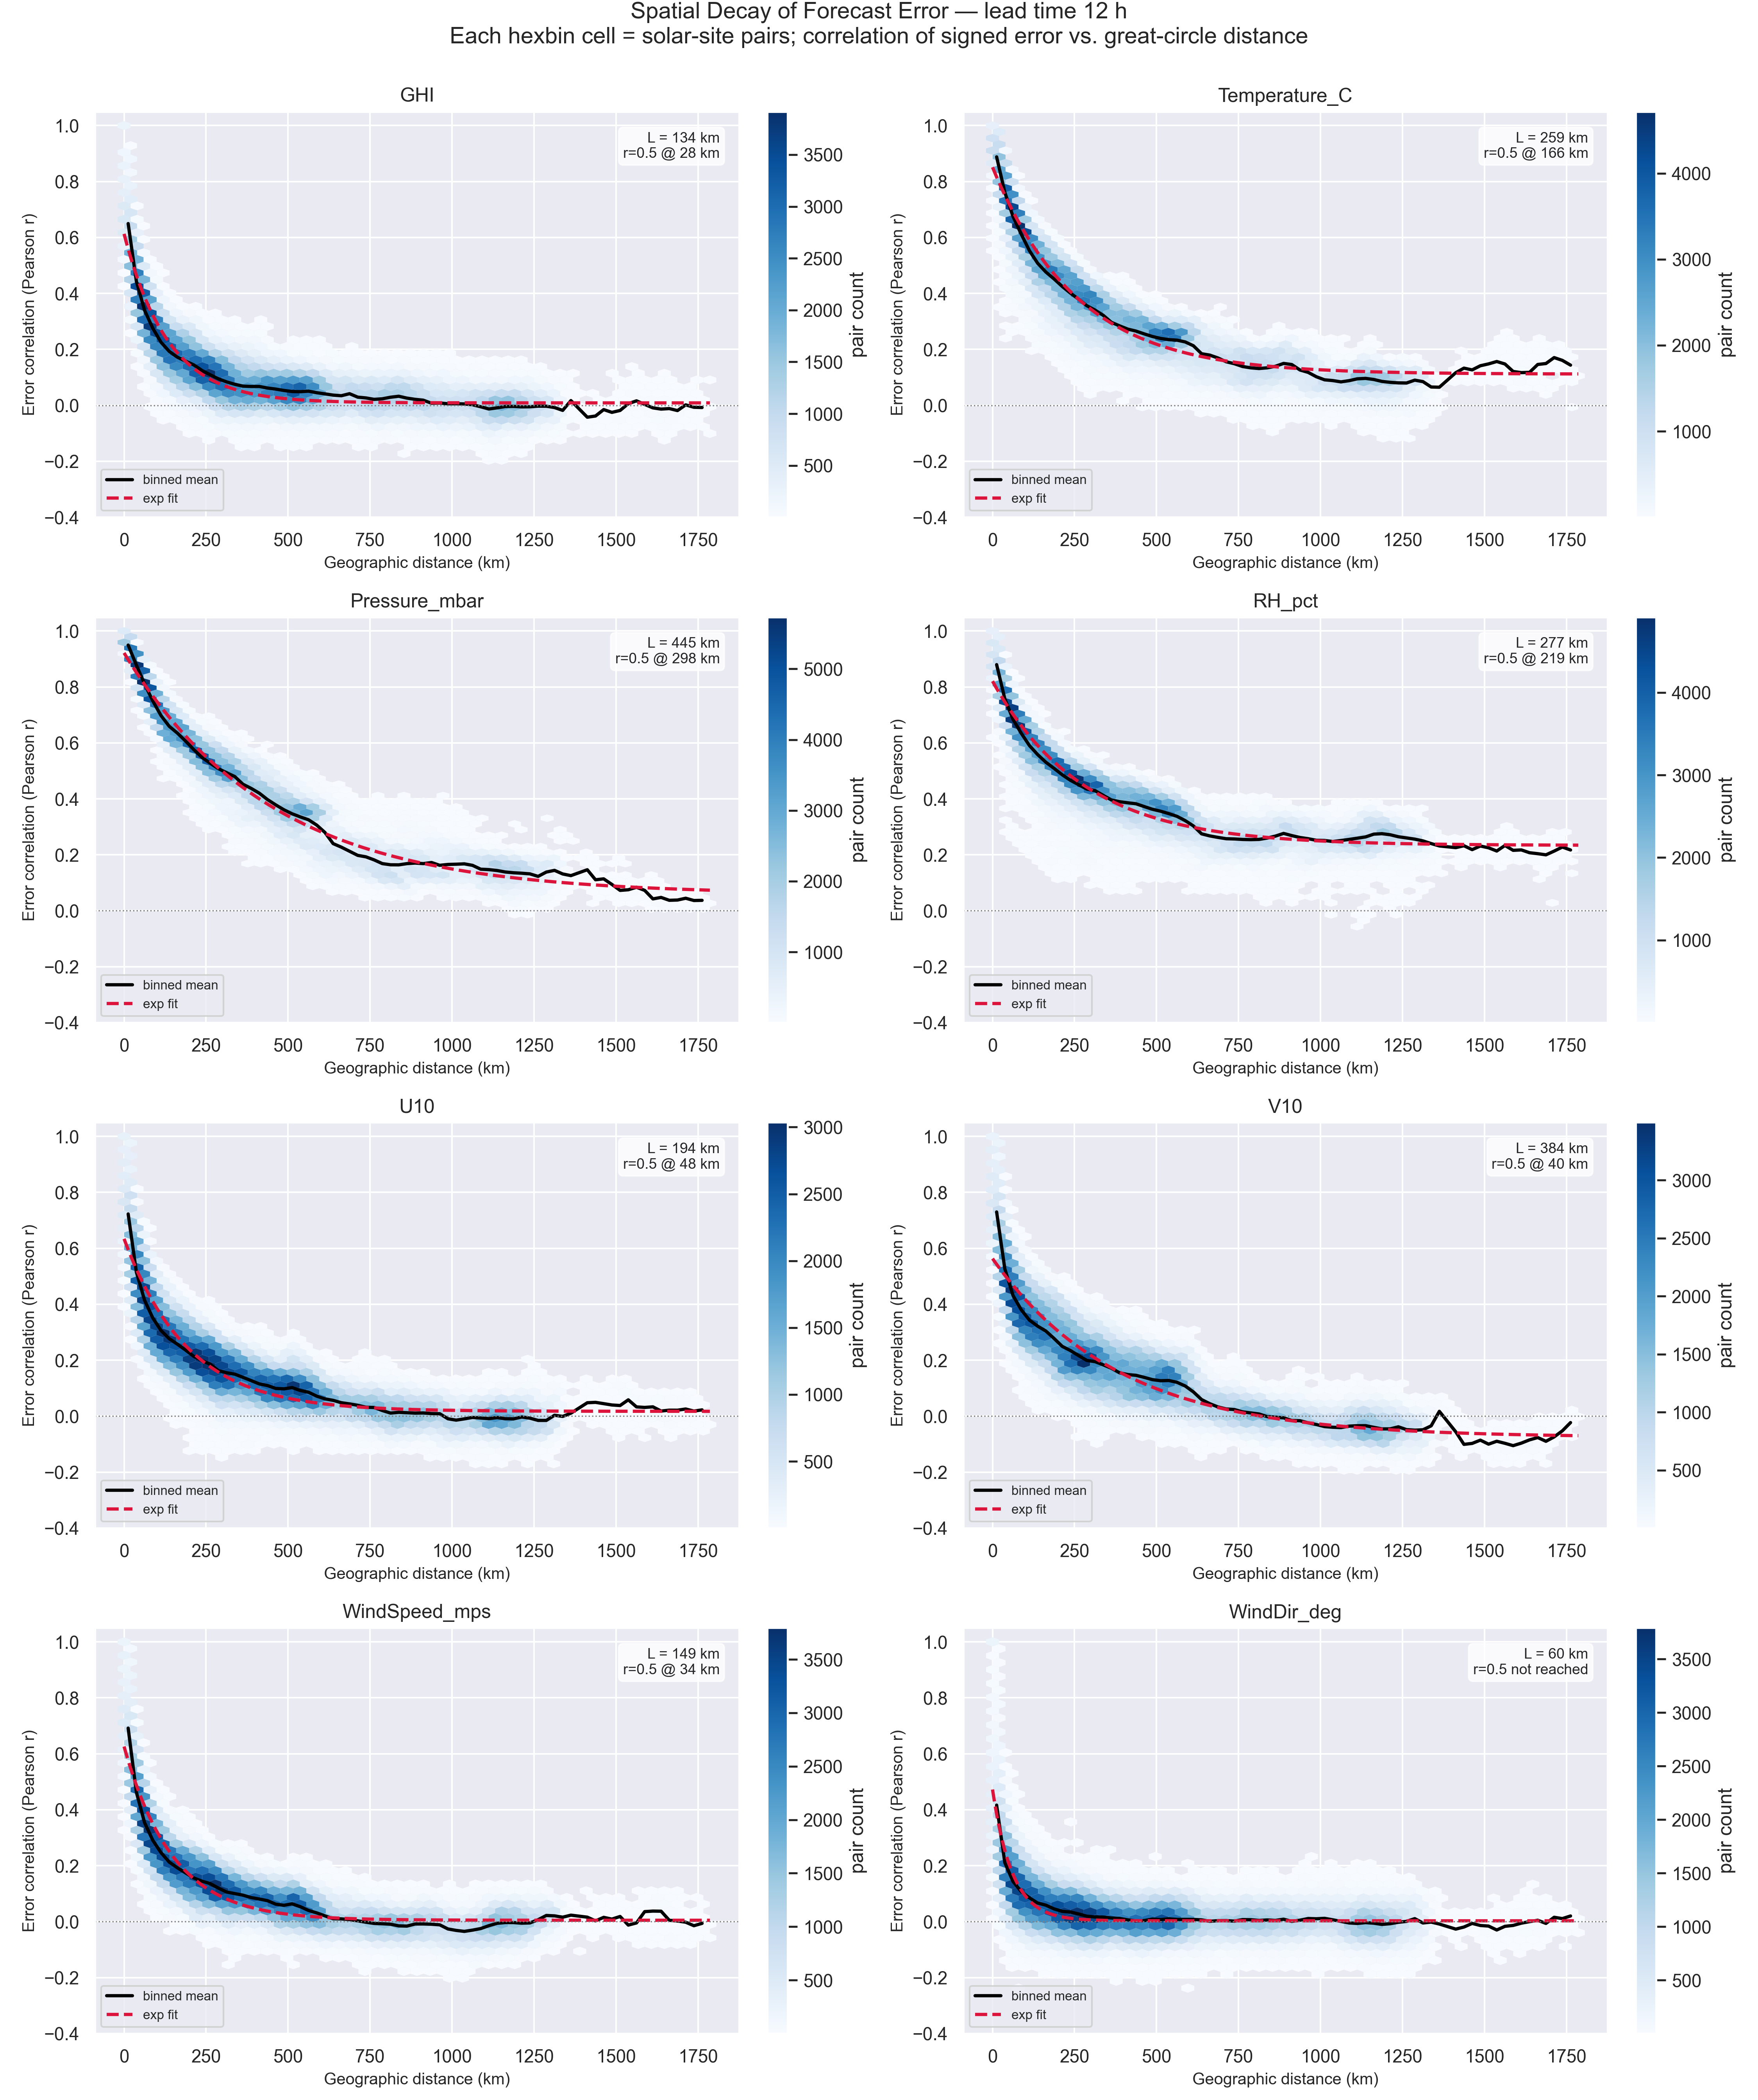
\includegraphics[width=\textwidth]{figures/Q8/spatial_decay_lead12.png}
  \caption{Spatial decay of forecast error at lead~12~h (= \texttt{18z}, solar noon). Each panel
  plots error correlation versus great-circle distance for all $\approx\num{400000}$ site pairs
  (hexbin density), with the distance-binned mean (black) and fitted exponential
  $\rho(d)=a\,e^{-d/L}+c$ (crimson). Pressure is the most spatially coherent
  ($L \approx \SI{445}{km}$); temperature ($L \approx \SI{233}{km}$) and RH
  ($L \approx \SI{277}{km}$) are intermediate; GHI decorrelates fastest
  ($L \approx \SI{134}{km}$, $r=0.5$ by $\sim\SI{28}{km}$); wind direction is so noisy its fit
  never reaches $r=0.5$.}
  \label{fig:decay12}
\end{figure}

Sweeping the lead time (Figure~\ref{fig:decaylead}) shows how both the \emph{reach} ($L$) and the
\emph{strength} of correlation evolve.

\begin{figure}[H]
  \centering
  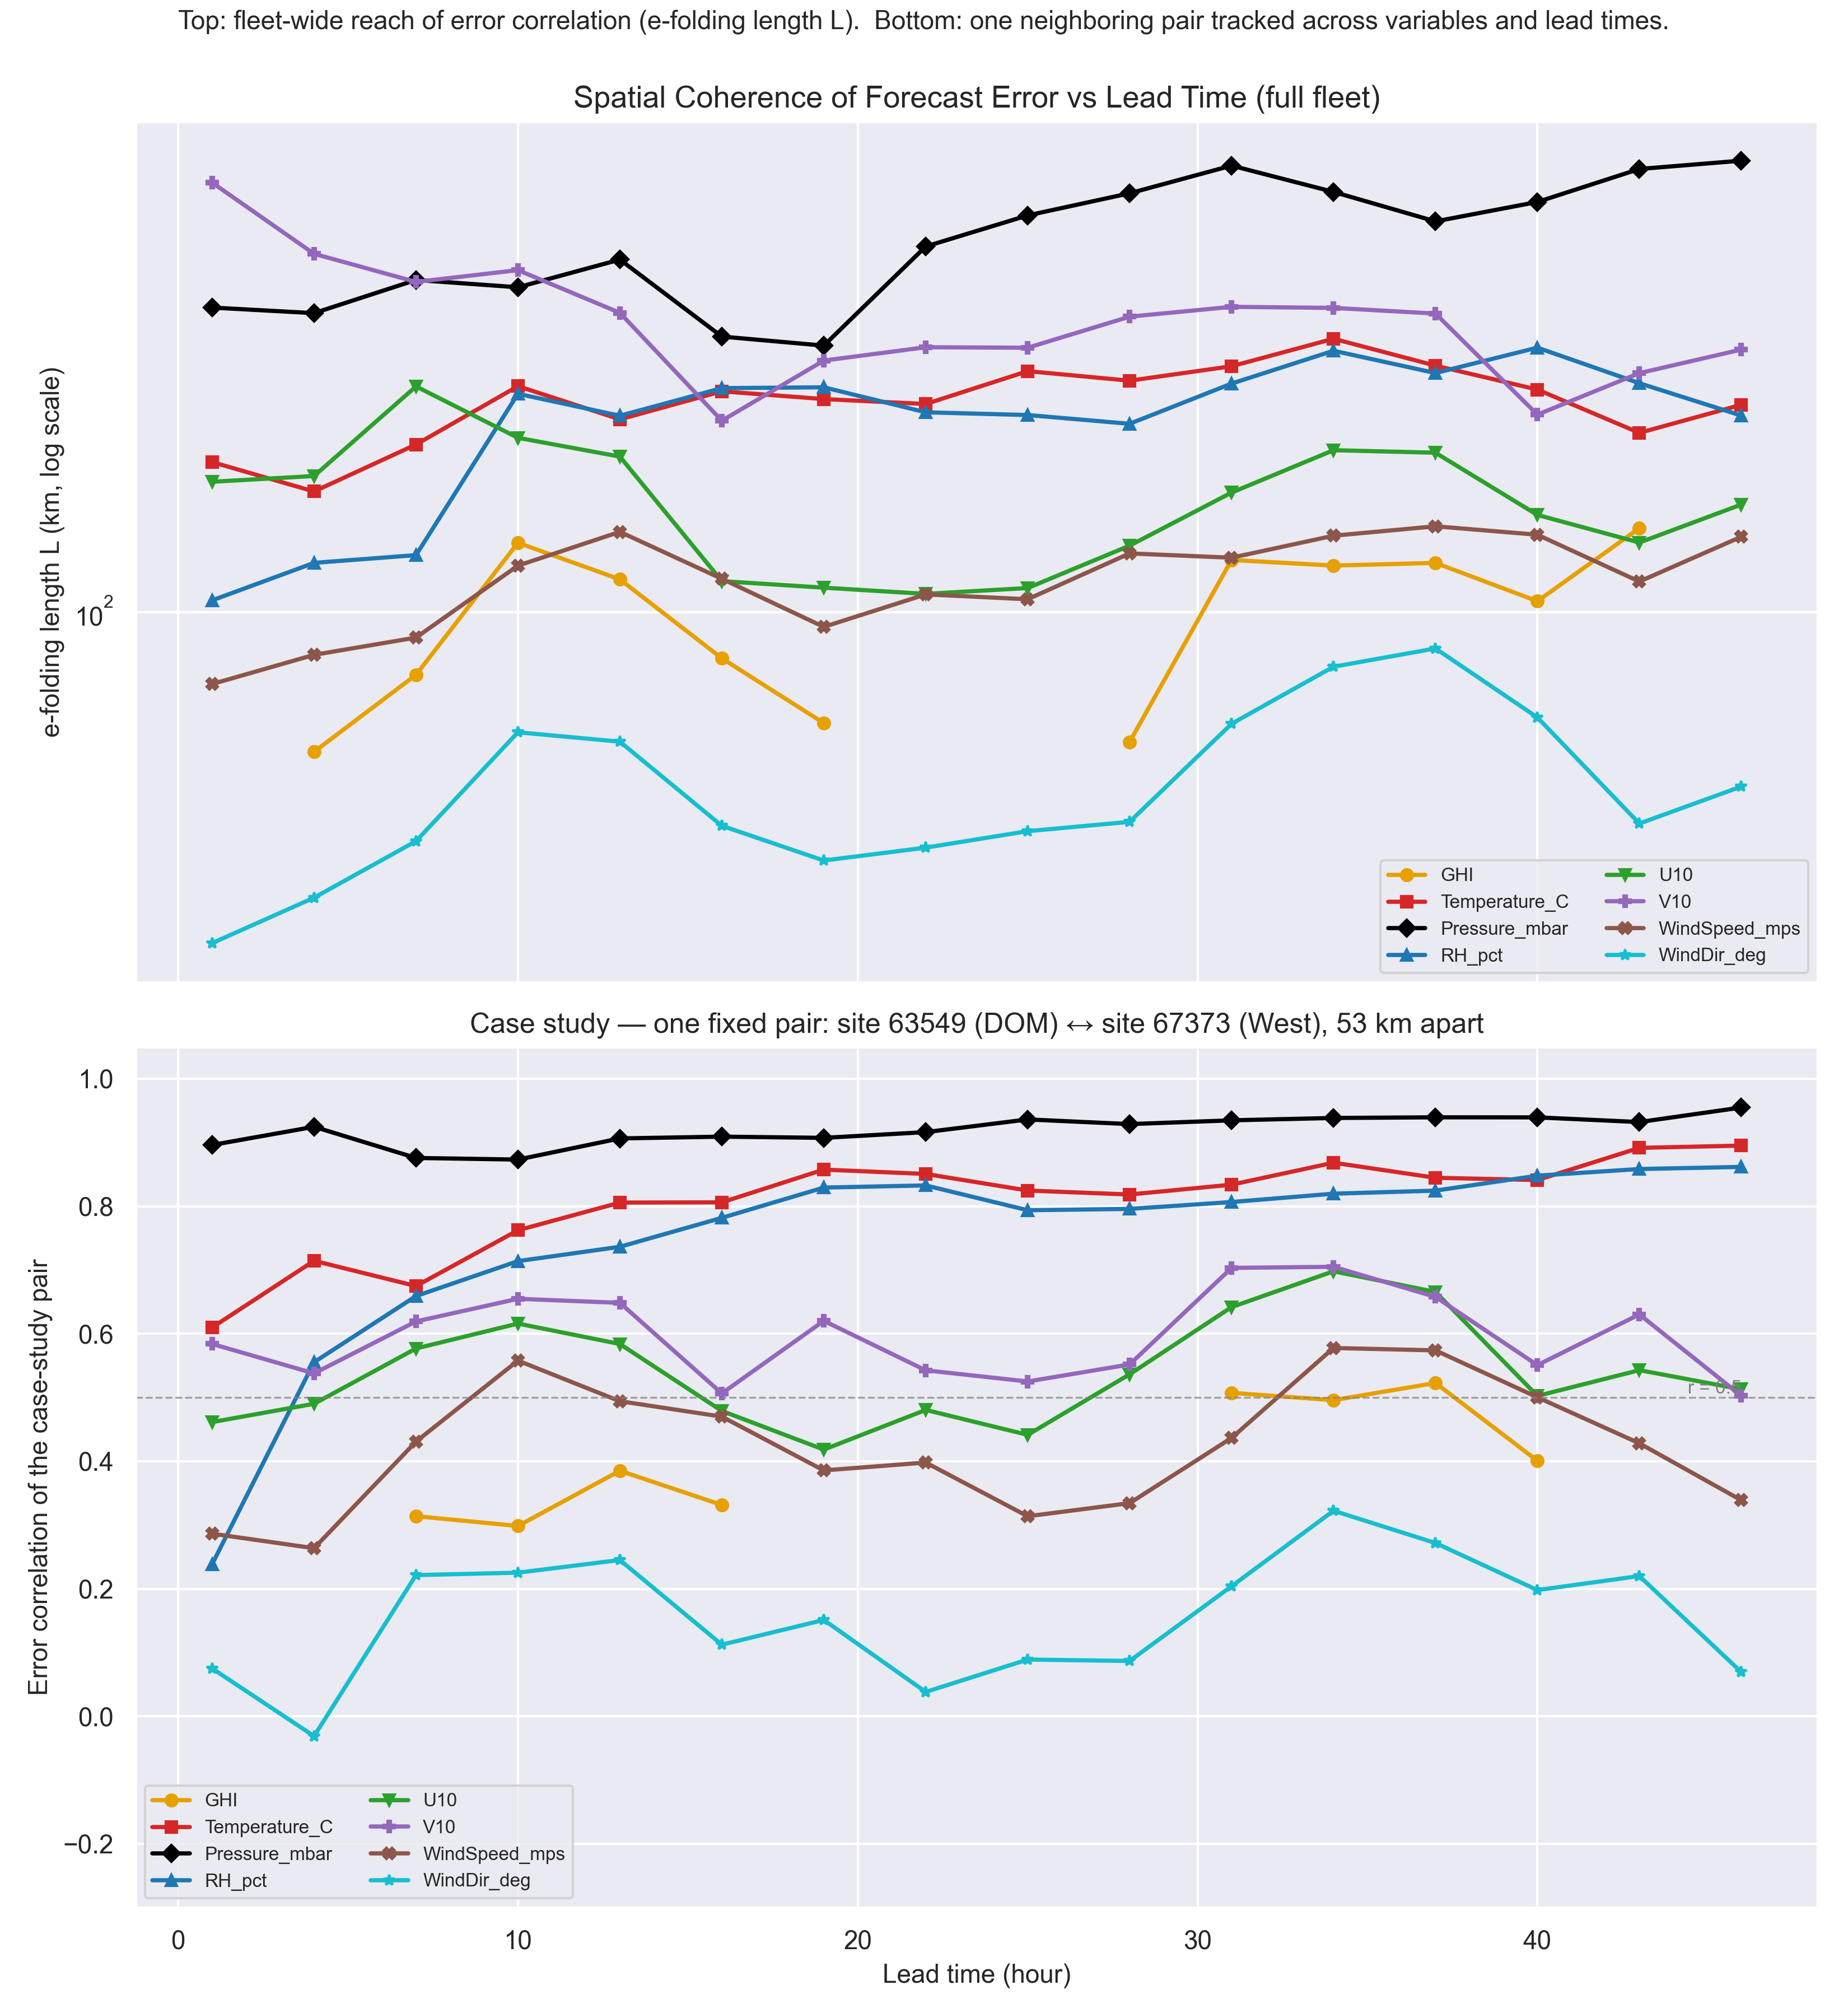
\includegraphics[width=\textwidth]{figures/Q8/decorrelation_length_by_lead_time.png}
  \caption{Spatial coherence versus lead time. \emph{Top:} fitted e-folding length $L$ (log
  scale) for the full fleet---$L$ generally grows with lead time for the synoptic variables
  (pressure reaches farthest; RH and temperature rise), consistent with errors becoming
  larger-scale further out, while wind direction has the shortest $L$ at every lead.
  \emph{Bottom:} a case study tracking one fixed neighbouring pair (site 63549, DOM
  $\leftrightarrow$ site 67373, West; \SI{53}{km} apart) across variables and leads, which
  reproduces the fleet ranking in miniature. Note (Section~\ref{sec:confound}) the lead axis also
  sweeps time of day, so GHI only has daytime-UTC points.}
  \label{fig:decaylead}
\end{figure}

\subsection{Q9 — Spatial Correlation Variation by Stratum}

\begin{figure}[H]
  \centering
  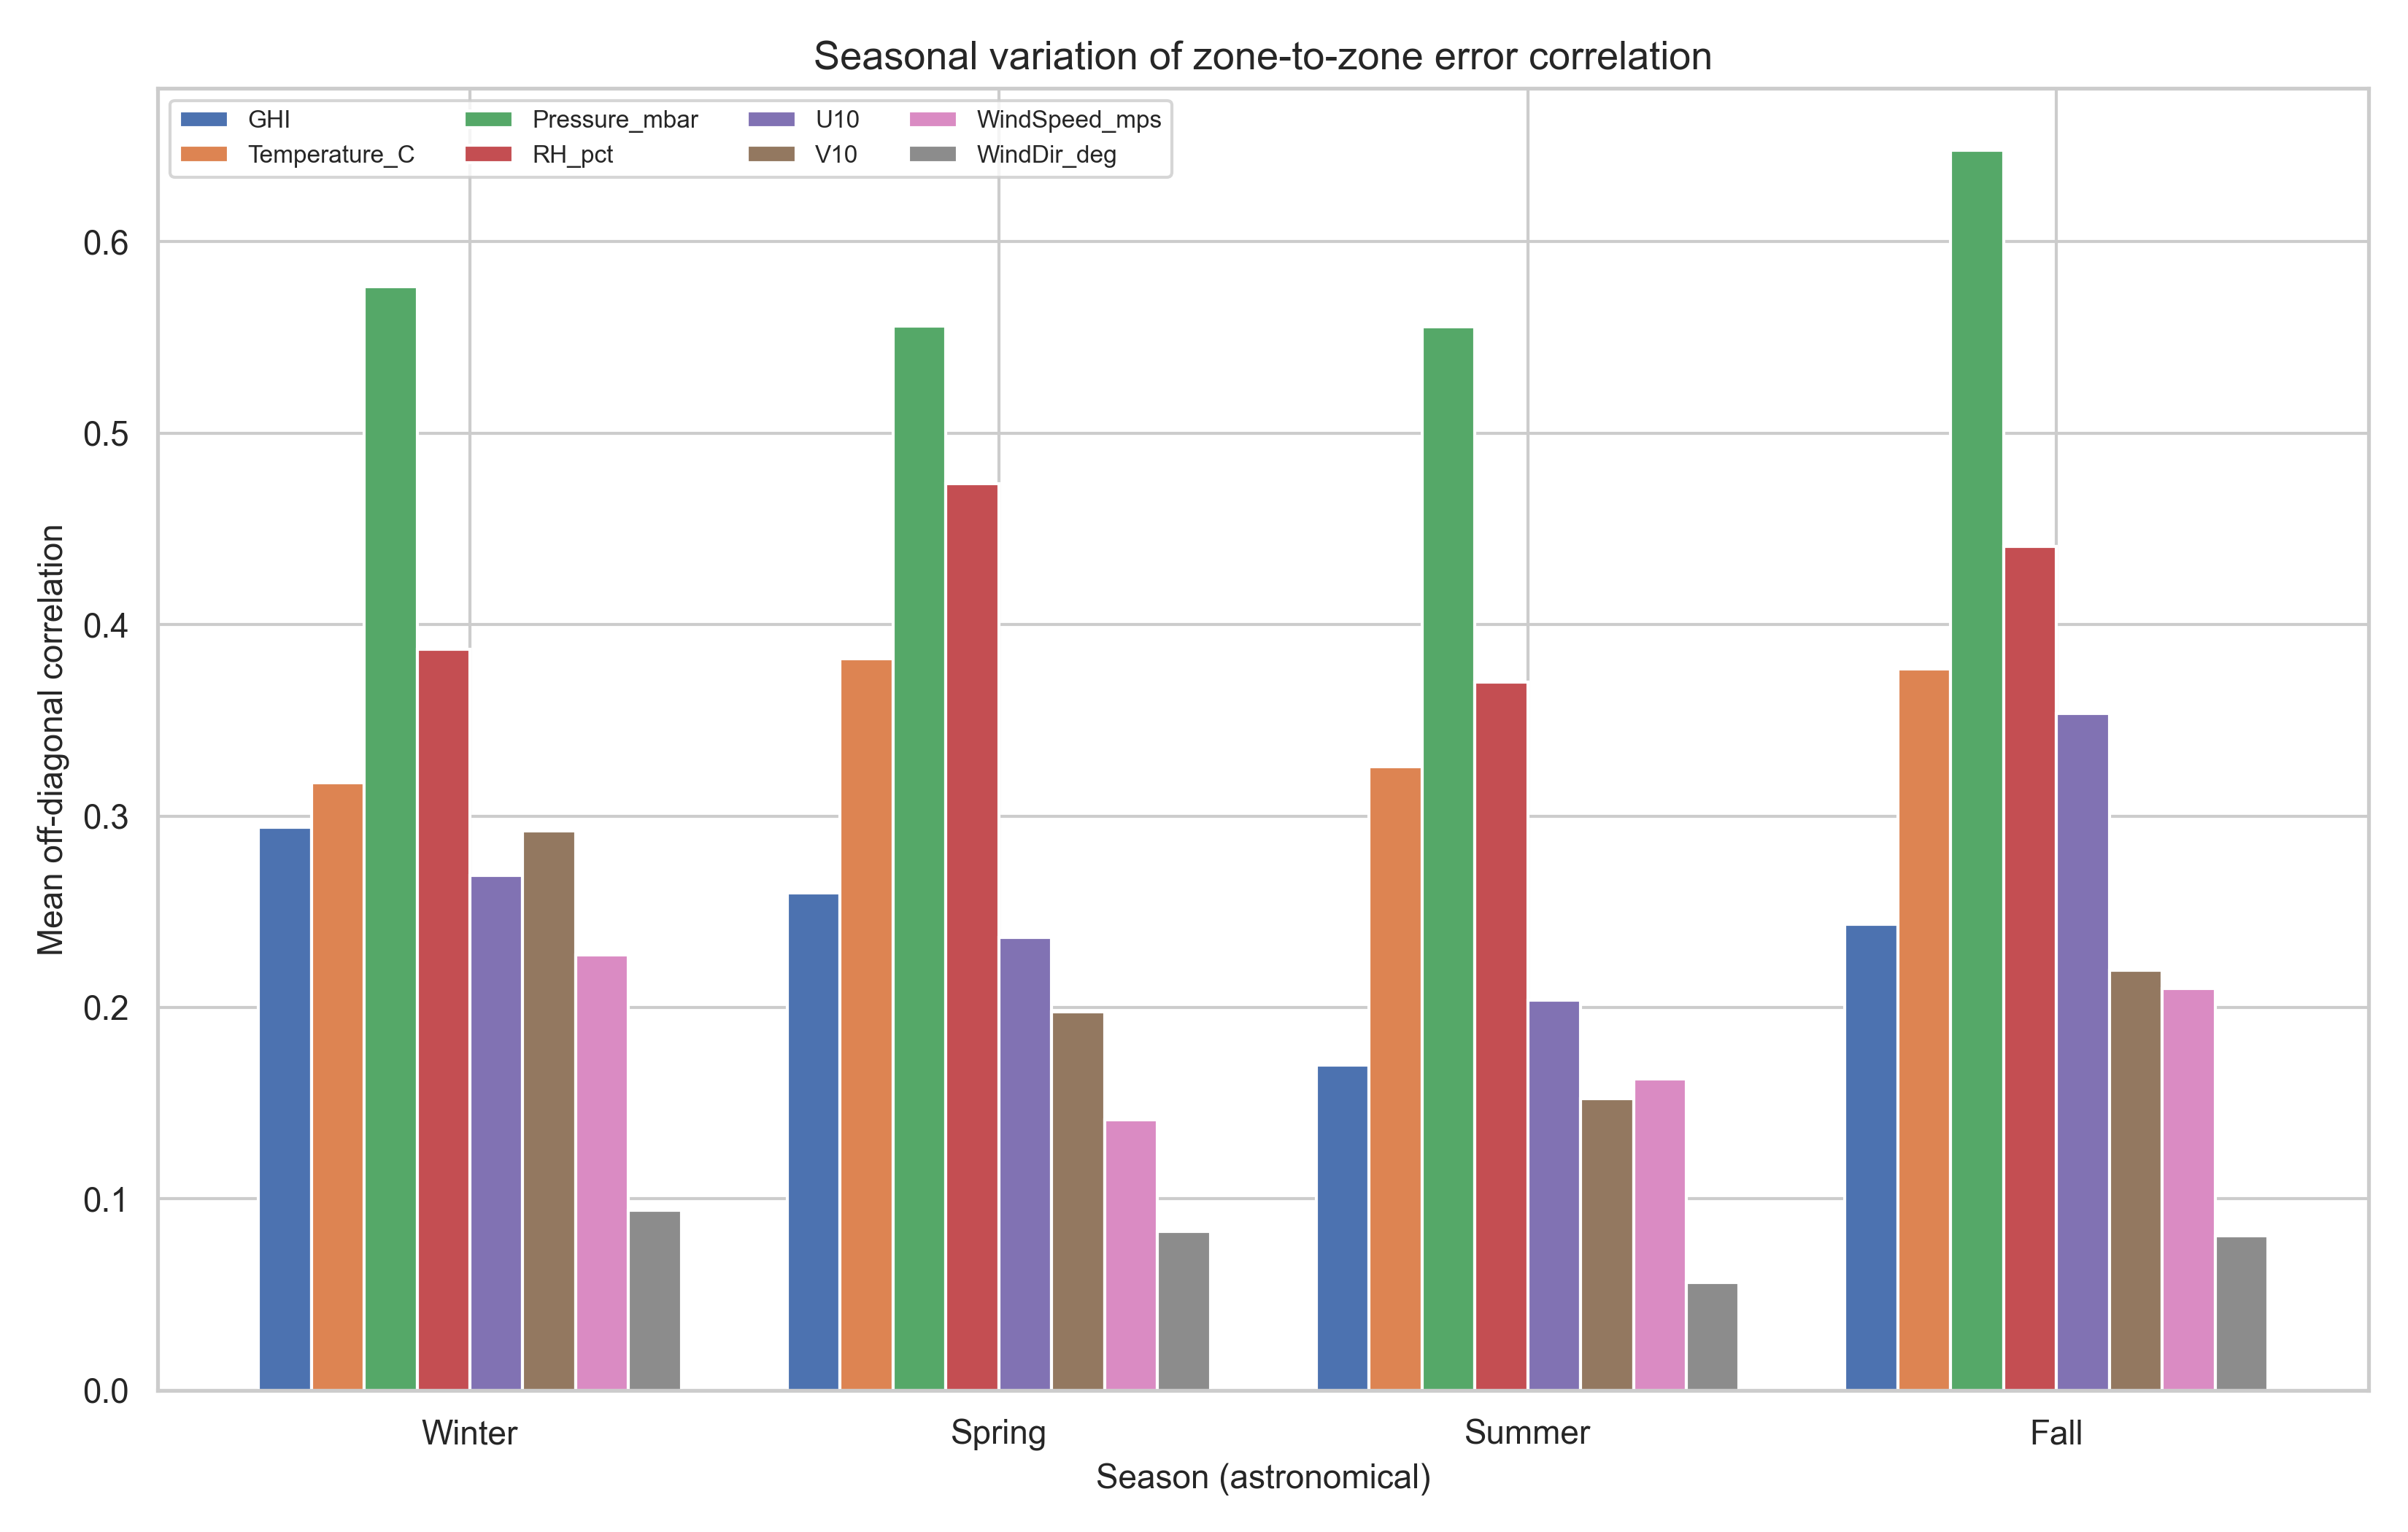
\includegraphics[width=\textwidth]{figures/Q9/seasonal_zone_correlation.png}
  \caption{Complete (all-variable) version of mean zone-to-zone correlation by season.}
  \label{fig:app_seasoncorr}
\end{figure}

\begin{figure}[H]
  \centering
  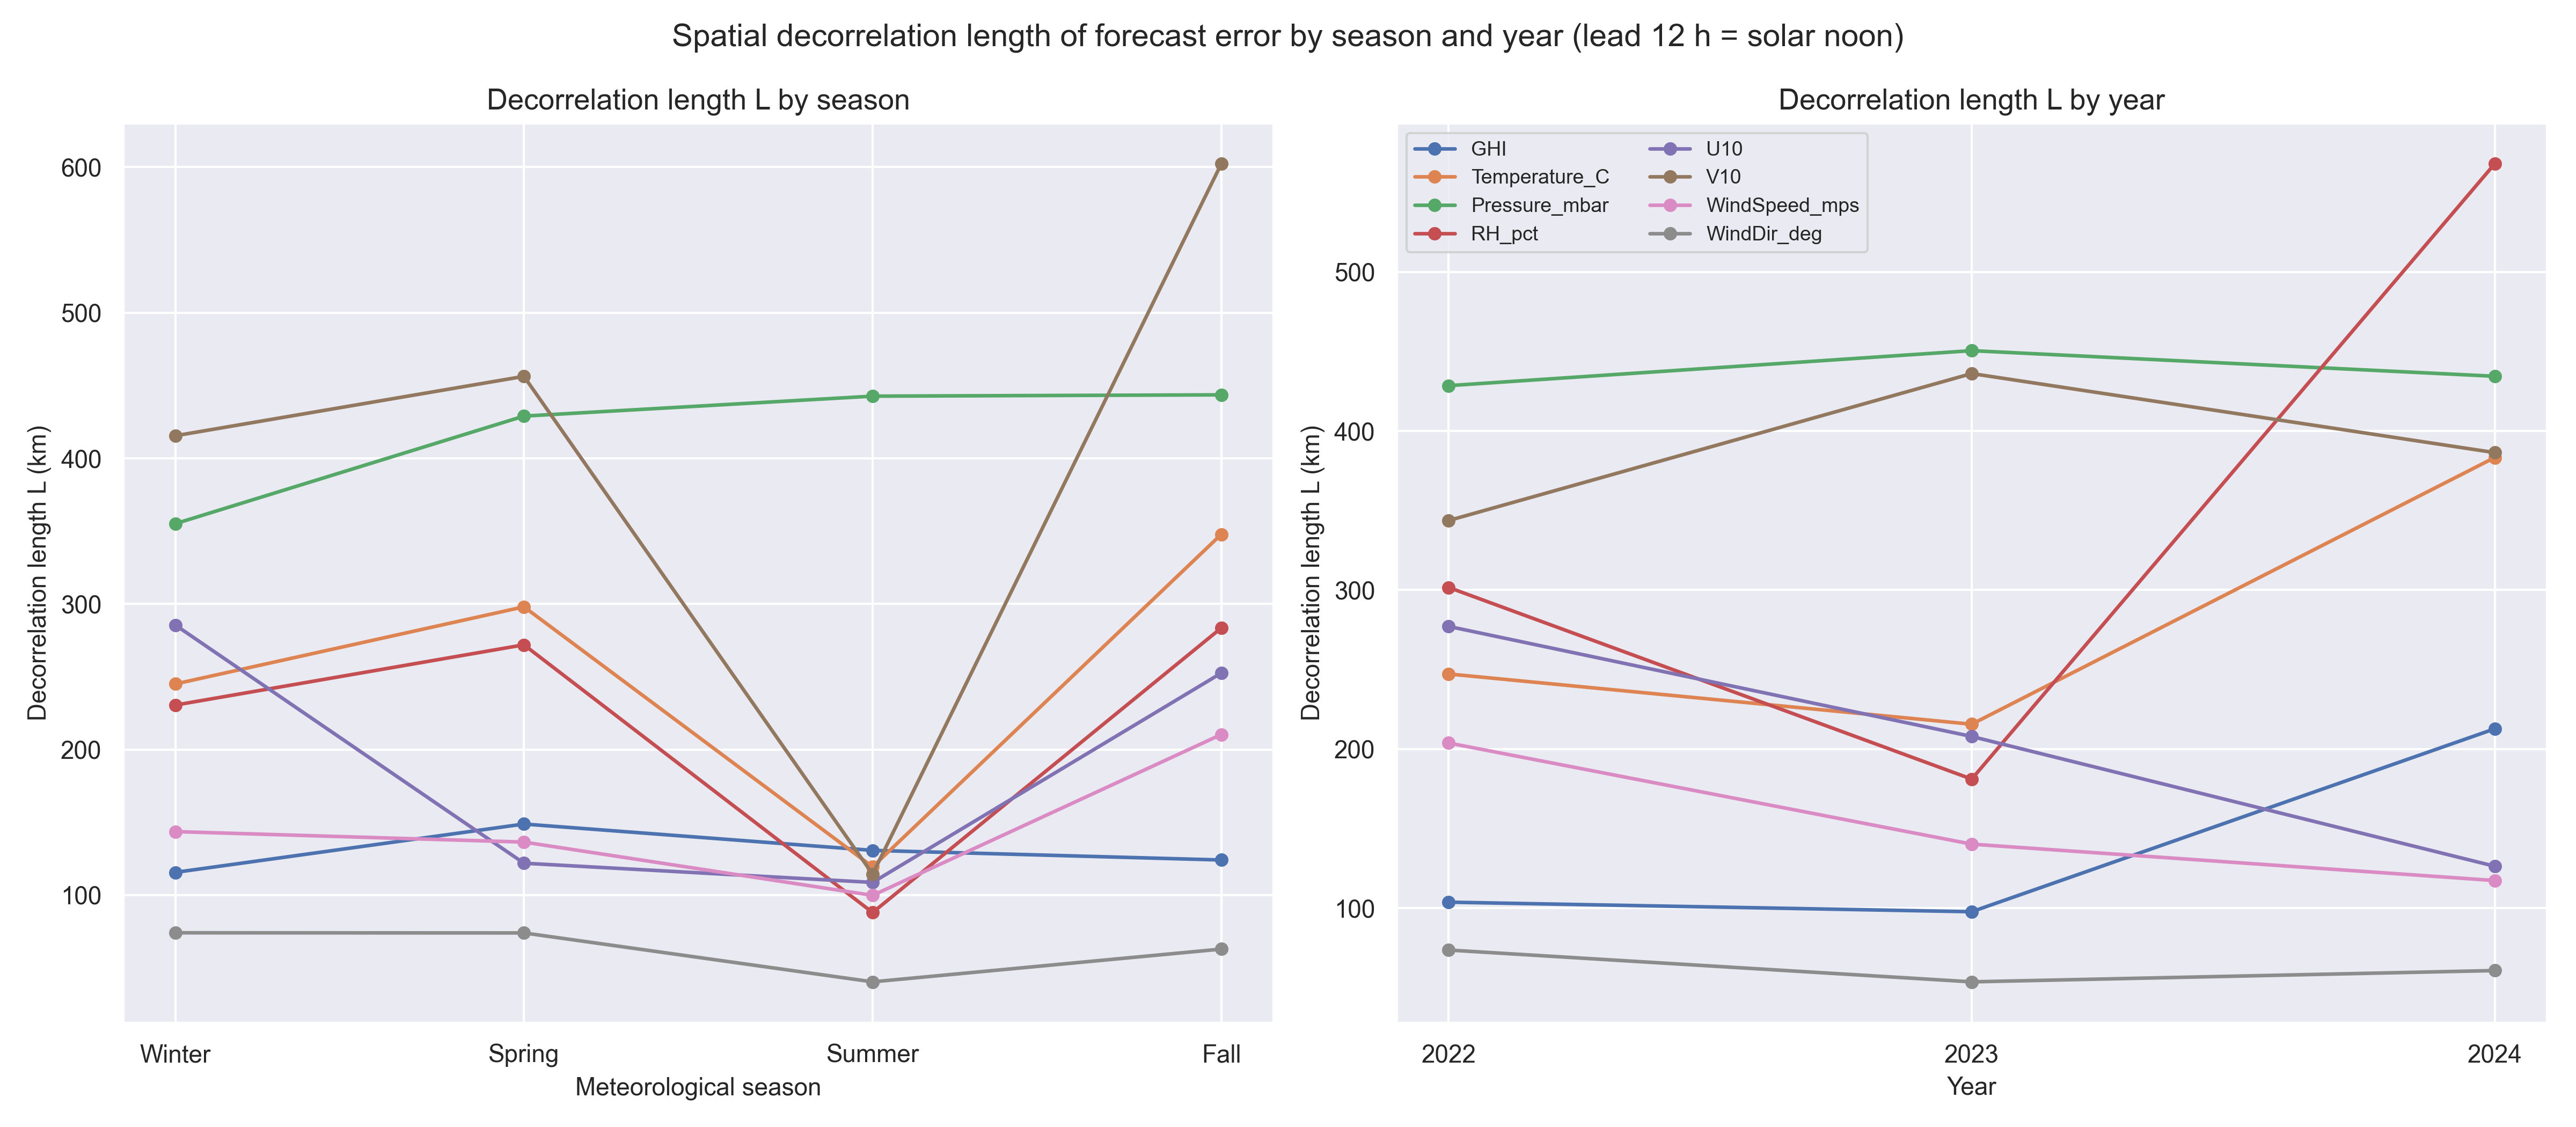
\includegraphics[width=\textwidth]{figures/Q9/decorrelation_length_by_season_year.png}
  \caption{Complete (all-variable) version of the fitted decorrelation length $L$ by season and year.}
  \label{fig:app_seasondecay}
\end{figure}

\begin{figure}[H]
  \centering
  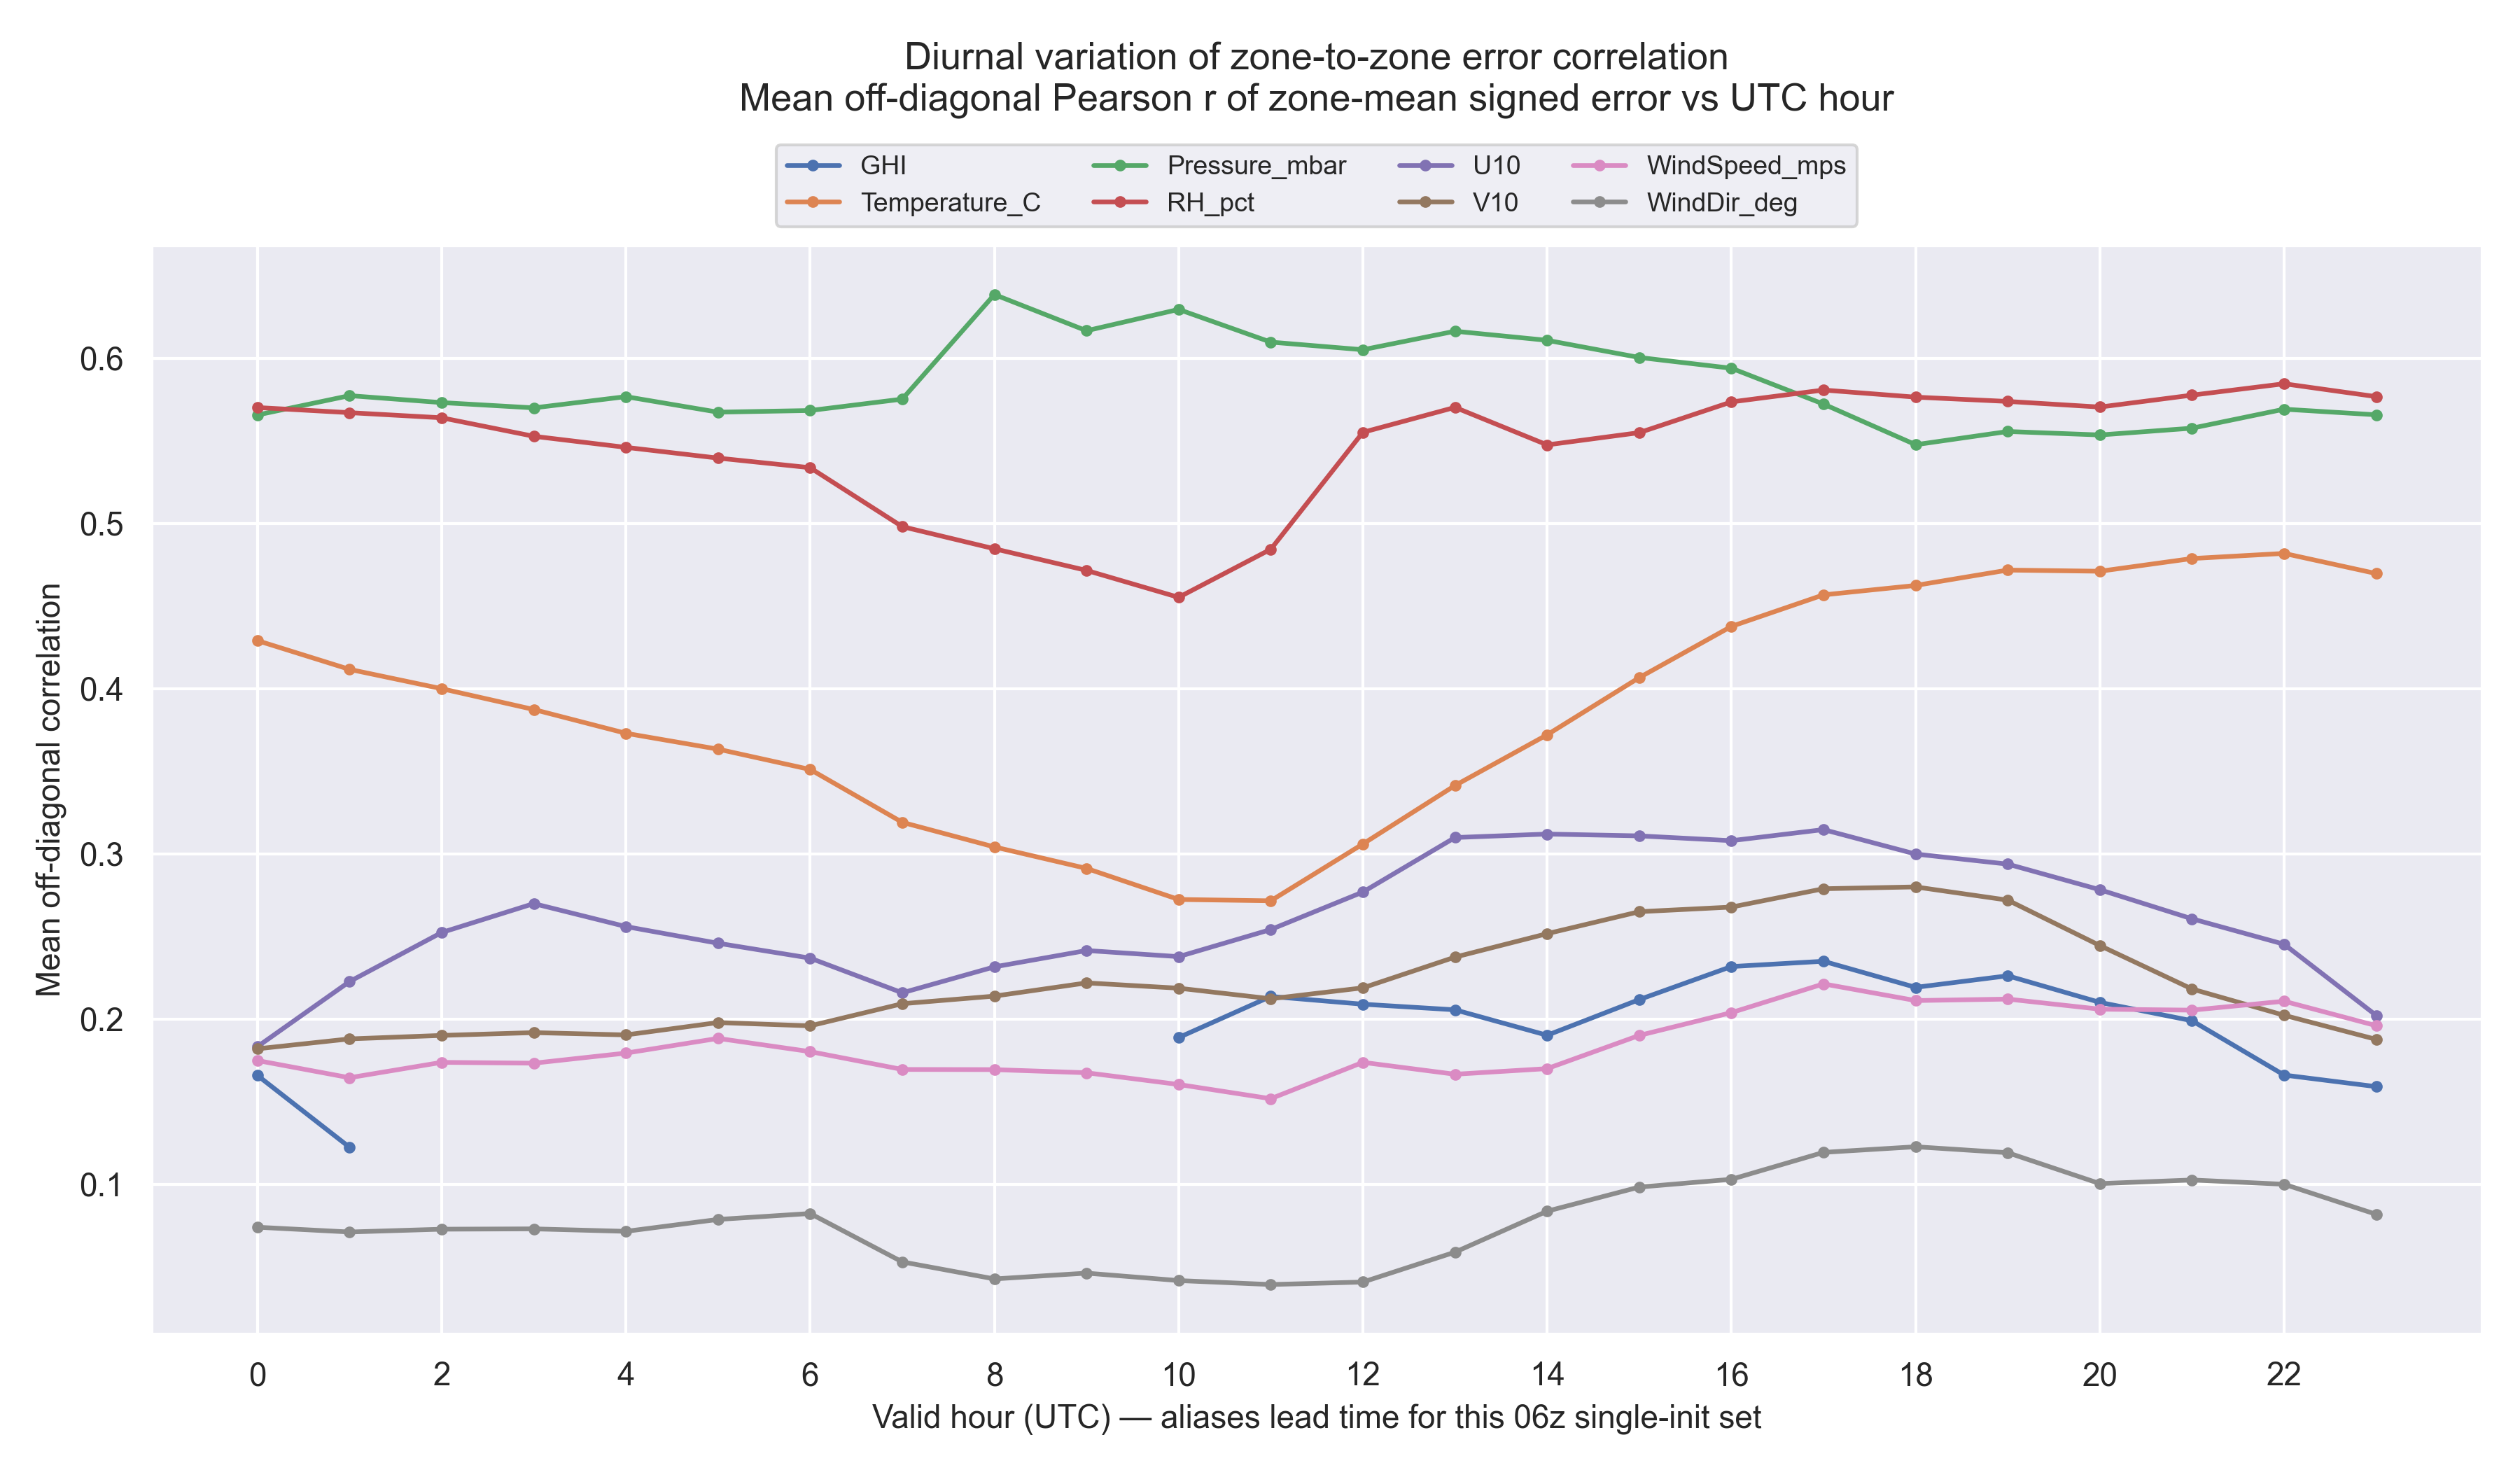
\includegraphics[width=\textwidth]{figures/Q9/diurnal_zone_correlation.png}
  \caption{Complete (all-variable) version of mean zone-to-zone correlation versus UTC hour.}
  \label{fig:app_diurnal}
\end{figure}

\begin{figure}[H]
  \centering
  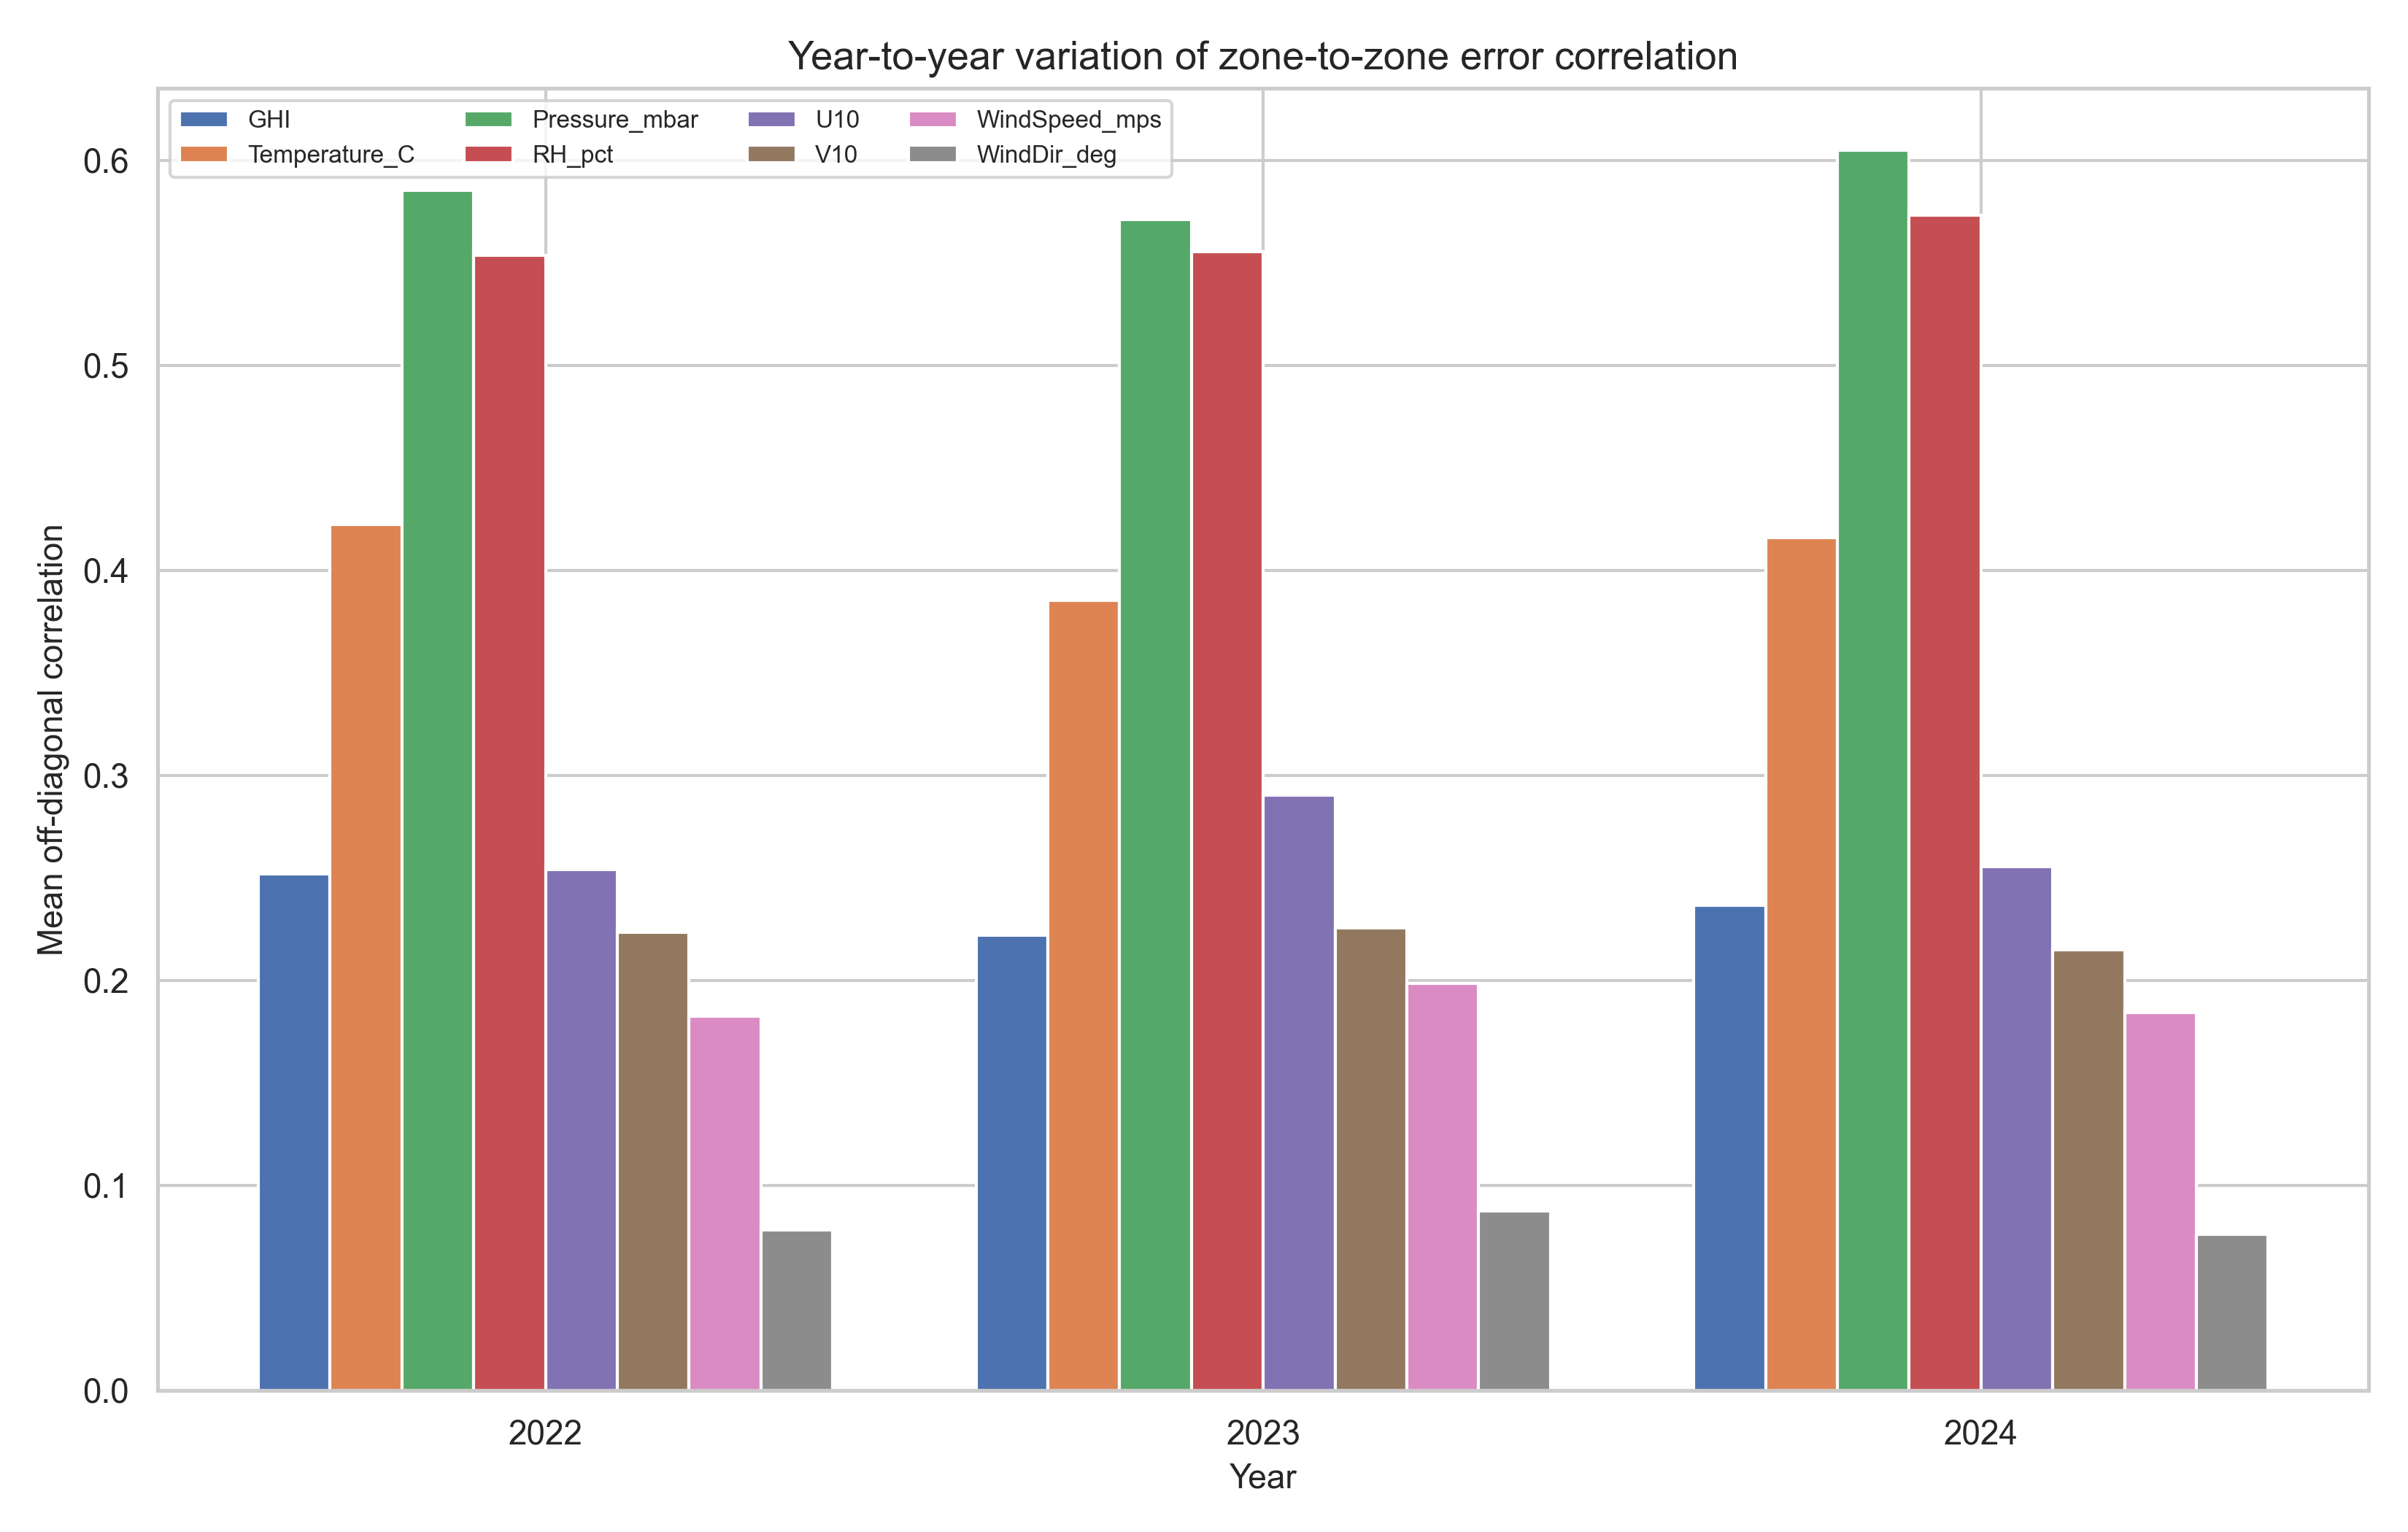
\includegraphics[width=\textwidth]{figures/Q9/yearly_zone_correlation.png}
  \caption{Complete (all-variable) version of year-to-year zone-to-zone forecast-error correlation.}
  \label{fig:app_yearcorr}
\end{figure}

\subsection{Q11 — Threshold-Sensitivity Sweep}

\begin{figure}[H]
  \centering
  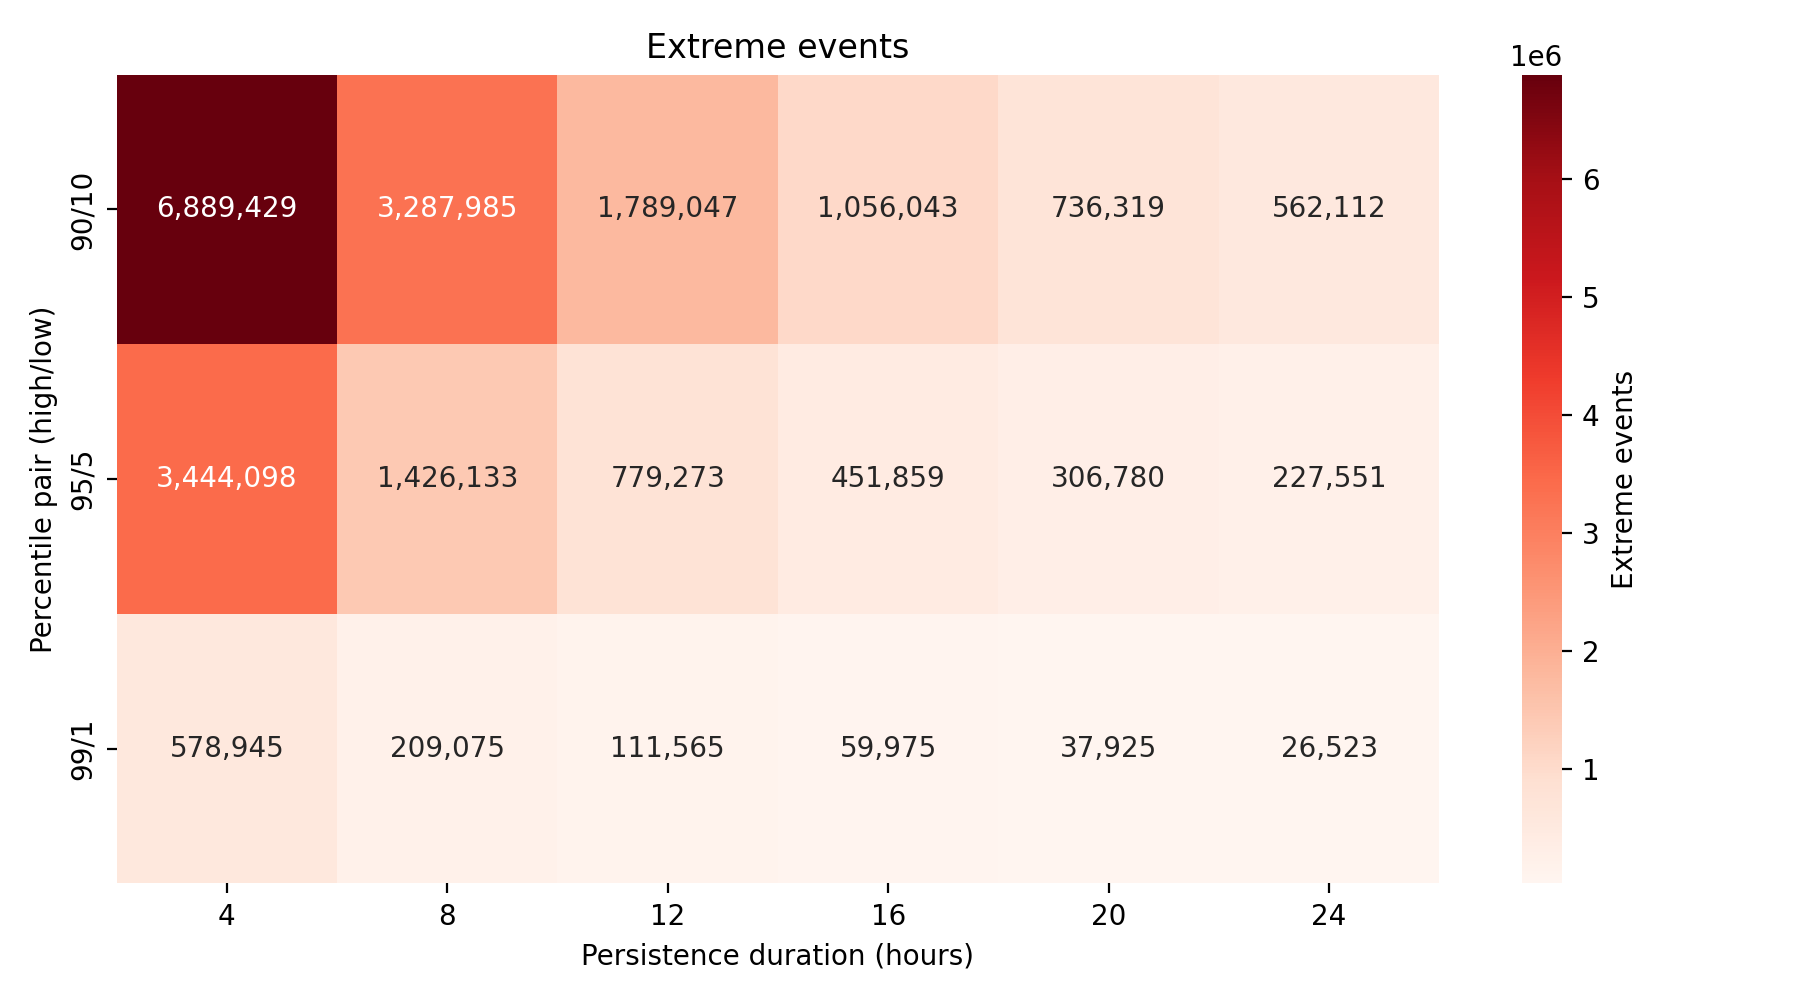
\includegraphics[width=0.8\textwidth]{figures/Q10_extreme_weather/era5_threshold_sensitivity_events_heatmap.png}
  \caption{Raw extreme-event counts (distinct persistence-qualifying spans, not hours) across the
  percentile-pair $\times$ persistence-duration sweep---the event-count companion to the hour
  counts in Figure~\ref{fig:extreme_hours_heatmap}.}
  \label{fig:app_extreme_events_heatmap}
\end{figure}

\begin{figure}[H]
  \centering
  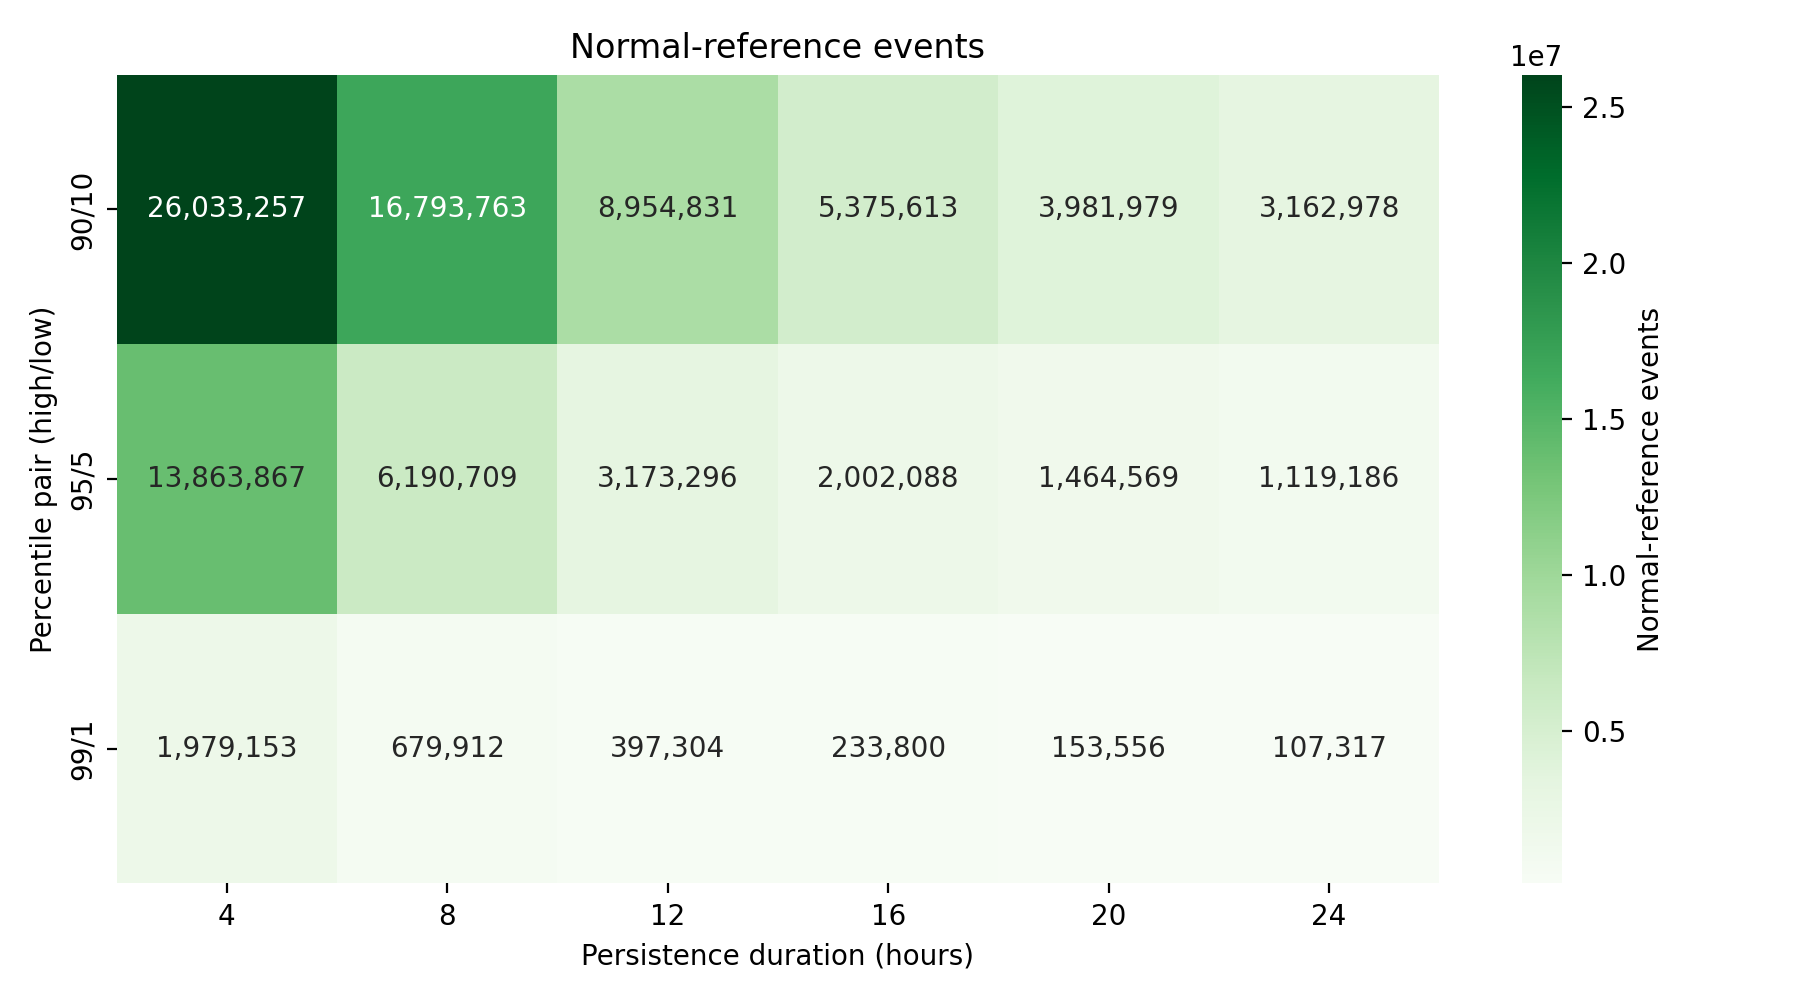
\includegraphics[width=0.8\textwidth]{figures/Q10_extreme_weather/era5_threshold_sensitivity_normal_events_heatmap.png}
  \caption{Raw normal-reference-event counts across the same sweep---the event-count companion to
  the hour counts in Figure~\ref{fig:normal_hours_heatmap}.}
  \label{fig:app_normal_events_heatmap}
\end{figure}
